\documentclass[final]{book}
\newcommand{\doctitle}{HSA Runtime Programmer's Reference Manual}
\newcommand{\docversion}{0.181}

\usepackage[T1]{fontenc}

\usepackage{ifdraft}
\usepackage[top=2.5cm,bottom=2.5cm,left=2.5cm,right=2.5cm]{geometry}

\usepackage[toc,page]{appendix}
\usepackage[usenames,dvipsnames,svgnames,table]{xcolor}
  \definecolor{lightgray}{gray}{0.9}
\usepackage{makeidx}
\usepackage[final]{graphicx}
\usepackage{sidecap}
\usepackage{float}

\usepackage[final]{listings}

\usepackage{longtable}

\usepackage{tikz}
\usetikzlibrary{arrows,automata,positioning,chains}
\tikzset{
        >=angle 45}

\usepackage{calc}
\catcode`\_=12

\usepackage{ifthen}
\usepackage{textcomp}

\usepackage{paralist}

\usepackage{framed}
\usepackage{times}
\usepackage[titles]{tocloft}
\usepackage{fancyhdr}

\usepackage{enumitem}

\usepackage{tcolorbox}
    \tcbuselibrary{breakable}

\usepackage{ifpdf}
\ifpdf
\usepackage[pdftex,
            bookmarks,
            final,             pagebackref=true,
            pdfpagemode=UseOutlines,             linktoc=all,              colorlinks=true,
            linkcolor=black,
            unicode
           ]{hyperref}
\else
\usepackage[ps2pdf,
            bookmarks,
            final,             pdfpagemode=UseOutlines,             linktoc=all,              pagebackref=true,
            colorlinks=true,
            linkcolor=black,
            unicode
           ]{hyperref}
\usepackage{pspicture}
\fi

\lstset{language=C++,
        inputencoding=utf8,
        basicstyle=\small,
        breaklines=true,
        breakatwhitespace=true,
        tabsize=4,
        showstringspaces=false,
        frame=none,
        backgroundcolor=\color{lightgray},
        keywordstyle=,
        emphstyle={\textbf},
        commentstyle=\color{ForestGreen},
        morecomment=[l][\color{green}]{\#}
}
\makeatletter{}\lstset{emph={hsa_status_string,hsa_init,hsa_shut_down,hsa_topology_object_ids,hsa_topology_object_descriptor,hsa_signal_create,hsa_signal_destroy,hsa_signal_load_acquire,hsa_signal_load_relaxed,hsa_signal_store_relaxed,hsa_signal_store_release,hsa_signal_exchange_release,hsa_signal_exchange_relaxed,hsa_signal_cas_release,hsa_signal_add_release,hsa_signal_add_relaxed,hsa_signal_subtract_release,hsa_signal_subtract_relaxed,hsa_signal_and_release,hsa_signal_and_relaxed,hsa_signal_or_release,hsa_signal_or_relaxed,hsa_signal_xor_release,hsa_signal_xor_relaxed,hsa_signal_wait_acquire,hsa_signal_wait_relaxed,hsa_signal_wait_timeout_acquire,hsa_signal_wait_timeout_relaxed,hsa_queue_create,hsa_queue_destroy,hsa_queue_inactivate,hsa_queue_load_read_index_relaxed,hsa_queue_load_read_index_acquire,hsa_queue_load_write_index_relaxed,hsa_queue_load_write_index_acquire,hsa_queue_store_write_index_relaxed,hsa_queue_store_write_index_release,hsa_queue_cas_write_index_relaxed,hsa_queue_cas_write_index_release,hsa_queue_cas_write_index_acquire,hsa_queue_cas_write_index_acquire_release,hsa_queue_add_write_index_relaxed,hsa_queue_add_write_index_acquire,hsa_queue_add_write_index_release,hsa_queue_add_write_index_acquire_release,hsa_queue_store_read_index_relaxed,hsa_queue_store_read_index_release,hsa_memory_register,hsa_memory_deregister,hsa_memory_allocate,hsa_memory_free,hsa_memory_allocate_kernarg,hsa_memory_free_kernarg,hsa_memory_copy_kernarg_to_system,hsa_memory_copy_system_to_kernarg,hsa_memory_allocate_component_local,hsa_memory_free_component_local,hsa_memory_copy_component_local_to_system,hsa_ext_finalize,hsa_ext_destroy_finalization_descriptor,hsa_ext_serialize_finalization_descriptor,hsa_ext_deserialize_finalization_descriptor,hsa_ext_program_create,hsa_ext_program_destroy,hsa_ext_add_module,hsa_ext_finalize_program,hsa_ext_query_program_agent_id,hsa_ext_query_program_agent_count,hsa_ext_query_program_agents,hsa_ext_query_program_module_count,hsa_ext_query_program_modules,hsa_ext_query_program_brig_module,hsa_ext_query_call_convention,hsa_ext_define_program_allocation_global_variable_address,hsa_ext_query_program_allocation_global_variable_address,hsa_ext_define_agent_allocation_global_variable_address,hsa_ext_query_agent_global_variable_address,hsa_ext_define_readonly_variable_address,hsa_ext_query_readonly_variable_address,hsa_ext_query_kernel_descriptor_address,hsa_ext_query_indirect_function_descriptor_address,hsa_ext_validate_program,hsa_ext_validate_program_module,hsa_ext_serialize_program,hsa_ext_deserialize_program,hsa_ext_image_get_format_capability,hsa_ext_image_get_info,hsa_ext_image_create_handle,hsa_ext_image_import,hsa_ext_image_export,hsa_ext_image_copy,hsa_ext_image_clear,hsa_ext_image_destroy_handle,hsa_ext_sampler_create_handle,hsa_ext_sampler_destroy_handle,hsa_register_agent_dispatch_callback,hsa_vendor_extension_query,hsa_extension_query,hsa_extension_query,}} 

\newcommand{\hsaarg}[1]{\textit{#1}}
\newcommand{\reffun}[1]{\textbf{#1}}
\newcommand{\refarg}[1]{\textit{#1}}
\newcommand{\reffld}[1]{\textit{#1}}
\newcommand{\reftyp}[1]{#1}
\newcommand{\refenu}[1]{\reftyp{#1}}
\newcommand{\refhsl}[1]{\reffun{#1}}

\usepackage{pdftexcmds}
\makeatletter{}\makeatletter
\newcommand{\hsaref}[1]{\ifnum\pdf@strcmp{#1}{blablablablabla}=0 blablablablabla
\else\ifnum\pdf@strcmp{#1}{hsa_status_t}=0\hyperlink{group__status_1gad755322e7ff95456520e8abdbe90d225}{\reftyp{hsa_\-status_\-t}}\else\ifnum\pdf@strcmp{#1}{HSA_STATUS_SUCCESS}=0\hyperlink{group__status_1ggad755322e7ff95456520e8abdbe90d225ae382ea0c9c05cce5a60d0317375159cc}{\refenu{HSA_\-STATUS_\-SUCCESS}}\else\ifnum\pdf@strcmp{#1}{HSA_EXT_STATUS_INFO_ALREADY_INITIALIZED}=0\hyperlink{group__status_1ggad755322e7ff95456520e8abdbe90d225a0882e3ebb9cc8a5c6033c43ee7a6d898}{\refenu{HSA_\-EXT_\-STATUS_\-INFO_\-ALREADY_\-INITIALIZED}}\else\ifnum\pdf@strcmp{#1}{HSA_EXT_STATUS_INFO_UNRECOGNIZED_OPTIONS}=0\hyperlink{group__status_1ggad755322e7ff95456520e8abdbe90d225a60343279bea68766b037297915b5f903}{\refenu{HSA_\-EXT_\-STATUS_\-INFO_\-UNRECOGNIZED_\-OPTIONS}}\else\ifnum\pdf@strcmp{#1}{HSA_STATUS_ERROR_WAIT_ABANDONED}=0\hyperlink{group__status_1ggad755322e7ff95456520e8abdbe90d225a3081a89b2b191a77f426b5697bca7360}{\refenu{HSA_\-STATUS_\-ERROR_\-WAIT_\-ABANDONED}}\else\ifnum\pdf@strcmp{#1}{HSA_STATUS_ERROR_INVALID_ARGUMENT}=0\hyperlink{group__status_1ggad755322e7ff95456520e8abdbe90d225ac7d3651f75107d2a6a8ba3b25683c030}{\refenu{HSA_\-STATUS_\-ERROR_\-INVALID_\-ARGUMENT}}\else\ifnum\pdf@strcmp{#1}{HSA_STATUS_ERROR_INVALID_COMPONENT}=0\hyperlink{group__status_1ggad755322e7ff95456520e8abdbe90d225ac136a6651d66e234971df5083600bbd0}{\refenu{HSA_\-STATUS_\-ERROR_\-INVALID_\-COMPONENT}}\else\ifnum\pdf@strcmp{#1}{HSA_STATUS_ERROR_INVALID_SIGNAL}=0\hyperlink{group__status_1ggad755322e7ff95456520e8abdbe90d225a7b4c8c0d4c99a1fe966abc2d39b575fe}{\refenu{HSA_\-STATUS_\-ERROR_\-INVALID_\-SIGNAL}}\else\ifnum\pdf@strcmp{#1}{HSA_STATUS_ERROR_INVALID_QUEUE}=0\hyperlink{group__status_1ggad755322e7ff95456520e8abdbe90d225aa3c762eb6a61b358702b45259d1686c4}{\refenu{HSA_\-STATUS_\-ERROR_\-INVALID_\-QUEUE}}\else\ifnum\pdf@strcmp{#1}{HSA_STATUS_ERROR_OUT_OF_RESOURCES}=0\hyperlink{group__status_1ggad755322e7ff95456520e8abdbe90d225a1a77fcf36d0d140874c4361ab093eff7}{\refenu{HSA_\-STATUS_\-ERROR_\-OUT_\-OF_\-RESOURCES}}\else\ifnum\pdf@strcmp{#1}{HSA_STATUS_ERROR_INVALID_PACKET_FORMAT}=0\hyperlink{group__status_1ggad755322e7ff95456520e8abdbe90d225a3fad45f72111eb99de5d8daef26c372c}{\refenu{HSA_\-STATUS_\-ERROR_\-INVALID_\-PACKET_\-FORMAT}}\else\ifnum\pdf@strcmp{#1}{HSA_STATUS_ERROR_SIGNAL_DEPENDENCY}=0\hyperlink{group__status_1ggad755322e7ff95456520e8abdbe90d225a160ebf19ea514abf81a8ac958c0e9f12}{\refenu{HSA_\-STATUS_\-ERROR_\-SIGNAL_\-DEPENDENCY}}\else\ifnum\pdf@strcmp{#1}{HSA_STATUS_ERROR_RESOURCE_FREE}=0\hyperlink{group__status_1ggad755322e7ff95456520e8abdbe90d225a6406af88203fcbec4179fbb71cc66b65}{\refenu{HSA_\-STATUS_\-ERROR_\-RESOURCE_\-FREE}}\else\ifnum\pdf@strcmp{#1}{HSA_STATUS_ERROR_NOT_REGISTERED}=0\hyperlink{group__status_1ggad755322e7ff95456520e8abdbe90d225a8b2f486dd206aa5545e8b0f2c1e2a568}{\refenu{HSA_\-STATUS_\-ERROR_\-NOT_\-REGISTERED}}\else\ifnum\pdf@strcmp{#1}{HSA_STATUS_ERROR_NOT_INITIALIZED}=0\hyperlink{group__status_1ggad755322e7ff95456520e8abdbe90d225a34ea59ade5bfce95eee935238a99f5b5}{\refenu{HSA_\-STATUS_\-ERROR_\-NOT_\-INITIALIZED}}\else\ifnum\pdf@strcmp{#1}{HSA_STATUS_ERROR_REFCOUNT_OVERFLOW}=0\hyperlink{group__status_1ggad755322e7ff95456520e8abdbe90d225aa9218eed04d1d2ffc5ed8f33f2cd1c9b}{\refenu{HSA_\-STATUS_\-ERROR_\-REFCOUNT_\-OVERFLOW}}\else\ifnum\pdf@strcmp{#1}{HSA_EXT_STATUS_ERROR_DIRECTIVE_MISMATCH}=0\hyperlink{group__status_1ggad755322e7ff95456520e8abdbe90d225ae16bcc443d027a0b880fd58f0443227b}{\refenu{HSA_\-EXT_\-STATUS_\-ERROR_\-DIRECTIVE_\-MISMATCH}}\else\ifnum\pdf@strcmp{#1}{HSA_EXT_STATUS_ERROR_IMAGE_FORMAT_UNSUPPORTED}=0\hyperlink{group__status_1ggad755322e7ff95456520e8abdbe90d225a42108181943a2d94749d95dc7942b7d0}{\refenu{HSA_\-EXT_\-STATUS_\-ERROR_\-IMAGE_\-FORMAT_\-UNSUPPORTED}}\else\ifnum\pdf@strcmp{#1}{HSA_EXT_STATUS_ERROR_IMAGE_SIZE_UNSUPPORTED}=0\hyperlink{group__status_1ggad755322e7ff95456520e8abdbe90d225a3ff898da367040b1f382c14c9f0a1bab}{\refenu{HSA_\-EXT_\-STATUS_\-ERROR_\-IMAGE_\-SIZE_\-UNSUPPORTED}}\else\ifnum\pdf@strcmp{#1}{hsa_status_string}=0\hyperlink{group__status_1ga72e5406b30241d3901ff0bd3907f4a7e}{\reffun{hsa_\-status_\-string}}\else\ifnum\pdf@strcmp{#1}{hsa_event_t}=0\hyperlink{group__status_1ga429d71a7f89eec75d076b4c6c3c131bf}{\reftyp{hsa_\-event_\-t}}\else\ifnum\pdf@strcmp{#1}{hsa_event_callback_t}=0\hyperlink{group__status_1ga8ac33c4e26296b067939e9cbbb25696a}{\reftyp{hsa_\-event_\-callback_\-t}}\else\ifnum\pdf@strcmp{#1}{hsa_powertwo8_t}=0\hyperlink{group__RuntimeCommon_1ga143c7c845aca213614c1d79b65c35a0c}{\reftyp{hsa_\-powertwo8_\-t}}\else\ifnum\pdf@strcmp{#1}{hsa_powertwo_t}=0\hyperlink{group__RuntimeCommon_1ga45e8c4edc00ad0dc2c9e6e14e8610977}{\reftyp{hsa_\-powertwo_\-t}}\else\ifnum\pdf@strcmp{#1}{HSA_POWERTWO_1}=0\hyperlink{group__RuntimeCommon_1gga45e8c4edc00ad0dc2c9e6e14e8610977a13bfa83a83c0f555efe4bbcca6b9cddf}{\refenu{HSA_\-POWERTWO_\-1}}\else\ifnum\pdf@strcmp{#1}{HSA_POWERTWO_2}=0\hyperlink{group__RuntimeCommon_1gga45e8c4edc00ad0dc2c9e6e14e8610977a465003dadda71ae8589097dd03202daf}{\refenu{HSA_\-POWERTWO_\-2}}\else\ifnum\pdf@strcmp{#1}{HSA_POWERTWO_4}=0\hyperlink{group__RuntimeCommon_1gga45e8c4edc00ad0dc2c9e6e14e8610977a04e128660c6aee9bd09b8be8683a4df9}{\refenu{HSA_\-POWERTWO_\-4}}\else\ifnum\pdf@strcmp{#1}{HSA_POWERTWO_8}=0\hyperlink{group__RuntimeCommon_1gga45e8c4edc00ad0dc2c9e6e14e8610977a6b602015c0db012f426e22c0354fbd05}{\refenu{HSA_\-POWERTWO_\-8}}\else\ifnum\pdf@strcmp{#1}{HSA_POWERTWO_16}=0\hyperlink{group__RuntimeCommon_1gga45e8c4edc00ad0dc2c9e6e14e8610977abc59007bbaea149704bb50a1aa70b7aa}{\refenu{HSA_\-POWERTWO_\-16}}\else\ifnum\pdf@strcmp{#1}{HSA_POWERTWO_32}=0\hyperlink{group__RuntimeCommon_1gga45e8c4edc00ad0dc2c9e6e14e8610977af13ebd4aecb93fd78bee555d26ed62a7}{\refenu{HSA_\-POWERTWO_\-32}}\else\ifnum\pdf@strcmp{#1}{HSA_POWERTWO_64}=0\hyperlink{group__RuntimeCommon_1gga45e8c4edc00ad0dc2c9e6e14e8610977a93252b7ad8bdcbec33390212e8897bd5}{\refenu{HSA_\-POWERTWO_\-64}}\else\ifnum\pdf@strcmp{#1}{HSA_POWERTWO_128}=0\hyperlink{group__RuntimeCommon_1gga45e8c4edc00ad0dc2c9e6e14e8610977ae78a1c50ad98ae134e34186acd52174e}{\refenu{HSA_\-POWERTWO_\-128}}\else\ifnum\pdf@strcmp{#1}{HSA_POWERTWO_256}=0\hyperlink{group__RuntimeCommon_1gga45e8c4edc00ad0dc2c9e6e14e8610977ae774bb9d85b5f7f9968ab76e50c23a6b}{\refenu{HSA_\-POWERTWO_\-256}}\else\ifnum\pdf@strcmp{#1}{hsa_dim3_t}=0\hyperlink{group__RuntimeCommon_1ga6f7883588491965c45382cd996351aa2}{\reftyp{hsa_\-dim3_\-t}}\else\ifnum\pdf@strcmp{#1}{hsa_dim_t}=0\hyperlink{group__RuntimeCommon_1gaa7eb83c51012a3b6f016f7b3388964ef}{\reftyp{hsa_\-dim_\-t}}\else\ifnum\pdf@strcmp{#1}{HSA_DIM_X}=0\hyperlink{group__RuntimeCommon_1ggaa7eb83c51012a3b6f016f7b3388964efa5a172a4cf084b71b9bafd68eaf159efc}{\refenu{HSA_\-DIM_\-X}}\else\ifnum\pdf@strcmp{#1}{HSA_DIM_Y}=0\hyperlink{group__RuntimeCommon_1ggaa7eb83c51012a3b6f016f7b3388964efa863557e1bf7f7ba4f7ac00527f214d0e}{\refenu{HSA_\-DIM_\-Y}}\else\ifnum\pdf@strcmp{#1}{HSA_DIM_Z}=0\hyperlink{group__RuntimeCommon_1ggaa7eb83c51012a3b6f016f7b3388964efaa2ea7a7aba09bb743508177f196d2983}{\refenu{HSA_\-DIM_\-Z}}\else\ifnum\pdf@strcmp{#1}{hsa_runtime_caller_t}=0\hyperlink{group__RuntimeCommon_1ga7d9b1191602415f5dd3893985cc93826}{\reftyp{hsa_\-runtime_\-caller_\-t}}\else\ifnum\pdf@strcmp{#1}{hsa_runtime_alloc_data_callback_t}=0\hyperlink{group__RuntimeCommon_1ga30804c05fe32b4ab9da480280dba8cc5}{\reftyp{hsa_\-runtime_\-alloc_\-data_\-callback_\-t}}\else\ifnum\pdf@strcmp{#1}{hsa_init}=0\hyperlink{group__initshutdown_1ga5b8574433e7dbcbd31ea397a02e3c32b}{\reffun{hsa_\-init}}\else\ifnum\pdf@strcmp{#1}{hsa_shut_down}=0\hyperlink{group__initshutdown_1ga97bdbccbd372609ad14a7ae7389cf4bf}{\reffun{hsa_\-shut_\-down}}\else\ifnum\pdf@strcmp{#1}{hsa_agent_type_t}=0\hyperlink{group__topology_1ga2e7880ed1215a49400af0a0039771876}{\reftyp{hsa_\-agent_\-type_\-t}}\else\ifnum\pdf@strcmp{#1}{HSA_AGENT_TYPE_HOST}=0\hyperlink{group__topology_1gga2e7880ed1215a49400af0a0039771876a6afb43ca46f3357a31a7720767cdb00c}{\refenu{HSA_\-AGENT_\-TYPE_\-HOST}}\else\ifnum\pdf@strcmp{#1}{HSA_AGENT_TYPE_COMPONENT}=0\hyperlink{group__topology_1gga2e7880ed1215a49400af0a0039771876aaf94199dff53355b7bf01912244f5b4b}{\refenu{HSA_\-AGENT_\-TYPE_\-COMPONENT}}\else\ifnum\pdf@strcmp{#1}{HSA_AGENT_TYPE_AGENT_DISPATCH}=0\hyperlink{group__topology_1gga2e7880ed1215a49400af0a0039771876af90ab87833b6a3db04b1eca68ea17825}{\refenu{HSA_\-AGENT_\-TYPE_\-AGENT_\-DISPATCH}}\else\ifnum\pdf@strcmp{#1}{hsa_agent_t}=0\hyperlink{group__topology_1gab8db3fb886332a24acac08ec361e1d86}{\reftyp{hsa_\-agent_\-t}}\else\ifnum\pdf@strcmp{#1}{hsa_segment_t}=0\hyperlink{group__topology_1ga8d13d587b03e1a9993af2c5089658f6d}{\reftyp{hsa_\-segment_\-t}}\else\ifnum\pdf@strcmp{#1}{hsa_memory_descriptor_t}=0\hyperlink{group__topology_1gafdcacbeb50c66179ae83ce8f0b447fbd}{\reftyp{hsa_\-memory_\-descriptor_\-t}}\else\ifnum\pdf@strcmp{#1}{hsa_cache_descriptor_t}=0\hyperlink{group__topology_1ga243c6e5a176770394cc09696a528210d}{\reftyp{hsa_\-cache_\-descriptor_\-t}}\else\ifnum\pdf@strcmp{#1}{hsa_topology_object_t}=0\hyperlink{group__topology_1ga6e6b13c8ff6a0a0eba273f31bb1ec11b}{\reftyp{hsa_\-topology_\-object_\-t}}\else\ifnum\pdf@strcmp{#1}{HSA_TOPOLOGY_OBJECT_AGENT}=0\hyperlink{group__topology_1gga6e6b13c8ff6a0a0eba273f31bb1ec11ba27b35495e288bd0d19c4d5dc3e758a7a}{\refenu{HSA_\-TOPOLOGY_\-OBJECT_\-AGENT}}\else\ifnum\pdf@strcmp{#1}{HSA_TOPOLOGY_OBJECT_MEMORY}=0\hyperlink{group__topology_1gga6e6b13c8ff6a0a0eba273f31bb1ec11ba7bc2442e7a668e766539f196f887bdbc}{\refenu{HSA_\-TOPOLOGY_\-OBJECT_\-MEMORY}}\else\ifnum\pdf@strcmp{#1}{HSA_TOPOLOGY_OBJECT_CACHE}=0\hyperlink{group__topology_1gga6e6b13c8ff6a0a0eba273f31bb1ec11ba6fa23678f9d1f6d71b7b9bafd6611247}{\refenu{HSA_\-TOPOLOGY_\-OBJECT_\-CACHE}}\else\ifnum\pdf@strcmp{#1}{hsa_topology_object_ids}=0\hyperlink{group__topology_1gade574cb89bfa01141b18c272b77d5743}{\reffun{hsa_\-topology_\-object_\-ids}}\else\ifnum\pdf@strcmp{#1}{hsa_topology_object_descriptor}=0\hyperlink{group__topology_1ga48ca22ea8268085106bb824ea80c7a17}{\reffun{hsa_\-topology_\-object_\-descriptor}}\else\ifnum\pdf@strcmp{#1}{hsa_signal_handle_t}=0\hyperlink{group__signals_1ga6592c136d70853d855bc11d9efdbf534}{\reftyp{hsa_\-signal_\-handle_\-t}}\else\ifnum\pdf@strcmp{#1}{hsa_signal_value_t}=0\hyperlink{group__signals_1gacdf7a070a2f988bcf97904a1f5d0e573}{\reftyp{hsa_\-signal_\-value_\-t}}\else\ifnum\pdf@strcmp{#1}{hsa_signal_create}=0\hyperlink{group__signals_1gac64f085f639ba66a8d28f008cc39724b}{\reffun{hsa_\-signal_\-create}}\else\ifnum\pdf@strcmp{#1}{hsa_signal_destroy}=0\hyperlink{group__signals_1ga3b76b9580215ab224967f6de976dc907}{\reffun{hsa_\-signal_\-destroy}}\else\ifnum\pdf@strcmp{#1}{hsa_signal_load_acquire}=0\hyperlink{group__signals_1ga12ce7ab1efe15c89db71680baeb7732e}{\reffun{hsa_\-signal_\-load_\-acquire}}\else\ifnum\pdf@strcmp{#1}{hsa_signal_load_relaxed}=0\hyperlink{group__signals_1ga7a6ee38287493f10b4e285d0f7555a69}{\reffun{hsa_\-signal_\-load_\-relaxed}}\else\ifnum\pdf@strcmp{#1}{hsa_signal_store_relaxed}=0\hyperlink{group__signals_1ga459356a08e9f67338d5ca71ab55ee930}{\reffun{hsa_\-signal_\-store_\-relaxed}}\else\ifnum\pdf@strcmp{#1}{hsa_signal_store_release}=0\hyperlink{group__signals_1gaa2d456b111870ba56fa5461a5d246289}{\reffun{hsa_\-signal_\-store_\-release}}\else\ifnum\pdf@strcmp{#1}{hsa_signal_exchange_release}=0\hyperlink{group__signals_1gae6179424d96bd22a5eafca70b5724d6b}{\reffun{hsa_\-signal_\-exchange_\-release}}\else\ifnum\pdf@strcmp{#1}{hsa_signal_exchange_relaxed}=0\hyperlink{group__signals_1gae67f1205f49e846c1c919b0ed885b9c1}{\reffun{hsa_\-signal_\-exchange_\-relaxed}}\else\ifnum\pdf@strcmp{#1}{hsa_signal_cas_release}=0\hyperlink{group__signals_1ga3fe687b7431dc93a1b5049a9abfa9e5b}{\reffun{hsa_\-signal_\-cas_\-release}}\else\ifnum\pdf@strcmp{#1}{hsa_signal_add_release}=0\hyperlink{group__signals_1ga3edf8c18628f4d35e6bb679eacc196c7}{\reffun{hsa_\-signal_\-add_\-release}}\else\ifnum\pdf@strcmp{#1}{hsa_signal_add_relaxed}=0\hyperlink{group__signals_1ga65ed15c44507c0039349898a92ec9623}{\reffun{hsa_\-signal_\-add_\-relaxed}}\else\ifnum\pdf@strcmp{#1}{hsa_signal_subtract_release}=0\hyperlink{group__signals_1gab3a11cc434dc4b314b30d74d49bdc352}{\reffun{hsa_\-signal_\-subtract_\-release}}\else\ifnum\pdf@strcmp{#1}{hsa_signal_subtract_relaxed}=0\hyperlink{group__signals_1ga07462947d39b47257c24cb1cda32ed99}{\reffun{hsa_\-signal_\-subtract_\-relaxed}}\else\ifnum\pdf@strcmp{#1}{hsa_signal_and_release}=0\hyperlink{group__signals_1gaa7889346cc882e8faba6570b5e8d1c79}{\reffun{hsa_\-signal_\-and_\-release}}\else\ifnum\pdf@strcmp{#1}{hsa_signal_and_relaxed}=0\hyperlink{group__signals_1gaa21029528b38855f041a42a2779e021e}{\reffun{hsa_\-signal_\-and_\-relaxed}}\else\ifnum\pdf@strcmp{#1}{hsa_signal_or_release}=0\hyperlink{group__signals_1ga4c988e5d4663e1c111074dfbeb5cbafa}{\reffun{hsa_\-signal_\-or_\-release}}\else\ifnum\pdf@strcmp{#1}{hsa_signal_or_relaxed}=0\hyperlink{group__signals_1gabb0df851fe1a61a413bc3cd8e81f493a}{\reffun{hsa_\-signal_\-or_\-relaxed}}\else\ifnum\pdf@strcmp{#1}{hsa_signal_xor_release}=0\hyperlink{group__signals_1ga18ad4d4c7ca388263d367b635e14372a}{\reffun{hsa_\-signal_\-xor_\-release}}\else\ifnum\pdf@strcmp{#1}{hsa_signal_xor_relaxed}=0\hyperlink{group__signals_1ga662b68a16438f18d689f9b9f534b0b68}{\reffun{hsa_\-signal_\-xor_\-relaxed}}\else\ifnum\pdf@strcmp{#1}{hsa_signal_condition_t}=0\hyperlink{group__signals_1gab7190fcff48c6dbeded341389ed17c8d}{\reftyp{hsa_\-signal_\-condition_\-t}}\else\ifnum\pdf@strcmp{#1}{HSA_EQ}=0\hyperlink{group__signals_1ggab7190fcff48c6dbeded341389ed17c8daad3556497ba9c0d287d42345baba25d6}{\refenu{HSA_\-EQ}}\else\ifnum\pdf@strcmp{#1}{HSA_NE}=0\hyperlink{group__signals_1ggab7190fcff48c6dbeded341389ed17c8dae595f91b4c0720a4741c6fe4ead6f793}{\refenu{HSA_\-NE}}\else\ifnum\pdf@strcmp{#1}{HSA_LT}=0\hyperlink{group__signals_1ggab7190fcff48c6dbeded341389ed17c8da02c24632d8b8925649d95f4221b40e15}{\refenu{HSA_\-LT}}\else\ifnum\pdf@strcmp{#1}{HSA_GTE}=0\hyperlink{group__signals_1ggab7190fcff48c6dbeded341389ed17c8da8f171d683f208e4e9794b89f40998547}{\refenu{HSA_\-GTE}}\else\ifnum\pdf@strcmp{#1}{hsa_signal_wait_acquire}=0\hyperlink{group__signals_1ga882725c4930673915c174bb5dd56cb23}{\reffun{hsa_\-signal_\-wait_\-acquire}}\else\ifnum\pdf@strcmp{#1}{hsa_signal_wait_relaxed}=0\hyperlink{group__signals_1ga328b24eb4b4633a1370834820d5bf9d2}{\reffun{hsa_\-signal_\-wait_\-relaxed}}\else\ifnum\pdf@strcmp{#1}{hsa_signal_wait_timeout_acquire}=0\hyperlink{group__signals_1gabe68135cd6a2b116d91e5ac4ed53db9a}{\reffun{hsa_\-signal_\-wait_\-timeout_\-acquire}}\else\ifnum\pdf@strcmp{#1}{hsa_signal_wait_timeout_relaxed}=0\hyperlink{group__signals_1gaed306c1c7a65c2681cc9a42825a548ad}{\reffun{hsa_\-signal_\-wait_\-timeout_\-relaxed}}\else\ifnum\pdf@strcmp{#1}{hsa_queue_type_t}=0\hyperlink{group__queue_1gaf1939f228a41fa6ee50cffd4de03b561}{\reftyp{hsa_\-queue_\-type_\-t}}\else\ifnum\pdf@strcmp{#1}{HSA_QUEUE_TYPE_MULTI}=0\hyperlink{group__queue_1ggaf1939f228a41fa6ee50cffd4de03b561abb25665f0708270e16e6c400c097c88b}{\refenu{HSA_\-QUEUE_\-TYPE_\-MULTI}}\else\ifnum\pdf@strcmp{#1}{HSA_QUEUE_TYPE_SINGLE}=0\hyperlink{group__queue_1ggaf1939f228a41fa6ee50cffd4de03b561a45c3277e4e4fcb8a9788081549551f0a}{\refenu{HSA_\-QUEUE_\-TYPE_\-SINGLE}}\else\ifnum\pdf@strcmp{#1}{hsa_queue_feature_t}=0\hyperlink{group__queue_1ga1145b01f6d9e2670179a22c92db39413}{\reftyp{hsa_\-queue_\-feature_\-t}}\else\ifnum\pdf@strcmp{#1}{HSA_QUEUE_FEATURE_DISPATCH}=0\hyperlink{group__queue_1gga1145b01f6d9e2670179a22c92db39413a838cfd25a87de1dd5c0205beea2642e3}{\refenu{HSA_\-QUEUE_\-FEATURE_\-DISPATCH}}\else\ifnum\pdf@strcmp{#1}{HSA_QUEUE_FEATURE_AGENT_DISPATCH}=0\hyperlink{group__queue_1gga1145b01f6d9e2670179a22c92db39413a3c16b42876eacbb11d9b2e7a5488dede}{\refenu{HSA_\-QUEUE_\-FEATURE_\-AGENT_\-DISPATCH}}\else\ifnum\pdf@strcmp{#1}{hsa_queue_t}=0\hyperlink{group__queue_1gacbb2835331f18aee30ee441f07b3fc5a}{\reftyp{hsa_\-queue_\-t}}\else\ifnum\pdf@strcmp{#1}{hsa_queue_create}=0\hyperlink{group__queue_1gad922ac264b223f1ba8779b0705dea163}{\reffun{hsa_\-queue_\-create}}\else\ifnum\pdf@strcmp{#1}{hsa_queue_destroy}=0\hyperlink{group__queue_1ga2669dc4c7190f2ba65b453110a92ceb5}{\reffun{hsa_\-queue_\-destroy}}\else\ifnum\pdf@strcmp{#1}{hsa_queue_inactivate}=0\hyperlink{group__queue_1gac3fe6420d5b57a27cc453f97ccff3125}{\reffun{hsa_\-queue_\-inactivate}}\else\ifnum\pdf@strcmp{#1}{hsa_queue_load_read_index_relaxed}=0\hyperlink{group__queue_1gafcfb453ee6f35c7d768cba3163804bed}{\reffun{hsa_\-queue_\-load_\-read_\-index_\-relaxed}}\else\ifnum\pdf@strcmp{#1}{hsa_queue_load_read_index_acquire}=0\hyperlink{group__queue_1gab2468ee27d925edf3d30f4c3c3143642}{\reffun{hsa_\-queue_\-load_\-read_\-index_\-acquire}}\else\ifnum\pdf@strcmp{#1}{hsa_queue_load_write_index_relaxed}=0\hyperlink{group__queue_1ga2f31d20692bb769f3b1dfaea115ffd92}{\reffun{hsa_\-queue_\-load_\-write_\-index_\-relaxed}}\else\ifnum\pdf@strcmp{#1}{hsa_queue_load_write_index_acquire}=0\hyperlink{group__queue_1gab84efedb23078a1222bad3f20199565a}{\reffun{hsa_\-queue_\-load_\-write_\-index_\-acquire}}\else\ifnum\pdf@strcmp{#1}{hsa_queue_store_write_index_relaxed}=0\hyperlink{group__queue_1gae97a3c68e2adae8da25840d13b8bc8e0}{\reffun{hsa_\-queue_\-store_\-write_\-index_\-relaxed}}\else\ifnum\pdf@strcmp{#1}{hsa_queue_store_write_index_release}=0\hyperlink{group__queue_1ga105a5569dfc76284a633af4c983c23ea}{\reffun{hsa_\-queue_\-store_\-write_\-index_\-release}}\else\ifnum\pdf@strcmp{#1}{hsa_queue_cas_write_index_relaxed}=0\hyperlink{group__queue_1gac64736b757622a7151102afe34a40599}{\reffun{hsa_\-queue_\-cas_\-write_\-index_\-relaxed}}\else\ifnum\pdf@strcmp{#1}{hsa_queue_cas_write_index_release}=0\hyperlink{group__queue_1ga6a2f344e1337c5aed26363fb10a39254}{\reffun{hsa_\-queue_\-cas_\-write_\-index_\-release}}\else\ifnum\pdf@strcmp{#1}{hsa_queue_cas_write_index_acquire}=0\hyperlink{group__queue_1gad497720ffc7d3168a1deb2f89fb900c8}{\reffun{hsa_\-queue_\-cas_\-write_\-index_\-acquire}}\else\ifnum\pdf@strcmp{#1}{hsa_queue_cas_write_index_acquire_release}=0\hyperlink{group__queue_1gaad03aee6f7f3a0bf65e479540147279b}{\reffun{hsa_\-queue_\-cas_\-write_\-index_\-acquire_\-release}}\else\ifnum\pdf@strcmp{#1}{hsa_queue_add_write_index_relaxed}=0\hyperlink{group__queue_1ga29a1dd653298cc08c756da30bd58015b}{\reffun{hsa_\-queue_\-add_\-write_\-index_\-relaxed}}\else\ifnum\pdf@strcmp{#1}{hsa_queue_add_write_index_acquire}=0\hyperlink{group__queue_1ga2acde719c68cf402bfcef4b429775039}{\reffun{hsa_\-queue_\-add_\-write_\-index_\-acquire}}\else\ifnum\pdf@strcmp{#1}{hsa_queue_add_write_index_release}=0\hyperlink{group__queue_1ga84aa64c593280183028a0d140b960726}{\reffun{hsa_\-queue_\-add_\-write_\-index_\-release}}\else\ifnum\pdf@strcmp{#1}{hsa_queue_add_write_index_acquire_release}=0\hyperlink{group__queue_1ga576e17ddd84ace09fb9c02516ddb6eef}{\reffun{hsa_\-queue_\-add_\-write_\-index_\-acquire_\-release}}\else\ifnum\pdf@strcmp{#1}{hsa_queue_store_read_index_relaxed}=0\hyperlink{group__queue_1ga3862242b38d3711355844027582a82c5}{\reffun{hsa_\-queue_\-store_\-read_\-index_\-relaxed}}\else\ifnum\pdf@strcmp{#1}{hsa_queue_store_read_index_release}=0\hyperlink{group__queue_1ga46c9fbf6dc7dbb1a136a7787921624c4}{\reffun{hsa_\-queue_\-store_\-read_\-index_\-release}}\else\ifnum\pdf@strcmp{#1}{hsa_aql_packet_format_t}=0\hyperlink{group__aql_1ga21e03ac6edb26e457468af5fe501b7ad}{\reftyp{hsa_\-aql_\-packet_\-format_\-t}}\else\ifnum\pdf@strcmp{#1}{HSA_AQL_PACKET_FORMAT_ALWAYS_RESERVED}=0\hyperlink{group__aql_1gga21e03ac6edb26e457468af5fe501b7adaaa022c87937de2531388a681182e4d36}{\refenu{HSA_\-AQL_\-PACKET_\-FORMAT_\-ALWAYS_\-RESERVED}}\else\ifnum\pdf@strcmp{#1}{HSA_AQL_PACKET_FORMAT_INVALID}=0\hyperlink{group__aql_1gga21e03ac6edb26e457468af5fe501b7adadc0bb64d5b0037718e716d57f6befb6a}{\refenu{HSA_\-AQL_\-PACKET_\-FORMAT_\-INVALID}}\else\ifnum\pdf@strcmp{#1}{HSA_AQL_PACKET_FORMAT_DISPATCH}=0\hyperlink{group__aql_1gga21e03ac6edb26e457468af5fe501b7ada90d2a5dbd40f372f777402c83edf9d86}{\refenu{HSA_\-AQL_\-PACKET_\-FORMAT_\-DISPATCH}}\else\ifnum\pdf@strcmp{#1}{HSA_AQL_PACKET_FORMAT_BARRIER}=0\hyperlink{group__aql_1gga21e03ac6edb26e457468af5fe501b7adadaf10ccf48d374dfa87b7ad237a1788d}{\refenu{HSA_\-AQL_\-PACKET_\-FORMAT_\-BARRIER}}\else\ifnum\pdf@strcmp{#1}{HSA_AQL_PACKET_FORMAT_AGENT_DISPATCH}=0\hyperlink{group__aql_1gga21e03ac6edb26e457468af5fe501b7ada5189936e5f67be9e3463465aed69b008}{\refenu{HSA_\-AQL_\-PACKET_\-FORMAT_\-AGENT_\-DISPATCH}}\else\ifnum\pdf@strcmp{#1}{hsa_fence_scope_t}=0\hyperlink{group__aql_1ga6c1a86878de5b0f980202ad7e4e8d42a}{\reftyp{hsa_\-fence_\-scope_\-t}}\else\ifnum\pdf@strcmp{#1}{HSA_FENCE_SCOPE_NONE}=0\hyperlink{group__aql_1gga6c1a86878de5b0f980202ad7e4e8d42aa5dc7b942cd56f91094a088435027be2c}{\refenu{HSA_\-FENCE_\-SCOPE_\-NONE}}\else\ifnum\pdf@strcmp{#1}{HSA_FENCE_SCOPE_COMPONENT}=0\hyperlink{group__aql_1gga6c1a86878de5b0f980202ad7e4e8d42aa9818589db02bc7c0639652eccd64c95d}{\refenu{HSA_\-FENCE_\-SCOPE_\-COMPONENT}}\else\ifnum\pdf@strcmp{#1}{HSA_FENCE_SCOPE_SYSTEM}=0\hyperlink{group__aql_1gga6c1a86878de5b0f980202ad7e4e8d42aa6ecb203c10f12ec4bcf475d527c3a870}{\refenu{HSA_\-FENCE_\-SCOPE_\-SYSTEM}}\else\ifnum\pdf@strcmp{#1}{hsa_aql_packet_header_t}=0\hyperlink{group__aql_1ga92558e047d003985bae2558febd3dd40}{\reftyp{hsa_\-aql_\-packet_\-header_\-t}}\else\ifnum\pdf@strcmp{#1}{hsa_aql_dispatch_packet_t}=0\hyperlink{group__aql_1gab3d5ded5ac53f70931768468c0c0cfd6}{\reftyp{hsa_\-aql_\-dispatch_\-packet_\-t}}\else\ifnum\pdf@strcmp{#1}{hsa_aql_agent_dispatch_packet_t}=0\hyperlink{group__aql_1ga07dc7a6c787b5bee6e3f0b8b79586109}{\reftyp{hsa_\-aql_\-agent_\-dispatch_\-packet_\-t}}\else\ifnum\pdf@strcmp{#1}{hsa_aql_barrier_packet_t}=0\hyperlink{group__aql_1ga8e5ebbeffbf5af1ece8db9ef27c14715}{\reftyp{hsa_\-aql_\-barrier_\-packet_\-t}}\else\ifnum\pdf@strcmp{#1}{hsa_memory_register}=0\hyperlink{group__memory_1gaa4d4efc5ba903ea29587392aa1c8a267}{\reffun{hsa_\-memory_\-register}}\else\ifnum\pdf@strcmp{#1}{hsa_memory_deregister}=0\hyperlink{group__memory_1ga05508ed130cdd83aeab76db3328a45fc}{\reffun{hsa_\-memory_\-deregister}}\else\ifnum\pdf@strcmp{#1}{hsa_memory_allocate}=0\hyperlink{group__memory_1ga54b95840aafe4301a6c8cccea624f6e8}{\reffun{hsa_\-memory_\-allocate}}\else\ifnum\pdf@strcmp{#1}{hsa_memory_free}=0\hyperlink{group__memory_1gaf968e8053981351ec0b16a04aeb51a8e}{\reffun{hsa_\-memory_\-free}}\else\ifnum\pdf@strcmp{#1}{hsa_memory_allocate_kernarg}=0\hyperlink{group__memory_1gaa26de25e2d7c7b8d96f5c2606d0b39a2}{\reffun{hsa_\-memory_\-allocate_\-kernarg}}\else\ifnum\pdf@strcmp{#1}{hsa_memory_free_kernarg}=0\hyperlink{group__memory_1gad585b1a966ffee1e0df23647de40237a}{\reffun{hsa_\-memory_\-free_\-kernarg}}\else\ifnum\pdf@strcmp{#1}{hsa_memory_copy_kernarg_to_system}=0\hyperlink{group__memory_1ga85b2081cde17a1bedd4027c196681be5}{\reffun{hsa_\-memory_\-copy_\-kernarg_\-to_\-system}}\else\ifnum\pdf@strcmp{#1}{hsa_memory_copy_system_to_kernarg}=0\hyperlink{group__memory_1ga34251efd3fcba21ab16c5c42eb27032f}{\reffun{hsa_\-memory_\-copy_\-system_\-to_\-kernarg}}\else\ifnum\pdf@strcmp{#1}{hsa_memory_allocate_component_local}=0\hyperlink{group__memory_1ga36a7f7550f61cfff55c566ee0ebc1be5}{\reffun{hsa_\-memory_\-allocate_\-component_\-local}}\else\ifnum\pdf@strcmp{#1}{hsa_memory_free_component_local}=0\hyperlink{group__memory_1ga8f5353d063822f29295bddc230637817}{\reffun{hsa_\-memory_\-free_\-component_\-local}}\else\ifnum\pdf@strcmp{#1}{hsa_memory_copy_component_local_to_system}=0\hyperlink{group__memory_1ga292a4a5210b402fbf4320197d1cd3264}{\reffun{hsa_\-memory_\-copy_\-component_\-local_\-to_\-system}}\else\ifnum\pdf@strcmp{#1}{hsa_ext_brig_profile8_t}=0\hyperlink{group__FinalizerCoreApi_1ga4d058e43da41c147915dbe70cace9947}{\reftyp{hsa_\-ext_\-brig_\-profile8_\-t}}\else\ifnum\pdf@strcmp{#1}{hsa_ext_brig_profile_t}=0\hyperlink{group__FinalizerCoreApi_1gaf65d6aea5a7200a4300f65306c08ea6e}{\reftyp{hsa_\-ext_\-brig_\-profile_\-t}}\else\ifnum\pdf@strcmp{#1}{HSA_EXT_BRIG_PROFILE_BASE}=0\hyperlink{group__FinalizerCoreApi_1ggaf65d6aea5a7200a4300f65306c08ea6eadf0f501825c2f687f94fba6c2288d563}{\refenu{HSA_\-EXT_\-BRIG_\-PROFILE_\-BASE}}\else\ifnum\pdf@strcmp{#1}{HSA_EXT_BRIG_PROFILE_FULL}=0\hyperlink{group__FinalizerCoreApi_1ggaf65d6aea5a7200a4300f65306c08ea6ea89285e7d3e3f19217df4e8f987c4126c}{\refenu{HSA_\-EXT_\-BRIG_\-PROFILE_\-FULL}}\else\ifnum\pdf@strcmp{#1}{hsa_ext_brig_machine_model8_t}=0\hyperlink{group__FinalizerCoreApi_1ga5030b76e1c72556f42a7dc7eebab16df}{\reftyp{hsa_\-ext_\-brig_\-machine_\-model8_\-t}}\else\ifnum\pdf@strcmp{#1}{hsa_ext_brig_machine_model_t}=0\hyperlink{group__FinalizerCoreApi_1ga2079a73d7b54be5bb13026bac890dcbc}{\reftyp{hsa_\-ext_\-brig_\-machine_\-model_\-t}}\else\ifnum\pdf@strcmp{#1}{HSA_EXT_BRIG_MACHINE_SMALL}=0\hyperlink{group__FinalizerCoreApi_1gga2079a73d7b54be5bb13026bac890dcbca4d88cee5853fe4b072890619202c5b56}{\refenu{HSA_\-EXT_\-BRIG_\-MACHINE_\-SMALL}}\else\ifnum\pdf@strcmp{#1}{HSA_EXT_BRIG_MACHINE_LARGE}=0\hyperlink{group__FinalizerCoreApi_1gga2079a73d7b54be5bb13026bac890dcbca1d8a69a16cc565b2427ca590400081ef}{\refenu{HSA_\-EXT_\-BRIG_\-MACHINE_\-LARGE}}\else\ifnum\pdf@strcmp{#1}{hsa_ext_brig_section_id32_t}=0\hyperlink{group__FinalizerCoreApi_1ga2b753bccbe39c51384d6fa31a2302f0c}{\reftyp{hsa_\-ext_\-brig_\-section_\-id32_\-t}}\else\ifnum\pdf@strcmp{#1}{hsa_ext_brig_section_id_t}=0\hyperlink{group__FinalizerCoreApi_1ga3060576486841364f0842a76810aea06}{\reftyp{hsa_\-ext_\-brig_\-section_\-id_\-t}}\else\ifnum\pdf@strcmp{#1}{HSA_EXT_BRIG_SECTION_DATA}=0\hyperlink{group__FinalizerCoreApi_1gga3060576486841364f0842a76810aea06a9b040e9aae3efa23134666d054a3a839}{\refenu{HSA_\-EXT_\-BRIG_\-SECTION_\-DATA}}\else\ifnum\pdf@strcmp{#1}{HSA_EXT_BRIG_SECTION_CODE}=0\hyperlink{group__FinalizerCoreApi_1gga3060576486841364f0842a76810aea06a43997c8d8ab6c03c301c949bdb1819c7}{\refenu{HSA_\-EXT_\-BRIG_\-SECTION_\-CODE}}\else\ifnum\pdf@strcmp{#1}{HSA_EXT_BRIG_SECTION_OPERAND}=0\hyperlink{group__FinalizerCoreApi_1gga3060576486841364f0842a76810aea06ae52428f823f64d4ad9a0d8e2e29aea0b}{\refenu{HSA_\-EXT_\-BRIG_\-SECTION_\-OPERAND}}\else\ifnum\pdf@strcmp{#1}{hsa_ext_brig_section_header_t}=0\hyperlink{group__FinalizerCoreApi_1gaf9d6f363926d83463e8458aa5b5b0cf6}{\reftyp{hsa_\-ext_\-brig_\-section_\-header_\-t}}\else\ifnum\pdf@strcmp{#1}{hsa_ext_brig_module_t}=0\hyperlink{group__FinalizerCoreApi_1ga104477d24306200a2847b44c325e312a}{\reftyp{hsa_\-ext_\-brig_\-module_\-t}}\else\ifnum\pdf@strcmp{#1}{hsa_ext_brig_module_handle_t}=0\hyperlink{group__FinalizerCoreApi_1ga0216996f5341a8591ecf9e0f6fd1b7e5}{\reftyp{hsa_\-ext_\-brig_\-module_\-handle_\-t}}\else\ifnum\pdf@strcmp{#1}{hsa_ext_brig_code_section_offset32_t}=0\hyperlink{group__FinalizerCoreApi_1ga494b8ac14a8c10af95b83b51a8a4ad7f}{\reftyp{hsa_\-ext_\-brig_\-code_\-section_\-offset32_\-t}}\else\ifnum\pdf@strcmp{#1}{hsa_ext_exception_kind16_t}=0\hyperlink{group__FinalizerCoreApi_1gaf05e7b6c47e7baac1cc9fb203047f168}{\reftyp{hsa_\-ext_\-exception_\-kind16_\-t}}\else\ifnum\pdf@strcmp{#1}{hsa_ext_exception_kind_t}=0\hyperlink{group__FinalizerCoreApi_1gaac4b20de831dd17c83c1e2110bac0ef2}{\reftyp{hsa_\-ext_\-exception_\-kind_\-t}}\else\ifnum\pdf@strcmp{#1}{HSA_EXT_EXCEPTION_INVALID_OPERATION}=0\hyperlink{group__FinalizerCoreApi_1ggaac4b20de831dd17c83c1e2110bac0ef2af3acf5b85fdfd50083ba20eb4142bb9f}{\refenu{HSA_\-EXT_\-EXCEPTION_\-INVALID_\-OPERATION}}\else\ifnum\pdf@strcmp{#1}{HSA_EXT_EXCEPTION_DIVIDE_BY_ZERO}=0\hyperlink{group__FinalizerCoreApi_1ggaac4b20de831dd17c83c1e2110bac0ef2adf54889632462cdeb6bbf4f36d0f630c}{\refenu{HSA_\-EXT_\-EXCEPTION_\-DIVIDE_\-BY_\-ZERO}}\else\ifnum\pdf@strcmp{#1}{HSA_EXT_EXCEPTION_OVERFLOW}=0\hyperlink{group__FinalizerCoreApi_1ggaac4b20de831dd17c83c1e2110bac0ef2a3cffa261ec9fbb0910b0ed11ea17126e}{\refenu{HSA_\-EXT_\-EXCEPTION_\-OVERFLOW}}\else\ifnum\pdf@strcmp{#1}{HSA_EXT_EXCEPTION_UNDERFLOW}=0\hyperlink{group__FinalizerCoreApi_1ggaac4b20de831dd17c83c1e2110bac0ef2a15e11888d04953c37f86c8870807c888}{\refenu{HSA_\-EXT_\-EXCEPTION_\-UNDERFLOW}}\else\ifnum\pdf@strcmp{#1}{HSA_EXT_EXCEPTION_INEXACT}=0\hyperlink{group__FinalizerCoreApi_1ggaac4b20de831dd17c83c1e2110bac0ef2ab0a718c671deb5e84e350199db22a24b}{\refenu{HSA_\-EXT_\-EXCEPTION_\-INEXACT}}\else\ifnum\pdf@strcmp{#1}{hsa_ext_control_directive_present64_t}=0\hyperlink{group__FinalizerCoreApi_1ga366dea916dc7cec2954369e132e395e3}{\reftyp{hsa_\-ext_\-control_\-directive_\-present64_\-t}}\else\ifnum\pdf@strcmp{#1}{hsa_ext_control_directive_present_t}=0\hyperlink{group__FinalizerCoreApi_1ga143d9e622dfd7889d52fb5eb5ed1ffdb}{\reftyp{hsa_\-ext_\-control_\-directive_\-present_\-t}}\else\ifnum\pdf@strcmp{#1}{HSA_EXT_CONTROL_DIRECTIVE_ENABLE_BREAK_EXCEPTIONS}=0\hyperlink{group__FinalizerCoreApi_1gga143d9e622dfd7889d52fb5eb5ed1ffdba1c209f3a9fd22b358006c221303f8893}{\refenu{HSA_\-EXT_\-CONTROL_\-DIRECTIVE_\-ENABLE_\-BREAK_\-EXCEPTIONS}}\else\ifnum\pdf@strcmp{#1}{HSA_EXT_CONTROL_DIRECTIVE_ENABLE_DETECT_EXCEPTIONS}=0\hyperlink{group__FinalizerCoreApi_1gga143d9e622dfd7889d52fb5eb5ed1ffdba5f6e061c9abd08976ee6f4c4ee48f30a}{\refenu{HSA_\-EXT_\-CONTROL_\-DIRECTIVE_\-ENABLE_\-DETECT_\-EXCEPTIONS}}\else\ifnum\pdf@strcmp{#1}{HSA_EXT_CONTROL_DIRECTIVE_MAX_DYNAMIC_GROUP_SIZE}=0\hyperlink{group__FinalizerCoreApi_1gga143d9e622dfd7889d52fb5eb5ed1ffdba7787b99c887699ca6fe8d1cd4de3477e}{\refenu{HSA_\-EXT_\-CONTROL_\-DIRECTIVE_\-MAX_\-DYNAMIC_\-GROUP_\-SIZE}}\else\ifnum\pdf@strcmp{#1}{HSA_EXT_CONTROL_DIRECTIVE_MAX_FLAT_GRID_SIZE}=0\hyperlink{group__FinalizerCoreApi_1gga143d9e622dfd7889d52fb5eb5ed1ffdba8f84c9f5303be293df76bf82b002299c}{\refenu{HSA_\-EXT_\-CONTROL_\-DIRECTIVE_\-MAX_\-FLAT_\-GRID_\-SIZE}}\else\ifnum\pdf@strcmp{#1}{HSA_EXT_CONTROL_DIRECTIVE_MAX_FLAT_WORKGROUP_SIZE}=0\hyperlink{group__FinalizerCoreApi_1gga143d9e622dfd7889d52fb5eb5ed1ffdbaa0e6d7d860284c6cadde5c7e9db66968}{\refenu{HSA_\-EXT_\-CONTROL_\-DIRECTIVE_\-MAX_\-FLAT_\-WORKGROUP_\-SIZE}}\else\ifnum\pdf@strcmp{#1}{HSA_EXT_CONTROL_DIRECTIVE_REQUESTED_WORKGROUPS_PER_CU}=0\hyperlink{group__FinalizerCoreApi_1gga143d9e622dfd7889d52fb5eb5ed1ffdbae6659470b66232e7ec4a749a032dc95d}{\refenu{HSA_\-EXT_\-CONTROL_\-DIRECTIVE_\-REQUESTED_\-WORKGROUPS_\-PER_\-CU}}\else\ifnum\pdf@strcmp{#1}{HSA_EXT_CONTROL_DIRECTIVE_REQUIRED_GRID_SIZE}=0\hyperlink{group__FinalizerCoreApi_1gga143d9e622dfd7889d52fb5eb5ed1ffdbaa9878485a06df4090cba80c85acb32be}{\refenu{HSA_\-EXT_\-CONTROL_\-DIRECTIVE_\-REQUIRED_\-GRID_\-SIZE}}\else\ifnum\pdf@strcmp{#1}{HSA_EXT_CONTROL_DIRECTIVE_REQUIRED_WORKGROUP_SIZE}=0\hyperlink{group__FinalizerCoreApi_1gga143d9e622dfd7889d52fb5eb5ed1ffdbab26301028f39a1ac099aae9e74251438}{\refenu{HSA_\-EXT_\-CONTROL_\-DIRECTIVE_\-REQUIRED_\-WORKGROUP_\-SIZE}}\else\ifnum\pdf@strcmp{#1}{HSA_EXT_CONTROL_DIRECTIVE_REQUIRED_DIM}=0\hyperlink{group__FinalizerCoreApi_1gga143d9e622dfd7889d52fb5eb5ed1ffdba87989d5d2c63b0bb44b15e0788bfe850}{\refenu{HSA_\-EXT_\-CONTROL_\-DIRECTIVE_\-REQUIRED_\-DIM}}\else\ifnum\pdf@strcmp{#1}{HSA_EXT_CONTROL_DIRECTIVE_REQUIRE_NO_PARTIAL_WORKGROUPS}=0\hyperlink{group__FinalizerCoreApi_1gga143d9e622dfd7889d52fb5eb5ed1ffdba5b5049bc2b376e60b9b92337e343ee18}{\refenu{HSA_\-EXT_\-CONTROL_\-DIRECTIVE_\-REQUIRE_\-NO_\-PARTIAL_\-WORKGROUPS}}\else\ifnum\pdf@strcmp{#1}{hsa_ext_control_directives_t}=0\hyperlink{group__FinalizerCoreApi_1ga40c83573be6c1e21ad46ff8a7edd21b0}{\reftyp{hsa_\-ext_\-control_\-directives_\-t}}\else\ifnum\pdf@strcmp{#1}{hsa_ext_code_kind32_t}=0\hyperlink{group__FinalizerCoreApi_1gaeb2b662521c2d1056eec8dfd45fbb960}{\reftyp{hsa_\-ext_\-code_\-kind32_\-t}}\else\ifnum\pdf@strcmp{#1}{hsa_ext_code_kind_t}=0\hyperlink{group__FinalizerCoreApi_1ga3a26aac857ef4f02699a2ed8a4c425e3}{\reftyp{hsa_\-ext_\-code_\-kind_\-t}}\else\ifnum\pdf@strcmp{#1}{HSA_EXT_CODE_NONE}=0\hyperlink{group__FinalizerCoreApi_1gga3a26aac857ef4f02699a2ed8a4c425e3aa692c691cdb10a56486a1e8d246414e3}{\refenu{HSA_\-EXT_\-CODE_\-NONE}}\else\ifnum\pdf@strcmp{#1}{HSA_EXT_CODE_KERNEL}=0\hyperlink{group__FinalizerCoreApi_1gga3a26aac857ef4f02699a2ed8a4c425e3a5c83ef1db7eaa20cdf2612ba26e316cc}{\refenu{HSA_\-EXT_\-CODE_\-KERNEL}}\else\ifnum\pdf@strcmp{#1}{HSA_EXT_CODE_INDIRECT_FUNCTION}=0\hyperlink{group__FinalizerCoreApi_1gga3a26aac857ef4f02699a2ed8a4c425e3a5f810d8ab0aae6b7f5af079857bbb14c}{\refenu{HSA_\-EXT_\-CODE_\-INDIRECT_\-FUNCTION}}\else\ifnum\pdf@strcmp{#1}{HSA_EXT_CODE_RUNTIME_FIRST}=0\hyperlink{group__FinalizerCoreApi_1gga3a26aac857ef4f02699a2ed8a4c425e3afe329fae97936c684cd1e7df360c7160}{\refenu{HSA_\-EXT_\-CODE_\-RUNTIME_\-FIRST}}\else\ifnum\pdf@strcmp{#1}{HSA_EXT_CODE_RUNTIME_LAST}=0\hyperlink{group__FinalizerCoreApi_1gga3a26aac857ef4f02699a2ed8a4c425e3a9c49857996a8d326eabb3080b9e38972}{\refenu{HSA_\-EXT_\-CODE_\-RUNTIME_\-LAST}}\else\ifnum\pdf@strcmp{#1}{HSA_EXT_CODE_VENDOR_FIRST}=0\hyperlink{group__FinalizerCoreApi_1gga3a26aac857ef4f02699a2ed8a4c425e3aefd6d814296d049b06ab2de301cd10b1}{\refenu{HSA_\-EXT_\-CODE_\-VENDOR_\-FIRST}}\else\ifnum\pdf@strcmp{#1}{HSA_EXT_CODE_VENDOR_LAST}=0\hyperlink{group__FinalizerCoreApi_1gga3a26aac857ef4f02699a2ed8a4c425e3accaced1295912da1748d70c5abde593b}{\refenu{HSA_\-EXT_\-CODE_\-VENDOR_\-LAST}}\else\ifnum\pdf@strcmp{#1}{hsa_ext_program_call_convention_id32_t}=0\hyperlink{group__FinalizerCoreApi_1gad4afadfa0983f1bc637f3add3a006cba}{\reftyp{hsa_\-ext_\-program_\-call_\-convention_\-id32_\-t}}\else\ifnum\pdf@strcmp{#1}{hsa_ext_program_call_convention_id_t}=0\hyperlink{group__FinalizerCoreApi_1gad40f97fe8e2356f3a58c3073f12cf5ad}{\reftyp{hsa_\-ext_\-program_\-call_\-convention_\-id_\-t}}\else\ifnum\pdf@strcmp{#1}{HSA_EXT_PROGRAM_CALL_CONVENTION_FINALIZER_DETERMINED}=0\hyperlink{group__FinalizerCoreApi_1ggad40f97fe8e2356f3a58c3073f12cf5ada644970a843ed5c5f6f48b524e42c95c3}{\refenu{HSA_\-EXT_\-PROGRAM_\-CALL_\-CONVENTION_\-FINALIZER_\-DETERMINED}}\else\ifnum\pdf@strcmp{#1}{hsa_ext_code_handle_t}=0\hyperlink{group__FinalizerCoreApi_1ga5aeece3297b7102d33a2815a368103f7}{\reftyp{hsa_\-ext_\-code_\-handle_\-t}}\else\ifnum\pdf@strcmp{#1}{hsa_ext_debug_information_handle_t}=0\hyperlink{group__FinalizerCoreApi_1gaf4c0bece520460a2d77a9309905395f3}{\reftyp{hsa_\-ext_\-debug_\-information_\-handle_\-t}}\else\ifnum\pdf@strcmp{#1}{hsa_ext_code_descriptor_t}=0\hyperlink{group__FinalizerCoreApi_1ga0e01eabc57d7105ea37e1abbb50fa337}{\reftyp{hsa_\-ext_\-code_\-descriptor_\-t}}\else\ifnum\pdf@strcmp{#1}{hsa_ext_finalization_request_t}=0\hyperlink{group__FinalizerCoreApi_1ga670c94fee80740017464110a40775b33}{\reftyp{hsa_\-ext_\-finalization_\-request_\-t}}\else\ifnum\pdf@strcmp{#1}{hsa_ext_finalization_descriptor_t}=0\hyperlink{group__FinalizerCoreApi_1ga891145420d6ee58bf56b59c557101b88}{\reftyp{hsa_\-ext_\-finalization_\-descriptor_\-t}}\else\ifnum\pdf@strcmp{#1}{hsa_ext_symbol_definition_callback_t}=0\hyperlink{group__FinalizerCoreApi_1ga961d2842da110520beda334eedcb2e31}{\reftyp{hsa_\-ext_\-symbol_\-definition_\-callback_\-t}}\else\ifnum\pdf@strcmp{#1}{hsa_ext_symbol_address_callback_t}=0\hyperlink{group__FinalizerCoreApi_1gaa0ae3a2a5a88c4b4799d4838da6c571e}{\reftyp{hsa_\-ext_\-symbol_\-address_\-callback_\-t}}\else\ifnum\pdf@strcmp{#1}{hsa_ext_error_message_callback_t}=0\hyperlink{group__FinalizerCoreApi_1gace3d3971c5289675c4f88ce0045db41f}{\reftyp{hsa_\-ext_\-error_\-message_\-callback_\-t}}\else\ifnum\pdf@strcmp{#1}{hsa_ext_finalize}=0\hyperlink{group__FinalizerCoreApi_1gad42cf738ed29770a7cec53fc13009a93}{\reffun{hsa_\-ext_\-finalize}}\else\ifnum\pdf@strcmp{#1}{hsa_ext_destroy_finalization_descriptor}=0\hyperlink{group__FinalizerCoreApi_1ga2e8497371521b4cdfd4c795dce98b840}{\reffun{hsa_\-ext_\-destroy_\-finalization_\-descriptor}}\else\ifnum\pdf@strcmp{#1}{hsa_ext_serialize_finalization_descriptor}=0\hyperlink{group__FinalizerCoreApi_1ga905013e92cd495d02e723ebcb08247a5}{\reffun{hsa_\-ext_\-serialize_\-finalization_\-descriptor}}\else\ifnum\pdf@strcmp{#1}{hsa_ext_deserialize_finalization_descriptor}=0\hyperlink{group__FinalizerCoreApi_1ga27c0008c024431c7f391a8be453f9198}{\reffun{hsa_\-ext_\-deserialize_\-finalization_\-descriptor}}\else\ifnum\pdf@strcmp{#1}{hsa_ext_program_handle_t}=0\hyperlink{group__HsailLinkerServiceLayer_1gaea8d90863414407ddba7e318db7412f9}{\reftyp{hsa_\-ext_\-program_\-handle_\-t}}\else\ifnum\pdf@strcmp{#1}{hsa_ext_program_create}=0\hyperlink{group__HsailLinkerServiceLayer_1gad67b0ec80bc0e9a18336a68cf741b6e8}{\reffun{hsa_\-ext_\-program_\-create}}\else\ifnum\pdf@strcmp{#1}{hsa_ext_program_destroy}=0\hyperlink{group__HsailLinkerServiceLayer_1gad52eaf70ef7263cf188747e64553643f}{\reffun{hsa_\-ext_\-program_\-destroy}}\else\ifnum\pdf@strcmp{#1}{hsa_ext_add_module}=0\hyperlink{group__HsailLinkerServiceLayer_1gaf8d506d1fbdb2cde2392478ea344ca87}{\reffun{hsa_\-ext_\-add_\-module}}\else\ifnum\pdf@strcmp{#1}{hsa_ext_finalize_program}=0\hyperlink{group__HsailLinkerServiceLayer_1ga267f430531f3f6d2f72b5edd0d070729}{\reffun{hsa_\-ext_\-finalize_\-program}}\else\ifnum\pdf@strcmp{#1}{hsa_ext_query_program_agent_id}=0\hyperlink{group__HsailLinkerServiceLayer_1gab3960620573c845fc673cc241dd3d279}{\reffun{hsa_\-ext_\-query_\-program_\-agent_\-id}}\else\ifnum\pdf@strcmp{#1}{hsa_ext_query_program_agent_count}=0\hyperlink{group__HsailLinkerServiceLayer_1gaa2be3d18bc8dc93eddd2063b91684958}{\reffun{hsa_\-ext_\-query_\-program_\-agent_\-count}}\else\ifnum\pdf@strcmp{#1}{hsa_ext_query_program_agents}=0\hyperlink{group__HsailLinkerServiceLayer_1gafe38293e34b5e3d6ff5f6930b211629f}{\reffun{hsa_\-ext_\-query_\-program_\-agents}}\else\ifnum\pdf@strcmp{#1}{hsa_ext_query_program_module_count}=0\hyperlink{group__HsailLinkerServiceLayer_1ga7c89df5720d4ad2ac9c2d34ab928c6dd}{\reffun{hsa_\-ext_\-query_\-program_\-module_\-count}}\else\ifnum\pdf@strcmp{#1}{hsa_ext_query_program_modules}=0\hyperlink{group__HsailLinkerServiceLayer_1gab126e99d7e7bea166e7838b354ad1552}{\reffun{hsa_\-ext_\-query_\-program_\-modules}}\else\ifnum\pdf@strcmp{#1}{hsa_ext_query_program_brig_module}=0\hyperlink{group__HsailLinkerServiceLayer_1gac27825005a289f31210f1df71be23048}{\reffun{hsa_\-ext_\-query_\-program_\-brig_\-module}}\else\ifnum\pdf@strcmp{#1}{hsa_ext_query_call_convention}=0\hyperlink{group__HsailLinkerServiceLayer_1gadd184aa33a87b89d17b9ec760b0d4592}{\reffun{hsa_\-ext_\-query_\-call_\-convention}}\else\ifnum\pdf@strcmp{#1}{hsa_ext_define_program_allocation_global_variable_address}=0\hyperlink{group__HsailLinkerServiceLayer_1ga5eb7c1222b4fe1625d358a17d123f923}{\reffun{hsa_\-ext_\-define_\-program_\-allocation_\-global_\-variable_\-address}}\else\ifnum\pdf@strcmp{#1}{hsa_ext_query_program_allocation_global_variable_address}=0\hyperlink{group__HsailLinkerServiceLayer_1ga56fad0aed8a2afb64a539df8494e8d49}{\reffun{hsa_\-ext_\-query_\-program_\-allocation_\-global_\-variable_\-address}}\else\ifnum\pdf@strcmp{#1}{hsa_ext_define_agent_allocation_global_variable_address}=0\hyperlink{group__HsailLinkerServiceLayer_1ga355f1b1bdeb9a58732956779ed352e71}{\reffun{hsa_\-ext_\-define_\-agent_\-allocation_\-global_\-variable_\-address}}\else\ifnum\pdf@strcmp{#1}{hsa_ext_query_agent_global_variable_address}=0\hyperlink{group__HsailLinkerServiceLayer_1ga0d925deb82887547f72aa4eec6dfc222}{\reffun{hsa_\-ext_\-query_\-agent_\-global_\-variable_\-address}}\else\ifnum\pdf@strcmp{#1}{hsa_ext_define_readonly_variable_address}=0\hyperlink{group__HsailLinkerServiceLayer_1gad44c3caee0b66833b6a10a9d778ecc4c}{\reffun{hsa_\-ext_\-define_\-readonly_\-variable_\-address}}\else\ifnum\pdf@strcmp{#1}{hsa_ext_query_readonly_variable_address}=0\hyperlink{group__HsailLinkerServiceLayer_1ga3fae56afd44ba060fa9324c76865485b}{\reffun{hsa_\-ext_\-query_\-readonly_\-variable_\-address}}\else\ifnum\pdf@strcmp{#1}{hsa_ext_query_kernel_descriptor_address}=0\hyperlink{group__HsailLinkerServiceLayer_1ga9ef2c966426619c760dcf042392f91f7}{\reffun{hsa_\-ext_\-query_\-kernel_\-descriptor_\-address}}\else\ifnum\pdf@strcmp{#1}{hsa_ext_query_indirect_function_descriptor_address}=0\hyperlink{group__HsailLinkerServiceLayer_1gadab1b817d487fbca7acdb0499ef97874}{\reffun{hsa_\-ext_\-query_\-indirect_\-function_\-descriptor_\-address}}\else\ifnum\pdf@strcmp{#1}{hsa_ext_validate_program}=0\hyperlink{group__HsailLinkerServiceLayer_1gac93554c12b8cb098cd6d4e5c7a2ae9c9}{\reffun{hsa_\-ext_\-validate_\-program}}\else\ifnum\pdf@strcmp{#1}{hsa_ext_validate_program_module}=0\hyperlink{group__HsailLinkerServiceLayer_1ga305fcd85b2a6fb6419ef7830ce56cd09}{\reffun{hsa_\-ext_\-validate_\-program_\-module}}\else\ifnum\pdf@strcmp{#1}{hsa_ext_serialize_program}=0\hyperlink{group__HsailLinkerServiceLayer_1ga55cc64d53d29bc3e2d20160c03117776}{\reffun{hsa_\-ext_\-serialize_\-program}}\else\ifnum\pdf@strcmp{#1}{hsa_ext_program_allocation_symbol_address_t}=0\hyperlink{group__HsailLinkerServiceLayer_1ga239d0ff41a3902d08da1c082739405a4}{\reftyp{hsa_\-ext_\-program_\-allocation_\-symbol_\-address_\-t}}\else\ifnum\pdf@strcmp{#1}{hsa_ext_agent_allocation_symbol_address_t}=0\hyperlink{group__HsailLinkerServiceLayer_1ga27a2745cd242e80be6cfceef2990585c}{\reftyp{hsa_\-ext_\-agent_\-allocation_\-symbol_\-address_\-t}}\else\ifnum\pdf@strcmp{#1}{hsa_ext_deserialize_program}=0\hyperlink{group__HsailLinkerServiceLayer_1ga30bf1671d42e07d8e07d7ea60f44f4b7}{\reffun{hsa_\-ext_\-deserialize_\-program}}\else\ifnum\pdf@strcmp{#1}{hsa_ext_image_handle_t}=0\hyperlink{group__images_1gae59456dc07140b58a2d526bcf01d2d88}{\reftyp{hsa_\-ext_\-image_\-handle_\-t}}\else\ifnum\pdf@strcmp{#1}{hsa_ext_image_format_capability_t}=0\hyperlink{group__images_1gaef83852ae5fb54b82317e96990da388a}{\reftyp{hsa_\-ext_\-image_\-format_\-capability_\-t}}\else\ifnum\pdf@strcmp{#1}{HSA_EXT_IMAGE_FORMAT_NOT_SUPPORTED}=0\hyperlink{group__images_1ggaef83852ae5fb54b82317e96990da388aaae6fb99314cf823319737bd5b622a2f4}{\refenu{HSA_\-EXT_\-IMAGE_\-FORMAT_\-NOT_\-SUPPORTED}}\else\ifnum\pdf@strcmp{#1}{HSA_EXT_IMAGE_FORMAT_READ_ONLY}=0\hyperlink{group__images_1ggaef83852ae5fb54b82317e96990da388aa3db3e90538f1fd5a45d7937f9c881b2a}{\refenu{HSA_\-EXT_\-IMAGE_\-FORMAT_\-READ_\-ONLY}}\else\ifnum\pdf@strcmp{#1}{HSA_EXT_IMAGE_FORMAT_WRITE_ONLY}=0\hyperlink{group__images_1ggaef83852ae5fb54b82317e96990da388aa489215daa4de11d09f2d3c1c8c212fcb}{\refenu{HSA_\-EXT_\-IMAGE_\-FORMAT_\-WRITE_\-ONLY}}\else\ifnum\pdf@strcmp{#1}{HSA_EXT_IMAGE_FORMAT_READ_WRITE}=0\hyperlink{group__images_1ggaef83852ae5fb54b82317e96990da388aaf88802f6e05d969561eccbb0a3f39222}{\refenu{HSA_\-EXT_\-IMAGE_\-FORMAT_\-READ_\-WRITE}}\else\ifnum\pdf@strcmp{#1}{HSA_EXT_IMAGE_FORMAT_READ_MODIFY_WRITE}=0\hyperlink{group__images_1ggaef83852ae5fb54b82317e96990da388aa852e4523bdab4f798240af94cc06aa65}{\refenu{HSA_\-EXT_\-IMAGE_\-FORMAT_\-READ_\-MODIFY_\-WRITE}}\else\ifnum\pdf@strcmp{#1}{HSA_EXT_IMAGE_FORMAT_ACCESS_INVARIANT_IMAGE_DATA}=0\hyperlink{group__images_1ggaef83852ae5fb54b82317e96990da388aa286344b2349f73e9f92400f589a05f60}{\refenu{HSA_\-EXT_\-IMAGE_\-FORMAT_\-ACCESS_\-INVARIANT_\-IMAGE_\-DATA}}\else\ifnum\pdf@strcmp{#1}{hsa_ext_image_info_t}=0\hyperlink{group__images_1gac593c25dcf8f579ef2eb18e485d7351e}{\reftyp{hsa_\-ext_\-image_\-info_\-t}}\else\ifnum\pdf@strcmp{#1}{hsa_ext_image_access_permission_t}=0\hyperlink{group__images_1gab659478436fb8b92eae3ffe55f09e913}{\reftyp{hsa_\-ext_\-image_\-access_\-permission_\-t}}\else\ifnum\pdf@strcmp{#1}{HSA_EXT_IMAGE_ACCESS_PERMISSION_READ_ONLY}=0\hyperlink{group__images_1ggab659478436fb8b92eae3ffe55f09e913a71094ed618e4e51e26a7f8c19e1fcaf3}{\refenu{HSA_\-EXT_\-IMAGE_\-ACCESS_\-PERMISSION_\-READ_\-ONLY}}\else\ifnum\pdf@strcmp{#1}{HSA_EXT_IMAGE_ACCESS_PERMISSION_WRITE_ONLY}=0\hyperlink{group__images_1ggab659478436fb8b92eae3ffe55f09e913a92d8fe67219c916c4afd249d9a957642}{\refenu{HSA_\-EXT_\-IMAGE_\-ACCESS_\-PERMISSION_\-WRITE_\-ONLY}}\else\ifnum\pdf@strcmp{#1}{HSA_EXT_IMAGE_ACCESS_PERMISSION_READ_WRITE}=0\hyperlink{group__images_1ggab659478436fb8b92eae3ffe55f09e913ae4f22cb73c17d46bf667e762f102ccf5}{\refenu{HSA_\-EXT_\-IMAGE_\-ACCESS_\-PERMISSION_\-READ_\-WRITE}}\else\ifnum\pdf@strcmp{#1}{hsa_ext_image_geometry_t}=0\hyperlink{group__images_1gac61587d98a80d1660378e3904a66fc9c}{\reftyp{hsa_\-ext_\-image_\-geometry_\-t}}\else\ifnum\pdf@strcmp{#1}{HSA_EXT_IMAGE_GEOMETRY_1D}=0\hyperlink{group__images_1ggac61587d98a80d1660378e3904a66fc9caa025ea993dbfe3101d3ff0caea2ea0cf}{\refenu{HSA_\-EXT_\-IMAGE_\-GEOMETRY_\-1D}}\else\ifnum\pdf@strcmp{#1}{HSA_EXT_IMAGE_GEOMETRY_2D}=0\hyperlink{group__images_1ggac61587d98a80d1660378e3904a66fc9ca4bcc28ccad5a32bd9c9dbf203da4464e}{\refenu{HSA_\-EXT_\-IMAGE_\-GEOMETRY_\-2D}}\else\ifnum\pdf@strcmp{#1}{HSA_EXT_IMAGE_GEOMETRY_3D}=0\hyperlink{group__images_1ggac61587d98a80d1660378e3904a66fc9ca2e749b6b96377b9a744fc837296e318c}{\refenu{HSA_\-EXT_\-IMAGE_\-GEOMETRY_\-3D}}\else\ifnum\pdf@strcmp{#1}{HSA_EXT_IMAGE_GEOMETRY_1DA}=0\hyperlink{group__images_1ggac61587d98a80d1660378e3904a66fc9cad989c8e619b376dc98ac3950be9afa33}{\refenu{HSA_\-EXT_\-IMAGE_\-GEOMETRY_\-1DA}}\else\ifnum\pdf@strcmp{#1}{HSA_EXT_IMAGE_GEOMETRY_2DA}=0\hyperlink{group__images_1ggac61587d98a80d1660378e3904a66fc9ca90929e69cbf0b447060e1aeb23fd6dd4}{\refenu{HSA_\-EXT_\-IMAGE_\-GEOMETRY_\-2DA}}\else\ifnum\pdf@strcmp{#1}{HSA_EXT_IMAGE_GEOMETRY_1DB}=0\hyperlink{group__images_1ggac61587d98a80d1660378e3904a66fc9ca47b208990ed715c37071f1fff17e812c}{\refenu{HSA_\-EXT_\-IMAGE_\-GEOMETRY_\-1DB}}\else\ifnum\pdf@strcmp{#1}{HSA_EXT_IMAGE_GEOMETRY_2DDEPTH}=0\hyperlink{group__images_1ggac61587d98a80d1660378e3904a66fc9caf1f195107c114c7235275f047d2f0474}{\refenu{HSA_\-EXT_\-IMAGE_\-GEOMETRY_\-2DDEPTH}}\else\ifnum\pdf@strcmp{#1}{HSA_EXT_IMAGE_GEOMETRY_2DADEPTH}=0\hyperlink{group__images_1ggac61587d98a80d1660378e3904a66fc9caf3d5440659a9dfd7892da13c1fe992bd}{\refenu{HSA_\-EXT_\-IMAGE_\-GEOMETRY_\-2DADEPTH}}\else\ifnum\pdf@strcmp{#1}{hsa_ext_image_channel_type_t}=0\hyperlink{group__images_1gaa143aa6feeaf24103b886c571ace568f}{\reftyp{hsa_\-ext_\-image_\-channel_\-type_\-t}}\else\ifnum\pdf@strcmp{#1}{HSA_EXT_IMAGE_CHANNEL_TYPE_SNORM_INT8}=0\hyperlink{group__images_1ggaa143aa6feeaf24103b886c571ace568fa59d72c5a5199e360e7a5773987696e42}{\refenu{HSA_\-EXT_\-IMAGE_\-CHANNEL_\-TYPE_\-SNORM_\-INT8}}\else\ifnum\pdf@strcmp{#1}{HSA_EXT_IMAGE_CHANNEL_TYPE_SNORM_INT16}=0\hyperlink{group__images_1ggaa143aa6feeaf24103b886c571ace568fa55ee5e3b2e6f3b593a9cf99f1f195b91}{\refenu{HSA_\-EXT_\-IMAGE_\-CHANNEL_\-TYPE_\-SNORM_\-INT16}}\else\ifnum\pdf@strcmp{#1}{HSA_EXT_IMAGE_CHANNEL_TYPE_UNORM_INT8}=0\hyperlink{group__images_1ggaa143aa6feeaf24103b886c571ace568fae3100c7304a6e1805711cd6965919e53}{\refenu{HSA_\-EXT_\-IMAGE_\-CHANNEL_\-TYPE_\-UNORM_\-INT8}}\else\ifnum\pdf@strcmp{#1}{HSA_EXT_IMAGE_CHANNEL_TYPE_UNORM_INT16}=0\hyperlink{group__images_1ggaa143aa6feeaf24103b886c571ace568fa9a27c2852fb86761dcbabfda391a8e73}{\refenu{HSA_\-EXT_\-IMAGE_\-CHANNEL_\-TYPE_\-UNORM_\-INT16}}\else\ifnum\pdf@strcmp{#1}{HSA_EXT_IMAGE_CHANNEL_TYPE_UNORM_INT24}=0\hyperlink{group__images_1ggaa143aa6feeaf24103b886c571ace568fa0b12c9e8bee88608297ecd9246ebf96a}{\refenu{HSA_\-EXT_\-IMAGE_\-CHANNEL_\-TYPE_\-UNORM_\-INT24}}\else\ifnum\pdf@strcmp{#1}{HSA_EXT_IMAGE_CHANNEL_TYPE_UNORM_SHORT_555}=0\hyperlink{group__images_1ggaa143aa6feeaf24103b886c571ace568fa40e1eb056776d35da9f1dbaf2e264a19}{\refenu{HSA_\-EXT_\-IMAGE_\-CHANNEL_\-TYPE_\-UNORM_\-SHORT_\-555}}\else\ifnum\pdf@strcmp{#1}{HSA_EXT_IMAGE_CHANNEL_TYPE_UNORM_SHORT_565}=0\hyperlink{group__images_1ggaa143aa6feeaf24103b886c571ace568fa6165cebe82d6c2b115bbce04548f5626}{\refenu{HSA_\-EXT_\-IMAGE_\-CHANNEL_\-TYPE_\-UNORM_\-SHORT_\-565}}\else\ifnum\pdf@strcmp{#1}{HSA_EXT_IMAGE_CHANNEL_TYPE_UNORM_SHORT_101010}=0\hyperlink{group__images_1ggaa143aa6feeaf24103b886c571ace568fad5193853cc5321dd50b16eb9e920237f}{\refenu{HSA_\-EXT_\-IMAGE_\-CHANNEL_\-TYPE_\-UNORM_\-SHORT_\-101010}}\else\ifnum\pdf@strcmp{#1}{HSA_EXT_IMAGE_CHANNEL_TYPE_SIGNED_INT8}=0\hyperlink{group__images_1ggaa143aa6feeaf24103b886c571ace568fa39b7795d032ee6afc6c701b25632b7c0}{\refenu{HSA_\-EXT_\-IMAGE_\-CHANNEL_\-TYPE_\-SIGNED_\-INT8}}\else\ifnum\pdf@strcmp{#1}{HSA_EXT_IMAGE_CHANNEL_TYPE_SIGNED_INT16}=0\hyperlink{group__images_1ggaa143aa6feeaf24103b886c571ace568fa94b5591edcfac1939f541c48a6f84400}{\refenu{HSA_\-EXT_\-IMAGE_\-CHANNEL_\-TYPE_\-SIGNED_\-INT16}}\else\ifnum\pdf@strcmp{#1}{HSA_EXT_IMAGE_CHANNEL_TYPE_SIGNED_INT32}=0\hyperlink{group__images_1ggaa143aa6feeaf24103b886c571ace568fab58308c224a7d513ecbf0ffd51846ff2}{\refenu{HSA_\-EXT_\-IMAGE_\-CHANNEL_\-TYPE_\-SIGNED_\-INT32}}\else\ifnum\pdf@strcmp{#1}{HSA_EXT_IMAGE_CHANNEL_TYPE_UNSIGNED_INT8}=0\hyperlink{group__images_1ggaa143aa6feeaf24103b886c571ace568fad5a41c0a19a7cb34f4343db6cf757b7a}{\refenu{HSA_\-EXT_\-IMAGE_\-CHANNEL_\-TYPE_\-UNSIGNED_\-INT8}}\else\ifnum\pdf@strcmp{#1}{HSA_EXT_IMAGE_CHANNEL_TYPE_UNSIGNED_INT16}=0\hyperlink{group__images_1ggaa143aa6feeaf24103b886c571ace568fa1779271b7ca06132b05918e5a72a2a85}{\refenu{HSA_\-EXT_\-IMAGE_\-CHANNEL_\-TYPE_\-UNSIGNED_\-INT16}}\else\ifnum\pdf@strcmp{#1}{HSA_EXT_IMAGE_CHANNEL_TYPE_UNSIGNED_INT32}=0\hyperlink{group__images_1ggaa143aa6feeaf24103b886c571ace568faf925e28a04ef0162badd74c43b324ec5}{\refenu{HSA_\-EXT_\-IMAGE_\-CHANNEL_\-TYPE_\-UNSIGNED_\-INT32}}\else\ifnum\pdf@strcmp{#1}{HSA_EXT_IMAGE_CHANNEL_TYPE_HALF_FLOAT}=0\hyperlink{group__images_1ggaa143aa6feeaf24103b886c571ace568fa71200bfc55d6373e117594a624472973}{\refenu{HSA_\-EXT_\-IMAGE_\-CHANNEL_\-TYPE_\-HALF_\-FLOAT}}\else\ifnum\pdf@strcmp{#1}{HSA_EXT_IMAGE_CHANNEL_TYPE_FLOAT}=0\hyperlink{group__images_1ggaa143aa6feeaf24103b886c571ace568fa4b06498e72cfae3bffd55e5c7a483576}{\refenu{HSA_\-EXT_\-IMAGE_\-CHANNEL_\-TYPE_\-FLOAT}}\else\ifnum\pdf@strcmp{#1}{hsa_ext_image_channel_order_t}=0\hyperlink{group__images_1gabaced4fb1f3b9fdaa978e143af5ff055}{\reftyp{hsa_\-ext_\-image_\-channel_\-order_\-t}}\else\ifnum\pdf@strcmp{#1}{HSA_EXT_IMAGE_CHANNEL_ORDER_A}=0\hyperlink{group__images_1ggabaced4fb1f3b9fdaa978e143af5ff055aa68ce325d9662ff1a1c78598835c8d55}{\refenu{HSA_\-EXT_\-IMAGE_\-CHANNEL_\-ORDER_\-A}}\else\ifnum\pdf@strcmp{#1}{HSA_EXT_IMAGE_CHANNEL_ORDER_R}=0\hyperlink{group__images_1ggabaced4fb1f3b9fdaa978e143af5ff055ae6f5e256120da86e073db6a996e778d7}{\refenu{HSA_\-EXT_\-IMAGE_\-CHANNEL_\-ORDER_\-R}}\else\ifnum\pdf@strcmp{#1}{HSA_EXT_IMAGE_CHANNEL_ORDER_RX}=0\hyperlink{group__images_1ggabaced4fb1f3b9fdaa978e143af5ff055ad22499f0285b97596caa1a316f839ace}{\refenu{HSA_\-EXT_\-IMAGE_\-CHANNEL_\-ORDER_\-RX}}\else\ifnum\pdf@strcmp{#1}{HSA_EXT_IMAGE_CHANNEL_ORDER_RG}=0\hyperlink{group__images_1ggabaced4fb1f3b9fdaa978e143af5ff055a49185aef99188ff46b53d4da23614798}{\refenu{HSA_\-EXT_\-IMAGE_\-CHANNEL_\-ORDER_\-RG}}\else\ifnum\pdf@strcmp{#1}{HSA_EXT_IMAGE_CHANNEL_ORDER_RGX}=0\hyperlink{group__images_1ggabaced4fb1f3b9fdaa978e143af5ff055a59e32fe3e15c24a407c5f1e56a6935f4}{\refenu{HSA_\-EXT_\-IMAGE_\-CHANNEL_\-ORDER_\-RGX}}\else\ifnum\pdf@strcmp{#1}{HSA_EXT_IMAGE_CHANNEL_ORDER_RA}=0\hyperlink{group__images_1ggabaced4fb1f3b9fdaa978e143af5ff055a7ec545d6291f17a9a779b6f673fad718}{\refenu{HSA_\-EXT_\-IMAGE_\-CHANNEL_\-ORDER_\-RA}}\else\ifnum\pdf@strcmp{#1}{HSA_EXT_IMAGE_CHANNEL_ORDER_RGB}=0\hyperlink{group__images_1ggabaced4fb1f3b9fdaa978e143af5ff055ae3d2eed3398c973eab1e66e1b92a8efe}{\refenu{HSA_\-EXT_\-IMAGE_\-CHANNEL_\-ORDER_\-RGB}}\else\ifnum\pdf@strcmp{#1}{HSA_EXT_IMAGE_CHANNEL_ORDER_RGBX}=0\hyperlink{group__images_1ggabaced4fb1f3b9fdaa978e143af5ff055a3d93bdf6b20f6409a9d684646908bfe1}{\refenu{HSA_\-EXT_\-IMAGE_\-CHANNEL_\-ORDER_\-RGBX}}\else\ifnum\pdf@strcmp{#1}{HSA_EXT_IMAGE_CHANNEL_ORDER_RGBA}=0\hyperlink{group__images_1ggabaced4fb1f3b9fdaa978e143af5ff055a0c5e8dc0eef9af781786ef67ee3702df}{\refenu{HSA_\-EXT_\-IMAGE_\-CHANNEL_\-ORDER_\-RGBA}}\else\ifnum\pdf@strcmp{#1}{HSA_EXT_IMAGE_CHANNEL_ORDER_BGRA}=0\hyperlink{group__images_1ggabaced4fb1f3b9fdaa978e143af5ff055a8f8724381ae9dfe592a15808ebe8c1d2}{\refenu{HSA_\-EXT_\-IMAGE_\-CHANNEL_\-ORDER_\-BGRA}}\else\ifnum\pdf@strcmp{#1}{HSA_EXT_IMAGE_CHANNEL_ORDER_ARGB}=0\hyperlink{group__images_1ggabaced4fb1f3b9fdaa978e143af5ff055a7a49085ae07e467293c0a10d003a2356}{\refenu{HSA_\-EXT_\-IMAGE_\-CHANNEL_\-ORDER_\-ARGB}}\else\ifnum\pdf@strcmp{#1}{HSA_EXT_IMAGE_CHANNEL_ORDER_ABGR}=0\hyperlink{group__images_1ggabaced4fb1f3b9fdaa978e143af5ff055a8fd833428ebe3e1428e0001115ec6880}{\refenu{HSA_\-EXT_\-IMAGE_\-CHANNEL_\-ORDER_\-ABGR}}\else\ifnum\pdf@strcmp{#1}{HSA_EXT_IMAGE_CHANNEL_ORDER_SRGB}=0\hyperlink{group__images_1ggabaced4fb1f3b9fdaa978e143af5ff055a64dbb297ed7cf48f525ffe32aa653319}{\refenu{HSA_\-EXT_\-IMAGE_\-CHANNEL_\-ORDER_\-SRGB}}\else\ifnum\pdf@strcmp{#1}{HSA_EXT_IMAGE_CHANNEL_ORDER_SRGBX}=0\hyperlink{group__images_1ggabaced4fb1f3b9fdaa978e143af5ff055a38d8f1c70900f6646df6a6d20746f840}{\refenu{HSA_\-EXT_\-IMAGE_\-CHANNEL_\-ORDER_\-SRGBX}}\else\ifnum\pdf@strcmp{#1}{HSA_EXT_IMAGE_CHANNEL_ORDER_SRGBA}=0\hyperlink{group__images_1ggabaced4fb1f3b9fdaa978e143af5ff055ae9980a3013f42e7d56f4fd28ea8c3b7c}{\refenu{HSA_\-EXT_\-IMAGE_\-CHANNEL_\-ORDER_\-SRGBA}}\else\ifnum\pdf@strcmp{#1}{HSA_EXT_IMAGE_CHANNEL_ORDER_SBGRA}=0\hyperlink{group__images_1ggabaced4fb1f3b9fdaa978e143af5ff055a2617e3d26bbf6dd3c136534dcf5e4594}{\refenu{HSA_\-EXT_\-IMAGE_\-CHANNEL_\-ORDER_\-SBGRA}}\else\ifnum\pdf@strcmp{#1}{HSA_EXT_IMAGE_CHANNEL_ORDER_INTENSITY}=0\hyperlink{group__images_1ggabaced4fb1f3b9fdaa978e143af5ff055a5fb131f53f229f55456287a009da9b6e}{\refenu{HSA_\-EXT_\-IMAGE_\-CHANNEL_\-ORDER_\-INTENSITY}}\else\ifnum\pdf@strcmp{#1}{HSA_EXT_IMAGE_CHANNEL_ORDER_LUMINANCE}=0\hyperlink{group__images_1ggabaced4fb1f3b9fdaa978e143af5ff055a5576d6ae7fd07c21fa8196c4323f1476}{\refenu{HSA_\-EXT_\-IMAGE_\-CHANNEL_\-ORDER_\-LUMINANCE}}\else\ifnum\pdf@strcmp{#1}{HSA_EXT_IMAGE_CHANNEL_ORDER_DEPTH}=0\hyperlink{group__images_1ggabaced4fb1f3b9fdaa978e143af5ff055ad26aef84eb00f1d1e9defc45f7508e50}{\refenu{HSA_\-EXT_\-IMAGE_\-CHANNEL_\-ORDER_\-DEPTH}}\else\ifnum\pdf@strcmp{#1}{HSA_EXT_IMAGE_CHANNEL_ORDER_DEPTH_STENCIL}=0\hyperlink{group__images_1ggabaced4fb1f3b9fdaa978e143af5ff055aa1c158a53efa2619ceefa748f3d99a99}{\refenu{HSA_\-EXT_\-IMAGE_\-CHANNEL_\-ORDER_\-DEPTH_\-STENCIL}}\else\ifnum\pdf@strcmp{#1}{hsa_ext_image_format_t}=0\hyperlink{group__images_1gaeaafb5fb8c9a7d88973e05f0b11c239d}{\reftyp{hsa_\-ext_\-image_\-format_\-t}}\else\ifnum\pdf@strcmp{#1}{hsa_ext_image_descriptor_t}=0\hyperlink{group__images_1gab0fe2967d35754650148d121fdef2032}{\reftyp{hsa_\-ext_\-image_\-descriptor_\-t}}\else\ifnum\pdf@strcmp{#1}{hsa_ext_image_range_t}=0\hyperlink{group__images_1ga38ad3f0ab793756daafa08943c135062}{\reftyp{hsa_\-ext_\-image_\-range_\-t}}\else\ifnum\pdf@strcmp{#1}{hsa_ext_image_region_t}=0\hyperlink{group__images_1gada3adaf96ca2ddac605280cae6470b73}{\reftyp{hsa_\-ext_\-image_\-region_\-t}}\else\ifnum\pdf@strcmp{#1}{hsa_ext_sampler_handle_t}=0\hyperlink{group__images_1gaecb49fbe45d4fdb66c93fc82936cbc71}{\reftyp{hsa_\-ext_\-sampler_\-handle_\-t}}\else\ifnum\pdf@strcmp{#1}{hsa_ext_sampler_addressing_mode_t}=0\hyperlink{group__images_1ga60a9fcdc1a1f338bd7e54445359fdf0f}{\reftyp{hsa_\-ext_\-sampler_\-addressing_\-mode_\-t}}\else\ifnum\pdf@strcmp{#1}{HSA_EXT_SAMPLER_ADDRESSING_UNDEFINED}=0\hyperlink{group__images_1gga60a9fcdc1a1f338bd7e54445359fdf0fa71da8d9ecab1818ef69ec7aa88730885}{\refenu{HSA_\-EXT_\-SAMPLER_\-ADDRESSING_\-UNDEFINED}}\else\ifnum\pdf@strcmp{#1}{HSA_EXT_SAMPLER_ADDRESSING_CLAMP_TO_EDGE}=0\hyperlink{group__images_1gga60a9fcdc1a1f338bd7e54445359fdf0faafa8c11b4dddb86df2c109ffb6345dfb}{\refenu{HSA_\-EXT_\-SAMPLER_\-ADDRESSING_\-CLAMP_\-TO_\-EDGE}}\else\ifnum\pdf@strcmp{#1}{HSA_EXT_SAMPLER_ADDRESSING_CLAMP_TO_BORDER}=0\hyperlink{group__images_1gga60a9fcdc1a1f338bd7e54445359fdf0fad500561ebe9ee4a25b009b22350d9fa5}{\refenu{HSA_\-EXT_\-SAMPLER_\-ADDRESSING_\-CLAMP_\-TO_\-BORDER}}\else\ifnum\pdf@strcmp{#1}{HSA_EXT_SAMPLER_ADDRESSING_REPEAT}=0\hyperlink{group__images_1gga60a9fcdc1a1f338bd7e54445359fdf0fa7273d0bc1975172ea511bbd5b78bd151}{\refenu{HSA_\-EXT_\-SAMPLER_\-ADDRESSING_\-REPEAT}}\else\ifnum\pdf@strcmp{#1}{HSA_EXT_SAMPLER_ADDRESSING_MIRRORED_REPEAT}=0\hyperlink{group__images_1gga60a9fcdc1a1f338bd7e54445359fdf0fa1c33e3d12293bfd69364ea8498451b5b}{\refenu{HSA_\-EXT_\-SAMPLER_\-ADDRESSING_\-MIRRORED_\-REPEAT}}\else\ifnum\pdf@strcmp{#1}{hsa_ext_sampler_coordinate_mode_t}=0\hyperlink{group__images_1gad7644f3eccb4f8ce5693313b88440d87}{\reftyp{hsa_\-ext_\-sampler_\-coordinate_\-mode_\-t}}\else\ifnum\pdf@strcmp{#1}{HSA_EXT_SAMPLER_COORD_NORMALIZED}=0\hyperlink{group__images_1ggad7644f3eccb4f8ce5693313b88440d87af6577740922bf6f0513892dbe0bb66ed}{\refenu{HSA_\-EXT_\-SAMPLER_\-COORD_\-NORMALIZED}}\else\ifnum\pdf@strcmp{#1}{HSA_EXT_SAMPLER_COORD_UNNORMALIZED}=0\hyperlink{group__images_1ggad7644f3eccb4f8ce5693313b88440d87aefbdd3042a3a9dfcdbd2e749d96f6511}{\refenu{HSA_\-EXT_\-SAMPLER_\-COORD_\-UNNORMALIZED}}\else\ifnum\pdf@strcmp{#1}{hsa_ext_sampler_filter_mode_t}=0\hyperlink{group__images_1ga0f0c16fdeea5c2a56130ecefe7cefd02}{\reftyp{hsa_\-ext_\-sampler_\-filter_\-mode_\-t}}\else\ifnum\pdf@strcmp{#1}{HSA_EXT_SAMPLER_FILTER_NEAREST}=0\hyperlink{group__images_1gga0f0c16fdeea5c2a56130ecefe7cefd02ace925b1d0be01716d3fd5b7c53d036d8}{\refenu{HSA_\-EXT_\-SAMPLER_\-FILTER_\-NEAREST}}\else\ifnum\pdf@strcmp{#1}{HSA_EXT_SAMPLER_FILTER_LINEAR}=0\hyperlink{group__images_1gga0f0c16fdeea5c2a56130ecefe7cefd02a36e69c827fb92169ec75a9acfccc4d12}{\refenu{HSA_\-EXT_\-SAMPLER_\-FILTER_\-LINEAR}}\else\ifnum\pdf@strcmp{#1}{hsa_ext_sampler_descriptor_t}=0\hyperlink{group__images_1ga4d5e53a9c2225305ab307cdbfa3cbbd2}{\reftyp{hsa_\-ext_\-sampler_\-descriptor_\-t}}\else\ifnum\pdf@strcmp{#1}{hsa_ext_image_get_format_capability}=0\hyperlink{group__images_1gac40dc77fcbc5711552cba2e3631181fd}{\reffun{hsa_\-ext_\-image_\-get_\-format_\-capability}}\else\ifnum\pdf@strcmp{#1}{hsa_ext_image_get_info}=0\hyperlink{group__images_1gae22dad8b80d13aec6c4e7b71834956ad}{\reffun{hsa_\-ext_\-image_\-get_\-info}}\else\ifnum\pdf@strcmp{#1}{hsa_ext_image_create_handle}=0\hyperlink{group__images_1gaab643889d22ca4ea75ab16968c15c877}{\reffun{hsa_\-ext_\-image_\-create_\-handle}}\else\ifnum\pdf@strcmp{#1}{hsa_ext_image_import}=0\hyperlink{group__images_1ga283fb780e9297c2e29c0011b3d4a06ce}{\reffun{hsa_\-ext_\-image_\-import}}\else\ifnum\pdf@strcmp{#1}{hsa_ext_image_export}=0\hyperlink{group__images_1ga313cb4b78cd3dd110a3061f4bdaffa9d}{\reffun{hsa_\-ext_\-image_\-export}}\else\ifnum\pdf@strcmp{#1}{hsa_ext_image_copy}=0\hyperlink{group__images_1gac39df8ad106694198a7c1cae2c17f612}{\reffun{hsa_\-ext_\-image_\-copy}}\else\ifnum\pdf@strcmp{#1}{hsa_ext_image_clear}=0\hyperlink{group__images_1gab56ce39eeb5aeec36576d18ad04df2d0}{\reffun{hsa_\-ext_\-image_\-clear}}\else\ifnum\pdf@strcmp{#1}{hsa_ext_image_destroy_handle}=0\hyperlink{group__images_1ga14b3aa6f6a82742beaa1f880a669ee56}{\reffun{hsa_\-ext_\-image_\-destroy_\-handle}}\else\ifnum\pdf@strcmp{#1}{hsa_ext_sampler_create_handle}=0\hyperlink{group__images_1gad7b12bd999916b5799406ce58aa86dab}{\reffun{hsa_\-ext_\-sampler_\-create_\-handle}}\else\ifnum\pdf@strcmp{#1}{hsa_ext_sampler_destroy_handle}=0\hyperlink{group__images_1ga177a8f69b0a410dbd00bcb7daed0be1d}{\reffun{hsa_\-ext_\-sampler_\-destroy_\-handle}}\else\ifnum\pdf@strcmp{#1}{hsa_extension_t}=0\hyperlink{group__extensions_1ga6a8dade2a7681dbd98a88029b1dbb5f3}{\reftyp{hsa_\-extension_\-t}}\else\ifnum\pdf@strcmp{#1}{HSA_EXTENSION_FINALIZER}=0\hyperlink{group__extensions_1gga6a8dade2a7681dbd98a88029b1dbb5f3a2170699c6d6a1f7b81baba3659c55288}{\refenu{HSA_\-EXTENSION_\-FINALIZER}}\else\ifnum\pdf@strcmp{#1}{HSA_EXTENSION_LINKER}=0\hyperlink{group__extensions_1gga6a8dade2a7681dbd98a88029b1dbb5f3afc05fac6e1fed8160a374fc58bc0710b}{\refenu{HSA_\-EXTENSION_\-LINKER}}\else\ifnum\pdf@strcmp{#1}{HSA_EXTENSION_IMAGES}=0\hyperlink{group__extensions_1gga6a8dade2a7681dbd98a88029b1dbb5f3a7d8b1a34c2dcc9aff3797a499aac9c55}{\refenu{HSA_\-EXTENSION_\-IMAGES}}\else\ifnum\pdf@strcmp{#1}{HSA_SVEXT_START}=0\hyperlink{group__extensions_1gga6a8dade2a7681dbd98a88029b1dbb5f3a11513e66f5d7fce1a689cdccf8b9f08e}{\refenu{HSA_\-SVEXT_\-START}}\else\ifnum\pdf@strcmp{#1}{HSA_EXT_START}=0\hyperlink{group__extensions_1gga6a8dade2a7681dbd98a88029b1dbb5f3aac4cd309e9f72222b33b9c39cedf59b6}{\refenu{HSA_\-EXT_\-START}}\else\ifnum\pdf@strcmp{#1}{HSA_EXT_FINALIZER}=0\hyperlink{group__extensions_1gga6a8dade2a7681dbd98a88029b1dbb5f3a2ca4542cee2ee2bcbc488b55267fd95b}{\refenu{HSA_\-EXT_\-FINALIZER}}\else\ifnum\pdf@strcmp{#1}{HSA_EXT_LINKER}=0\hyperlink{group__extensions_1gga6a8dade2a7681dbd98a88029b1dbb5f3a86fef6b16a18f71f235f9b8f7902b720}{\refenu{HSA_\-EXT_\-LINKER}}\else\ifnum\pdf@strcmp{#1}{HSA_EXT_IMAGES}=0\hyperlink{group__extensions_1gga6a8dade2a7681dbd98a88029b1dbb5f3a7bafbcc066a693975751e025e47e52bc}{\refenu{HSA_\-EXT_\-IMAGES}}\else\ifnum\pdf@strcmp{#1}{hsa_agent_dispatch_callback_t}=0\hyperlink{group__agent__dispatch_1gacfdc6fbd1451f224a6dcdd806fc40eaa}{\reftyp{hsa_\-agent_\-dispatch_\-callback_\-t}}\else\ifnum\pdf@strcmp{#1}{hsa_register_agent_dispatch_callback}=0\hyperlink{group__agent__dispatch_1ga417c997b4a9eaa156eb4b2cad1da3a9e}{\reffun{hsa_\-register_\-agent_\-dispatch_\-callback}}\else\ifnum\pdf@strcmp{#1}{hsa_extension_t}=0\hyperlink{group__extensions_1ga6a8dade2a7681dbd98a88029b1dbb5f3}{\reftyp{hsa_\-extension_\-t}}\else\ifnum\pdf@strcmp{#1}{HSA_EXT_START}=0\hyperlink{group__extensions_1gga6a8dade2a7681dbd98a88029b1dbb5f3aac4cd309e9f72222b33b9c39cedf59b6}{\refenu{HSA_\-EXT_\-START}}\else\ifnum\pdf@strcmp{#1}{HSA_EXT_FINALIZER}=0\hyperlink{group__extensions_1gga6a8dade2a7681dbd98a88029b1dbb5f3a2ca4542cee2ee2bcbc488b55267fd95b}{\refenu{HSA_\-EXT_\-FINALIZER}}\else\ifnum\pdf@strcmp{#1}{HSA_EXT_LINKER}=0\hyperlink{group__extensions_1gga6a8dade2a7681dbd98a88029b1dbb5f3a86fef6b16a18f71f235f9b8f7902b720}{\refenu{HSA_\-EXT_\-LINKER}}\else\ifnum\pdf@strcmp{#1}{HSA_EXT_IMAGES}=0\hyperlink{group__extensions_1gga6a8dade2a7681dbd98a88029b1dbb5f3a7bafbcc066a693975751e025e47e52bc}{\refenu{HSA_\-EXT_\-IMAGES}}\else\ifnum\pdf@strcmp{#1}{HSA_SVEXT_START}=0\hyperlink{group__extensions_1gga6a8dade2a7681dbd98a88029b1dbb5f3a11513e66f5d7fce1a689cdccf8b9f08e}{\refenu{HSA_\-SVEXT_\-START}}\else\ifnum\pdf@strcmp{#1}{hsa_vendor_extension_query}=0\hyperlink{group__extensions_1ga87f219edc35dd68bb451a61f86fb1e18}{\reffun{hsa_\-vendor_\-extension_\-query}}\else\ifnum\pdf@strcmp{#1}{hsa_extension_query}=0\hyperlink{group__query__hsaextension_1gadfcf8d8293f40d4e88c942551f3cad36}{\reffun{hsa_\-extension_\-query}}\else\ifnum\pdf@strcmp{#1}{hsa_extension_query}=0\hyperlink{group__query__hsaextension_1gadfcf8d8293f40d4e88c942551f3cad36}{\reffun{hsa_\-extension_\-query}}\else\errmessage{Unknown reference: #1. Declaration not found in hsa.h}
\fi\fi\fi\fi\fi\fi\fi\fi\fi\fi\fi\fi\fi\fi\fi\fi\fi\fi\fi\fi\fi\fi\fi\fi\fi\fi\fi\fi\fi\fi\fi\fi\fi\fi\fi\fi\fi\fi\fi\fi\fi\fi\fi\fi\fi\fi\fi\fi\fi\fi\fi\fi\fi\fi\fi\fi\fi\fi\fi\fi\fi\fi\fi\fi\fi\fi\fi\fi\fi\fi\fi\fi\fi\fi\fi\fi\fi\fi\fi\fi\fi\fi\fi\fi\fi\fi\fi\fi\fi\fi\fi\fi\fi\fi\fi\fi\fi\fi\fi\fi\fi\fi\fi\fi\fi\fi\fi\fi\fi\fi\fi\fi\fi\fi\fi\fi\fi\fi\fi\fi\fi\fi\fi\fi\fi\fi\fi\fi\fi\fi\fi\fi\fi\fi\fi\fi\fi\fi\fi\fi\fi\fi\fi\fi\fi\fi\fi\fi\fi\fi\fi\fi\fi\fi\fi\fi\fi\fi\fi\fi\fi\fi\fi\fi\fi\fi\fi\fi\fi\fi\fi\fi\fi\fi\fi\fi\fi\fi\fi\fi\fi\fi\fi\fi\fi\fi\fi\fi\fi\fi\fi\fi\fi\fi\fi\fi\fi\fi\fi\fi\fi\fi\fi\fi\fi\fi\fi\fi\fi\fi\fi\fi\fi\fi\fi\fi\fi\fi\fi\fi\fi\fi\fi\fi\fi\fi\fi\fi\fi\fi\fi\fi\fi\fi\fi\fi\fi\fi\fi\fi\fi\fi\fi\fi\fi\fi\fi\fi\fi\fi\fi\fi\fi\fi\fi\fi\fi\fi\fi\fi\fi\fi\fi\fi\fi\fi\fi\fi\fi\fi\fi\fi\fi\fi\fi\fi\fi\fi\fi\fi\fi\fi\fi\fi\fi\fi\fi\fi\fi\fi\fi\fi\fi\fi\fi\fi\fi\fi\fi\fi\fi\fi\fi\fi\fi\fi\fi\fi\fi\fi\fi\fi\fi\fi\fi\fi\fi\fi\fi\fi\fi\fi\fi\fi\fi\fi\fi\fi\fi\fi\fi\fi\fi}
\makeatother
 

\usepackage{etoolbox}
\pretocmd{\section}{  \ifnum\value{section}=0 \else\clearpage\fi
}{}{}

\setlength{\marginparwidth}{2cm}
\usepackage[obeyDraft,obeyFinal,textsize=scriptsize]{todonotes}

\renewcommand{\topfraction}{0.9}	\renewcommand{\bottomfraction}{0.8}	\setcounter{topnumber}{2}
\setcounter{bottomnumber}{2}
\setcounter{totalnumber}{4}     \setcounter{dbltopnumber}{2}    \renewcommand{\dbltopfraction}{0.9}	\renewcommand{\textfraction}{0.07}	\renewcommand{\floatpagefraction}{0.7}	\renewcommand{\dblfloatpagefraction}{0.7}	

\setlength{\footskip}{35pt}

\newcommand{\mariotodo}[1]{\todo[color=CarnationPink]{#1}}

\setlength{\parskip}{2mm}

\setlength{\parindent}{0cm}

\setcounter{secnumdepth}{3}

\makeindex
\setcounter{tocdepth}{3}
\renewcommand{\footrulewidth}{0.4pt}
\renewcommand{\familydefault}{\sfdefault}

\RequirePackage[normalem]{ulem} \newenvironment{DIFnomarkup}{}{}

\pagestyle{fancy}
\renewcommand{\chaptermark}[1]{ \markboth{#1}{} }
\renewcommand{\sectionmark}[1]{ \markright{#1}{} }
\renewcommand{\headrulewidth}{0pt}
\renewcommand{\footrulewidth}{0pt}
\fancyhead{} \fancyfoot{} \fancyfoot[LE,RO]{\scriptsize{\thepage}}
\fancyfoot[LO,RE]{\scriptsize{\doctitle$\:$v\docversion $\:$-$\:$\today}}
\fancyhead[RE]{\scriptsize{\leftmark}}
\fancyhead[LO]{\scriptsize{\rightmark}}


\begin{document}

\hypersetup{pageanchor=false,citecolor=black}
\begin{titlepage}
\includegraphics[width=.5\textwidth]{fig/foundation.png}
\vspace*{7cm}
\begin{center}
{\Large \doctitle\\[1ex]\large\docversion}\\
\vspace*{1cm}
\vspace*{0.5cm}
{\small \today}\\
\vspace*{0.5cm}
{\small Draft}\\
\end{center}
\end{titlepage}
\thispagestyle{empty} {\textcopyright 2013-2014 HSA Foundation. All rights
  reserved.}


The contents of this document are provided in connection with the HSA Foundation
specifications. This specification is protected by copyright laws and contains
material proprietary to the HSA Foundation. It or any components may not be
reproduced, republished, distributed, transmitted, displayed, broadcast or
otherwise exploited in any manner without the express prior written permission
of HSA Foundation. You may use this specification for implementing the
functionality therein, without altering or removing any trademark, copyright or
other notice from the specification, but the receipt or possession of this
specification does not convey any rights to reproduce, disclose, or distribute
its contents, or to manufacture, use, or sell anything that it may describe, in
whole or in part.

HSA Foundation grants express permission to any current Founder, Promoter,
Supporter Contributor, Academic or Associate member of HSA Foundation to copy
and redistribute UNMODIFIED versions of this specification in any fashion,
provided that NO CHARGE is made for the specification and the latest available
update of the specification for any version of the API is used whenever
possible. Such distributed specification may be re-formatted AS LONG AS the
contents of the specification are not changed in any way. The specification may
be incorporated into a product that is sold as long as such product includes
significant independent work developed by the seller. A link to the current
version of this specification on the HSA Foundation web-site should be included
whenever possible with specification distributions.

HSA Foundation makes no, and expressly disclaims any, representations or
warranties, express or implied, regarding this specification, including, without
limitation, any implied warranties of merchantability or fitness for a
particular purpose or non-infringement of any intellectual property. HSA
Foundation makes no, and expressly disclaims any, warranties, express or
implied, regarding the correctness, accuracy, completeness, timeliness, and
reliability of the specification. Under no circumstances will the HSA
Foundation, or any of its Founders, Promoters, Supporters, Academic,
Contributors, and Associates members or their respective partners, officers,
directors, employees, agents or representatives be liable for any damages,
whether direct, indirect, special or consequential damages for lost revenues,
lost profits, or otherwise, arising from or in connection with these materials.

\clearpage \pagenumbering{roman}
\addtocontents{toc}{}
\tableofcontents
\clearpage

\pagenumbering{arabic}
\setcounter{page}{1}

\chapter{Introduction} \label{index}\hypertarget{index}{}
\hypertarget{overview}{}\section{Overview}\label{overview}

Recent heterogeneous system designs have integrated CPU, GPU, and other
accelerator devices into a single platform with a shared high-bandwidth memory
system.  Specialized accelerators now complement general purpose CPU chips and
are used to provide both power and performance benefits.  In fact, these
heterogeneous designs are now widely used in many computing markets including
cellphones, tablets, personal computers, and game consoles. The Heterogeneous
System Architecture (HSA) builds on the close physical integration of
accelerators that is already occurring in the marketplace, and takes the next
step by defining standards for uniting the accelerators architecturally. The HSA
specifications includes requirements for virtual memory, memory coherency,
architected dispatch mechanisms, and power-efficient signals. HSA refers to
these accelerators as "components".

The system architecture defines a consistent base for building portable
applications that access the power and performance benefits of the dedicated HSA
components. Many of these components, including GPUs and DSPs, are capable and
flexible processors that have been extended with special hardware for
accelerating parallel code. Historically these devices have been difficult to
program due to a need for specialized or proprietary programming languages. HSA
aims to bring the benefits of these components to mainstream programming
languages using similar or identical syntax to that which is provided for
programming multi-core CPUs.

In addition to the system architecture, HSA defines a portable, low-level,
compiler intermediate language called ``HSAIL''.  HSAIL is typically generated
by a high-level compiler for parallel regions of code, and then translated to
the target machine code using a tool called the ``finalizer''.  Each HSA
component will provide its own implementation of the finalizer.  For more
information on HSAIL, refer to the HSA Programmer's Reference Manual~\cite{prm}.

The final piece of the puzzle is the HSA Runtime API.  The runtime is a thin,
user-mode API that provides the interfaces necessary for the host to launch
compute kernels to the available components. This document describes the
architecture and APIs for the HSA Runtime. Key sections of the runtime API
include:
\begin{itemize}
\item Error Handling
\item Runtime initialization and shutdown
\item Topology discovery
\item Signals and synchronization
\item Architected dispatch
\item Memory management
\end{itemize}

The remainder of this document describes the HSA software architecture and
execution model, and includes functional descriptions for all of the HSA APIs
and associated data structures.

\begin{figure}
  \centering
  \tikzstyle{lang}=[rectangle,draw,fill=black!30,align=center,minimum width=1.25cm,minimum height=.75cm]
  \tikzstyle{hsa}=[rectangle,draw,fill=black!10,align=center,minimum height=.75cm]
  \tikzstyle{comp}=[rectangle,draw,minimum height=.75cm]
  \begin{tikzpicture}[thick,auto, node distance=1.5cm]
    \scriptsize
    \node[lang] (l0) {OpenCL\texttrademark \\ app};
    \node[lang,below of=l0] (r0) {OpenCL\texttrademark \\ runtime};

    \node[lang,right of=l0] (l1) {Java \\ app};
    \node[lang,below of=l1] (r1) {JVM};

    \node[inner sep=0,below right=.75cm of l1] (k) {...};

    \node[lang,above right=.75cm of k] (l2) {OpenMP \\ app};
    \node[lang,below of=l2] (r2) {OpenMP \\ runtime};

    \node[lang,right of=l2] (l3) {DSL \\ app};
    \node[lang,below of=l3] (r3) {DSL \\ runtime};

    \node[hsa,minimum width=3.5cm,below=2cm of k] (h) {HSA runtime};
    \node[hsa,minimum width=3cm,right=1.5cm of h] (hf) {HSA finalizer};
    \tiny
    \node[comp, below=.75cm of h.west,anchor=west] (c1) {HSA component 1};
    \node[below=.5cm of h.south,anchor=south]       (cAny)  {...};
    \node[comp,below=.75cm of h.east,anchor=east]  (cN) {HSA component N};

    \path[->]
       (l0) edge (r0)
       (l1) edge (r1)
       (l2) edge (r2)
       (l3) edge (r3)
       (r0.south) edge (h)
       (r1) edge (h)
       (r2) edge (h)
       (r3.south) edge (h)
       (h) edge[dashed] (hf)
    ;
  \end{tikzpicture}
  \caption{HSA Software Architecture}
  \label{fig:swarch}
\end{figure}

Figure~\ref{fig:swarch} shows how the HSA Runtime fits into a typical software
architecture stack. At the top of the stack is a programming model such as
OpenCL\texttrademark, Java, OpenMP, or a domain-specific language (DSL). The
programming model must include some way to indicate a parallel region that can
be accelerated. For example, OpenCL has calls to \texttt{clEnqueueNDRangeKernel}
with associated kernels and grid ranges. Java defines stream and lambda APIs,
which provide support for both multi-core CPUs and HSA Components. OpenMP
contains OMP pragmas that mark parallel for loops and control other aspects of
the parallel implementation. Other programming models can also build on this
same infrastructure.

The language compiler is responsible for generating HSAIL code for the parallel
regions. HSA supports several options for when HSAIL is generated and
finalized. One possibility is that the HSAIL is generated by a high-level
compiler and then embedded in the application binary. In this case, the
finalizer is run when the application loads and will convert the HSAIL to
machine code for the target machine. Another option is that the HSAIL is
finalized when the applications is built, in which case the resulting binary
will include machine code for the target architecture. The HSA Finalizer is an
optional component of the HSA Runtime, which may reduce the footprint of
the HSA software on systems where the finalization is done before runtime.

Each language also includes a "language runtime" that connects the language
implementation to the HSA Runtime. When the language compiler generates code for
a parallel region, it will include calls to the HSA Runtime to set up and
dispatch the parallel region to the HSA Component. The language runtime is also
responsible for initializing HSA, selecting target devices, creating execution
queues, managing memory - and may utilize other HSA Runtime features as well.
The runtime implementation may provide optional extensions, and applications can
query the runtime to determine if they are available. This document describes
the extensions for the Finalizer and for Images and Samplers.

The API for the HSA Runtime is standard across all HSA vendors, such that
languages which use the HSA Runtime can execute on the different vendors
who support the API. Each vendor is responsible for supplying their own HSA
Runtime implementation which supports all of the HSA components in the vendor's
platform. HSA does not provide a mechanism to combine runtimes from different
vendors. The implementation of the HSA Runtime may include kernel-level
components (required for some hardware components) or may be entirely user-space
(for example, simulators or CPU implementations).

Finally, Figure~\ref{fig:swarch} shows the ``AQL'' (Architected Queuing
Language) path that is used by application runtimes to send commands directly to
HSA components. AQL is defined in more detail in Section~\ref{sec:aql}.


\section{Execution Model}\label{executionmodel}

The HSA runtime exposes several details of the HSA hardware, including
architected dispatches. The overall goal of the core runtime design is to
provide a high-performance dispatch mechanism that is portable across multiple
HSA vendor architectures. Two vendors with the same host ISA but different
HSA-compliant GPUs will be able to run the same unmodified binary, because they
support the HSA-architected AQL interface and supply a library that implements
the architected core runtime API.

The HSA core runtime realizes architected dispatch. Architected dispatch is the
key feature in an HSA system that enables a user-level application to directly
issue commands to the HSA Component hardware. Architected dispatch
differentiates it from other higher-level runtime systems and programming
models: other runtime systems provide software APIs for setting arguments and
launching kernels, while HSA architects these at the hardware and specification
level. The critical path of the dispatch mechanism is architected at the HSA
hardware level and can be done with regular memory operations and runtime
provided wrapper API. Fundamentally, the user creates user mode queues and an
AQL packets in memory, and then signals the HSA component to begin executing the
packet using lightweight operations.

The remainder of this section describes various features the HSA runtime
provides to support architected dispatch as steps that a user needs to take in
order to utilize the runtime.

\subsection{Initial Setup}
One of the first steps in the setup is that of agent (device) discovery. Agent
discovery is performed after initialization of the runtime and information is
made available to the user as data structures. Section~\ref{sec:topology}
describes these \textit{topology descriptors}. The next step in the setup is the
creation of the component queues. Queues are an HSA architected mechanism to
submit work to the HSA component hardware. The interfaces for queue creation are
defined in Section~\ref{sec:queues}. Different components may provide
implementation-specific code under the HSA API for these functions.


\subsection{Execution of Kernel}
The Systems Architecture Requirements document~\cite{sar} specifies the
structure of the \emph{packets} (i.e. commands) that can be placed on the HSA
user mode queues for the component HW to execute them. The format of the packets
is architected and they are referred to as Architected Queuing Language (AQL)
packets. One of the types of AQL packets is a dispatch AQL packet. The user can
now create an AQL packet and initialize it with the code object that contains
the component-specific ISA. 
Optimized implementations can cache the result of this step and re-use the AQL
packet for subsequent launches. Care must be taken to ensure that the AQL
Dispatch packet (and the associated kernel and spill/arg/private memory) is not
re-used before the launch completes. For simple cases, (that is, a
single-thread, synchronous launch, the AQL dispatch packet(s) can be declared
as a static variable and initialized at the same time the code is
finalized. More advanced cases can create and track several AQL Dispatch
packet(s) for a single kernel code object.

HSA HW defines a packet process for processing these packets and a doorbell
mechanism to inform the packet processing HW that packets have been written into
the queue. The HSA runtime defines a structure and update API to inform the HW
that the dispatch packet has been written to the queue. Different packet formats
and states of a packet are discussed in
Section~\ref{sec:aql}. Section~\ref{sec:queues} discusses the queue creation
and various states the queue can be in, once it is created.

Once the packet is written and the HW is informed by way of the doorbell, the
execution can start. The execution happens asynchronously. The user is free to
write more packets for executing other kernels in the queue. This activity can
overlap the actual execution of the kernel.

\subsection{Determining Kernel Completion}
The architecture specification~\cite{sar} defines signals as a mechanism for
communication between different parts of a HSA system. Signals are defined as
opaque objects in the HSA core runtime and APIs have been defined to send a
value to the signal and wait for a value at the signal,
Section~\ref{sec:signals} discusses signals in detail. The AQL dispatch packet
has a provision for the user to pass in an opaque signal. When the HSA Component
HW observes a valid signal in the AQL packet, it sends a value to this signal
when execution of the kernel is complete (success or error). The user can wait
on this signal to determine kernel completion. Errors and their meaning are
discussed in Section~\ref{sec:error}.

\lstinputlisting{api/first.c}

\chapter{HSA Core Programming Guide} \label{coreapi}

This chapter describes the HSA Core runtime APIs by their functional
area. Definitions that are not specific to any functionality are listed in
Section~\ref{sec:other}.

Several operating systems allow functions to be executed when a DLL or a shared
library is loaded (e.g. DLL main in Windows and GCC
\emph{constructor/destructor} attributes that allow functions to be executed
prior to main in several operating systems). Whether or not the HSA runtime
functions are allowed to be invoked in such fashion may be implementation
specific and are outside the scope of this specification.

Any header files distributed by the HSA foundation for this specification may
contain calling-convention specific prefixes such as __cdecl or __stdcall, which
are outside the scope of the API definition.

Unless otherwise stated, functions can be considered thread-safe.

\section{Initialization and Shut Down}\label{sec:init}
When the runtime is initialized (\hsaref{hsa_init}) for the first time in a
given process, a runtime instance is created. This instance is internally
reference counted, such that multiple HSA clients within the same process do not
interfere with each other. Invoking the initialization routine $n$ times within
a process does not create $n$ runtime instances, but a unique runtime object
with an associated reference counter of $n$. Shutting down the runtime
(\hsaref{hsa_shut_down}) is equivalent to decreasing its reference counter. When
the reference counter is less than one, the runtime object ceases to exists and
any reference to it (or to any resources created while it was active) results in
undefined behavior.

\subsection{API}
\makeatletter{}

\noindent\begin{tcolorbox}[breakable,nobeforeafter,colframe=white,colback=lightgray,left=0mm]
\hyperlink{group__status_1gad755322e7ff95456520e8abdbe90d225}{hsa_status_t} \hypertarget{group__initshutdown_1ga5b8574433e7dbcbd31ea397a02e3c32b}{\textbf{hsa_init}}()

\end{tcolorbox}
Initialize the HSA runtime.

\noindent\textbf{Return Values}\\[-6mm]
\noindent\begin{longtable}{@{}>{\hangindent=2em}p{\linewidth}}
\hyperlink{group__status_1ggad755322e7ff95456520e8abdbe90d225ae382ea0c9c05cce5a60d0317375159cc}{HSA_STATUS_SUCCESS}\\\hspace{2em}The function has been executed successfully.\\[2mm]
\hyperlink{group__status_1ggad755322e7ff95456520e8abdbe90d225a1a77fcf36d0d140874c4361ab093eff7}{HSA_STATUS_ERROR_OUT_OF_RESOURCES}\\\hspace{2em}If there is failure to allocate the resources required by the implementation.\\[2mm]
\hyperlink{group__status_1ggad755322e7ff95456520e8abdbe90d225aa9218eed04d1d2ffc5ed8f33f2cd1c9b}{HSA_STATUS_ERROR_REFCOUNT_OVERFLOW}\\\hspace{2em}If the runtime reference count reaches INT32_MAX.
\end{longtable}
\vspace{-4mm}\noindent\textbf{Description}\\[1mm]
Initializes the HSA runtime if it is not already initialized, and increases the reference counter associated with the HSA runtime for the current process. Invocation of any HSA function other than \hyperlink{group__initshutdown_1ga5b8574433e7dbcbd31ea397a02e3c32b}{\reffun{hsa_init}} results in undefined behavior if the current HSA runtime reference counter is less than one. 


\noindent\begin{tcolorbox}[breakable,nobeforeafter,colframe=white,colback=lightgray,left=0mm]
\hyperlink{group__status_1gad755322e7ff95456520e8abdbe90d225}{hsa_status_t} \hypertarget{group__initshutdown_1ga97bdbccbd372609ad14a7ae7389cf4bf}{\textbf{hsa_shut_down}}()

\end{tcolorbox}
Shut down the HSA runtime.

\noindent\textbf{Return Values}\\[-6mm]
\noindent\begin{longtable}{@{}>{\hangindent=2em}p{\linewidth}}
\hyperlink{group__status_1ggad755322e7ff95456520e8abdbe90d225ae382ea0c9c05cce5a60d0317375159cc}{HSA_STATUS_SUCCESS}\\\hspace{2em}The function has been executed successfully.\\[2mm]
\hyperlink{group__status_1ggad755322e7ff95456520e8abdbe90d225a34ea59ade5bfce95eee935238a99f5b5}{HSA_STATUS_ERROR_NOT_INITIALIZED}\\\hspace{2em}The runtime has not been initialized.
\end{longtable}
\vspace{-4mm}\noindent\textbf{Description}\\[1mm]
Decreases the reference count of the runtime instance. When the reference count reaches zero, the runtime is no longer considered valid but the user might call \hyperlink{group__initshutdown_1ga5b8574433e7dbcbd31ea397a02e3c32b}{\reffun{hsa_init}} to initialize the HSA runtime again.\\[2mm]
Once the reference count of the runtime reaches zero, all the resources associated with it (queues, signals, topology information, etc.) are considered invalid and any attempt to reference them in subsequent API calls results in undefined behavior. When the reference count reaches zero, the HSA runtime might release resources associated with it. 
 

\section{Runtime Notifications}
\label{sec:error}

Notifications (error, events, etc) reported by the runtime can be synchronous or
asynchronous. Synchronous notifications are passed by the runtime by using the
return value of most of the functions in the HSA API. In this case, the
notification is simply a status code of type \hsaref{hsa_status_t} that
indicates success or error.

The documentation of each function defines what constitutes a successful
execution. When a HSA function does not execute successfully, the returned
status code might help determining the source of the error. While a few error
conditions can be generalized to a certain degree (e.g. failure in allocating
resources) many errors can have implementation-specific explanations. For
instance, operations on signals (discussed in Section~\ref{sec:signals}) might
fail if the implementation validates the signal object they operate on. Since
the representation of a signal is specific to the implementation, the reported
error would simply indicate that the signal is invalid.

The \hsaref{hsa_status_t} enumeration captures the result of any API function
that has been executed, except for accessors and mutators. Success is
represented by \hsaref{HSA_STATUS_SUCCESS}, which is equivalent to zero. Error
status are assigned positive integers and their identifiers start with the
\refenu{HSA_STATUS_ERROR} prefix. The application might use
\hsaref{hsa_status_string} to obtain a string describing a status code.

\textit{Asynchronous} notifications are passed by the runtime in a different
fashion. When an asynchronous event is detected, the runtime will invoke a
user-defined callback. For instance, queues (discussed in
Section~\ref{sec:queues}) are a common source of asynchronous events because the
tasks enqueued by the application are asynchronously consumed by the packet
processor. Callbacks are associated with queues when they are created, and when
invoked they are passed an event object (\hsaref{hsa_event_t}) which contains
valuable information about the event source and other event-specific details.

The application must use caution when using blocking functions within their
callback implementation -- a callback that does not return can render the
runtime state to be undefined. The application cannot depend on thread local
storage within the callbacks implementation and may safely kill the thread that
registers the callback. It is the application's responsibility to ensure that
the callback function is thread-safe. The runtime does not implement any default
callbacks.

\subsection{API}
\makeatletter{}



\noindent\begin{tcolorbox}[breakable,nobeforeafter,arc=0mm,colframe=white,colback=lightgray,left=0mm]
enum \hypertarget{group__status_1gad755322e7ff95456520e8abdbe90d225}{\textbf{hsa_status_t}}
\end{tcolorbox}


\noindent\textbf{Values}\\[-5mm]
\begin{longtable}{@{\hspace{2em}}p{\linewidth-2em}}
\hspace{-2em}\hypertarget{group__status_1ggad755322e7ff95456520e8abdbe90d225ae382ea0c9c05cce5a60d0317375159cc}{\refenu{HSA_STATUS_SUCCESS}} = 0\\The function has been executed successfully.\\[2mm]
\hspace{-2em}\hypertarget{group__status_1ggad755322e7ff95456520e8abdbe90d225a0882e3ebb9cc8a5c6033c43ee7a6d898}{\refenu{HSA_EXT_STATUS_INFO_ALREADY_INITIALIZED}} \\Indicates that initialization attempt failed due to prior initialization.\\[2mm]
\hspace{-2em}\hypertarget{group__status_1ggad755322e7ff95456520e8abdbe90d225a60343279bea68766b037297915b5f903}{\refenu{HSA_EXT_STATUS_INFO_UNRECOGNIZED_OPTIONS}} \\TODO.\\[2mm]
\hspace{-2em}\hypertarget{group__status_1ggad755322e7ff95456520e8abdbe90d225a3081a89b2b191a77f426b5697bca7360}{\refenu{HSA_STATUS_ERROR_WAIT_ABANDONED}} \\A signal wait has been abandoned before the condition associated with the signal value and the wait is met.\\[2mm]
\hspace{-2em}\hypertarget{group__status_1ggad755322e7ff95456520e8abdbe90d225ac7d3651f75107d2a6a8ba3b25683c030}{\refenu{HSA_STATUS_ERROR_INVALID_ARGUMENT}} \\One of the actual arguments does not meet a precondition stated in the documentation of the corresponding formal argument.\\[2mm]
\hspace{-2em}\hypertarget{group__status_1ggad755322e7ff95456520e8abdbe90d225ac136a6651d66e234971df5083600bbd0}{\refenu{HSA_STATUS_ERROR_INVALID_COMPONENT}} \\The component is invalid.\\[2mm]
\hspace{-2em}\hypertarget{group__status_1ggad755322e7ff95456520e8abdbe90d225a7b4c8c0d4c99a1fe966abc2d39b575fe}{\refenu{HSA_STATUS_ERROR_INVALID_SIGNAL}} \\The signal is invalid.\\[2mm]
\hspace{-2em}\hypertarget{group__status_1ggad755322e7ff95456520e8abdbe90d225aa3c762eb6a61b358702b45259d1686c4}{\refenu{HSA_STATUS_ERROR_INVALID_QUEUE}} \\The queue is invalid.\\[2mm]
\hspace{-2em}\hypertarget{group__status_1ggad755322e7ff95456520e8abdbe90d225a1a77fcf36d0d140874c4361ab093eff7}{\refenu{HSA_STATUS_ERROR_OUT_OF_RESOURCES}} \\The runtime failed to allocate the necessary resources. This error may also occur when the core runtime library needs to spawn threads or create internal OS-specific events.\\[2mm]
\hspace{-2em}\hypertarget{group__status_1ggad755322e7ff95456520e8abdbe90d225a3fad45f72111eb99de5d8daef26c372c}{\refenu{HSA_STATUS_ERROR_INVALID_PACKET_FORMAT}} \\Indicates that the AQL packet is malformed.\\[2mm]
\hspace{-2em}\hypertarget{group__status_1ggad755322e7ff95456520e8abdbe90d225a160ebf19ea514abf81a8ac958c0e9f12}{\refenu{HSA_STATUS_ERROR_SIGNAL_DEPENDENCY}} \\Indicates that a signal we depend on has a negative value.\\[2mm]
\hspace{-2em}\hypertarget{group__status_1ggad755322e7ff95456520e8abdbe90d225a6406af88203fcbec4179fbb71cc66b65}{\refenu{HSA_STATUS_ERROR_RESOURCE_FREE}} \\An error has been detected while releasing a resource.\\[2mm]
\hspace{-2em}\hypertarget{group__status_1ggad755322e7ff95456520e8abdbe90d225a8b2f486dd206aa5545e8b0f2c1e2a568}{\refenu{HSA_STATUS_ERROR_NOT_REGISTERED}} \\The pointer is not currently registered.\\[2mm]
\hspace{-2em}\hypertarget{group__status_1ggad755322e7ff95456520e8abdbe90d225a34ea59ade5bfce95eee935238a99f5b5}{\refenu{HSA_STATUS_ERROR_NOT_INITIALIZED}} \\An API other than \hyperlink{group__initshutdown_1ga5b8574433e7dbcbd31ea397a02e3c32b}{\reffun{hsa_init}} has been invoked while the reference count of the HSA runtime is zero.\\[2mm]
\hspace{-2em}\hypertarget{group__status_1ggad755322e7ff95456520e8abdbe90d225aa9218eed04d1d2ffc5ed8f33f2cd1c9b}{\refenu{HSA_STATUS_ERROR_REFCOUNT_OVERFLOW}} \\The maximum reference count for the object has been reached.\\[2mm]
\hspace{-2em}\hypertarget{group__status_1ggad755322e7ff95456520e8abdbe90d225ae16bcc443d027a0b880fd58f0443227b}{\refenu{HSA_EXT_STATUS_ERROR_DIRECTIVE_MISMATCH}} \\TODO.\\[2mm]
\hspace{-2em}\hypertarget{group__status_1ggad755322e7ff95456520e8abdbe90d225a42108181943a2d94749d95dc7942b7d0}{\refenu{HSA_EXT_STATUS_ERROR_IMAGE_FORMAT_UNSUPPORTED}} \\Image format is not supported.\\[2mm]
\hspace{-2em}\hypertarget{group__status_1ggad755322e7ff95456520e8abdbe90d225a3ff898da367040b1f382c14c9f0a1bab}{\refenu{HSA_EXT_STATUS_ERROR_IMAGE_SIZE_UNSUPPORTED}} \\Image size is not supported.
\end{longtable}

\noindent\begin{tcolorbox}[breakable,nobeforeafter,colframe=white,colback=lightgray,left=0mm]
\hyperlink{group__status_1gad755322e7ff95456520e8abdbe90d225}{hsa_status_t} \hypertarget{group__status_1ga72e5406b30241d3901ff0bd3907f4a7e}{\textbf{hsa_status_string}}(
\vspace{-3.5mm}\begin{longtable}{@{}p{\textwidth}}
\hspace{1.7em}\hyperlink{group__status_1gad755322e7ff95456520e8abdbe90d225}{hsa_status_t} \hsaarg{status},\\
\hspace{1.7em}char *const * \hsaarg{status_string})\end{longtable}

\end{tcolorbox}
Query additional information about a status code.

\noindent\textbf{Parameters}\\[-6mm]
\noindent\begin{longtable}{@{}>{\hangindent=2em}p{\textwidth}}
\hsaarg{status}\\\hspace{2em}(in) Status code that the user is seeking more information on.\\[2mm]
\hsaarg{status_string}\\\hspace{2em}(out) A ISO/IEC 646 encoded English language string that potentially describes the error status. The string terminates in a NUL character.
\end{longtable}
\vspace{-5mm}\noindent\textbf{Return Values}\\[-6mm]
\noindent\begin{longtable}{@{}>{\hangindent=2em}p{\linewidth}}
\hyperlink{group__status_1ggad755322e7ff95456520e8abdbe90d225ae382ea0c9c05cce5a60d0317375159cc}{HSA_STATUS_SUCCESS}\\\hspace{2em}The function has been executed successfully.\\[2mm]
\hyperlink{group__status_1ggad755322e7ff95456520e8abdbe90d225a34ea59ade5bfce95eee935238a99f5b5}{HSA_STATUS_ERROR_NOT_INITIALIZED}\\\hspace{2em}The runtime has not been initialized.\\[2mm]
\hyperlink{group__status_1ggad755322e7ff95456520e8abdbe90d225ac7d3651f75107d2a6a8ba3b25683c030}{HSA_STATUS_ERROR_INVALID_ARGUMENT}\\\hspace{2em}If \textit{status_string} is NULL or \textit{status} is not a valid status code.
\end{longtable}
 


\noindent\begin{tcolorbox}[breakable,nobeforeafter,arc=0mm,colframe=white,colback=lightgray,left=0mm]
typedef struct  hsa_event_s \{
\vspace{-3.5mm}\begin{longtable}{@{}p{\textwidth}}
\hspace{1.7em}\hyperlink{group__status_1gad755322e7ff95456520e8abdbe90d225}{hsa_status_t} \reffld{status};\\
\hspace{1.7em}uint64_t \reffld{data}[4];\\
\hspace{1.7em}char \reffld{info}[64];\\
\hspace{1.7em}uint64_t \reffld{timestamp};\\
\}  \hypertarget{group__status_1ga429d71a7f89eec75d076b4c6c3c131bf}{\textbf{hsa_event_t}}
\end{longtable}

\end{tcolorbox}
Event object. Used to pass information from the HSA runtime to the application.

\noindent\textbf{Data Fields}\\[-6mm]
\begin{longtable}{@{}>{\hangindent=2em}p{\textwidth}}
\reffld{status}\\\hspace{2em}Status code associated with the event.\\[2mm]
\reffld{data}\\\hspace{2em}Additional information about the event to be interpreted based on \textit{status}.\\[2mm]
\reffld{info}\\\hspace{2em}A string containing further information. ISO/IEC 646 character encoding must be used. The string should be NUL terminated.\\[2mm]
\reffld{timestamp}\\\hspace{2em}System timestamp to indicate when the event was discovered. If the implementation chooses not to return the current timestamp, then \textit{timestamp} must be zero.
\end{longtable}

\vspace{-4mm}\noindent\textbf{Description}\\[1mm]
The event object communicates to the application what has happened (\textit{status} field), and might contain event-specific details that can be parsed by the application to further understand the event. 


\noindent\begin{tcolorbox}[nobeforeafter,arc=0mm,colframe=white,colback=lightgray,left=0mm]
typedef void(*  \hypertarget{group__status_1ga8ac33c4e26296b067939e9cbbb25696a}{\textbf{hsa_event_callback_t}})(const \hyperlink{group__status_1ga429d71a7f89eec75d076b4c6c3c131bf}{hsa_event_t} *event)
\end{tcolorbox}
Callback for events.
\\ 

\hypertarget{component}{}\section{Topology Discovery}
\label{sec:topology}

Topology discovery is provided by the runtime so users can programmatically
query information about the available agents, memories, caches, etc. This
information could be utilized by the user in different ways, including decisions
on where to execute a particular task. The runtime specification defines three
types of \textit{topology objects}: agents, memories and caches. Every instance
of each object is described in a so-called topology descriptor. For example,
agent attributes are listed in the \hsaref{hsa_agent_t} descriptor.

\subsection{API}
\makeatletter{}

\noindent\begin{tcolorbox}[breakable,nobeforeafter,arc=0mm,colframe=white,colback=lightgray,left=0mm]
enum \hypertarget{group__topology_1ga2e7880ed1215a49400af0a0039771876}{\textbf{hsa_agent_type_t}}
\end{tcolorbox}
Agent type.

\noindent\textbf{Values}\\[-5mm]
\begin{longtable}{@{\hspace{2em}}p{\linewidth-2em}}
\hspace{-2em}\hypertarget{group__topology_1gga2e7880ed1215a49400af0a0039771876a6afb43ca46f3357a31a7720767cdb00c}{\refenu{HSA_AGENT_TYPE_HOST}} = 1\\Host agent (CPU).\\[2mm]
\hspace{-2em}\hypertarget{group__topology_1gga2e7880ed1215a49400af0a0039771876aaf94199dff53355b7bf01912244f5b4b}{\refenu{HSA_AGENT_TYPE_COMPONENT}} = 2\\HSA component.\\[2mm]
\hspace{-2em}\hypertarget{group__topology_1gga2e7880ed1215a49400af0a0039771876af90ab87833b6a3db04b1eca68ea17825}{\refenu{HSA_AGENT_TYPE_AGENT_DISPATCH}} = 4\\The agent is capable of agent dispatches, and can serve as a target for them.
\end{longtable}

\noindent\begin{tcolorbox}[breakable,nobeforeafter,arc=0mm,colframe=white,colback=lightgray,left=0mm]
typedef struct  hsa_agent_s \{
\vspace{-3.5mm}\begin{longtable}{@{}p{\textwidth}}
\hspace{1.7em}uint32_t \reffld{node_id};\\
\hspace{1.7em}uint32_t \reffld{id};\\
\hspace{1.7em}\hyperlink{group__topology_1ga2e7880ed1215a49400af0a0039771876}{hsa_agent_type_t} \reffld{agent_type};\\
\hspace{1.7em}char \reffld{vendor}[16];\\
\hspace{1.7em}char \reffld{name}[16];\\
\hspace{1.7em}uint32_t * \reffld{memory_descriptors};\\
\hspace{1.7em}uint32_t \reffld{number_memory_descriptors};\\
\hspace{1.7em}uint32_t * \reffld{cache_descriptors};\\
\hspace{1.7em}uint32_t \reffld{number_cache_descriptors};\\
\hspace{1.7em}uint32_t * \reffld{subagent_offset_list};\\
\hspace{1.7em}uint32_t \reffld{number_subagents};\\
\hspace{1.7em}uint32_t \reffld{wavefront_size};\\
\hspace{1.7em}uint32_t \reffld{queue_size};\\
\hspace{1.7em}uint32_t \reffld{group_memory_size_bytes};\\
\hspace{1.7em}uint32_t \reffld{fbarrier_max_count};\\
\hspace{1.7em}uint8_t \reffld{is_pic_supported};\\
\}  \hypertarget{group__topology_1gab8db3fb886332a24acac08ec361e1d86}{\textbf{hsa_agent_t}}
\end{longtable}

\end{tcolorbox}
HSA agent.

\noindent\textbf{Data Fields}\\[-6mm]
\begin{longtable}{@{}>{\hangindent=2em}p{\textwidth}}
\reffld{node_id}\\\hspace{2em}ID of the node this agent/component belongs to.\\[2mm]
\reffld{id}\\\hspace{2em}Unique identifier for an HSA agent.\\[2mm]
\reffld{agent_type}\\\hspace{2em}Agent type, bit-field.\\[2mm]
\reffld{vendor}\\\hspace{2em}The vendor of the agent/component. ISO/IEC 646 character encoding must be used. If the name is less than 16 characters then remaining characters must be set to 0.\\[2mm]
\reffld{name}\\\hspace{2em}The name of this agent/component. ISO/IEC 646 character encoding must be used. If the name is less than 16 characters then remaining characters must be set to 0.\\[2mm]
\reffld{memory_descriptors}\\\hspace{2em}Array of memory descriptor offsets. Number of elements in array equals \textit{number_memory_descriptors}.\\[2mm]
\reffld{number_memory_descriptors}\\\hspace{2em}Number of the different types of memories available to this agent. Zero indicates that no information is available.\\[2mm]
\reffld{cache_descriptors}\\\hspace{2em}Array of cache descriptor offsets. Number of elements in array equals \textit{number_cache_descriptors}.\\[2mm]
\reffld{number_cache_descriptors}\\\hspace{2em}Number of caches available to this agent/component. Zero indicates that no information is available.\\[2mm]
\reffld{subagent_offset_list}\\\hspace{2em}Subagent list of offsets, points to the offsets in the topology table.\\[2mm]
\reffld{number_subagents}\\\hspace{2em}Number of subagents.\\[2mm]
\reffld{wavefront_size}\\\hspace{2em}Wave front size, i.e. number of work-items in a wavefront.\\[2mm]
\reffld{queue_size}\\\hspace{2em}Maximum size of the user queue in bytes allocatable via the runtime.\\[2mm]
\reffld{group_memory_size_bytes}\\\hspace{2em}Size (in bytes) of group memory available to a single work-group.\\[2mm]
\reffld{fbarrier_max_count}\\\hspace{2em}Max number of fbarrier that can be used in any kernel and functions it invokes.\\[2mm]
\reffld{is_pic_supported}\\\hspace{2em}Indicates if the agent supports position-independent code (the value is not zero). Only applicable when the agent is a component.
\end{longtable}



\noindent\begin{tcolorbox}[breakable,nobeforeafter,arc=0mm,colframe=white,colback=lightgray,left=0mm]
typedef struct  hsa_segment_s \{
\vspace{-3.5mm}\begin{longtable}{@{}p{\textwidth}}
\hspace{1.7em}uint8_t \reffld{global} : 1;\\
\hspace{1.7em}uint8_t \reffld{privat} : 1;\\
\hspace{1.7em}uint8_t \reffld{group} : 1;\\
\hspace{1.7em}uint8_t \reffld{kernarg} : 1;\\
\hspace{1.7em}uint8_t \reffld{readonly} : 1;\\
\hspace{1.7em}uint8_t \reffld{reserved} : 1;\\
\}  \hypertarget{group__topology_1ga8d13d587b03e1a9993af2c5089658f6d}{\textbf{hsa_segment_t}}
\end{longtable}

\end{tcolorbox}
Memory segment.

\noindent\textbf{Data Fields}\\[-6mm]
\begin{longtable}{@{}>{\hangindent=2em}p{\textwidth}}
\reffld{global}\\\hspace{2em}Global segment.\\[2mm]
\reffld{privat}\\\hspace{2em}Private segment.\\[2mm]
\reffld{group}\\\hspace{2em}Group segment.\\[2mm]
\reffld{kernarg}\\\hspace{2em}Kernarg segment.\\[2mm]
\reffld{readonly}\\\hspace{2em}Readonly segment.\\[2mm]
\reffld{reserved}\\\hspace{2em}Reserved.
\end{longtable}



\noindent\begin{tcolorbox}[breakable,nobeforeafter,arc=0mm,colframe=white,colback=lightgray,left=0mm]
typedef struct  hsa_memory_descriptor_s \{
\vspace{-3.5mm}\begin{longtable}{@{}p{\textwidth}}
\hspace{1.7em}uint32_t \reffld{node_id};\\
\hspace{1.7em}uint32_t \reffld{id};\\
\hspace{1.7em}\hyperlink{group__topology_1ga8d13d587b03e1a9993af2c5089658f6d}{hsa_segment_t} \reffld{supported_segment_type_mask};\\
\hspace{1.7em}uint64_t \reffld{virtual_address_base};\\
\hspace{1.7em}uint64_t \reffld{size_in_bytes};\\
\hspace{1.7em}uint64_t \reffld{peak_bandwidth_mbps};\\
\}  \hypertarget{group__topology_1gafdcacbeb50c66179ae83ce8f0b447fbd}{\textbf{hsa_memory_descriptor_t}}
\end{longtable}

\end{tcolorbox}
Memory descriptor.

\noindent\textbf{Data Fields}\\[-6mm]
\begin{longtable}{@{}>{\hangindent=2em}p{\textwidth}}
\reffld{node_id}\\\hspace{2em}ID of the node this memory belongs to.\\[2mm]
\reffld{id}\\\hspace{2em}Unique ID for this memory within the system.\\[2mm]
\reffld{supported_segment_type_mask}\\\hspace{2em}Information on segments that can use this memory.\\[2mm]
\reffld{virtual_address_base}\\\hspace{2em}Base of the virtual address for this memory, if applicable.\\[2mm]
\reffld{size_in_bytes}\\\hspace{2em}Size.\\[2mm]
\reffld{peak_bandwidth_mbps}\\\hspace{2em}Theoretical peak bandwidth in mega-bits per second to access this memory from the agent/component.
\end{longtable}

\vspace{-4mm}\noindent\textbf{Description}\\[1mm]
Representation of a physical memory block or region. Implementations may choose not to provide memory bandwidth or latency information, which case zero is returned. 


\noindent\begin{tcolorbox}[breakable,nobeforeafter,arc=0mm,colframe=white,colback=lightgray,left=0mm]
typedef struct  hsa_cache_descriptor_s \{
\vspace{-3.5mm}\begin{longtable}{@{}p{\textwidth}}
\hspace{1.7em}uint32_t \reffld{node_id};\\
\hspace{1.7em}uint32_t \reffld{id};\\
\hspace{1.7em}uint8_t \reffld{levels};\\
\hspace{1.7em}uint8_t * \reffld{associativity};\\
\hspace{1.7em}uint64_t * \reffld{cache_size};\\
\hspace{1.7em}uint64_t * \reffld{cache_line_size};\\
\hspace{1.7em}uint8_t * \reffld{is_inclusive};\\
\}  \hypertarget{group__topology_1ga243c6e5a176770394cc09696a528210d}{\textbf{hsa_cache_descriptor_t}}
\end{longtable}

\end{tcolorbox}
Cache descriptor.

\noindent\textbf{Data Fields}\\[-6mm]
\begin{longtable}{@{}>{\hangindent=2em}p{\textwidth}}
\reffld{node_id}\\\hspace{2em}ID of the node this memory belongs to.\\[2mm]
\reffld{id}\\\hspace{2em}Unique ID for this cache within the system.\\[2mm]
\reffld{levels}\\\hspace{2em}Number of levels of cache (for a multi-level cache).\\[2mm]
\reffld{associativity}\\\hspace{2em}Associativity of this cache. The array has size \textit{levels}. Associativity is expressed as a power of two, where 1 means 'direct mapped', and 255 means 'full associative'. Zero is reserved.\\[2mm]
\reffld{cache_size}\\\hspace{2em}Size at each level. The array has size \textit{levels}.\\[2mm]
\reffld{cache_line_size}\\\hspace{2em}Cache line size at each level. The array has size \textit{levels}.\\[2mm]
\reffld{is_inclusive}\\\hspace{2em}Cache inclusivity with respect to the level above. The array has size \textit{levels}, where \textit{is_inclusive}[\textit{levels} - 1] is always zero.
\end{longtable}



\noindent\begin{tcolorbox}[breakable,nobeforeafter,arc=0mm,colframe=white,colback=lightgray,left=0mm]
enum \hypertarget{group__topology_1ga6e6b13c8ff6a0a0eba273f31bb1ec11b}{\textbf{hsa_topology_object_t}}
\end{tcolorbox}
Topology object type.

\noindent\textbf{Values}\\[-5mm]
\begin{longtable}{@{\hspace{2em}}p{\linewidth-2em}}
\hspace{-2em}\hypertarget{group__topology_1gga6e6b13c8ff6a0a0eba273f31bb1ec11ba27b35495e288bd0d19c4d5dc3e758a7a}{\refenu{HSA_TOPOLOGY_OBJECT_AGENT}} = 1\\Agent object.\\[2mm]
\hspace{-2em}\hypertarget{group__topology_1gga6e6b13c8ff6a0a0eba273f31bb1ec11ba7bc2442e7a668e766539f196f887bdbc}{\refenu{HSA_TOPOLOGY_OBJECT_MEMORY}} = 2\\Memory object.\\[2mm]
\hspace{-2em}\hypertarget{group__topology_1gga6e6b13c8ff6a0a0eba273f31bb1ec11ba6fa23678f9d1f6d71b7b9bafd6611247}{\refenu{HSA_TOPOLOGY_OBJECT_CACHE}} = 4\\Cache object.
\end{longtable}

\noindent\begin{tcolorbox}[breakable,nobeforeafter,colframe=white,colback=lightgray,left=0mm]
\hyperlink{group__status_1gad755322e7ff95456520e8abdbe90d225}{hsa_status_t} \hypertarget{group__topology_1gade574cb89bfa01141b18c272b77d5743}{\textbf{hsa_topology_object_ids}}(
\vspace{-3.5mm}\begin{longtable}{@{}p{\textwidth}}
\hspace{1.7em}\hyperlink{group__topology_1ga6e6b13c8ff6a0a0eba273f31bb1ec11b}{hsa_topology_object_t} \hsaarg{type},\\
\hspace{1.7em}uint32_t ** \hsaarg{ids},\\
\hspace{1.7em}int * \hsaarg{num_ids})\end{longtable}

\end{tcolorbox}
Retrieve the identifiers of all the topology objects.

\noindent\textbf{Parameters}\\[-6mm]
\noindent\begin{longtable}{@{}>{\hangindent=2em}p{\textwidth}}
\hsaarg{type}\\\hspace{2em}(in) Type of object affected by the query.\\[2mm]
\hsaarg{ids}\\\hspace{2em}(out) Pointer to a list containing the identifiers of all the topology objects of type \textit{type}.\\[2mm]
\hsaarg{num_ids}\\\hspace{2em}(out) Pointer to a memory location where the number of elements in \textit{ids} is to be stored.
\end{longtable}
\vspace{-5mm}\noindent\textbf{Return Values}\\[-6mm]
\noindent\begin{longtable}{@{}>{\hangindent=2em}p{\linewidth}}
\hyperlink{group__status_1ggad755322e7ff95456520e8abdbe90d225ae382ea0c9c05cce5a60d0317375159cc}{HSA_STATUS_SUCCESS}\\\hspace{2em}The function has been executed successfully.\\[2mm]
\hyperlink{group__status_1ggad755322e7ff95456520e8abdbe90d225a34ea59ade5bfce95eee935238a99f5b5}{HSA_STATUS_ERROR_NOT_INITIALIZED}\\\hspace{2em}The runtime has not been initialized.\\[2mm]
\hyperlink{group__status_1ggad755322e7ff95456520e8abdbe90d225a1a77fcf36d0d140874c4361ab093eff7}{HSA_STATUS_ERROR_OUT_OF_RESOURCES}\\\hspace{2em}If there is failure to allocate the resources required by the implementation.\\[2mm]
\hyperlink{group__status_1ggad755322e7ff95456520e8abdbe90d225ac7d3651f75107d2a6a8ba3b25683c030}{HSA_STATUS_ERROR_INVALID_ARGUMENT}\\\hspace{2em}If \textit{ids} is NULL or \textit{num_ids} is NULL.
\end{longtable}
 


\noindent\begin{tcolorbox}[breakable,nobeforeafter,colframe=white,colback=lightgray,left=0mm]
\hyperlink{group__status_1gad755322e7ff95456520e8abdbe90d225}{hsa_status_t} \hypertarget{group__topology_1ga48ca22ea8268085106bb824ea80c7a17}{\textbf{hsa_topology_object_descriptor}}(
\vspace{-3.5mm}\begin{longtable}{@{}p{\textwidth}}
\hspace{1.7em}uint32_t \hsaarg{id},\\
\hspace{1.7em}void * \hsaarg{object_descriptor})\end{longtable}

\end{tcolorbox}
Retrieve the topology descriptor associated with a topology object.

\noindent\textbf{Parameters}\\[-6mm]
\noindent\begin{longtable}{@{}>{\hangindent=2em}p{\textwidth}}
\hsaarg{id}\\\hspace{2em}(in) Identifier of the topology object being queried.\\[2mm]
\hsaarg{object_descriptor}\\\hspace{2em}(inout) User-allocated buffer where the descriptor of the object will be copied to. The buffer pointed by \textit{object_descriptor} must be large enough to hold the descriptor for the object.
\end{longtable}
\vspace{-5mm}\noindent\textbf{Return Values}\\[-6mm]
\noindent\begin{longtable}{@{}>{\hangindent=2em}p{\linewidth}}
\hyperlink{group__status_1ggad755322e7ff95456520e8abdbe90d225ae382ea0c9c05cce5a60d0317375159cc}{HSA_STATUS_SUCCESS}\\\hspace{2em}The function has been executed successfully.\\[2mm]
\hyperlink{group__status_1ggad755322e7ff95456520e8abdbe90d225a34ea59ade5bfce95eee935238a99f5b5}{HSA_STATUS_ERROR_NOT_INITIALIZED}\\\hspace{2em}The runtime has not been initialized.\\[2mm]
\hyperlink{group__status_1ggad755322e7ff95456520e8abdbe90d225ac7d3651f75107d2a6a8ba3b25683c030}{HSA_STATUS_ERROR_INVALID_ARGUMENT}\\\hspace{2em}If \textit{object_descriptor} is NULL.
\end{longtable}
 
 

\section{Signals}\label{sec:signals}

In a HSA system, coherent global memory can be utilized for communication
between agents. A signal is an alternative, and possibly more power efficient,
inter-process agent communication mechanism that allows multiple producers and
consumers. Signals are represented in the runtime API by opaque signal handlers
of type \hsaref{hsa_signal_handle_t}. A signal carries a value, which can be
updated or conditionally waited upon via an API call or HSAIL instruction. The
value occupies four or eight bytes depending on the machine model being used.

Updating the value of a signal is equivalent to sending the signal. In addition
to the regular update (store) of a signal value, we can perform atomic
operations such as add, subtract, or compare-and-swap. Each API operation also
has specific memory order semantics associated with it. For example,
store-release (\hsaref{hsa_signal_store_release} function) is equivalent to
storing a value on the signal handle with release memory ordering. The
combinations of actions and memory orders available in the API match the
corresponding HSAIL instructions~\cite{prm}.

The application may wait on a signal, with a condition specifying the terms of
wait. The wait can be done either in the HSA Component via an HSAIL
\refhsl{wait} instruction or via a runtime API. It is the application's burden
to detect that an error has occurred during the wait by checking the output
status.

Waiting implies reading the current signal value (which is returned to the
application), hence acquire and relaxed memory orders may be applied to the read
(\hsaref{hsa_signal_wait_acquire} and \hsaref{hsa_signal_wait_relaxed},
respectively). The synchronization should only assume to have been applied if
the status returned by the wait API is \hsaref{HSA_STATUS_SUCCESS}. HSA
implementations might establish a maximum waiting time.

So far we discussed how an application can modify or wait on signals by using
the runtime API. However, signals also allow expressing complex tasks
dependencies that are automatically handled by the packet processors. For
example, if task $y$ executing in one component consumes the result of task $x$
executing in a different component, then $y$ \textit{depends} on $x$. In HSA,
this dependency can be enforced across components by creating a signal that will
be simultaneously used as \begin{inparaenum}[a\upshape)] \item The completion
  signal of a dispatch packet $px$ corresponding to $x$ \item The dependency
  signal in a barrier packet that precedes the dispatch packet $py$
  corresponding to $y$\end{inparaenum}. The packet processor will enforce the
task dependency by not launching $py$ until $px$ has completed.
Section~\ref{sec:aql} describes AQL packets, and Section~\ref{sec:queues}
describes the HSA interfaces for adding packets to a queue.

\subsection{API}
\makeatletter{}

\noindent\begin{tcolorbox}[nobeforeafter,arc=0mm,colframe=white,colback=lightgray,left=0mm]
typedef uint64_t  \hypertarget{group__signals_1ga6592c136d70853d855bc11d9efdbf534}{\textbf{hsa_signal_handle_t}}
\end{tcolorbox}
Signal handle.
\\

\noindent\begin{tcolorbox}[nobeforeafter,arc=0mm,colframe=white,colback=lightgray,left=0mm]
typedef uintptr_t  \hypertarget{group__signals_1gacdf7a070a2f988bcf97904a1f5d0e573}{\textbf{hsa_signal_value_t}}
\end{tcolorbox}
Signal value. The value occupies 32 bits in small machine mode, and 64 bits in large machine mode.
\\

\noindent\begin{tcolorbox}[breakable,nobeforeafter,colframe=white,colback=lightgray,left=0mm]
\hyperlink{group__status_1gad755322e7ff95456520e8abdbe90d225}{hsa_status_t} \hypertarget{group__signals_1gac64f085f639ba66a8d28f008cc39724b}{\textbf{hsa_signal_create}}(
\vspace{-3.5mm}\begin{longtable}{@{}p{\textwidth}}
\hspace{1.7em}\hyperlink{group__signals_1gacdf7a070a2f988bcf97904a1f5d0e573}{hsa_signal_value_t} \hsaarg{initial_value},\\
\hspace{1.7em}\hyperlink{group__signals_1ga6592c136d70853d855bc11d9efdbf534}{hsa_signal_handle_t} * \hsaarg{signal_handle})\end{longtable}

\end{tcolorbox}
Create a signal.

\noindent\textbf{Parameters}\\[-6mm]
\noindent\begin{longtable}{@{}>{\hangindent=2em}p{\textwidth}}
\hsaarg{initial_value}\\\hspace{2em}(in) Initial value of the signal.\\[2mm]
\hsaarg{signal_handle}\\\hspace{2em}(out) Signal handle.
\end{longtable}
\vspace{-5mm}\noindent\textbf{Return Values}\\[-6mm]
\noindent\begin{longtable}{@{}>{\hangindent=2em}p{\linewidth}}
\hyperlink{group__status_1ggad755322e7ff95456520e8abdbe90d225ae382ea0c9c05cce5a60d0317375159cc}{HSA_STATUS_SUCCESS}\\\hspace{2em}The function has been executed successfully.\\[2mm]
\hyperlink{group__status_1ggad755322e7ff95456520e8abdbe90d225a34ea59ade5bfce95eee935238a99f5b5}{HSA_STATUS_ERROR_NOT_INITIALIZED}\\\hspace{2em}The runtime has not been initialized.\\[2mm]
\hyperlink{group__status_1ggad755322e7ff95456520e8abdbe90d225a1a77fcf36d0d140874c4361ab093eff7}{HSA_STATUS_ERROR_OUT_OF_RESOURCES}\\\hspace{2em}If there is failure to allocate the resources required by the implementation.\\[2mm]
\hyperlink{group__status_1ggad755322e7ff95456520e8abdbe90d225ac7d3651f75107d2a6a8ba3b25683c030}{HSA_STATUS_ERROR_INVALID_ARGUMENT}\\\hspace{2em}If \textit{signal_handle} is NULL.
\end{longtable}
 


\noindent\begin{tcolorbox}[breakable,nobeforeafter,colframe=white,colback=lightgray,left=0mm]
\hyperlink{group__status_1gad755322e7ff95456520e8abdbe90d225}{hsa_status_t} \hypertarget{group__signals_1ga3b76b9580215ab224967f6de976dc907}{\textbf{hsa_signal_destroy}}(
\vspace{-3.5mm}\begin{longtable}{@{}p{\textwidth}}
\hspace{1.7em}\hyperlink{group__signals_1ga6592c136d70853d855bc11d9efdbf534}{hsa_signal_handle_t} \hsaarg{signal_handle})\end{longtable}

\end{tcolorbox}
Destroy a signal previous created by \hyperlink{group__signals_1gac64f085f639ba66a8d28f008cc39724b}{\reffun{hsa_signal_create}}.

\noindent\textbf{Parameters}\\[-6mm]
\noindent\begin{longtable}{@{}>{\hangindent=2em}p{\textwidth}}
\hsaarg{signal_handle}\\\hspace{2em}(in) Signal handle.
\end{longtable}
\vspace{-5mm}\noindent\textbf{Return Values}\\[-6mm]
\noindent\begin{longtable}{@{}>{\hangindent=2em}p{\linewidth}}
\hyperlink{group__status_1ggad755322e7ff95456520e8abdbe90d225ae382ea0c9c05cce5a60d0317375159cc}{HSA_STATUS_SUCCESS}\\\hspace{2em}The function has been executed successfully.\\[2mm]
\hyperlink{group__status_1ggad755322e7ff95456520e8abdbe90d225a34ea59ade5bfce95eee935238a99f5b5}{HSA_STATUS_ERROR_NOT_INITIALIZED}\\\hspace{2em}The runtime has not been initialized.\\[2mm]
\hyperlink{group__status_1ggad755322e7ff95456520e8abdbe90d225a7b4c8c0d4c99a1fe966abc2d39b575fe}{HSA_STATUS_ERROR_INVALID_SIGNAL}\\\hspace{2em}If \textit{signal_handle} is invalid.
\end{longtable}
 


\noindent\begin{tcolorbox}[breakable,nobeforeafter,colframe=white,colback=lightgray,left=0mm]
\hyperlink{group__status_1gad755322e7ff95456520e8abdbe90d225}{hsa_status_t} \hypertarget{group__signals_1ga12ce7ab1efe15c89db71680baeb7732e}{\textbf{hsa_signal_load_acquire}}(
\vspace{-3.5mm}\begin{longtable}{@{}p{\textwidth}}
\hspace{1.7em}\hyperlink{group__signals_1ga6592c136d70853d855bc11d9efdbf534}{hsa_signal_handle_t} \hsaarg{signal_handle},\\
\hspace{1.7em}\hyperlink{group__signals_1gacdf7a070a2f988bcf97904a1f5d0e573}{hsa_signal_value_t} * \hsaarg{value})\end{longtable}

\end{tcolorbox}
Read the current signal value.

\noindent\textbf{Parameters}\\[-6mm]
\noindent\begin{longtable}{@{}>{\hangindent=2em}p{\textwidth}}
\hsaarg{signal_handle}\\\hspace{2em}(in) Signal handle.\\[2mm]
\hsaarg{value}\\\hspace{2em}(out) Pointer to memory location where to store the signal value.
\end{longtable}
\vspace{-5mm}\noindent\textbf{Return Values}\\[-6mm]
\noindent\begin{longtable}{@{}>{\hangindent=2em}p{\linewidth}}
\hyperlink{group__status_1ggad755322e7ff95456520e8abdbe90d225ae382ea0c9c05cce5a60d0317375159cc}{HSA_STATUS_SUCCESS}\\\hspace{2em}The function has been executed successfully.\\[2mm]
\hyperlink{group__status_1ggad755322e7ff95456520e8abdbe90d225a34ea59ade5bfce95eee935238a99f5b5}{HSA_STATUS_ERROR_NOT_INITIALIZED}\\\hspace{2em}The runtime has not been initialized.\\[2mm]
\hyperlink{group__status_1ggad755322e7ff95456520e8abdbe90d225a7b4c8c0d4c99a1fe966abc2d39b575fe}{HSA_STATUS_ERROR_INVALID_SIGNAL}\\\hspace{2em}If \textit{signal_handle} is invalid.\\[2mm]
\hyperlink{group__status_1ggad755322e7ff95456520e8abdbe90d225ac7d3651f75107d2a6a8ba3b25683c030}{HSA_STATUS_ERROR_INVALID_ARGUMENT}\\\hspace{2em}If \textit{value} is NULL.
\end{longtable}
 


\noindent\begin{tcolorbox}[breakable,nobeforeafter,colframe=white,colback=lightgray,left=0mm]
\hyperlink{group__status_1gad755322e7ff95456520e8abdbe90d225}{hsa_status_t} \hypertarget{group__signals_1ga7a6ee38287493f10b4e285d0f7555a69}{\textbf{hsa_signal_load_relaxed}}(
\vspace{-3.5mm}\begin{longtable}{@{}p{\textwidth}}
\hspace{1.7em}\hyperlink{group__signals_1ga6592c136d70853d855bc11d9efdbf534}{hsa_signal_handle_t} \hsaarg{signal_handle},\\
\hspace{1.7em}\hyperlink{group__signals_1gacdf7a070a2f988bcf97904a1f5d0e573}{hsa_signal_value_t} * \hsaarg{value})\end{longtable}

\end{tcolorbox}
Read the current signal value.

\noindent\textbf{Parameters}\\[-6mm]
\noindent\begin{longtable}{@{}>{\hangindent=2em}p{\textwidth}}
\hsaarg{signal_handle}\\\hspace{2em}(in) Signal handle.\\[2mm]
\hsaarg{value}\\\hspace{2em}(out) Pointer to memory location where to store the signal value.
\end{longtable}
\vspace{-5mm}\noindent\textbf{Return Values}\\[-6mm]
\noindent\begin{longtable}{@{}>{\hangindent=2em}p{\linewidth}}
\hyperlink{group__status_1ggad755322e7ff95456520e8abdbe90d225ae382ea0c9c05cce5a60d0317375159cc}{HSA_STATUS_SUCCESS}\\\hspace{2em}The function has been executed successfully.\\[2mm]
\hyperlink{group__status_1ggad755322e7ff95456520e8abdbe90d225a34ea59ade5bfce95eee935238a99f5b5}{HSA_STATUS_ERROR_NOT_INITIALIZED}\\\hspace{2em}The runtime has not been initialized.\\[2mm]
\hyperlink{group__status_1ggad755322e7ff95456520e8abdbe90d225a7b4c8c0d4c99a1fe966abc2d39b575fe}{HSA_STATUS_ERROR_INVALID_SIGNAL}\\\hspace{2em}If \textit{signal_handle} is invalid.\\[2mm]
\hyperlink{group__status_1ggad755322e7ff95456520e8abdbe90d225ac7d3651f75107d2a6a8ba3b25683c030}{HSA_STATUS_ERROR_INVALID_ARGUMENT}\\\hspace{2em}If \textit{value} is NULL.
\end{longtable}
 


\noindent\begin{tcolorbox}[breakable,nobeforeafter,colframe=white,colback=lightgray,left=0mm]
\hyperlink{group__status_1gad755322e7ff95456520e8abdbe90d225}{hsa_status_t} \hypertarget{group__signals_1ga459356a08e9f67338d5ca71ab55ee930}{\textbf{hsa_signal_store_relaxed}}(
\vspace{-3.5mm}\begin{longtable}{@{}p{\textwidth}}
\hspace{1.7em}\hyperlink{group__signals_1ga6592c136d70853d855bc11d9efdbf534}{hsa_signal_handle_t} \hsaarg{signal_handle},\\
\hspace{1.7em}\hyperlink{group__signals_1gacdf7a070a2f988bcf97904a1f5d0e573}{hsa_signal_value_t} \hsaarg{value})\end{longtable}

\end{tcolorbox}
Set the value of a signal.

\noindent\textbf{Parameters}\\[-6mm]
\noindent\begin{longtable}{@{}>{\hangindent=2em}p{\textwidth}}
\hsaarg{signal_handle}\\\hspace{2em}(in) Signal handle.\\[2mm]
\hsaarg{value}\\\hspace{2em}(in) Value to be assigned to the signal handle.
\end{longtable}
\vspace{-5mm}\noindent\textbf{Return Values}\\[-6mm]
\noindent\begin{longtable}{@{}>{\hangindent=2em}p{\linewidth}}
\hyperlink{group__status_1ggad755322e7ff95456520e8abdbe90d225ae382ea0c9c05cce5a60d0317375159cc}{HSA_STATUS_SUCCESS}\\\hspace{2em}The function has been executed successfully.\\[2mm]
\hyperlink{group__status_1ggad755322e7ff95456520e8abdbe90d225a34ea59ade5bfce95eee935238a99f5b5}{HSA_STATUS_ERROR_NOT_INITIALIZED}\\\hspace{2em}The runtime has not been initialized.\\[2mm]
\hyperlink{group__status_1ggad755322e7ff95456520e8abdbe90d225a7b4c8c0d4c99a1fe966abc2d39b575fe}{HSA_STATUS_ERROR_INVALID_SIGNAL}\\\hspace{2em}If \textit{signal_handle} is invalid.
\end{longtable}
 


\noindent\begin{tcolorbox}[breakable,nobeforeafter,colframe=white,colback=lightgray,left=0mm]
\hyperlink{group__status_1gad755322e7ff95456520e8abdbe90d225}{hsa_status_t} \hypertarget{group__signals_1gaa2d456b111870ba56fa5461a5d246289}{\textbf{hsa_signal_store_release}}(
\vspace{-3.5mm}\begin{longtable}{@{}p{\textwidth}}
\hspace{1.7em}\hyperlink{group__signals_1ga6592c136d70853d855bc11d9efdbf534}{hsa_signal_handle_t} \hsaarg{signal_handle},\\
\hspace{1.7em}\hyperlink{group__signals_1gacdf7a070a2f988bcf97904a1f5d0e573}{hsa_signal_value_t} \hsaarg{value})\end{longtable}

\end{tcolorbox}
Set the value of a signal.

\noindent\textbf{Parameters}\\[-6mm]
\noindent\begin{longtable}{@{}>{\hangindent=2em}p{\textwidth}}
\hsaarg{signal_handle}\\\hspace{2em}(in) Signal handle.\\[2mm]
\hsaarg{value}\\\hspace{2em}(in) Value to be assigned to the signal handle.
\end{longtable}
\vspace{-5mm}\noindent\textbf{Return Values}\\[-6mm]
\noindent\begin{longtable}{@{}>{\hangindent=2em}p{\linewidth}}
\hyperlink{group__status_1ggad755322e7ff95456520e8abdbe90d225ae382ea0c9c05cce5a60d0317375159cc}{HSA_STATUS_SUCCESS}\\\hspace{2em}The function has been executed successfully.\\[2mm]
\hyperlink{group__status_1ggad755322e7ff95456520e8abdbe90d225a34ea59ade5bfce95eee935238a99f5b5}{HSA_STATUS_ERROR_NOT_INITIALIZED}\\\hspace{2em}The runtime has not been initialized.\\[2mm]
\hyperlink{group__status_1ggad755322e7ff95456520e8abdbe90d225a7b4c8c0d4c99a1fe966abc2d39b575fe}{HSA_STATUS_ERROR_INVALID_SIGNAL}\\\hspace{2em}If \textit{signal_handle} is invalid.
\end{longtable}
 


\noindent\begin{tcolorbox}[breakable,nobeforeafter,colframe=white,colback=lightgray,left=0mm]
\hyperlink{group__status_1gad755322e7ff95456520e8abdbe90d225}{hsa_status_t} \hypertarget{group__signals_1gae6179424d96bd22a5eafca70b5724d6b}{\textbf{hsa_signal_exchange_release}}(
\vspace{-3.5mm}\begin{longtable}{@{}p{\textwidth}}
\hspace{1.7em}\hyperlink{group__signals_1ga6592c136d70853d855bc11d9efdbf534}{hsa_signal_handle_t} \hsaarg{signal_handle},\\
\hspace{1.7em}\hyperlink{group__signals_1gacdf7a070a2f988bcf97904a1f5d0e573}{hsa_signal_value_t} \hsaarg{value},\\
\hspace{1.7em}\hyperlink{group__signals_1gacdf7a070a2f988bcf97904a1f5d0e573}{hsa_signal_value_t} * \hsaarg{prev_value})\end{longtable}

\end{tcolorbox}
Set the value of a signal and return its previous value.

\noindent\textbf{Parameters}\\[-6mm]
\noindent\begin{longtable}{@{}>{\hangindent=2em}p{\textwidth}}
\hsaarg{signal_handle}\\\hspace{2em}(in) Signal handle.\\[2mm]
\hsaarg{value}\\\hspace{2em}(out) Value to be placed at the signal\\[2mm]
\hsaarg{prev_value}\\\hspace{2em}(out) Pointer to the value of the signal prior to the exchange.
\end{longtable}
\vspace{-5mm}\noindent\textbf{Return Values}\\[-6mm]
\noindent\begin{longtable}{@{}>{\hangindent=2em}p{\linewidth}}
\hyperlink{group__status_1ggad755322e7ff95456520e8abdbe90d225ae382ea0c9c05cce5a60d0317375159cc}{HSA_STATUS_SUCCESS}\\\hspace{2em}The function has been executed successfully.\\[2mm]
\hyperlink{group__status_1ggad755322e7ff95456520e8abdbe90d225a34ea59ade5bfce95eee935238a99f5b5}{HSA_STATUS_ERROR_NOT_INITIALIZED}\\\hspace{2em}The runtime has not been initialized.\\[2mm]
\hyperlink{group__status_1ggad755322e7ff95456520e8abdbe90d225a7b4c8c0d4c99a1fe966abc2d39b575fe}{HSA_STATUS_ERROR_INVALID_SIGNAL}\\\hspace{2em}If \textit{signal_handle} is invalid.\\[2mm]
\hyperlink{group__status_1ggad755322e7ff95456520e8abdbe90d225ac7d3651f75107d2a6a8ba3b25683c030}{HSA_STATUS_ERROR_INVALID_ARGUMENT}\\\hspace{2em}If \textit{prev_value} is NULL.
\end{longtable}
 


\noindent\begin{tcolorbox}[breakable,nobeforeafter,colframe=white,colback=lightgray,left=0mm]
\hyperlink{group__status_1gad755322e7ff95456520e8abdbe90d225}{hsa_status_t} \hypertarget{group__signals_1gae67f1205f49e846c1c919b0ed885b9c1}{\textbf{hsa_signal_exchange_relaxed}}(
\vspace{-3.5mm}\begin{longtable}{@{}p{\textwidth}}
\hspace{1.7em}\hyperlink{group__signals_1ga6592c136d70853d855bc11d9efdbf534}{hsa_signal_handle_t} \hsaarg{signal_handle},\\
\hspace{1.7em}\hyperlink{group__signals_1gacdf7a070a2f988bcf97904a1f5d0e573}{hsa_signal_value_t} \hsaarg{value},\\
\hspace{1.7em}\hyperlink{group__signals_1gacdf7a070a2f988bcf97904a1f5d0e573}{hsa_signal_value_t} * \hsaarg{prev_value})\end{longtable}

\end{tcolorbox}
Set the value of a signal and return its previous value.

\noindent\textbf{Parameters}\\[-6mm]
\noindent\begin{longtable}{@{}>{\hangindent=2em}p{\textwidth}}
\hsaarg{signal_handle}\\\hspace{2em}(in) Signal handle.\\[2mm]
\hsaarg{value}\\\hspace{2em}(out) Value to be placed at the signal\\[2mm]
\hsaarg{prev_value}\\\hspace{2em}(out) Pointer to the value of the signal prior to the exchange.
\end{longtable}
\vspace{-5mm}\noindent\textbf{Return Values}\\[-6mm]
\noindent\begin{longtable}{@{}>{\hangindent=2em}p{\linewidth}}
\hyperlink{group__status_1ggad755322e7ff95456520e8abdbe90d225ae382ea0c9c05cce5a60d0317375159cc}{HSA_STATUS_SUCCESS}\\\hspace{2em}The function has been executed successfully.\\[2mm]
\hyperlink{group__status_1ggad755322e7ff95456520e8abdbe90d225a34ea59ade5bfce95eee935238a99f5b5}{HSA_STATUS_ERROR_NOT_INITIALIZED}\\\hspace{2em}The runtime has not been initialized.\\[2mm]
\hyperlink{group__status_1ggad755322e7ff95456520e8abdbe90d225a7b4c8c0d4c99a1fe966abc2d39b575fe}{HSA_STATUS_ERROR_INVALID_SIGNAL}\\\hspace{2em}If \textit{signal_handle} is invalid.\\[2mm]
\hyperlink{group__status_1ggad755322e7ff95456520e8abdbe90d225ac7d3651f75107d2a6a8ba3b25683c030}{HSA_STATUS_ERROR_INVALID_ARGUMENT}\\\hspace{2em}If \textit{prev_value} is NULL.
\end{longtable}
 


\noindent\begin{tcolorbox}[breakable,nobeforeafter,colframe=white,colback=lightgray,left=0mm]
\hyperlink{group__status_1gad755322e7ff95456520e8abdbe90d225}{hsa_status_t} \hypertarget{group__signals_1ga3fe687b7431dc93a1b5049a9abfa9e5b}{\textbf{hsa_signal_cas_release}}(
\vspace{-3.5mm}\begin{longtable}{@{}p{\textwidth}}
\hspace{1.7em}\hyperlink{group__signals_1ga6592c136d70853d855bc11d9efdbf534}{hsa_signal_handle_t} \hsaarg{signal_handle},\\
\hspace{1.7em}\hyperlink{group__signals_1gacdf7a070a2f988bcf97904a1f5d0e573}{hsa_signal_value_t} \hsaarg{expected},\\
\hspace{1.7em}\hyperlink{group__signals_1gacdf7a070a2f988bcf97904a1f5d0e573}{hsa_signal_value_t} \hsaarg{value},\\
\hspace{1.7em}\hyperlink{group__signals_1gacdf7a070a2f988bcf97904a1f5d0e573}{hsa_signal_value_t} * \hsaarg{observed})\end{longtable}

\end{tcolorbox}
Perform a compare and swap on the value of a signal.

\noindent\textbf{Parameters}\\[-6mm]
\noindent\begin{longtable}{@{}>{\hangindent=2em}p{\textwidth}}
\hsaarg{signal_handle}\\\hspace{2em}(in) Signal handle.\\[2mm]
\hsaarg{expected}\\\hspace{2em}(in) The value to compare the handle's value with.\\[2mm]
\hsaarg{value}\\\hspace{2em}(in) The new value of the signal.\\[2mm]
\hsaarg{observed}\\\hspace{2em}(out) Pointer to memory location where to store the observed value of the signal.
\end{longtable}
\vspace{-5mm}\noindent\textbf{Return Values}\\[-6mm]
\noindent\begin{longtable}{@{}>{\hangindent=2em}p{\linewidth}}
\hyperlink{group__status_1ggad755322e7ff95456520e8abdbe90d225ae382ea0c9c05cce5a60d0317375159cc}{HSA_STATUS_SUCCESS}\\\hspace{2em}The function has been executed successfully.\\[2mm]
\hyperlink{group__status_1ggad755322e7ff95456520e8abdbe90d225a7b4c8c0d4c99a1fe966abc2d39b575fe}{HSA_STATUS_ERROR_INVALID_SIGNAL}\\\hspace{2em}If \textit{signal_handle} is invalid.\\[2mm]
\hyperlink{group__status_1ggad755322e7ff95456520e8abdbe90d225ac7d3651f75107d2a6a8ba3b25683c030}{HSA_STATUS_ERROR_INVALID_ARGUMENT}\\\hspace{2em}If \textit{observed} is NULL.
\end{longtable}
 


\noindent\begin{tcolorbox}[breakable,nobeforeafter,colframe=white,colback=lightgray,left=0mm]
\hyperlink{group__status_1gad755322e7ff95456520e8abdbe90d225}{hsa_status_t} \hypertarget{group__signals_1ga3edf8c18628f4d35e6bb679eacc196c7}{\textbf{hsa_signal_add_release}}(
\vspace{-3.5mm}\begin{longtable}{@{}p{\textwidth}}
\hspace{1.7em}\hyperlink{group__signals_1ga6592c136d70853d855bc11d9efdbf534}{hsa_signal_handle_t} \hsaarg{signal_handle},\\
\hspace{1.7em}\hyperlink{group__signals_1gacdf7a070a2f988bcf97904a1f5d0e573}{hsa_signal_value_t} \hsaarg{value})\end{longtable}

\end{tcolorbox}
Increment the value of a signal by a given amount. The addition is atomic.

\noindent\textbf{Parameters}\\[-6mm]
\noindent\begin{longtable}{@{}>{\hangindent=2em}p{\textwidth}}
\hsaarg{signal_handle}\\\hspace{2em}(in) Signal handle.\\[2mm]
\hsaarg{value}\\\hspace{2em}(in) Value to add to the value of the signal handle.
\end{longtable}
\vspace{-5mm}\noindent\textbf{Return Values}\\[-6mm]
\noindent\begin{longtable}{@{}>{\hangindent=2em}p{\linewidth}}
\hyperlink{group__status_1ggad755322e7ff95456520e8abdbe90d225ae382ea0c9c05cce5a60d0317375159cc}{HSA_STATUS_SUCCESS}\\\hspace{2em}The function has been executed successfully.\\[2mm]
\hyperlink{group__status_1ggad755322e7ff95456520e8abdbe90d225a34ea59ade5bfce95eee935238a99f5b5}{HSA_STATUS_ERROR_NOT_INITIALIZED}\\\hspace{2em}The runtime has not been initialized.\\[2mm]
\hyperlink{group__status_1ggad755322e7ff95456520e8abdbe90d225a7b4c8c0d4c99a1fe966abc2d39b575fe}{HSA_STATUS_ERROR_INVALID_SIGNAL}\\\hspace{2em}If \textit{signal_handle} is invalid.
\end{longtable}
 


\noindent\begin{tcolorbox}[breakable,nobeforeafter,colframe=white,colback=lightgray,left=0mm]
\hyperlink{group__status_1gad755322e7ff95456520e8abdbe90d225}{hsa_status_t} \hypertarget{group__signals_1ga65ed15c44507c0039349898a92ec9623}{\textbf{hsa_signal_add_relaxed}}(
\vspace{-3.5mm}\begin{longtable}{@{}p{\textwidth}}
\hspace{1.7em}\hyperlink{group__signals_1ga6592c136d70853d855bc11d9efdbf534}{hsa_signal_handle_t} \hsaarg{signal_handle},\\
\hspace{1.7em}\hyperlink{group__signals_1gacdf7a070a2f988bcf97904a1f5d0e573}{hsa_signal_value_t} \hsaarg{value})\end{longtable}

\end{tcolorbox}
Increment the value of a signal by a given amount. The addition is atomic.

\noindent\textbf{Parameters}\\[-6mm]
\noindent\begin{longtable}{@{}>{\hangindent=2em}p{\textwidth}}
\hsaarg{signal_handle}\\\hspace{2em}(in) Signal handle.\\[2mm]
\hsaarg{value}\\\hspace{2em}(in) Value to add to the value of the signal handle.
\end{longtable}
\vspace{-5mm}\noindent\textbf{Return Values}\\[-6mm]
\noindent\begin{longtable}{@{}>{\hangindent=2em}p{\linewidth}}
\hyperlink{group__status_1ggad755322e7ff95456520e8abdbe90d225ae382ea0c9c05cce5a60d0317375159cc}{HSA_STATUS_SUCCESS}\\\hspace{2em}The function has been executed successfully.\\[2mm]
\hyperlink{group__status_1ggad755322e7ff95456520e8abdbe90d225a34ea59ade5bfce95eee935238a99f5b5}{HSA_STATUS_ERROR_NOT_INITIALIZED}\\\hspace{2em}The runtime has not been initialized.\\[2mm]
\hyperlink{group__status_1ggad755322e7ff95456520e8abdbe90d225a7b4c8c0d4c99a1fe966abc2d39b575fe}{HSA_STATUS_ERROR_INVALID_SIGNAL}\\\hspace{2em}If \textit{signal_handle} is invalid.
\end{longtable}
 


\noindent\begin{tcolorbox}[breakable,nobeforeafter,colframe=white,colback=lightgray,left=0mm]
\hyperlink{group__status_1gad755322e7ff95456520e8abdbe90d225}{hsa_status_t} \hypertarget{group__signals_1gab3a11cc434dc4b314b30d74d49bdc352}{\textbf{hsa_signal_subtract_release}}(
\vspace{-3.5mm}\begin{longtable}{@{}p{\textwidth}}
\hspace{1.7em}\hyperlink{group__signals_1ga6592c136d70853d855bc11d9efdbf534}{hsa_signal_handle_t} \hsaarg{signal_handle},\\
\hspace{1.7em}\hyperlink{group__signals_1gacdf7a070a2f988bcf97904a1f5d0e573}{hsa_signal_value_t} \hsaarg{value})\end{longtable}

\end{tcolorbox}
Decrement the value of a signal by a given amount.

\noindent\textbf{Parameters}\\[-6mm]
\noindent\begin{longtable}{@{}>{\hangindent=2em}p{\textwidth}}
\hsaarg{signal_handle}\\\hspace{2em}(in) Signal handle.\\[2mm]
\hsaarg{value}\\\hspace{2em}(in) Value to subtract from the value of the signal handle.
\end{longtable}
\vspace{-5mm}\noindent\textbf{Return Values}\\[-6mm]
\noindent\begin{longtable}{@{}>{\hangindent=2em}p{\linewidth}}
\hyperlink{group__status_1ggad755322e7ff95456520e8abdbe90d225ae382ea0c9c05cce5a60d0317375159cc}{HSA_STATUS_SUCCESS}\\\hspace{2em}The function has been executed successfully.\\[2mm]
\hyperlink{group__status_1ggad755322e7ff95456520e8abdbe90d225a34ea59ade5bfce95eee935238a99f5b5}{HSA_STATUS_ERROR_NOT_INITIALIZED}\\\hspace{2em}The runtime has not been initialized.\\[2mm]
\hyperlink{group__status_1ggad755322e7ff95456520e8abdbe90d225a7b4c8c0d4c99a1fe966abc2d39b575fe}{HSA_STATUS_ERROR_INVALID_SIGNAL}\\\hspace{2em}If \textit{signal_handle} is invalid.
\end{longtable}
 


\noindent\begin{tcolorbox}[breakable,nobeforeafter,colframe=white,colback=lightgray,left=0mm]
\hyperlink{group__status_1gad755322e7ff95456520e8abdbe90d225}{hsa_status_t} \hypertarget{group__signals_1ga07462947d39b47257c24cb1cda32ed99}{\textbf{hsa_signal_subtract_relaxed}}(
\vspace{-3.5mm}\begin{longtable}{@{}p{\textwidth}}
\hspace{1.7em}\hyperlink{group__signals_1ga6592c136d70853d855bc11d9efdbf534}{hsa_signal_handle_t} \hsaarg{signal_handle},\\
\hspace{1.7em}\hyperlink{group__signals_1gacdf7a070a2f988bcf97904a1f5d0e573}{hsa_signal_value_t} \hsaarg{value})\end{longtable}

\end{tcolorbox}
Decrement the value of a signal by a given amount.

\noindent\textbf{Parameters}\\[-6mm]
\noindent\begin{longtable}{@{}>{\hangindent=2em}p{\textwidth}}
\hsaarg{signal_handle}\\\hspace{2em}(in) Signal handle.\\[2mm]
\hsaarg{value}\\\hspace{2em}(in) Value to subtract from the value of the signal handle.
\end{longtable}
\vspace{-5mm}\noindent\textbf{Return Values}\\[-6mm]
\noindent\begin{longtable}{@{}>{\hangindent=2em}p{\linewidth}}
\hyperlink{group__status_1ggad755322e7ff95456520e8abdbe90d225ae382ea0c9c05cce5a60d0317375159cc}{HSA_STATUS_SUCCESS}\\\hspace{2em}The function has been executed successfully.\\[2mm]
\hyperlink{group__status_1ggad755322e7ff95456520e8abdbe90d225a34ea59ade5bfce95eee935238a99f5b5}{HSA_STATUS_ERROR_NOT_INITIALIZED}\\\hspace{2em}The runtime has not been initialized.\\[2mm]
\hyperlink{group__status_1ggad755322e7ff95456520e8abdbe90d225a7b4c8c0d4c99a1fe966abc2d39b575fe}{HSA_STATUS_ERROR_INVALID_SIGNAL}\\\hspace{2em}If \textit{signal_handle} is invalid.
\end{longtable}
 


\noindent\begin{tcolorbox}[breakable,nobeforeafter,colframe=white,colback=lightgray,left=0mm]
\hyperlink{group__status_1gad755322e7ff95456520e8abdbe90d225}{hsa_status_t} \hypertarget{group__signals_1gaa7889346cc882e8faba6570b5e8d1c79}{\textbf{hsa_signal_and_release}}(
\vspace{-3.5mm}\begin{longtable}{@{}p{\textwidth}}
\hspace{1.7em}\hyperlink{group__signals_1ga6592c136d70853d855bc11d9efdbf534}{hsa_signal_handle_t} \hsaarg{signal_handle},\\
\hspace{1.7em}\hyperlink{group__signals_1gacdf7a070a2f988bcf97904a1f5d0e573}{hsa_signal_value_t} \hsaarg{value})\end{longtable}

\end{tcolorbox}
Perform a logical AND of the value of a signal and a given value.

\noindent\textbf{Parameters}\\[-6mm]
\noindent\begin{longtable}{@{}>{\hangindent=2em}p{\textwidth}}
\hsaarg{signal_handle}\\\hspace{2em}(in) Signal handle.\\[2mm]
\hsaarg{value}\\\hspace{2em}(in) Value to AND with the value of the signal handle.
\end{longtable}
\vspace{-5mm}\noindent\textbf{Return Values}\\[-6mm]
\noindent\begin{longtable}{@{}>{\hangindent=2em}p{\linewidth}}
\hyperlink{group__status_1ggad755322e7ff95456520e8abdbe90d225ae382ea0c9c05cce5a60d0317375159cc}{HSA_STATUS_SUCCESS}\\\hspace{2em}The function has been executed successfully.\\[2mm]
\hyperlink{group__status_1ggad755322e7ff95456520e8abdbe90d225a34ea59ade5bfce95eee935238a99f5b5}{HSA_STATUS_ERROR_NOT_INITIALIZED}\\\hspace{2em}The runtime has not been initialized.\\[2mm]
\hyperlink{group__status_1ggad755322e7ff95456520e8abdbe90d225a7b4c8c0d4c99a1fe966abc2d39b575fe}{HSA_STATUS_ERROR_INVALID_SIGNAL}\\\hspace{2em}If \textit{signal_handle} is invalid.
\end{longtable}
 


\noindent\begin{tcolorbox}[breakable,nobeforeafter,colframe=white,colback=lightgray,left=0mm]
\hyperlink{group__status_1gad755322e7ff95456520e8abdbe90d225}{hsa_status_t} \hypertarget{group__signals_1gaa21029528b38855f041a42a2779e021e}{\textbf{hsa_signal_and_relaxed}}(
\vspace{-3.5mm}\begin{longtable}{@{}p{\textwidth}}
\hspace{1.7em}\hyperlink{group__signals_1ga6592c136d70853d855bc11d9efdbf534}{hsa_signal_handle_t} \hsaarg{signal_handle},\\
\hspace{1.7em}\hyperlink{group__signals_1gacdf7a070a2f988bcf97904a1f5d0e573}{hsa_signal_value_t} \hsaarg{value})\end{longtable}

\end{tcolorbox}
Perform a logical AND of the value of a signal and a given value.

\noindent\textbf{Parameters}\\[-6mm]
\noindent\begin{longtable}{@{}>{\hangindent=2em}p{\textwidth}}
\hsaarg{signal_handle}\\\hspace{2em}(in) Signal handle.\\[2mm]
\hsaarg{value}\\\hspace{2em}(in) Value to AND with the value of the signal handle.
\end{longtable}
\vspace{-5mm}\noindent\textbf{Return Values}\\[-6mm]
\noindent\begin{longtable}{@{}>{\hangindent=2em}p{\linewidth}}
\hyperlink{group__status_1ggad755322e7ff95456520e8abdbe90d225ae382ea0c9c05cce5a60d0317375159cc}{HSA_STATUS_SUCCESS}\\\hspace{2em}The function has been executed successfully.\\[2mm]
\hyperlink{group__status_1ggad755322e7ff95456520e8abdbe90d225a34ea59ade5bfce95eee935238a99f5b5}{HSA_STATUS_ERROR_NOT_INITIALIZED}\\\hspace{2em}The runtime has not been initialized.\\[2mm]
\hyperlink{group__status_1ggad755322e7ff95456520e8abdbe90d225a7b4c8c0d4c99a1fe966abc2d39b575fe}{HSA_STATUS_ERROR_INVALID_SIGNAL}\\\hspace{2em}If \textit{signal_handle} is invalid.
\end{longtable}
 


\noindent\begin{tcolorbox}[breakable,nobeforeafter,colframe=white,colback=lightgray,left=0mm]
\hyperlink{group__status_1gad755322e7ff95456520e8abdbe90d225}{hsa_status_t} \hypertarget{group__signals_1ga4c988e5d4663e1c111074dfbeb5cbafa}{\textbf{hsa_signal_or_release}}(
\vspace{-3.5mm}\begin{longtable}{@{}p{\textwidth}}
\hspace{1.7em}\hyperlink{group__signals_1ga6592c136d70853d855bc11d9efdbf534}{hsa_signal_handle_t} \hsaarg{signal_handle},\\
\hspace{1.7em}\hyperlink{group__signals_1gacdf7a070a2f988bcf97904a1f5d0e573}{hsa_signal_value_t} \hsaarg{value})\end{longtable}

\end{tcolorbox}
Perform a logical OR of the value of a signal and a given value.

\noindent\textbf{Parameters}\\[-6mm]
\noindent\begin{longtable}{@{}>{\hangindent=2em}p{\textwidth}}
\hsaarg{signal_handle}\\\hspace{2em}(in) Signal handle.\\[2mm]
\hsaarg{value}\\\hspace{2em}(in) Value to OR with the value of the signal handle.
\end{longtable}
\vspace{-5mm}\noindent\textbf{Return Values}\\[-6mm]
\noindent\begin{longtable}{@{}>{\hangindent=2em}p{\linewidth}}
\hyperlink{group__status_1ggad755322e7ff95456520e8abdbe90d225ae382ea0c9c05cce5a60d0317375159cc}{HSA_STATUS_SUCCESS}\\\hspace{2em}The function has been executed successfully.\\[2mm]
\hyperlink{group__status_1ggad755322e7ff95456520e8abdbe90d225a34ea59ade5bfce95eee935238a99f5b5}{HSA_STATUS_ERROR_NOT_INITIALIZED}\\\hspace{2em}The runtime has not been initialized.\\[2mm]
\hyperlink{group__status_1ggad755322e7ff95456520e8abdbe90d225a7b4c8c0d4c99a1fe966abc2d39b575fe}{HSA_STATUS_ERROR_INVALID_SIGNAL}\\\hspace{2em}If \textit{signal_handle} is invalid.
\end{longtable}
 


\noindent\begin{tcolorbox}[breakable,nobeforeafter,colframe=white,colback=lightgray,left=0mm]
\hyperlink{group__status_1gad755322e7ff95456520e8abdbe90d225}{hsa_status_t} \hypertarget{group__signals_1gabb0df851fe1a61a413bc3cd8e81f493a}{\textbf{hsa_signal_or_relaxed}}(
\vspace{-3.5mm}\begin{longtable}{@{}p{\textwidth}}
\hspace{1.7em}\hyperlink{group__signals_1ga6592c136d70853d855bc11d9efdbf534}{hsa_signal_handle_t} \hsaarg{signal_handle},\\
\hspace{1.7em}\hyperlink{group__signals_1gacdf7a070a2f988bcf97904a1f5d0e573}{hsa_signal_value_t} \hsaarg{value})\end{longtable}

\end{tcolorbox}
Perform a logical OR of the value of a signal and a given value.

\noindent\textbf{Parameters}\\[-6mm]
\noindent\begin{longtable}{@{}>{\hangindent=2em}p{\textwidth}}
\hsaarg{signal_handle}\\\hspace{2em}(in) Signal handle.\\[2mm]
\hsaarg{value}\\\hspace{2em}(in) Value to OR with the value of the signal handle.
\end{longtable}
\vspace{-5mm}\noindent\textbf{Return Values}\\[-6mm]
\noindent\begin{longtable}{@{}>{\hangindent=2em}p{\linewidth}}
\hyperlink{group__status_1ggad755322e7ff95456520e8abdbe90d225ae382ea0c9c05cce5a60d0317375159cc}{HSA_STATUS_SUCCESS}\\\hspace{2em}The function has been executed successfully.\\[2mm]
\hyperlink{group__status_1ggad755322e7ff95456520e8abdbe90d225a34ea59ade5bfce95eee935238a99f5b5}{HSA_STATUS_ERROR_NOT_INITIALIZED}\\\hspace{2em}The runtime has not been initialized.\\[2mm]
\hyperlink{group__status_1ggad755322e7ff95456520e8abdbe90d225a7b4c8c0d4c99a1fe966abc2d39b575fe}{HSA_STATUS_ERROR_INVALID_SIGNAL}\\\hspace{2em}If \textit{signal_handle} is invalid.
\end{longtable}
 


\noindent\begin{tcolorbox}[breakable,nobeforeafter,colframe=white,colback=lightgray,left=0mm]
\hyperlink{group__status_1gad755322e7ff95456520e8abdbe90d225}{hsa_status_t} \hypertarget{group__signals_1ga18ad4d4c7ca388263d367b635e14372a}{\textbf{hsa_signal_xor_release}}(
\vspace{-3.5mm}\begin{longtable}{@{}p{\textwidth}}
\hspace{1.7em}\hyperlink{group__signals_1ga6592c136d70853d855bc11d9efdbf534}{hsa_signal_handle_t} \hsaarg{signal_handle},\\
\hspace{1.7em}\hyperlink{group__signals_1gacdf7a070a2f988bcf97904a1f5d0e573}{hsa_signal_value_t} \hsaarg{value})\end{longtable}

\end{tcolorbox}
Perform a logical XOR of the value of a signal and a given value.

\noindent\textbf{Parameters}\\[-6mm]
\noindent\begin{longtable}{@{}>{\hangindent=2em}p{\textwidth}}
\hsaarg{signal_handle}\\\hspace{2em}(in) Signal handle.\\[2mm]
\hsaarg{value}\\\hspace{2em}(in) Value to XOR with the value of the signal handle.
\end{longtable}
\vspace{-5mm}\noindent\textbf{Return Values}\\[-6mm]
\noindent\begin{longtable}{@{}>{\hangindent=2em}p{\linewidth}}
\hyperlink{group__status_1ggad755322e7ff95456520e8abdbe90d225ae382ea0c9c05cce5a60d0317375159cc}{HSA_STATUS_SUCCESS}\\\hspace{2em}The function has been executed successfully.\\[2mm]
\hyperlink{group__status_1ggad755322e7ff95456520e8abdbe90d225a34ea59ade5bfce95eee935238a99f5b5}{HSA_STATUS_ERROR_NOT_INITIALIZED}\\\hspace{2em}The runtime has not been initialized.\\[2mm]
\hyperlink{group__status_1ggad755322e7ff95456520e8abdbe90d225a7b4c8c0d4c99a1fe966abc2d39b575fe}{HSA_STATUS_ERROR_INVALID_SIGNAL}\\\hspace{2em}If \textit{signal_handle} is invalid.
\end{longtable}
 


\noindent\begin{tcolorbox}[breakable,nobeforeafter,colframe=white,colback=lightgray,left=0mm]
\hyperlink{group__status_1gad755322e7ff95456520e8abdbe90d225}{hsa_status_t} \hypertarget{group__signals_1ga662b68a16438f18d689f9b9f534b0b68}{\textbf{hsa_signal_xor_relaxed}}(
\vspace{-3.5mm}\begin{longtable}{@{}p{\textwidth}}
\hspace{1.7em}\hyperlink{group__signals_1ga6592c136d70853d855bc11d9efdbf534}{hsa_signal_handle_t} \hsaarg{signal_handle},\\
\hspace{1.7em}\hyperlink{group__signals_1gacdf7a070a2f988bcf97904a1f5d0e573}{hsa_signal_value_t} \hsaarg{value})\end{longtable}

\end{tcolorbox}
Perform a logical XOR of the value of a signal and a given value.

\noindent\textbf{Parameters}\\[-6mm]
\noindent\begin{longtable}{@{}>{\hangindent=2em}p{\textwidth}}
\hsaarg{signal_handle}\\\hspace{2em}(in) Signal handle.\\[2mm]
\hsaarg{value}\\\hspace{2em}(in) Value to XOR with the value of the signal handle.
\end{longtable}
\vspace{-5mm}\noindent\textbf{Return Values}\\[-6mm]
\noindent\begin{longtable}{@{}>{\hangindent=2em}p{\linewidth}}
\hyperlink{group__status_1ggad755322e7ff95456520e8abdbe90d225ae382ea0c9c05cce5a60d0317375159cc}{HSA_STATUS_SUCCESS}\\\hspace{2em}The function has been executed successfully.\\[2mm]
\hyperlink{group__status_1ggad755322e7ff95456520e8abdbe90d225a34ea59ade5bfce95eee935238a99f5b5}{HSA_STATUS_ERROR_NOT_INITIALIZED}\\\hspace{2em}The runtime has not been initialized.\\[2mm]
\hyperlink{group__status_1ggad755322e7ff95456520e8abdbe90d225a7b4c8c0d4c99a1fe966abc2d39b575fe}{HSA_STATUS_ERROR_INVALID_SIGNAL}\\\hspace{2em}If \textit{signal_handle} is invalid.
\end{longtable}
 


\noindent\begin{tcolorbox}[breakable,nobeforeafter,arc=0mm,colframe=white,colback=lightgray,left=0mm]
enum \hypertarget{group__signals_1gab7190fcff48c6dbeded341389ed17c8d}{\textbf{hsa_signal_condition_t}}
\end{tcolorbox}
Wait condition operator.

\noindent\textbf{Values}\\[-5mm]
\begin{longtable}{@{\hspace{2em}}p{\linewidth-2em}}
\hspace{-2em}\hypertarget{group__signals_1ggab7190fcff48c6dbeded341389ed17c8daad3556497ba9c0d287d42345baba25d6}{\refenu{HSA_EQ}} \\The two operands are equal.\\[2mm]
\hspace{-2em}\hypertarget{group__signals_1ggab7190fcff48c6dbeded341389ed17c8dae595f91b4c0720a4741c6fe4ead6f793}{\refenu{HSA_NE}} \\The two operands are not equal.\\[2mm]
\hspace{-2em}\hypertarget{group__signals_1ggab7190fcff48c6dbeded341389ed17c8da02c24632d8b8925649d95f4221b40e15}{\refenu{HSA_LT}} \\The first operand is less than the second operand.\\[2mm]
\hspace{-2em}\hypertarget{group__signals_1ggab7190fcff48c6dbeded341389ed17c8da8f171d683f208e4e9794b89f40998547}{\refenu{HSA_GTE}} \\The first operand is greater than or equal to the second operand.
\end{longtable}

\noindent\begin{tcolorbox}[breakable,nobeforeafter,colframe=white,colback=lightgray,left=0mm]
\hyperlink{group__status_1gad755322e7ff95456520e8abdbe90d225}{hsa_status_t} \hypertarget{group__signals_1ga882725c4930673915c174bb5dd56cb23}{\textbf{hsa_signal_wait_acquire}}(
\vspace{-3.5mm}\begin{longtable}{@{}p{\textwidth}}
\hspace{1.7em}\hyperlink{group__signals_1ga6592c136d70853d855bc11d9efdbf534}{hsa_signal_handle_t} \hsaarg{signal_handle},\\
\hspace{1.7em}\hyperlink{group__signals_1gab7190fcff48c6dbeded341389ed17c8d}{hsa_signal_condition_t} \hsaarg{condition},\\
\hspace{1.7em}\hyperlink{group__signals_1gacdf7a070a2f988bcf97904a1f5d0e573}{hsa_signal_value_t} \hsaarg{compare_value},\\
\hspace{1.7em}\hyperlink{group__signals_1gacdf7a070a2f988bcf97904a1f5d0e573}{hsa_signal_value_t} * \hsaarg{return_value})\end{longtable}

\end{tcolorbox}
Wait until the value of a signal satisfies a given condition.

\noindent\textbf{Parameters}\\[-6mm]
\noindent\begin{longtable}{@{}>{\hangindent=2em}p{\textwidth}}
\hsaarg{signal_handle}\\\hspace{2em}(in) Signal handle.\\[2mm]
\hsaarg{condition}\\\hspace{2em}(in) Condition used to compare the signal value with \textit{compare_value}.\\[2mm]
\hsaarg{compare_value}\\\hspace{2em}(in) Value to compare with.\\[2mm]
\hsaarg{return_value}\\\hspace{2em}(out) Pointer to a memory location where the observed value of \textit{signal_handle} is written. If the function returns success, the returned value must satisfy the passed condition. If the function returns any other status, the implementation is not required to populate this value.
\end{longtable}
\vspace{-5mm}\noindent\textbf{Return Values}\\[-6mm]
\noindent\begin{longtable}{@{}>{\hangindent=2em}p{\linewidth}}
\hyperlink{group__status_1ggad755322e7ff95456520e8abdbe90d225ae382ea0c9c05cce5a60d0317375159cc}{HSA_STATUS_SUCCESS}\\\hspace{2em}The function has been executed successfully.\\[2mm]
\hyperlink{group__status_1ggad755322e7ff95456520e8abdbe90d225a34ea59ade5bfce95eee935238a99f5b5}{HSA_STATUS_ERROR_NOT_INITIALIZED}\\\hspace{2em}The runtime has not been initialized.\\[2mm]
\hyperlink{group__status_1ggad755322e7ff95456520e8abdbe90d225a7b4c8c0d4c99a1fe966abc2d39b575fe}{HSA_STATUS_ERROR_INVALID_SIGNAL}\\\hspace{2em}If \textit{signal_handle} is invalid.\\[2mm]
\hyperlink{group__status_1ggad755322e7ff95456520e8abdbe90d225a3081a89b2b191a77f426b5697bca7360}{HSA_STATUS_ERROR_WAIT_ABANDONED}\\\hspace{2em}If the wait has been abandoned (for example, a spurious wakeup has occurred) before the condition is met.\\[2mm]
\hyperlink{group__status_1ggad755322e7ff95456520e8abdbe90d225ac7d3651f75107d2a6a8ba3b25683c030}{HSA_STATUS_ERROR_INVALID_ARGUMENT}\\\hspace{2em}If \textit{condition} is not a valid condition value, or \textit{return_value} is NULL.
\end{longtable}
\vspace{-4mm}\noindent\textbf{Description}\\[1mm]
The wait may return before the condition is satisfied due to multiple reasons. It is the user's burden to check the returned status before consuming \textit{return_value}. 


\noindent\begin{tcolorbox}[breakable,nobeforeafter,colframe=white,colback=lightgray,left=0mm]
\hyperlink{group__status_1gad755322e7ff95456520e8abdbe90d225}{hsa_status_t} \hypertarget{group__signals_1ga328b24eb4b4633a1370834820d5bf9d2}{\textbf{hsa_signal_wait_relaxed}}(
\vspace{-3.5mm}\begin{longtable}{@{}p{\textwidth}}
\hspace{1.7em}\hyperlink{group__signals_1ga6592c136d70853d855bc11d9efdbf534}{hsa_signal_handle_t} \hsaarg{signal_handle},\\
\hspace{1.7em}\hyperlink{group__signals_1gab7190fcff48c6dbeded341389ed17c8d}{hsa_signal_condition_t} \hsaarg{condition},\\
\hspace{1.7em}\hyperlink{group__signals_1gacdf7a070a2f988bcf97904a1f5d0e573}{hsa_signal_value_t} \hsaarg{compare_value},\\
\hspace{1.7em}\hyperlink{group__signals_1gacdf7a070a2f988bcf97904a1f5d0e573}{hsa_signal_value_t} * \hsaarg{return_value})\end{longtable}

\end{tcolorbox}
Wait until the value of a signal satisfies a given condition.

\noindent\textbf{Parameters}\\[-6mm]
\noindent\begin{longtable}{@{}>{\hangindent=2em}p{\textwidth}}
\hsaarg{signal_handle}\\\hspace{2em}(in) Signal handle.\\[2mm]
\hsaarg{condition}\\\hspace{2em}(in) Condition used to compare the signal value with \textit{compare_value}.\\[2mm]
\hsaarg{compare_value}\\\hspace{2em}(in) Value to compare with.\\[2mm]
\hsaarg{return_value}\\\hspace{2em}(out) Pointer to a memory location where the observed value of \textit{signal_handle} is written. If the function returns success, the returned value must satisfy the passed condition. If the function returns any other status, the implementation is not required to populate this value.
\end{longtable}
\vspace{-5mm}\noindent\textbf{Return Values}\\[-6mm]
\noindent\begin{longtable}{@{}>{\hangindent=2em}p{\linewidth}}
\hyperlink{group__status_1ggad755322e7ff95456520e8abdbe90d225ae382ea0c9c05cce5a60d0317375159cc}{HSA_STATUS_SUCCESS}\\\hspace{2em}The function has been executed successfully.\\[2mm]
\hyperlink{group__status_1ggad755322e7ff95456520e8abdbe90d225a34ea59ade5bfce95eee935238a99f5b5}{HSA_STATUS_ERROR_NOT_INITIALIZED}\\\hspace{2em}The runtime has not been initialized.\\[2mm]
\hyperlink{group__status_1ggad755322e7ff95456520e8abdbe90d225a7b4c8c0d4c99a1fe966abc2d39b575fe}{HSA_STATUS_ERROR_INVALID_SIGNAL}\\\hspace{2em}If \textit{signal_handle} is invalid.\\[2mm]
\hyperlink{group__status_1ggad755322e7ff95456520e8abdbe90d225a3081a89b2b191a77f426b5697bca7360}{HSA_STATUS_ERROR_WAIT_ABANDONED}\\\hspace{2em}If the wait has been abandoned (for example, a spurious wakeup has occurred) before the condition is met.\\[2mm]
\hyperlink{group__status_1ggad755322e7ff95456520e8abdbe90d225ac7d3651f75107d2a6a8ba3b25683c030}{HSA_STATUS_ERROR_INVALID_ARGUMENT}\\\hspace{2em}If \textit{condition} is not a valid condition value, or \textit{return_value} is NULL.
\end{longtable}
\vspace{-4mm}\noindent\textbf{Description}\\[1mm]
The wait may return before the condition is satisfied due to multiple reasons. It is the user's burden to check the returned status before consuming \textit{return_value}. 


\noindent\begin{tcolorbox}[breakable,nobeforeafter,colframe=white,colback=lightgray,left=0mm]
\hyperlink{group__status_1gad755322e7ff95456520e8abdbe90d225}{hsa_status_t} \hypertarget{group__signals_1gabe68135cd6a2b116d91e5ac4ed53db9a}{\textbf{hsa_signal_wait_timeout_acquire}}(
\vspace{-3.5mm}\begin{longtable}{@{}p{\textwidth}}
\hspace{1.7em}\hyperlink{group__signals_1ga6592c136d70853d855bc11d9efdbf534}{hsa_signal_handle_t} \hsaarg{signal_handle},\\
\hspace{1.7em}uint64_t \hsaarg{timeout},\\
\hspace{1.7em}\hyperlink{group__signals_1gab7190fcff48c6dbeded341389ed17c8d}{hsa_signal_condition_t} \hsaarg{condition},\\
\hspace{1.7em}\hyperlink{group__signals_1gacdf7a070a2f988bcf97904a1f5d0e573}{hsa_signal_value_t} \hsaarg{compare_value},\\
\hspace{1.7em}\hyperlink{group__signals_1gacdf7a070a2f988bcf97904a1f5d0e573}{hsa_signal_value_t} * \hsaarg{return_value})\end{longtable}

\end{tcolorbox}
Wait until the value of a signal satisfies a given condition.

\noindent\textbf{Parameters}\\[-6mm]
\noindent\begin{longtable}{@{}>{\hangindent=2em}p{\textwidth}}
\hsaarg{signal_handle}\\\hspace{2em}(in) Signal handle.\\[2mm]
\hsaarg{timeout}\\\hspace{2em}(in) Maximum wait duration hint. The operation might block for a shorter or longer time even if the condition is not met. Specified in the same unit as the system timestamp. A value of UINT64_MAX indicates no maximum.\\[2mm]
\hsaarg{condition}\\\hspace{2em}(in) Condition used to compare the signal value with \textit{compare_value}.\\[2mm]
\hsaarg{compare_value}\\\hspace{2em}(in) Value to compare with.\\[2mm]
\hsaarg{return_value}\\\hspace{2em}(out) Pointer to a memory location where the observed value of \textit{signal_handle} is written. If the function returns success, the returned value must satisfy the passed condition. If the function returns any other status, the implementation is not required to populate this value.
\end{longtable}
\vspace{-5mm}\noindent\textbf{Return Values}\\[-6mm]
\noindent\begin{longtable}{@{}>{\hangindent=2em}p{\linewidth}}
\hyperlink{group__status_1ggad755322e7ff95456520e8abdbe90d225ae382ea0c9c05cce5a60d0317375159cc}{HSA_STATUS_SUCCESS}\\\hspace{2em}The function has been executed successfully.\\[2mm]
\hyperlink{group__status_1ggad755322e7ff95456520e8abdbe90d225a34ea59ade5bfce95eee935238a99f5b5}{HSA_STATUS_ERROR_NOT_INITIALIZED}\\\hspace{2em}The runtime has not been initialized.\\[2mm]
\hyperlink{group__status_1ggad755322e7ff95456520e8abdbe90d225a7b4c8c0d4c99a1fe966abc2d39b575fe}{HSA_STATUS_ERROR_INVALID_SIGNAL}\\\hspace{2em}If \textit{signal_handle} is invalid.\\[2mm]
\hyperlink{group__status_1ggad755322e7ff95456520e8abdbe90d225a3081a89b2b191a77f426b5697bca7360}{HSA_STATUS_ERROR_WAIT_ABANDONED}\\\hspace{2em}If the wait has been abandoned (for example, it timed out or a spurious wakeup has occurred) before the condition is met.\\[2mm]
\hyperlink{group__status_1ggad755322e7ff95456520e8abdbe90d225ac7d3651f75107d2a6a8ba3b25683c030}{HSA_STATUS_ERROR_INVALID_ARGUMENT}\\\hspace{2em}If \textit{condition} is not a valid condition value, or \textit{return_value} is NULL.
\end{longtable}
\vspace{-4mm}\noindent\textbf{Description}\\[1mm]
The wait may return before the condition is satisfied due to multiple reasons. It is the user's burden to check the returned status before consuming \textit{return_value}.\\[2mm]
The application might indicate a preference about the maximum wait duration, which implementations can ignore. 


\noindent\begin{tcolorbox}[breakable,nobeforeafter,colframe=white,colback=lightgray,left=0mm]
\hyperlink{group__status_1gad755322e7ff95456520e8abdbe90d225}{hsa_status_t} \hypertarget{group__signals_1gaed306c1c7a65c2681cc9a42825a548ad}{\textbf{hsa_signal_wait_timeout_relaxed}}(
\vspace{-3.5mm}\begin{longtable}{@{}p{\textwidth}}
\hspace{1.7em}\hyperlink{group__signals_1ga6592c136d70853d855bc11d9efdbf534}{hsa_signal_handle_t} \hsaarg{signal_handle},\\
\hspace{1.7em}uint64_t \hsaarg{timeout},\\
\hspace{1.7em}\hyperlink{group__signals_1gab7190fcff48c6dbeded341389ed17c8d}{hsa_signal_condition_t} \hsaarg{condition},\\
\hspace{1.7em}\hyperlink{group__signals_1gacdf7a070a2f988bcf97904a1f5d0e573}{hsa_signal_value_t} \hsaarg{compare_value},\\
\hspace{1.7em}\hyperlink{group__signals_1gacdf7a070a2f988bcf97904a1f5d0e573}{hsa_signal_value_t} * \hsaarg{return_value})\end{longtable}

\end{tcolorbox}
Wait until the value of a signal satisfies a given condition.

\noindent\textbf{Parameters}\\[-6mm]
\noindent\begin{longtable}{@{}>{\hangindent=2em}p{\textwidth}}
\hsaarg{signal_handle}\\\hspace{2em}(in) Signal handle.\\[2mm]
\hsaarg{timeout}\\\hspace{2em}(in) Maximum wait duration hint. The operation might block for a shorter or longer time even if the condition is not met. Specified in the same unit as the system timestamp. A value of UINT64_MAX indicates no maximum.\\[2mm]
\hsaarg{condition}\\\hspace{2em}(in) Condition used to compare the signal value with \textit{compare_value}.\\[2mm]
\hsaarg{compare_value}\\\hspace{2em}(in) Value to compare with.\\[2mm]
\hsaarg{return_value}\\\hspace{2em}(out) Pointer to a memory location where the observed value of \textit{signal_handle} is written. If the function returns success, the returned value must satisfy the passed condition. If the function returns any other status, the implementation is not required to populate this value.
\end{longtable}
\vspace{-5mm}\noindent\textbf{Return Values}\\[-6mm]
\noindent\begin{longtable}{@{}>{\hangindent=2em}p{\linewidth}}
\hyperlink{group__status_1ggad755322e7ff95456520e8abdbe90d225ae382ea0c9c05cce5a60d0317375159cc}{HSA_STATUS_SUCCESS}\\\hspace{2em}The function has been executed successfully.\\[2mm]
\hyperlink{group__status_1ggad755322e7ff95456520e8abdbe90d225a34ea59ade5bfce95eee935238a99f5b5}{HSA_STATUS_ERROR_NOT_INITIALIZED}\\\hspace{2em}The runtime has not been initialized.\\[2mm]
\hyperlink{group__status_1ggad755322e7ff95456520e8abdbe90d225a7b4c8c0d4c99a1fe966abc2d39b575fe}{HSA_STATUS_ERROR_INVALID_SIGNAL}\\\hspace{2em}If \textit{signal_handle} is invalid.\\[2mm]
\hyperlink{group__status_1ggad755322e7ff95456520e8abdbe90d225a3081a89b2b191a77f426b5697bca7360}{HSA_STATUS_ERROR_WAIT_ABANDONED}\\\hspace{2em}If the wait has been abandoned (for example, it timed out or a spurious wakeup has occurred) before the condition is met.\\[2mm]
\hyperlink{group__status_1ggad755322e7ff95456520e8abdbe90d225ac7d3651f75107d2a6a8ba3b25683c030}{HSA_STATUS_ERROR_INVALID_ARGUMENT}\\\hspace{2em}If \textit{condition} is not a valid condition value, or \textit{return_value} is NULL.
\end{longtable}
\vspace{-4mm}\noindent\textbf{Description}\\[1mm]
The wait may return before the condition is satisfied due to multiple reasons. It is the user's burden to check the returned status before consuming \textit{return_value}.\\[2mm]
The application might indicate a preference about the maximum wait duration, which implementations can ignore. 
 

\section{Queues} \label{sec:queues}

HSA hardware supports packet execution through user-level queues. A queue is
associated with a specific component, which might have several queues attached
to it. Applications launch packets (discussed in more detail in the next
section) by placing them in the user mode queue of a component. The queue memory
is then processed by the packet processor as though it is a ring buffer, with
separate memory locations defining the current write and read addresses.

The HSA runtime provides an interface (\hsaref{hsa_queue_create}) to create a
user mode queue, which also allocates enough memory to hold a number of
packets. In the HSA API, queues are of type \hsaref{hsa_queue_t}. With the only
exception of the packet buffer pointed by the \reffld{base_address} field,
queues are read-only data structures: modifying their contents results in
undefined behavior.

In addition to the visible fields listed in \hsaref{hsa_queue_t}, a queue also
contains a read index and a write index. The write index is the number of
packets allocated so far in that queue; the read index is the number of packets
that have been processed and released by the queue's packet processor (i.e., the
identifier of the next packet to be released). Both indexes are 64-bits unsigned
integers that might exceed the maximum number of packets the queue can hold.

The read and the write indexes are initialized to zero and not directly exposed
to the application, who can only access them by using dedicated APIs.  The
available index functions differ on the index of interest (read or write),
action to be performed (addition, compare and swap, etc.), and memory order
(relaxed, release, etc.).

\begin{figure}[b]
  \centering
  \scriptsize
  \begin{tikzpicture}[auto,on grid,node distance=5cm,state/.style={circle,draw,minimum size=40pt}]
    \node[state]                 (s0) {Active};
    \node[state,dashed,align=center,right=of s0]       (s1) {Error\\Pending\\Inactive};
    \node[state,align=center,right=of s1]       (s2) {Error\\Inactive};
    \node[state,accepting,double distance=1pt,below=3cm of s1]   (s3) {Destroyed};
    \path[->]
        (-3,0) edge node {\hsaref{hsa_queue_create}} (s0)

    ([yshift=-.4em]s0.east) edge  node[below] {error in packet} ([yshift=-.4em]s1.west)
    ([yshift=+.4em]s0.east) edge node[above] {error in dispatch} ([yshift=+.4em]s1.west)
    (s0) edge[bend left=20]  node {\hsaref{hsa_queue_inactivate}} (s2)
         edge  node[left] {\hsaref{hsa_queue_destroy}} (s3)

    ([yshift=-.4em]s1.east) edge[dashed]  node[below] {pending kernels complete} ([yshift=-.4em]s2.west)
    ([yshift=+.4em]s1.east) edge[dashed] node[above] {\hsaref{hsa_queue_inactivate}} ([yshift=+.4em]s2.west)
    (s1) edge[dashed]  node[anchor=center,fill=white] {\hsaref{hsa_queue_destroy}} (s3)

    (s2) edge  node[right] {\hsaref{hsa_queue_destroy}} (s3)
         edge[loop right] node[anchor=east,above,yshift=+1.0em,xshift=+1.5em] {\hsaref{hsa_queue_inactivate}} ()
    ;
  \end{tikzpicture}
  \caption{Queue state diagram.}
  \label{fig:queuestate}
\end{figure}

When the application observes that the read index matches the write index, the
queue can be considered empty -- this does not mean that the kernels have
finished execution, just that all packets have been consumed. On the other hand,
if the observed write index is greater or equal than the sum of the read index
and the size of the queue, then the queue is full.

The \reffld{doorbell_signal} field contains a signal that the agent writing
packets uses to indicate the packet processor that it has work to do. The value
which the doorbell signal must be signaled with corresponds to the identifier of
the packet that is ready to be launched.  The new task might be consumed by the
packet processor even before the doorbell signal has been signaled by the
agent. This is because the packet processor might be already processing some
other packet and observes that there is new work available, so it processes the
new packets. In any case, the agent is required to signal the doorbell for every
batch of packets it writes.

Agent dispatch packets are used to specify runtime-defined or user registered
functions that will be executed on the agent (typically, the host CPU). Service
queues consume agent dispatch packets. The service queue is visible to HSA
agents through the queue structure \reffld{service_queue} field and is serviced
by an appropriate HSA agent. The application may chose to not use a service
queue.

\hypertarget{queue-errors}{}\subsection{Queue States} \label{queue-errors}

A queue in HSA, once created, can be in one of the following states:
\emph{active}, \emph{error pending inactive}, \emph{error inactive} or
\emph{destroyed}. A state diagram showing the various states and transitions is
shown in Figure~\ref{fig:queuestate}.

\begin{description}[leftmargin=0cm, labelindent=0cm]
\item[Active] Once a queue is successfully created using the
  \hsaref{hsa_queue_create} API, it enters the active state. Packets can be
  added to the queue and are consumed by the packet processor. The actual
  initiation of dispatch may depend on the resources available for the
  dispatch. Writing packets to the queue, updating the write index or ringing
  the doorbell have effect only when the queue is in the active state. The queue
  is not monitored by a packet processor in any other state.

\item[Error pending inactive] If an error is encountered during packet
  processing (invalid packet format, wrong signal, etc.) or dispatch, the packet
  processor stops. At this point, there might be in-flight kernels and resources
  (such as segment allocation) that have been setup for a dispatch but have not
  yet been freed. So the queue is not entirely inactive, but once the
  asynchronous activity concludes, it will become inactive. A queue in
  \emph{error pending inactive} state is not to be considered as destroyed, it
  still needs to be destroyed so the runtime can reclaim the memory allocated
  for this queue. If the user provides a callback at queue creation time, the
  callback is invoked after the queue is marked inactive.

\item[Inactive] If all the asynchronous activity concludes, the queue enters the
  inactive state. A queue can also enter this state when the user explicitly
  invokes the \hsaref{hsa_queue_inactivate} API (note that the callback
  implementation for the queue error callback can invoke this API). In an
  inactive state, the queue structure and its packets may be inspected. Only the
  packets that are between the read index and the write index in the queue
  structure are considered to be valid for inspection by the user. The packet
  processor guarantees that all the packets that have been consumed by the
  packet processor (see Section~\ref{dispatch-packet}) will be signaled with
  either the completion information or an error. Inactivating a queue that is
  already is in the inactive state has no effect.

\item[Destroyed] The queue has been destroyed by the user. The resources
  allocated to the queue and the memory for the queue are no longer valid. The
  queue structure is no longer valid.
\end{description}

\subsection{API}
\makeatletter{}

\noindent\begin{tcolorbox}[breakable,nobeforeafter,arc=0mm,colframe=white,colback=lightgray,left=0mm]
enum \hypertarget{group__queue_1gaf1939f228a41fa6ee50cffd4de03b561}{\textbf{hsa_queue_type_t}}
\end{tcolorbox}
Queue type. Intended to be used for dynamic queue protocol determination.

\noindent\textbf{Values}\\[-5mm]
\begin{longtable}{@{\hspace{2em}}p{\linewidth-2em}}
\hspace{-2em}\hypertarget{group__queue_1ggaf1939f228a41fa6ee50cffd4de03b561abb25665f0708270e16e6c400c097c88b}{\refenu{HSA_QUEUE_TYPE_MULTI}} = 0\\Multiple producers are supported.\\[2mm]
\hspace{-2em}\hypertarget{group__queue_1ggaf1939f228a41fa6ee50cffd4de03b561a45c3277e4e4fcb8a9788081549551f0a}{\refenu{HSA_QUEUE_TYPE_SINGLE}} = 1\\Only a single producer is supported.
\end{longtable}

\noindent\begin{tcolorbox}[breakable,nobeforeafter,arc=0mm,colframe=white,colback=lightgray,left=0mm]
enum \hypertarget{group__queue_1ga1145b01f6d9e2670179a22c92db39413}{\textbf{hsa_queue_feature_t}}
\end{tcolorbox}
Queue features.

\noindent\textbf{Values}\\[-5mm]
\begin{longtable}{@{\hspace{2em}}p{\linewidth-2em}}
\hspace{-2em}\hypertarget{group__queue_1gga1145b01f6d9e2670179a22c92db39413a838cfd25a87de1dd5c0205beea2642e3}{\refenu{HSA_QUEUE_FEATURE_DISPATCH}} = 1\\Queue supports dispatch packets.\\[2mm]
\hspace{-2em}\hypertarget{group__queue_1gga1145b01f6d9e2670179a22c92db39413a3c16b42876eacbb11d9b2e7a5488dede}{\refenu{HSA_QUEUE_FEATURE_AGENT_DISPATCH}} = 2\\Queue supports agent dispatch packets.
\end{longtable}

\noindent\begin{tcolorbox}[breakable,nobeforeafter,arc=0mm,colframe=white,colback=lightgray,left=0mm]
typedef struct  hsa_queue_s \{
\vspace{-3.5mm}\begin{longtable}{@{}p{\textwidth}}
\hspace{1.7em}\hyperlink{group__queue_1gaf1939f228a41fa6ee50cffd4de03b561}{hsa_queue_type_t} \reffld{type};\\
\hspace{1.7em}uint32_t \reffld{features};\\
\hspace{1.7em}uint64_t \reffld{base_address};\\
\hspace{1.7em}\hyperlink{group__signals_1ga6592c136d70853d855bc11d9efdbf534}{hsa_signal_handle_t} \reffld{doorbell_signal};\\
\hspace{1.7em}uint32_t \reffld{size};\\
\hspace{1.7em}uint32_t \reffld{id};\\
\hspace{1.7em}uint64_t \reffld{service_queue};\\
\}  \hypertarget{group__queue_1gacbb2835331f18aee30ee441f07b3fc5a}{\textbf{hsa_queue_t}}
\end{longtable}

\end{tcolorbox}
User mode queue.

\noindent\textbf{Data Fields}\\[-6mm]
\begin{longtable}{@{}>{\hangindent=2em}p{\textwidth}}
\reffld{type}\\\hspace{2em}Queue type.\\[2mm]
\reffld{features}\\\hspace{2em}Queue features mask. Applications should ignore any unknown set bits.\\[2mm]
\reffld{base_address}\\\hspace{2em}Starting address of the runtime-allocated buffer which is used to store the AQL packets. Aligned to the size of an AQL packet.\\[2mm]
\reffld{doorbell_signal}\\\hspace{2em}Signal object used by the application to indicate the ID of a packet that is ready to be processed.\\[2mm]
\hspace{2em}The HSA runtime is responsible for the life cycle of the doorbell signal: replacing it with another signal or destroying it is not allowed and results in undefined behavior.\\[2mm]
\hspace{2em}If \textit{type} is \hyperlink{group__queue_1ggaf1939f228a41fa6ee50cffd4de03b561a45c3277e4e4fcb8a9788081549551f0a}{HSA_QUEUE_TYPE_SINGLE}, it is the application's responsibility to update the doorbell signal value with monotonically increasing indexes.\\[2mm]
\reffld{size}\\\hspace{2em}Maximum number of packets the queue can hold. Must be a power of two.\\[2mm]
\reffld{id}\\\hspace{2em}Queue identifier which is unique per process.\\[2mm]
\reffld{service_queue}\\\hspace{2em}A pointer to another user mode queue that can be used by the HSAIL kernel to request system services.
\end{longtable}

\vspace{-4mm}\noindent\textbf{Description}\\[1mm]
Queues are read-only, but HSA agents can directly modify the contents of the buffer pointed by \textit{base_address}, or use runtime APIs to access the doorbell signal or the service queue. 


\noindent\begin{tcolorbox}[breakable,nobeforeafter,colframe=white,colback=lightgray,left=0mm]
\hyperlink{group__status_1gad755322e7ff95456520e8abdbe90d225}{hsa_status_t} \hypertarget{group__queue_1gad922ac264b223f1ba8779b0705dea163}{\textbf{hsa_queue_create}}(
\vspace{-3.5mm}\begin{longtable}{@{}p{\textwidth}}
\hspace{1.7em}const \hyperlink{group__topology_1gab8db3fb886332a24acac08ec361e1d86}{hsa_agent_t} * \hsaarg{component},\\
\hspace{1.7em}size_t \hsaarg{size},\\
\hspace{1.7em}\hyperlink{group__queue_1gaf1939f228a41fa6ee50cffd4de03b561}{hsa_queue_type_t} \hsaarg{type},\\
\hspace{1.7em}\hyperlink{group__status_1ga8ac33c4e26296b067939e9cbbb25696a}{hsa_event_callback_t} \hsaarg{event_callback},\\
\hspace{1.7em}\hyperlink{group__queue_1gacbb2835331f18aee30ee441f07b3fc5a}{hsa_queue_t} * \hsaarg{service_queue},\\
\hspace{1.7em}\hyperlink{group__queue_1gacbb2835331f18aee30ee441f07b3fc5a}{hsa_queue_t} ** \hsaarg{queue})\end{longtable}

\end{tcolorbox}
Create a user mode queue.

\noindent\textbf{Parameters}\\[-6mm]
\noindent\begin{longtable}{@{}>{\hangindent=2em}p{\textwidth}}
\hsaarg{component}\\\hspace{2em}(in) Pointer to the component on which this queue is to be created.\\[2mm]
\hsaarg{size}\\\hspace{2em}(in) Number of packets the queue is expected to hold. Must be a power of two.\\[2mm]
\hsaarg{type}\\\hspace{2em}(in) Type of the queue.\\[2mm]
\hsaarg{event_callback}\\\hspace{2em}(in) Callback to be invoked for events related with this queue. Can be NULL.\\[2mm]
\hsaarg{service_queue}\\\hspace{2em}(in) Pointer to service queue to be associated with the newly created queue. It might be NULL, or another previously created queue that supports agent dispatch.\\[2mm]
\hsaarg{queue}\\\hspace{2em}(out) The queue structure, filled up and returned by the runtime.
\end{longtable}
\vspace{-5mm}\noindent\textbf{Return Values}\\[-6mm]
\noindent\begin{longtable}{@{}>{\hangindent=2em}p{\linewidth}}
\hyperlink{group__status_1ggad755322e7ff95456520e8abdbe90d225ae382ea0c9c05cce5a60d0317375159cc}{HSA_STATUS_SUCCESS}\\\hspace{2em}The function has been executed successfully.\\[2mm]
\hyperlink{group__status_1ggad755322e7ff95456520e8abdbe90d225a34ea59ade5bfce95eee935238a99f5b5}{HSA_STATUS_ERROR_NOT_INITIALIZED}\\\hspace{2em}The runtime has not been initialized.\\[2mm]
\hyperlink{group__status_1ggad755322e7ff95456520e8abdbe90d225a1a77fcf36d0d140874c4361ab093eff7}{HSA_STATUS_ERROR_OUT_OF_RESOURCES}\\\hspace{2em}If there is failure to allocate the resources required by the implementation.\\[2mm]
\hyperlink{group__status_1ggad755322e7ff95456520e8abdbe90d225ac136a6651d66e234971df5083600bbd0}{HSA_STATUS_ERROR_INVALID_COMPONENT}\\\hspace{2em}If the component is invalid.\\[2mm]
\hyperlink{group__status_1ggad755322e7ff95456520e8abdbe90d225ac7d3651f75107d2a6a8ba3b25683c030}{HSA_STATUS_ERROR_INVALID_ARGUMENT}\\\hspace{2em}If \textit{component} is NULL, \textit{size} is not a power of two, \textit{type} is not a valid queue type, or \textit{queue} is NULL.
\end{longtable}
\vspace{-4mm}\noindent\textbf{Description}\\[1mm]
When a queue is created, the runtime also allocates the packet buffer and the completion signal. The application should only rely on the error code returned to determine if the queue is valid. 


\noindent\begin{tcolorbox}[breakable,nobeforeafter,colframe=white,colback=lightgray,left=0mm]
\hyperlink{group__status_1gad755322e7ff95456520e8abdbe90d225}{hsa_status_t} \hypertarget{group__queue_1ga2669dc4c7190f2ba65b453110a92ceb5}{\textbf{hsa_queue_destroy}}(
\vspace{-3.5mm}\begin{longtable}{@{}p{\textwidth}}
\hspace{1.7em}\hyperlink{group__queue_1gacbb2835331f18aee30ee441f07b3fc5a}{hsa_queue_t} * \hsaarg{queue})\end{longtable}

\end{tcolorbox}
Destroy a user mode queue.

\noindent\textbf{Parameters}\\[-6mm]
\noindent\begin{longtable}{@{}>{\hangindent=2em}p{\textwidth}}
\hsaarg{queue}\\\hspace{2em}(in) Pointer to a queue.
\end{longtable}
\vspace{-5mm}\noindent\textbf{Return Values}\\[-6mm]
\noindent\begin{longtable}{@{}>{\hangindent=2em}p{\linewidth}}
\hyperlink{group__status_1ggad755322e7ff95456520e8abdbe90d225ae382ea0c9c05cce5a60d0317375159cc}{HSA_STATUS_SUCCESS}\\\hspace{2em}The function has been executed successfully.\\[2mm]
\hyperlink{group__status_1ggad755322e7ff95456520e8abdbe90d225a34ea59ade5bfce95eee935238a99f5b5}{HSA_STATUS_ERROR_NOT_INITIALIZED}\\\hspace{2em}The runtime has not been initialized.\\[2mm]
\hyperlink{group__status_1ggad755322e7ff95456520e8abdbe90d225aa3c762eb6a61b358702b45259d1686c4}{HSA_STATUS_ERROR_INVALID_QUEUE}\\\hspace{2em}If the queue is invalid.\\[2mm]
\hyperlink{group__status_1ggad755322e7ff95456520e8abdbe90d225ac7d3651f75107d2a6a8ba3b25683c030}{HSA_STATUS_ERROR_INVALID_ARGUMENT}\\\hspace{2em}If \textit{queue} is NULL.
\end{longtable}
\vspace{-4mm}\noindent\textbf{Description}\\[1mm]
A destroyed queue might not be accessed after being destroyed. When a queue is destroyed, the state of the AQL packets that have not been yet fully processed becomes undefined. 


\noindent\begin{tcolorbox}[breakable,nobeforeafter,colframe=white,colback=lightgray,left=0mm]
\hyperlink{group__status_1gad755322e7ff95456520e8abdbe90d225}{hsa_status_t} \hypertarget{group__queue_1gac3fe6420d5b57a27cc453f97ccff3125}{\textbf{hsa_queue_inactivate}}(
\vspace{-3.5mm}\begin{longtable}{@{}p{\textwidth}}
\hspace{1.7em}\hyperlink{group__queue_1gacbb2835331f18aee30ee441f07b3fc5a}{hsa_queue_t} * \hsaarg{queue})\end{longtable}

\end{tcolorbox}
Inactivate a queue.

\noindent\textbf{Parameters}\\[-6mm]
\noindent\begin{longtable}{@{}>{\hangindent=2em}p{\textwidth}}
\hsaarg{queue}\\\hspace{2em}(in) Pointer to a queue.
\end{longtable}
\vspace{-5mm}\noindent\textbf{Return Values}\\[-6mm]
\noindent\begin{longtable}{@{}>{\hangindent=2em}p{\linewidth}}
\hyperlink{group__status_1ggad755322e7ff95456520e8abdbe90d225ae382ea0c9c05cce5a60d0317375159cc}{HSA_STATUS_SUCCESS}\\\hspace{2em}The function has been executed successfully.\\[2mm]
\hyperlink{group__status_1ggad755322e7ff95456520e8abdbe90d225a34ea59ade5bfce95eee935238a99f5b5}{HSA_STATUS_ERROR_NOT_INITIALIZED}\\\hspace{2em}The runtime has not been initialized.\\[2mm]
\hyperlink{group__status_1ggad755322e7ff95456520e8abdbe90d225aa3c762eb6a61b358702b45259d1686c4}{HSA_STATUS_ERROR_INVALID_QUEUE}\\\hspace{2em}If the queue is invalid.\\[2mm]
\hyperlink{group__status_1ggad755322e7ff95456520e8abdbe90d225ac7d3651f75107d2a6a8ba3b25683c030}{HSA_STATUS_ERROR_INVALID_ARGUMENT}\\\hspace{2em}If \textit{queue} is NULL.
\end{longtable}
\vspace{-4mm}\noindent\textbf{Description}\\[1mm]
Inactivating the queue aborts any pending executions and prevent any new packets from being processed. Any more packets written to the queue once it is inactivated will be ignored by the packet processor. 


\noindent\begin{tcolorbox}[breakable,nobeforeafter,colframe=white,colback=lightgray,left=0mm]
uint64_t \hypertarget{group__queue_1gafcfb453ee6f35c7d768cba3163804bed}{\textbf{hsa_queue_load_read_index_relaxed}}(
\vspace{-3.5mm}\begin{longtable}{@{}p{\textwidth}}
\hspace{1.7em}\hyperlink{group__queue_1gacbb2835331f18aee30ee441f07b3fc5a}{hsa_queue_t} * \hsaarg{queue})\end{longtable}

\end{tcolorbox}
Retrieve the read index of a queue.

\noindent\textbf{Parameters}\\[-6mm]
\noindent\begin{longtable}{@{}>{\hangindent=2em}p{\textwidth}}
\hsaarg{queue}\\\hspace{2em}(in) Pointer to a queue.
\end{longtable}
\vspace{-5mm}\noindent\textbf{Returns}\\[1mm]
Read index of the queue pointed by \textit{queue}.

\noindent\begin{longtable}{@{}>{\hangindent=2em}p{\linewidth}}

\end{longtable}
 


\noindent\begin{tcolorbox}[breakable,nobeforeafter,colframe=white,colback=lightgray,left=0mm]
uint64_t \hypertarget{group__queue_1gab2468ee27d925edf3d30f4c3c3143642}{\textbf{hsa_queue_load_read_index_acquire}}(
\vspace{-3.5mm}\begin{longtable}{@{}p{\textwidth}}
\hspace{1.7em}\hyperlink{group__queue_1gacbb2835331f18aee30ee441f07b3fc5a}{hsa_queue_t} * \hsaarg{queue})\end{longtable}

\end{tcolorbox}
Retrieve the read index of a queue.

\noindent\textbf{Parameters}\\[-6mm]
\noindent\begin{longtable}{@{}>{\hangindent=2em}p{\textwidth}}
\hsaarg{queue}\\\hspace{2em}(in) Pointer to a queue.
\end{longtable}
\vspace{-5mm}\noindent\textbf{Returns}\\[1mm]
Read index of the queue pointed by \textit{queue}.

\noindent\begin{longtable}{@{}>{\hangindent=2em}p{\linewidth}}

\end{longtable}
 


\noindent\begin{tcolorbox}[breakable,nobeforeafter,colframe=white,colback=lightgray,left=0mm]
uint64_t \hypertarget{group__queue_1ga2f31d20692bb769f3b1dfaea115ffd92}{\textbf{hsa_queue_load_write_index_relaxed}}(
\vspace{-3.5mm}\begin{longtable}{@{}p{\textwidth}}
\hspace{1.7em}\hyperlink{group__queue_1gacbb2835331f18aee30ee441f07b3fc5a}{hsa_queue_t} * \hsaarg{queue})\end{longtable}

\end{tcolorbox}
Retrieve the write index of a queue.

\noindent\textbf{Parameters}\\[-6mm]
\noindent\begin{longtable}{@{}>{\hangindent=2em}p{\textwidth}}
\hsaarg{queue}\\\hspace{2em}(in) Pointer to a queue.
\end{longtable}
\vspace{-5mm}\noindent\textbf{Returns}\\[1mm]
Write index of the queue pointed by \textit{queue}.

\noindent\begin{longtable}{@{}>{\hangindent=2em}p{\linewidth}}

\end{longtable}
 


\noindent\begin{tcolorbox}[breakable,nobeforeafter,colframe=white,colback=lightgray,left=0mm]
uint64_t \hypertarget{group__queue_1gab84efedb23078a1222bad3f20199565a}{\textbf{hsa_queue_load_write_index_acquire}}(
\vspace{-3.5mm}\begin{longtable}{@{}p{\textwidth}}
\hspace{1.7em}\hyperlink{group__queue_1gacbb2835331f18aee30ee441f07b3fc5a}{hsa_queue_t} * \hsaarg{queue})\end{longtable}

\end{tcolorbox}
Retrieve the write index of a queue.

\noindent\textbf{Parameters}\\[-6mm]
\noindent\begin{longtable}{@{}>{\hangindent=2em}p{\textwidth}}
\hsaarg{queue}\\\hspace{2em}(in) Pointer to a queue.
\end{longtable}
\vspace{-5mm}\noindent\textbf{Returns}\\[1mm]
Write index of the queue pointed by \textit{queue}.

\noindent\begin{longtable}{@{}>{\hangindent=2em}p{\linewidth}}

\end{longtable}
 


\noindent\begin{tcolorbox}[breakable,nobeforeafter,colframe=white,colback=lightgray,left=0mm]
void \hypertarget{group__queue_1gae97a3c68e2adae8da25840d13b8bc8e0}{\textbf{hsa_queue_store_write_index_relaxed}}(
\vspace{-3.5mm}\begin{longtable}{@{}p{\textwidth}}
\hspace{1.7em}\hyperlink{group__queue_1gacbb2835331f18aee30ee441f07b3fc5a}{hsa_queue_t} * \hsaarg{queue},\\
\hspace{1.7em}uint64_t \hsaarg{value})\end{longtable}

\end{tcolorbox}
Set the write index of a queue.

\noindent\textbf{Parameters}\\[-6mm]
\noindent\begin{longtable}{@{}>{\hangindent=2em}p{\textwidth}}
\hsaarg{queue}\\\hspace{2em}(in) Pointer to a queue.\\[2mm]
\hsaarg{value}\\\hspace{2em}(in) Value to assign to the write index.
\end{longtable}
 


\noindent\begin{tcolorbox}[breakable,nobeforeafter,colframe=white,colback=lightgray,left=0mm]
void \hypertarget{group__queue_1ga105a5569dfc76284a633af4c983c23ea}{\textbf{hsa_queue_store_write_index_release}}(
\vspace{-3.5mm}\begin{longtable}{@{}p{\textwidth}}
\hspace{1.7em}\hyperlink{group__queue_1gacbb2835331f18aee30ee441f07b3fc5a}{hsa_queue_t} * \hsaarg{queue},\\
\hspace{1.7em}uint64_t \hsaarg{value})\end{longtable}

\end{tcolorbox}
Set the write index of a queue.

\noindent\textbf{Parameters}\\[-6mm]
\noindent\begin{longtable}{@{}>{\hangindent=2em}p{\textwidth}}
\hsaarg{queue}\\\hspace{2em}(in) Pointer to a queue.\\[2mm]
\hsaarg{value}\\\hspace{2em}(in) Value to assign to the write index.
\end{longtable}
 


\noindent\begin{tcolorbox}[breakable,nobeforeafter,colframe=white,colback=lightgray,left=0mm]
uint64_t \hypertarget{group__queue_1gac64736b757622a7151102afe34a40599}{\textbf{hsa_queue_cas_write_index_relaxed}}(
\vspace{-3.5mm}\begin{longtable}{@{}p{\textwidth}}
\hspace{1.7em}\hyperlink{group__queue_1gacbb2835331f18aee30ee441f07b3fc5a}{hsa_queue_t} * \hsaarg{queue},\\
\hspace{1.7em}uint64_t \hsaarg{expected},\\
\hspace{1.7em}uint64_t \hsaarg{value})\end{longtable}

\end{tcolorbox}
Atomically compare and set the write index of a queue.

\noindent\textbf{Parameters}\\[-6mm]
\noindent\begin{longtable}{@{}>{\hangindent=2em}p{\textwidth}}
\hsaarg{queue}\\\hspace{2em}(in) Pointer to a queue.\\[2mm]
\hsaarg{expected}\\\hspace{2em}(in) The expected index value.\\[2mm]
\hsaarg{value}\\\hspace{2em}(in) Value to assign to the write index if \textit{expected} matches the observed write index.
\end{longtable}
\vspace{-5mm}\noindent\textbf{Returns}\\[1mm]
Previous value of the write index.

\noindent\begin{longtable}{@{}>{\hangindent=2em}p{\linewidth}}

\end{longtable}
 


\noindent\begin{tcolorbox}[breakable,nobeforeafter,colframe=white,colback=lightgray,left=0mm]
uint64_t \hypertarget{group__queue_1ga6a2f344e1337c5aed26363fb10a39254}{\textbf{hsa_queue_cas_write_index_release}}(
\vspace{-3.5mm}\begin{longtable}{@{}p{\textwidth}}
\hspace{1.7em}\hyperlink{group__queue_1gacbb2835331f18aee30ee441f07b3fc5a}{hsa_queue_t} * \hsaarg{queue},\\
\hspace{1.7em}uint64_t \hsaarg{expected},\\
\hspace{1.7em}uint64_t \hsaarg{value})\end{longtable}

\end{tcolorbox}
Atomically compare and set the write index of a queue.

\noindent\textbf{Parameters}\\[-6mm]
\noindent\begin{longtable}{@{}>{\hangindent=2em}p{\textwidth}}
\hsaarg{queue}\\\hspace{2em}(in) Pointer to a queue.\\[2mm]
\hsaarg{expected}\\\hspace{2em}(in) The expected index value.\\[2mm]
\hsaarg{value}\\\hspace{2em}(in) Value to assign to the write index if \textit{expected} matches the observed write index.
\end{longtable}
\vspace{-5mm}\noindent\textbf{Returns}\\[1mm]
Previous value of the write index.

\noindent\begin{longtable}{@{}>{\hangindent=2em}p{\linewidth}}

\end{longtable}
 


\noindent\begin{tcolorbox}[breakable,nobeforeafter,colframe=white,colback=lightgray,left=0mm]
uint64_t \hypertarget{group__queue_1gad497720ffc7d3168a1deb2f89fb900c8}{\textbf{hsa_queue_cas_write_index_acquire}}(
\vspace{-3.5mm}\begin{longtable}{@{}p{\textwidth}}
\hspace{1.7em}\hyperlink{group__queue_1gacbb2835331f18aee30ee441f07b3fc5a}{hsa_queue_t} * \hsaarg{queue},\\
\hspace{1.7em}uint64_t \hsaarg{expected},\\
\hspace{1.7em}uint64_t \hsaarg{value})\end{longtable}

\end{tcolorbox}
Atomically compare and set the write index of a queue.

\noindent\textbf{Parameters}\\[-6mm]
\noindent\begin{longtable}{@{}>{\hangindent=2em}p{\textwidth}}
\hsaarg{queue}\\\hspace{2em}(in) Pointer to a queue.\\[2mm]
\hsaarg{expected}\\\hspace{2em}(in) The expected index value.\\[2mm]
\hsaarg{value}\\\hspace{2em}(in) Value to assign to the write index if \textit{expected} matches the observed write index.
\end{longtable}
\vspace{-5mm}\noindent\textbf{Returns}\\[1mm]
Previous value of the write index.

\noindent\begin{longtable}{@{}>{\hangindent=2em}p{\linewidth}}

\end{longtable}
 


\noindent\begin{tcolorbox}[breakable,nobeforeafter,colframe=white,colback=lightgray,left=0mm]
uint64_t \hypertarget{group__queue_1gaad03aee6f7f3a0bf65e479540147279b}{\textbf{hsa_queue_cas_write_index_acquire_release}}(
\vspace{-3.5mm}\begin{longtable}{@{}p{\textwidth}}
\hspace{1.7em}\hyperlink{group__queue_1gacbb2835331f18aee30ee441f07b3fc5a}{hsa_queue_t} * \hsaarg{queue},\\
\hspace{1.7em}uint64_t \hsaarg{expected},\\
\hspace{1.7em}uint64_t \hsaarg{value})\end{longtable}

\end{tcolorbox}
Atomically compare and set the write index of a queue.

\noindent\textbf{Parameters}\\[-6mm]
\noindent\begin{longtable}{@{}>{\hangindent=2em}p{\textwidth}}
\hsaarg{queue}\\\hspace{2em}(in) Pointer to a queue.\\[2mm]
\hsaarg{expected}\\\hspace{2em}(in) The expected index value.\\[2mm]
\hsaarg{value}\\\hspace{2em}(in) Value to assign to the write index if \textit{expected} matches the observed write index.
\end{longtable}
\vspace{-5mm}\noindent\textbf{Returns}\\[1mm]
Previous value of the write index.

\noindent\begin{longtable}{@{}>{\hangindent=2em}p{\linewidth}}

\end{longtable}
 


\noindent\begin{tcolorbox}[breakable,nobeforeafter,colframe=white,colback=lightgray,left=0mm]
uint64_t \hypertarget{group__queue_1ga29a1dd653298cc08c756da30bd58015b}{\textbf{hsa_queue_add_write_index_relaxed}}(
\vspace{-3.5mm}\begin{longtable}{@{}p{\textwidth}}
\hspace{1.7em}\hyperlink{group__queue_1gacbb2835331f18aee30ee441f07b3fc5a}{hsa_queue_t} * \hsaarg{queue},\\
\hspace{1.7em}uint64_t \hsaarg{value})\end{longtable}

\end{tcolorbox}
Increment the write index of a queue by an offset.

\noindent\textbf{Parameters}\\[-6mm]
\noindent\begin{longtable}{@{}>{\hangindent=2em}p{\textwidth}}
\hsaarg{queue}\\\hspace{2em}(in) Pointer to a queue.\\[2mm]
\hsaarg{value}\\\hspace{2em}(in) Value to add to the write index.
\end{longtable}
\vspace{-5mm}\noindent\textbf{Returns}\\[1mm]
Previous value of the write index.

\noindent\begin{longtable}{@{}>{\hangindent=2em}p{\linewidth}}

\end{longtable}
 


\noindent\begin{tcolorbox}[breakable,nobeforeafter,colframe=white,colback=lightgray,left=0mm]
uint64_t \hypertarget{group__queue_1ga2acde719c68cf402bfcef4b429775039}{\textbf{hsa_queue_add_write_index_acquire}}(
\vspace{-3.5mm}\begin{longtable}{@{}p{\textwidth}}
\hspace{1.7em}\hyperlink{group__queue_1gacbb2835331f18aee30ee441f07b3fc5a}{hsa_queue_t} * \hsaarg{queue},\\
\hspace{1.7em}uint64_t \hsaarg{value})\end{longtable}

\end{tcolorbox}
Increment the write index of a queue by an offset.

\noindent\textbf{Parameters}\\[-6mm]
\noindent\begin{longtable}{@{}>{\hangindent=2em}p{\textwidth}}
\hsaarg{queue}\\\hspace{2em}(in) Pointer to a queue.\\[2mm]
\hsaarg{value}\\\hspace{2em}(in) Value to add to the write index.
\end{longtable}
\vspace{-5mm}\noindent\textbf{Returns}\\[1mm]
Previous value of the write index.

\noindent\begin{longtable}{@{}>{\hangindent=2em}p{\linewidth}}

\end{longtable}
 


\noindent\begin{tcolorbox}[breakable,nobeforeafter,colframe=white,colback=lightgray,left=0mm]
uint64_t \hypertarget{group__queue_1ga84aa64c593280183028a0d140b960726}{\textbf{hsa_queue_add_write_index_release}}(
\vspace{-3.5mm}\begin{longtable}{@{}p{\textwidth}}
\hspace{1.7em}\hyperlink{group__queue_1gacbb2835331f18aee30ee441f07b3fc5a}{hsa_queue_t} * \hsaarg{queue},\\
\hspace{1.7em}uint64_t \hsaarg{value})\end{longtable}

\end{tcolorbox}
Increment the write index of a queue by an offset.

\noindent\textbf{Parameters}\\[-6mm]
\noindent\begin{longtable}{@{}>{\hangindent=2em}p{\textwidth}}
\hsaarg{queue}\\\hspace{2em}(in) Pointer to a queue.\\[2mm]
\hsaarg{value}\\\hspace{2em}(in) Value to add to the write index.
\end{longtable}
\vspace{-5mm}\noindent\textbf{Returns}\\[1mm]
Previous value of the write index.

\noindent\begin{longtable}{@{}>{\hangindent=2em}p{\linewidth}}

\end{longtable}
 


\noindent\begin{tcolorbox}[breakable,nobeforeafter,colframe=white,colback=lightgray,left=0mm]
uint64_t \hypertarget{group__queue_1ga576e17ddd84ace09fb9c02516ddb6eef}{\textbf{hsa_queue_add_write_index_acquire_release}}(
\vspace{-3.5mm}\begin{longtable}{@{}p{\textwidth}}
\hspace{1.7em}\hyperlink{group__queue_1gacbb2835331f18aee30ee441f07b3fc5a}{hsa_queue_t} * \hsaarg{queue},\\
\hspace{1.7em}uint64_t \hsaarg{value})\end{longtable}

\end{tcolorbox}
Increment the write index of a queue by an offset.

\noindent\textbf{Parameters}\\[-6mm]
\noindent\begin{longtable}{@{}>{\hangindent=2em}p{\textwidth}}
\hsaarg{queue}\\\hspace{2em}(in) Pointer to a queue.\\[2mm]
\hsaarg{value}\\\hspace{2em}(in) Value to add to the write index.
\end{longtable}
\vspace{-5mm}\noindent\textbf{Returns}\\[1mm]
Previous value of the write index.

\noindent\begin{longtable}{@{}>{\hangindent=2em}p{\linewidth}}

\end{longtable}
 


\noindent\begin{tcolorbox}[breakable,nobeforeafter,colframe=white,colback=lightgray,left=0mm]
void \hypertarget{group__queue_1ga3862242b38d3711355844027582a82c5}{\textbf{hsa_queue_store_read_index_relaxed}}(
\vspace{-3.5mm}\begin{longtable}{@{}p{\textwidth}}
\hspace{1.7em}\hyperlink{group__queue_1gacbb2835331f18aee30ee441f07b3fc5a}{hsa_queue_t} * \hsaarg{queue},\\
\hspace{1.7em}uint64_t \hsaarg{value})\end{longtable}

\end{tcolorbox}
Set the read index of a queue.

\noindent\textbf{Parameters}\\[-6mm]
\noindent\begin{longtable}{@{}>{\hangindent=2em}p{\textwidth}}
\hsaarg{queue}\\\hspace{2em}(in) Pointer to a queue.\\[2mm]
\hsaarg{value}\\\hspace{2em}(in) Value to assign to the read index.
\end{longtable}
 


\noindent\begin{tcolorbox}[breakable,nobeforeafter,colframe=white,colback=lightgray,left=0mm]
void \hypertarget{group__queue_1ga46c9fbf6dc7dbb1a136a7787921624c4}{\textbf{hsa_queue_store_read_index_release}}(
\vspace{-3.5mm}\begin{longtable}{@{}p{\textwidth}}
\hspace{1.7em}\hyperlink{group__queue_1gacbb2835331f18aee30ee441f07b3fc5a}{hsa_queue_t} * \hsaarg{queue},\\
\hspace{1.7em}uint64_t \hsaarg{value})\end{longtable}

\end{tcolorbox}
Set the read index of a queue.

\noindent\textbf{Parameters}\\[-6mm]
\noindent\begin{longtable}{@{}>{\hangindent=2em}p{\textwidth}}
\hsaarg{queue}\\\hspace{2em}(in) Pointer to a queue.\\[2mm]
\hsaarg{value}\\\hspace{2em}(in) Value to assign to the read index.
\end{longtable}
 
 

\section{Architected Queuing Language Packets}\label{sec:aql}
Architected Queuing Language (AQL) is a standard binary interface used to
describe commands (for example, a dispatch or a barrier). An AQL packet is just
a blob of data with a defined format encoding one command.

The remainder of this section provides more information about the relevant AQL
packet types and how they are represented in the HSA API.

\subsection{Dispatch packet}\label{dispatch-packet}

A dispatch packet is used to submit tasks to a HSA component. In the HSA API, it
is represented using the \hsaref{hsa_aql_dispatch_packet_t} type. A dispatch
packet can be in one of the following five states: \emph{queued},
\emph{launch}, \emph{error}, \emph{active} or
\emph{complete}. Figure~\ref{fig:packetstate} shows the state transition
diagram.

\begin{figure}[b]
  \centering
  \scriptsize
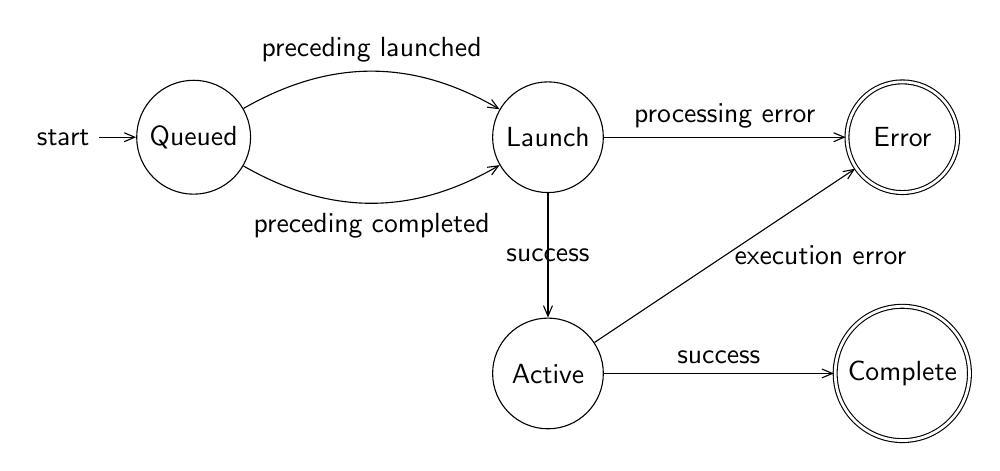
\begin{tikzpicture}
[auto,on grid,node distance=4.5cm,state/.style={circle,draw,minimum size=40pt}]
   \node[state,initial]                 (s0) {Queued};
   \node[state,right=4.5cm of s0]       (s1) {Launch};
   \node[state,below=3cm of s1]       (s2) {Active};
   \node[state,accepting,double distance=1pt,right=of s1]   (s3) {Error};
   \node[state,accepting,double distance=1pt,right=of s2]   (s4) {Complete};
   \path[->]
     (s0) edge[bend right]  node[below] {preceding completed} (s1)
          edge[bend left] node[above]{preceding launched} (s1)
     (s1) edge  node {processing error} (s3)
          edge  node[anchor=center] {success} (s2)
     (s2) edge  node{success} (s4)
          edge  node[right]{execution error} (s3)
     ;
\end{tikzpicture}
  \centering
  \caption{Packet State Diagram}
  \label{fig:packetstate}
\end{figure}

\begin{description}[leftmargin=0cm, labelindent=0cm]
\item[Queued] The format of the packet is not
  \hsaref{HSA_AQL_PACKET_FORMAT_ALWAYS_RESERVED} or
  \hsaref{HSA_AQL_PACKET_FORMAT_INVALID}. The transition to launch state occurs
  after all the preceding kernels have completed execution (if the
  \reffld{barrier} bit is set), or once they have completed their launch phase.

\item[Launch] The launch state implies processing of the packet, but not
  execution of a task. This phase finalizes by applying an acquire memory fence.
  If an error is detected during launch, the queue is set into an error state
  and the event callback associated with the queue (if present) is invoked. The
  following error might be communicated during the launch
  phase:\begin{inparaenum}[a\upshape)]\item
    \hsaref{HSA_STATUS_ERROR_INVALID_PACKET_FORMAT}, if the AQL packet is
    malformed\end{inparaenum}.

\item[Active] The kernel encoded by the packet starts executing. If an error is
  detected during this phase, a release fence is applied to the packet and its
  completion signal (if present) is assigned a negative value.

\item[Error] An error was encountered during the launch or active phases.

\item[Complete] A memory release fence is applied and the completion signal (if
  present) is decremented.
\end{description}

\subsubsection{Segment sizes}\label{segment-sizes}

If the kernel being dispatched uses private and group segments, the user is
required to specify the sizes of these segments in the dispatch
packet. Manually calculating this information is not feasible and requires
visual inspection of the user program, which itself may have been generated by a
higher-level compiler. Hence the user must rely on the finalizer to get the
corresponding segment sizes. Further details about determining segment sizes are
described in Section~\ref{finalizerchapter}.

Of the other HSA segments, the kernarg segment is also a part of the dispatch
packet, but as a pointer. This is because the kernarg segment carries the
arguments required to execute the kernel being dispatched and must be setup by
the user (the layout of this segment is language/finalization specific and
associated with the code object generated by finalization) prior to writing the
AQL packet to the queue (unlike the group and private segments, whose lifespan
spans only the active state of the dispatch packet). 
\subsection{Agent Dispatch packet}\label{agent-packet}

Agent Dispatch packets are used to dispatch jobs to HSA agents. In the HSA API,
they are of type \hsaref{hsa_aql_agent_dispatch_packet_t}. The set of states and
state transitions for agent dispatch packets is identical to that of dispatch
packets.

\subsection{Barrier packet}\label{barrier-packet}

The barrier packet \hsaref{hsa_aql_barrier_packet_t} allows the user to specify up to five dependencies as
\hsaref{hsa_signal_handle_t} objects and requires the packet processor to
resolve them before proceeding. The barrier packet is a blocking packet, in that
the processing of the barrier packet completes the packet and its completion
object is signaled. This is unlike a dispatch packet whose completion may occur
at some future time after the packet has finished processing.

If any of the dependent signals have been signaled with a negative value, the
barrier packet is complete, and will indicate failure in its completion
signal. The \reffld{completion_signal} will be signaled with the error value as
discussed in Section~\ref{sec:signals}. If the queue is not already in an error
state (e.g. the job generating the error was processed in a different queue)
then the packet processor should consider the error code on the dependent signal
to indicate an error in the queue itself and subsequently signal the
\reffld{error_signal} in the queue. When all of the dependent signals have been
signaled with the value 0, the \reffld{completion_signal} will be signaled with
the value 0 to indicate a successful completion.

The barrier packet also has a \reffld{barrier} bit that indicates that this
packet may only be processed when all previous packets have been marked as
completed.

The state diagram of the barrier packet is identical to that shown for dispatch
packets. However, each state might perform a different set of actions:
\begin{itemize}
\item No memory fence is applied in the launch phase.
\item In the active phase, instead of executing a kernel, the packet waits for
  all the conditions to be met. The following errors might be communicated
  during the active phase: \begin{inparaenum}[a\upshape)]\item
    \hsaref{HSA_STATUS_ERROR_SIGNAL_DEPENDENCY}, if an error is detected in one
    of the dependent signals (a negative value is observed).\end{inparaenum}
\item No action is performed in the completion phase.
\end{itemize}

\subsection{API}
\makeatletter{}

\noindent\begin{tcolorbox}[breakable,nobeforeafter,arc=0mm,colframe=white,colback=lightgray,left=0mm]
enum \hypertarget{group__aql_1ga21e03ac6edb26e457468af5fe501b7ad}{\textbf{hsa_aql_packet_format_t}}
\end{tcolorbox}
Packet type.

\noindent\textbf{Values}\\[-5mm]
\begin{longtable}{@{\hspace{2em}}p{\linewidth-2em}}
\hspace{-2em}\hypertarget{group__aql_1gga21e03ac6edb26e457468af5fe501b7adaaa022c87937de2531388a681182e4d36}{\refenu{HSA_AQL_PACKET_FORMAT_ALWAYS_RESERVED}} = 0\\Initial format of a packets when the queue is created. Always reserved packet have never been assigned to the packet processor. From a functional view always reserved packets are equivalent to invalid packets. All queues support this packet format.\\[2mm]
\hspace{-2em}\hypertarget{group__aql_1gga21e03ac6edb26e457468af5fe501b7adadc0bb64d5b0037718e716d57f6befb6a}{\refenu{HSA_AQL_PACKET_FORMAT_INVALID}} = 1\\The packet slot has been processed in the past, and has not been reassigned to the packet processor (is available). All queues support this packet format.\\[2mm]
\hspace{-2em}\hypertarget{group__aql_1gga21e03ac6edb26e457468af5fe501b7ada90d2a5dbd40f372f777402c83edf9d86}{\refenu{HSA_AQL_PACKET_FORMAT_DISPATCH}} = 2\\Packet used by HSA agents for dispatching jobs to HSA components. Not all queues support packets of this type (see \hyperlink{group__queue_1ga1145b01f6d9e2670179a22c92db39413}{hsa_queue_feature_t}).\\[2mm]
\hspace{-2em}\hypertarget{group__aql_1gga21e03ac6edb26e457468af5fe501b7adadaf10ccf48d374dfa87b7ad237a1788d}{\refenu{HSA_AQL_PACKET_FORMAT_BARRIER}} = 3\\Packet used by HSA agents to delay processing of subsequent packets, and to express complex dependencies between multiple packets. All queues support this packet format.\\[2mm]
\hspace{-2em}\hypertarget{group__aql_1gga21e03ac6edb26e457468af5fe501b7ada5189936e5f67be9e3463465aed69b008}{\refenu{HSA_AQL_PACKET_FORMAT_AGENT_DISPATCH}} = 4\\Packet used by HSA agents for dispatching jobs to HSA agents. Not all queues support packets of this type (see \hyperlink{group__queue_1ga1145b01f6d9e2670179a22c92db39413}{hsa_queue_feature_t}).
\end{longtable}

\noindent\begin{tcolorbox}[breakable,nobeforeafter,arc=0mm,colframe=white,colback=lightgray,left=0mm]
enum \hypertarget{group__aql_1ga6c1a86878de5b0f980202ad7e4e8d42a}{\textbf{hsa_fence_scope_t}}
\end{tcolorbox}
Scope of the memory fence operation associated with a packet.

\noindent\textbf{Values}\\[-5mm]
\begin{longtable}{@{\hspace{2em}}p{\linewidth-2em}}
\hspace{-2em}\hypertarget{group__aql_1gga6c1a86878de5b0f980202ad7e4e8d42aa5dc7b942cd56f91094a088435027be2c}{\refenu{HSA_FENCE_SCOPE_NONE}} = 0\\No scope. Only valid for barrier packets.\\[2mm]
\hspace{-2em}\hypertarget{group__aql_1gga6c1a86878de5b0f980202ad7e4e8d42aa9818589db02bc7c0639652eccd64c95d}{\refenu{HSA_FENCE_SCOPE_COMPONENT}} = 1\\The fence is applied with component scope for the global segment.\\[2mm]
\hspace{-2em}\hypertarget{group__aql_1gga6c1a86878de5b0f980202ad7e4e8d42aa6ecb203c10f12ec4bcf475d527c3a870}{\refenu{HSA_FENCE_SCOPE_SYSTEM}} = 2\\The fence is applied with system scope for the global segment.
\end{longtable}

\noindent\begin{tcolorbox}[breakable,nobeforeafter,arc=0mm,colframe=white,colback=lightgray,left=0mm]
typedef struct  hsa_aql_packet_header_s \{
\vspace{-3.5mm}\begin{longtable}{@{}p{\textwidth}}
\hspace{1.7em}\hyperlink{group__aql_1ga21e03ac6edb26e457468af5fe501b7ad}{hsa_aql_packet_format_t} \reffld{format} : 8;\\
\hspace{1.7em}uint16_t \reffld{barrier} : 1;\\
\hspace{1.7em}\hyperlink{group__aql_1ga6c1a86878de5b0f980202ad7e4e8d42a}{hsa_fence_scope_t} \reffld{acquire_fence_scope} : 2;\\
\hspace{1.7em}\hyperlink{group__aql_1ga6c1a86878de5b0f980202ad7e4e8d42a}{hsa_fence_scope_t} \reffld{release_fence_scope} : 2;\\
\hspace{1.7em}uint16_t \reffld{reserved} : 3;\\
\}  \hypertarget{group__aql_1ga92558e047d003985bae2558febd3dd40}{\textbf{hsa_aql_packet_header_t}}
\end{longtable}

\end{tcolorbox}
AQL packet header.

\noindent\textbf{Data Fields}\\[-6mm]
\begin{longtable}{@{}>{\hangindent=2em}p{\textwidth}}
\reffld{format}\\\hspace{2em}Packet type.\\[2mm]
\reffld{barrier}\\\hspace{2em}If set then processing of packets will only begin when all preceding packets are complete.\\[2mm]
\reffld{acquire_fence_scope}\\\hspace{2em}Determines the scope and type of the memory fence operation applied before the packet enters the active phase.\\[2mm]
\reffld{release_fence_scope}\\\hspace{2em}Determines the scope and type of the memory fence operation applied after kernel completion but before the packet is completed.\\[2mm]
\reffld{reserved}\\\hspace{2em}Must be zero.
\end{longtable}



\noindent\begin{tcolorbox}[breakable,nobeforeafter,arc=0mm,colframe=white,colback=lightgray,left=0mm]
typedef struct  hsa_aql_dispatch_packet_s \{
\vspace{-3.5mm}\begin{longtable}{@{}p{\textwidth}}
\hspace{1.7em}\hyperlink{group__aql_1ga92558e047d003985bae2558febd3dd40}{hsa_aql_packet_header_t} \reffld{header};\\
\hspace{1.7em}uint16_t \reffld{dimensions} : 2;\\
\hspace{1.7em}uint16_t \reffld{reserved} : 14;\\
\hspace{1.7em}uint16_t \reffld{workgroup_size_x};\\
\hspace{1.7em}uint16_t \reffld{workgroup_size_y};\\
\hspace{1.7em}uint16_t \reffld{workgroup_size_z};\\
\hspace{1.7em}uint16_t \reffld{reserved2};\\
\hspace{1.7em}uint32_t \reffld{grid_size_x};\\
\hspace{1.7em}uint32_t \reffld{grid_size_y};\\
\hspace{1.7em}uint32_t \reffld{grid_size_z};\\
\hspace{1.7em}uint32_t \reffld{private_segment_size_bytes};\\
\hspace{1.7em}uint32_t \reffld{group_segment_size_bytes};\\
\hspace{1.7em}uint64_t \reffld{kernel_object_address};\\
\hspace{1.7em}uint64_t \reffld{kernarg_address};\\
\hspace{1.7em}uint64_t \reffld{reserved3};\\
\hspace{1.7em}\hyperlink{group__signals_1ga6592c136d70853d855bc11d9efdbf534}{hsa_signal_handle_t} \reffld{completion_signal};\\
\}  \hypertarget{group__aql_1gab3d5ded5ac53f70931768468c0c0cfd6}{\textbf{hsa_aql_dispatch_packet_t}}
\end{longtable}

\end{tcolorbox}
AQL dispatch packet.

\noindent\textbf{Data Fields}\\[-6mm]
\begin{longtable}{@{}>{\hangindent=2em}p{\textwidth}}
\reffld{header}\\\hspace{2em}Packet header.\\[2mm]
\reffld{dimensions}\\\hspace{2em}Number of dimensions specified in the grid size. Valid values are 1,2, or 3.\\[2mm]
\reffld{reserved}\\\hspace{2em}Reserved, must be zero.\\[2mm]
\reffld{workgroup_size_x}\\\hspace{2em}X dimension of work-group (measured in work-items).\\[2mm]
\reffld{workgroup_size_y}\\\hspace{2em}Y dimension of work-group (measured in work-items).\\[2mm]
\reffld{workgroup_size_z}\\\hspace{2em}Z dimension of work-group (measured in work-items).\\[2mm]
\reffld{reserved2}\\\hspace{2em}Reserved. Must be zero.\\[2mm]
\reffld{grid_size_x}\\\hspace{2em}X dimension of grid (measured in work-items).\\[2mm]
\reffld{grid_size_y}\\\hspace{2em}Y dimension of grid (measured in work-items).\\[2mm]
\reffld{grid_size_z}\\\hspace{2em}Z dimension of grid (measured in work-items).\\[2mm]
\reffld{private_segment_size_bytes}\\\hspace{2em}Size (in bytes) of private memory allocation request (per work-item).\\[2mm]
\reffld{group_segment_size_bytes}\\\hspace{2em}Size (in bytes) of group memory allocation request (per work-group).\\[2mm]
\reffld{kernel_object_address}\\\hspace{2em}Address of an object in memory that includes an implementation-defined executable ISA image for the kernel.\\[2mm]
\reffld{kernarg_address}\\\hspace{2em}Address of memory containing kernel arguments.\\[2mm]
\reffld{reserved3}\\\hspace{2em}Reserved. Must be zero.\\[2mm]
\reffld{completion_signal}\\\hspace{2em}Signaling object handle used to indicate completion of the job.
\end{longtable}



\noindent\begin{tcolorbox}[breakable,nobeforeafter,arc=0mm,colframe=white,colback=lightgray,left=0mm]
typedef struct  hsa_aql_agent_dispatch_packet_s \{
\vspace{-3.5mm}\begin{longtable}{@{}p{\textwidth}}
\hspace{1.7em}\hyperlink{group__aql_1ga92558e047d003985bae2558febd3dd40}{hsa_aql_packet_header_t} \reffld{header};\\
\hspace{1.7em}uint16_t \reffld{type};\\
\hspace{1.7em}uint32_t \reffld{reserved2};\\
\hspace{1.7em}uint64_t \reffld{return_location};\\
\hspace{1.7em}uint64_t \reffld{arg}[4];\\
\hspace{1.7em}uint64_t \reffld{reserved3};\\
\hspace{1.7em}\hyperlink{group__signals_1ga6592c136d70853d855bc11d9efdbf534}{hsa_signal_handle_t} \reffld{completion_signal};\\
\}  \hypertarget{group__aql_1ga07dc7a6c787b5bee6e3f0b8b79586109}{\textbf{hsa_aql_agent_dispatch_packet_t}}
\end{longtable}

\end{tcolorbox}
Agent dispatch packet.

\noindent\textbf{Data Fields}\\[-6mm]
\begin{longtable}{@{}>{\hangindent=2em}p{\textwidth}}
\reffld{header}\\\hspace{2em}Packet header.\\[2mm]
\reffld{type}\\\hspace{2em}The function to be performed by the destination HSA Agent. The type value is split into the following ranges: 0x0000:0x3FFF (vendor specific), 0x4000:0x7FFF (HSA runtime) 0x8000:0xFFFF (user registered function).\\[2mm]
\reffld{reserved2}\\\hspace{2em}Reserved. Must be 0.\\[2mm]
\reffld{return_location}\\\hspace{2em}Pointer to location to store the function return value(s) in.\\[2mm]
\reffld{arg}\\\hspace{2em}64-bit direct or indirect arguments.\\[2mm]
\reffld{reserved3}\\\hspace{2em}Reserved. Must be 0.\\[2mm]
\reffld{completion_signal}\\\hspace{2em}Signaling object handle used to indicate completion of the job.
\end{longtable}



\noindent\begin{tcolorbox}[breakable,nobeforeafter,arc=0mm,colframe=white,colback=lightgray,left=0mm]
typedef struct  hsa_aql_barrier_packet_s \{
\vspace{-3.5mm}\begin{longtable}{@{}p{\textwidth}}
\hspace{1.7em}\hyperlink{group__aql_1ga92558e047d003985bae2558febd3dd40}{hsa_aql_packet_header_t} \reffld{header};\\
\hspace{1.7em}uint16_t \reffld{reserved2};\\
\hspace{1.7em}uint32_t \reffld{reserved3};\\
\hspace{1.7em}\hyperlink{group__signals_1ga6592c136d70853d855bc11d9efdbf534}{hsa_signal_handle_t} \reffld{dep_signal}[5];\\
\hspace{1.7em}uint64_t \reffld{reserved4};\\
\hspace{1.7em}\hyperlink{group__signals_1ga6592c136d70853d855bc11d9efdbf534}{hsa_signal_handle_t} \reffld{completion_signal};\\
\}  \hypertarget{group__aql_1ga8e5ebbeffbf5af1ece8db9ef27c14715}{\textbf{hsa_aql_barrier_packet_t}}
\end{longtable}

\end{tcolorbox}
Barrier packet.

\noindent\textbf{Data Fields}\\[-6mm]
\begin{longtable}{@{}>{\hangindent=2em}p{\textwidth}}
\reffld{header}\\\hspace{2em}Packet header.\\[2mm]
\reffld{reserved2}\\\hspace{2em}Reserved. Must be zero.\\[2mm]
\reffld{reserved3}\\\hspace{2em}Reserved. Must be zero.\\[2mm]
\reffld{dep_signal}\\\hspace{2em}Array of dependent signal objects.\\[2mm]
\reffld{reserved4}\\\hspace{2em}Reserved. Must be zero.\\[2mm]
\reffld{completion_signal}\\\hspace{2em}Signaling object handle used to indicate completion of the job.
\end{longtable}

 

\section{Memory}\label{memory}\hypertarget{memory}{}

One of the key features of HSA is its ability to share global pointers between
the host application and code executing on the component. This ability means
that an application can directly pass a pointer to memory allocated on the host
to a kernel function dispatched to a component without an intermediate copy.

\hypertarget{memory-registration}{}\subsection{Registration}\label{memory-registration}

When a buffer will be accessed by a kernel running on a HSA device, programmers
are encouraged to register the corresponding address range beforehand by using
the appropriate HSA core API invocation. While kernels running on HSA devices
can access any valid system memory pointer allocated by means of standard
libraries (for example, malloc in the C language) without resorting to
registration, there might be a performance benefit from registering the buffer
with the HSA core component. When an HSA program no longer needs to access a
registered buffer in a device, the user should deregister that virtual address
range by using the appropriate HSA core API invocation.


\subsection{Global  Memory Allocation}\label{globalmemory}

While a HSA component is capable of accessing pageable system memory by
definition, for scenarios where wants memory allocated that has already been
registered (combine the allocation with memory registration), the HSA runtime
provides an interface, \hsaref{hsa_memory_allocate} to allocate memory that is
internally registered by the runtime:


\hypertarget{kernarg}{}\subsection{Kernarg Memory}\label{kernargmem}

The kernarg memory that AQL packet points to (see Section~\ref{sec:aql}) holds
information about any arguments required to execute AQL dispatch on a HSA
component. While any system memory may be used for kernarg memory,
implementation/platform specific optimizations are possible if HSA core runtime
provided API are utilized for allocating and copying to the allocated kernarg
memory.

\hypertarget{device-memory}{}\subsection{Component Local Memory}
\label{device-memory}

Component local memory is a memory type that is dedicated specifically for a
particular HSA component. This memory could provide higher bandwidth for
component access (than system memory) with the limitation that the host might
not be able to access it directly. HSA runtime provides a host interface to
allocate/deallocate and access component local memory. The user should not
register or deregister component local memory.

\subsection{API}
\makeatletter{}

\noindent\begin{tcolorbox}[breakable,nobeforeafter,colframe=white,colback=lightgray,left=0mm]
\hyperlink{group__status_1gad755322e7ff95456520e8abdbe90d225}{hsa_status_t} \hypertarget{group__memory_1gaa4d4efc5ba903ea29587392aa1c8a267}{\textbf{hsa_memory_register}}(
\vspace{-3.5mm}\begin{longtable}{@{}p{\textwidth}}
\hspace{1.7em}void * \hsaarg{address},\\
\hspace{1.7em}size_t \hsaarg{size})\end{longtable}

\end{tcolorbox}
Register memory.

\noindent\textbf{Parameters}\\[-6mm]
\noindent\begin{longtable}{@{}>{\hangindent=2em}p{\textwidth}}
\hsaarg{address}\\\hspace{2em}(in) A pointer to the base of the memory region to be registered. If a null pointer is passed, no operation is performed.\\[2mm]
\hsaarg{size}\\\hspace{2em}(in) Requested registration size in bytes. If a size of zero is passed, no operation is performed.
\end{longtable}
\vspace{-5mm}\noindent\textbf{Return Values}\\[-6mm]
\noindent\begin{longtable}{@{}>{\hangindent=2em}p{\linewidth}}
\hyperlink{group__status_1ggad755322e7ff95456520e8abdbe90d225ae382ea0c9c05cce5a60d0317375159cc}{HSA_STATUS_SUCCESS}\\\hspace{2em}The function has been executed successfully.\\[2mm]
\hyperlink{group__status_1ggad755322e7ff95456520e8abdbe90d225a34ea59ade5bfce95eee935238a99f5b5}{HSA_STATUS_ERROR_NOT_INITIALIZED}\\\hspace{2em}The runtime has not been initialized.\\[2mm]
\hyperlink{group__status_1ggad755322e7ff95456520e8abdbe90d225a1a77fcf36d0d140874c4361ab093eff7}{HSA_STATUS_ERROR_OUT_OF_RESOURCES}\\\hspace{2em}If there is a failure in allocating the necessary resources.
\end{longtable}
\vspace{-4mm}\noindent\textbf{Description}\\[1mm]
Registering a system memory region for use with all the available devices This is an optional interface that is solely provided as a performance optimization hint to the underlying implementation so it may prepare for the future use of the memory by the devices. The interface is only beneficial for system memory that will be directly accessed by a device.\\[2mm]
Overlapping registrations are allowed. This is neither detrimental nor beneficial. 


\noindent\begin{tcolorbox}[breakable,nobeforeafter,colframe=white,colback=lightgray,left=0mm]
\hyperlink{group__status_1gad755322e7ff95456520e8abdbe90d225}{hsa_status_t} \hypertarget{group__memory_1ga05508ed130cdd83aeab76db3328a45fc}{\textbf{hsa_memory_deregister}}(
\vspace{-3.5mm}\begin{longtable}{@{}p{\textwidth}}
\hspace{1.7em}void * \hsaarg{address})\end{longtable}

\end{tcolorbox}
Deregister memory.

\noindent\textbf{Parameters}\\[-6mm]
\noindent\begin{longtable}{@{}>{\hangindent=2em}p{\textwidth}}
\hsaarg{address}\\\hspace{2em}(in) A pointer to the base of the memory region to be deregistered. If a NULL pointer is passed, no operation is performed.
\end{longtable}
\vspace{-5mm}\noindent\textbf{Return Values}\\[-6mm]
\noindent\begin{longtable}{@{}>{\hangindent=2em}p{\linewidth}}
\hyperlink{group__status_1ggad755322e7ff95456520e8abdbe90d225ae382ea0c9c05cce5a60d0317375159cc}{HSA_STATUS_SUCCESS}\\\hspace{2em}The function has been executed successfully.\\[2mm]
\hyperlink{group__status_1ggad755322e7ff95456520e8abdbe90d225a8b2f486dd206aa5545e8b0f2c1e2a568}{HSA_STATUS_ERROR_NOT_REGISTERED}\\\hspace{2em}If the pointer has not been registered before.
\end{longtable}
\vspace{-4mm}\noindent\textbf{Description}\\[1mm]
Used for deregistering a memory region previously registered.\\[2mm]
Deregistration must be performed using an address that was previously registered. In the event that deregistration is performed on an address that has been used in multiple registrations, the smallest of the registrations is deregistered. 


\noindent\begin{tcolorbox}[breakable,nobeforeafter,colframe=white,colback=lightgray,left=0mm]
\hyperlink{group__status_1gad755322e7ff95456520e8abdbe90d225}{hsa_status_t} \hypertarget{group__memory_1ga54b95840aafe4301a6c8cccea624f6e8}{\textbf{hsa_memory_allocate}}(
\vspace{-3.5mm}\begin{longtable}{@{}p{\textwidth}}
\hspace{1.7em}size_t \hsaarg{size_bytes},\\
\hspace{1.7em}void ** \hsaarg{address})\end{longtable}

\end{tcolorbox}
Allocate system memory.

\noindent\textbf{Parameters}\\[-6mm]
\noindent\begin{longtable}{@{}>{\hangindent=2em}p{\textwidth}}
\hsaarg{size_bytes}\\\hspace{2em}(in) Allocation size.\\[2mm]
\hsaarg{address}\\\hspace{2em}(in) Address pointer allocated by the user. Dereferenced and assigned to the pointer to the memory allocated for this request.
\end{longtable}
\vspace{-5mm}\noindent\textbf{Return Values}\\[-6mm]
\noindent\begin{longtable}{@{}>{\hangindent=2em}p{\linewidth}}
\hyperlink{group__status_1ggad755322e7ff95456520e8abdbe90d225ae382ea0c9c05cce5a60d0317375159cc}{HSA_STATUS_SUCCESS}\\\hspace{2em}The function has been executed successfully.\\[2mm]
\hyperlink{group__status_1ggad755322e7ff95456520e8abdbe90d225a34ea59ade5bfce95eee935238a99f5b5}{HSA_STATUS_ERROR_NOT_INITIALIZED}\\\hspace{2em}The runtime has not been initialized.\\[2mm]
\hyperlink{group__status_1ggad755322e7ff95456520e8abdbe90d225a1a77fcf36d0d140874c4361ab093eff7}{HSA_STATUS_ERROR_OUT_OF_RESOURCES}\\\hspace{2em}If there is a failure in allocation. This error may also occur when the core runtime library needs to spawn threads or create internal OS-specific events.\\[2mm]
\hyperlink{group__status_1ggad755322e7ff95456520e8abdbe90d225ac7d3651f75107d2a6a8ba3b25683c030}{HSA_STATUS_ERROR_INVALID_ARGUMENT}\\\hspace{2em}If the passed address is NULL.
\end{longtable}
\vspace{-4mm}\noindent\textbf{Description}\\[1mm]
The returned buffer is already registered. Allocation of size 0 is allowed and returns a NULL pointer. 


\noindent\begin{tcolorbox}[breakable,nobeforeafter,colframe=white,colback=lightgray,left=0mm]
\hyperlink{group__status_1gad755322e7ff95456520e8abdbe90d225}{hsa_status_t} \hypertarget{group__memory_1gaf968e8053981351ec0b16a04aeb51a8e}{\textbf{hsa_memory_free}}(
\vspace{-3.5mm}\begin{longtable}{@{}p{\textwidth}}
\hspace{1.7em}void * \hsaarg{ptr})\end{longtable}

\end{tcolorbox}
Free system memory.

\noindent\textbf{Parameters}\\[-6mm]
\noindent\begin{longtable}{@{}>{\hangindent=2em}p{\textwidth}}
\hsaarg{ptr}\\\hspace{2em}(in) Pointer to be released. If NULL, no action is performed
\end{longtable}
\vspace{-5mm}\noindent\textbf{Return Values}\\[-6mm]
\noindent\begin{longtable}{@{}>{\hangindent=2em}p{\linewidth}}
\hyperlink{group__status_1ggad755322e7ff95456520e8abdbe90d225ae382ea0c9c05cce5a60d0317375159cc}{HSA_STATUS_SUCCESS}\\\hspace{2em}The function has been executed successfully.\\[2mm]
\hyperlink{group__status_1ggad755322e7ff95456520e8abdbe90d225a34ea59ade5bfce95eee935238a99f5b5}{HSA_STATUS_ERROR_NOT_INITIALIZED}\\\hspace{2em}The runtime has not been initialized.
\end{longtable}
 


\noindent\begin{tcolorbox}[breakable,nobeforeafter,colframe=white,colback=lightgray,left=0mm]
\hyperlink{group__status_1gad755322e7ff95456520e8abdbe90d225}{hsa_status_t} \hypertarget{group__memory_1gaa26de25e2d7c7b8d96f5c2606d0b39a2}{\textbf{hsa_memory_allocate_kernarg}}(
\vspace{-3.5mm}\begin{longtable}{@{}p{\textwidth}}
\hspace{1.7em}const \hyperlink{group__topology_1gab8db3fb886332a24acac08ec361e1d86}{hsa_agent_t} * \hsaarg{component},\\
\hspace{1.7em}size_t \hsaarg{size},\\
\hspace{1.7em}void ** \hsaarg{address})\end{longtable}

\end{tcolorbox}
Allocate kernarg memory.

\noindent\textbf{Parameters}\\[-6mm]
\noindent\begin{longtable}{@{}>{\hangindent=2em}p{\textwidth}}
\hsaarg{component}\\\hspace{2em}(in) A valid pointer to the component for which the specified amount of kernarg memory is to be allocated.\\[2mm]
\hsaarg{size}\\\hspace{2em}(in) Requested allocation size in bytes. If size is 0, NULL is returned.\\[2mm]
\hsaarg{address}\\\hspace{2em}(out) A valid pointer to the location of where to return the pointer to the base of the allocated region of memory.
\end{longtable}
\vspace{-5mm}\noindent\textbf{Return Values}\\[-6mm]
\noindent\begin{longtable}{@{}>{\hangindent=2em}p{\linewidth}}
\hyperlink{group__status_1ggad755322e7ff95456520e8abdbe90d225ae382ea0c9c05cce5a60d0317375159cc}{HSA_STATUS_SUCCESS}\\\hspace{2em}The function has been executed successfully.\\[2mm]
\hyperlink{group__status_1ggad755322e7ff95456520e8abdbe90d225a34ea59ade5bfce95eee935238a99f5b5}{HSA_STATUS_ERROR_NOT_INITIALIZED}\\\hspace{2em}The runtime has not been initialized.\\[2mm]
\hyperlink{group__status_1ggad755322e7ff95456520e8abdbe90d225ac7d3651f75107d2a6a8ba3b25683c030}{HSA_STATUS_ERROR_INVALID_ARGUMENT}\\\hspace{2em}If the passed address is NULL.
\end{longtable}
 


\noindent\begin{tcolorbox}[breakable,nobeforeafter,colframe=white,colback=lightgray,left=0mm]
\hyperlink{group__status_1gad755322e7ff95456520e8abdbe90d225}{hsa_status_t} \hypertarget{group__memory_1gad585b1a966ffee1e0df23647de40237a}{\textbf{hsa_memory_free_kernarg}}(
\vspace{-3.5mm}\begin{longtable}{@{}p{\textwidth}}
\hspace{1.7em}void * \hsaarg{ptr})\end{longtable}

\end{tcolorbox}
Free kernarg memory.

\noindent\textbf{Parameters}\\[-6mm]
\noindent\begin{longtable}{@{}>{\hangindent=2em}p{\textwidth}}
\hsaarg{ptr}\\\hspace{2em}(in) Pointer to be released. If NULL, no action is performed
\end{longtable}
\vspace{-5mm}\noindent\textbf{Return Values}\\[-6mm]
\noindent\begin{longtable}{@{}>{\hangindent=2em}p{\linewidth}}
\hyperlink{group__status_1ggad755322e7ff95456520e8abdbe90d225ae382ea0c9c05cce5a60d0317375159cc}{HSA_STATUS_SUCCESS}\\\hspace{2em}The function has been executed successfully.\\[2mm]
\hyperlink{group__status_1ggad755322e7ff95456520e8abdbe90d225a34ea59ade5bfce95eee935238a99f5b5}{HSA_STATUS_ERROR_NOT_INITIALIZED}\\\hspace{2em}The runtime has not been initialized.
\end{longtable}
 


\noindent\begin{tcolorbox}[breakable,nobeforeafter,colframe=white,colback=lightgray,left=0mm]
\hyperlink{group__status_1gad755322e7ff95456520e8abdbe90d225}{hsa_status_t} \hypertarget{group__memory_1ga85b2081cde17a1bedd4027c196681be5}{\textbf{hsa_memory_copy_kernarg_to_system}}(
\vspace{-3.5mm}\begin{longtable}{@{}p{\textwidth}}
\hspace{1.7em}void * \hsaarg{dst},\\
\hspace{1.7em}const void * \hsaarg{src},\\
\hspace{1.7em}size_t \hsaarg{size})\end{longtable}

\end{tcolorbox}
Copy between the system and kernarg segments.

\noindent\textbf{Parameters}\\[-6mm]
\noindent\begin{longtable}{@{}>{\hangindent=2em}p{\textwidth}}
\hsaarg{dst}\\\hspace{2em}(out) A valid pointer to the destination array where the content is to be copied.\\[2mm]
\hsaarg{src}\\\hspace{2em}(in) A valid pointer to the source of data to be copied.\\[2mm]
\hsaarg{size}\\\hspace{2em}(in) Number of bytes to copy.
\end{longtable}
\vspace{-5mm}\noindent\textbf{Return Values}\\[-6mm]
\noindent\begin{longtable}{@{}>{\hangindent=2em}p{\linewidth}}
\hyperlink{group__status_1ggad755322e7ff95456520e8abdbe90d225ae382ea0c9c05cce5a60d0317375159cc}{HSA_STATUS_SUCCESS}\\\hspace{2em}The function has been executed successfully.\\[2mm]
\hyperlink{group__status_1ggad755322e7ff95456520e8abdbe90d225a34ea59ade5bfce95eee935238a99f5b5}{HSA_STATUS_ERROR_NOT_INITIALIZED}\\\hspace{2em}The runtime has not been initialized.\\[2mm]
\hyperlink{group__status_1ggad755322e7ff95456520e8abdbe90d225ac7d3651f75107d2a6a8ba3b25683c030}{HSA_STATUS_ERROR_INVALID_ARGUMENT}\\\hspace{2em}If the source or destination pointers are invalid.
\end{longtable}
 


\noindent\begin{tcolorbox}[breakable,nobeforeafter,colframe=white,colback=lightgray,left=0mm]
\hyperlink{group__status_1gad755322e7ff95456520e8abdbe90d225}{hsa_status_t} \hypertarget{group__memory_1ga34251efd3fcba21ab16c5c42eb27032f}{\textbf{hsa_memory_copy_system_to_kernarg}}(
\vspace{-3.5mm}\begin{longtable}{@{}p{\textwidth}}
\hspace{1.7em}void * \hsaarg{dst},\\
\hspace{1.7em}const void * \hsaarg{src},\\
\hspace{1.7em}size_t \hsaarg{size})\end{longtable}

\end{tcolorbox}
Copy between the system and kernarg segments.

\noindent\textbf{Parameters}\\[-6mm]
\noindent\begin{longtable}{@{}>{\hangindent=2em}p{\textwidth}}
\hsaarg{dst}\\\hspace{2em}(out) A valid pointer to the destination array where the content is to be copied.\\[2mm]
\hsaarg{src}\\\hspace{2em}(in) A valid pointer to the source of data to be copied.\\[2mm]
\hsaarg{size}\\\hspace{2em}(in) Number of bytes to copy.
\end{longtable}
\vspace{-5mm}\noindent\textbf{Return Values}\\[-6mm]
\noindent\begin{longtable}{@{}>{\hangindent=2em}p{\linewidth}}
\hyperlink{group__status_1ggad755322e7ff95456520e8abdbe90d225ae382ea0c9c05cce5a60d0317375159cc}{HSA_STATUS_SUCCESS}\\\hspace{2em}The function has been executed successfully.\\[2mm]
\hyperlink{group__status_1ggad755322e7ff95456520e8abdbe90d225a34ea59ade5bfce95eee935238a99f5b5}{HSA_STATUS_ERROR_NOT_INITIALIZED}\\\hspace{2em}The runtime has not been initialized.\\[2mm]
\hyperlink{group__status_1ggad755322e7ff95456520e8abdbe90d225ac7d3651f75107d2a6a8ba3b25683c030}{HSA_STATUS_ERROR_INVALID_ARGUMENT}\\\hspace{2em}If the source or destination pointers are invalid.
\end{longtable}
 


\noindent\begin{tcolorbox}[breakable,nobeforeafter,colframe=white,colback=lightgray,left=0mm]
\hyperlink{group__status_1gad755322e7ff95456520e8abdbe90d225}{hsa_status_t} \hypertarget{group__memory_1ga36a7f7550f61cfff55c566ee0ebc1be5}{\textbf{hsa_memory_allocate_component_local}}(
\vspace{-3.5mm}\begin{longtable}{@{}p{\textwidth}}
\hspace{1.7em}const \hyperlink{group__topology_1gab8db3fb886332a24acac08ec361e1d86}{hsa_agent_t} * \hsaarg{component},\\
\hspace{1.7em}size_t \hsaarg{size},\\
\hspace{1.7em}void ** \hsaarg{address})\end{longtable}

\end{tcolorbox}
Allocate memory on HSA Device.

\noindent\textbf{Parameters}\\[-6mm]
\noindent\begin{longtable}{@{}>{\hangindent=2em}p{\textwidth}}
\hsaarg{component}\\\hspace{2em}(in) A valid pointer to the HSA device for which the specified amount of global memory is to be allocated.\\[2mm]
\hsaarg{size}\\\hspace{2em}(in) Requested allocation size in bytes. If size is 0, NULL is returned.\\[2mm]
\hsaarg{address}\\\hspace{2em}(out) A valid pointer to the location of where to return the pointer to the base of the allocated region of memory.
\end{longtable}
\vspace{-5mm}\noindent\textbf{Return Values}\\[-6mm]
\noindent\begin{longtable}{@{}>{\hangindent=2em}p{\linewidth}}
\hyperlink{group__status_1ggad755322e7ff95456520e8abdbe90d225ae382ea0c9c05cce5a60d0317375159cc}{HSA_STATUS_SUCCESS}\\\hspace{2em}The function has been executed successfully.\\[2mm]
\hyperlink{group__status_1ggad755322e7ff95456520e8abdbe90d225a34ea59ade5bfce95eee935238a99f5b5}{HSA_STATUS_ERROR_NOT_INITIALIZED}\\\hspace{2em}The runtime has not been initialized.\\[2mm]
\hyperlink{group__status_1ggad755322e7ff95456520e8abdbe90d225a1a77fcf36d0d140874c4361ab093eff7}{HSA_STATUS_ERROR_OUT_OF_RESOURCES}\\\hspace{2em}If there is a failure in allocation of an internal structure required by the core runtime library. This error may also occur when the core runtime library needs to spawn threads or create internal OS-specific events.\\[2mm]
\hyperlink{group__status_1ggad755322e7ff95456520e8abdbe90d225ac7d3651f75107d2a6a8ba3b25683c030}{HSA_STATUS_ERROR_INVALID_ARGUMENT}\\\hspace{2em}If the passed component is NULL or invalid, or if the passed pointer is NULL.
\end{longtable}
\vspace{-4mm}\noindent\textbf{Description}\\[1mm]
Allocate global device memory associated with specified device. 


\noindent\begin{tcolorbox}[breakable,nobeforeafter,colframe=white,colback=lightgray,left=0mm]
\hyperlink{group__status_1gad755322e7ff95456520e8abdbe90d225}{hsa_status_t} \hypertarget{group__memory_1ga8f5353d063822f29295bddc230637817}{\textbf{hsa_memory_free_component_local}}(
\vspace{-3.5mm}\begin{longtable}{@{}p{\textwidth}}
\hspace{1.7em}void * \hsaarg{address})\end{longtable}

\end{tcolorbox}
Deallocate memory on HSA component.

\noindent\textbf{Parameters}\\[-6mm]
\noindent\begin{longtable}{@{}>{\hangindent=2em}p{\textwidth}}
\hsaarg{address}\\\hspace{2em}(in) A pointer to the address to be deallocated. If the pointer is NULL, no operation is performed.
\end{longtable}
\vspace{-5mm}\noindent\textbf{Return Values}\\[-6mm]
\noindent\begin{longtable}{@{}>{\hangindent=2em}p{\linewidth}}
\hyperlink{group__status_1ggad755322e7ff95456520e8abdbe90d225ae382ea0c9c05cce5a60d0317375159cc}{HSA_STATUS_SUCCESS}\\\hspace{2em}The function has been executed successfully.\\[2mm]
\hyperlink{group__status_1ggad755322e7ff95456520e8abdbe90d225a34ea59ade5bfce95eee935238a99f5b5}{HSA_STATUS_ERROR_NOT_INITIALIZED}\\\hspace{2em}The runtime has not been initialized.
\end{longtable}
\vspace{-4mm}\noindent\textbf{Description}\\[1mm]
Deallocate component memory that was allocated with \hyperlink{group__memory_1ga36a7f7550f61cfff55c566ee0ebc1be5}{\reffun{hsa_memory_allocate_component_local}}. 


\noindent\begin{tcolorbox}[breakable,nobeforeafter,colframe=white,colback=lightgray,left=0mm]
\hyperlink{group__status_1gad755322e7ff95456520e8abdbe90d225}{hsa_status_t} \hypertarget{group__memory_1ga292a4a5210b402fbf4320197d1cd3264}{\textbf{hsa_memory_copy_component_local_to_system}}(
\vspace{-3.5mm}\begin{longtable}{@{}p{\textwidth}}
\hspace{1.7em}void * \hsaarg{dst},\\
\hspace{1.7em}const void * \hsaarg{src},\\
\hspace{1.7em}size_t \hsaarg{size},\\
\hspace{1.7em}\hyperlink{group__signals_1ga6592c136d70853d855bc11d9efdbf534}{hsa_signal_handle_t} \hsaarg{signal})\end{longtable}

\end{tcolorbox}
Copy between the system and local heaps.

\noindent\textbf{Parameters}\\[-6mm]
\noindent\begin{longtable}{@{}>{\hangindent=2em}p{\textwidth}}
\hsaarg{dst}\\\hspace{2em}(out) A valid pointer to the destination array where the content is to be copied.\\[2mm]
\hsaarg{src}\\\hspace{2em}(in) A valid pointer to the source of data to be copied.\\[2mm]
\hsaarg{size}\\\hspace{2em}(in) Number of bytes to copy.\\[2mm]
\hsaarg{signal}\\\hspace{2em}(in) The signal that will be incremented by the runtime when the copy is complete.
\end{longtable}
\vspace{-5mm}\noindent\textbf{Return Values}\\[-6mm]
\noindent\begin{longtable}{@{}>{\hangindent=2em}p{\linewidth}}
\hyperlink{group__status_1ggad755322e7ff95456520e8abdbe90d225ae382ea0c9c05cce5a60d0317375159cc}{HSA_STATUS_SUCCESS}\\\hspace{2em}The function has been executed successfully.\\[2mm]
\hyperlink{group__status_1ggad755322e7ff95456520e8abdbe90d225a34ea59ade5bfce95eee935238a99f5b5}{HSA_STATUS_ERROR_NOT_INITIALIZED}\\\hspace{2em}The runtime has not been initialized.\\[2mm]
\hyperlink{group__status_1ggad755322e7ff95456520e8abdbe90d225a1a77fcf36d0d140874c4361ab093eff7}{HSA_STATUS_ERROR_OUT_OF_RESOURCES}\\\hspace{2em}If there is a failure in allocation of an internal structure required by the core runtime library. This error may also occur when the core runtime library needs to spawn threads or create internal OS-specific events.\\[2mm]
\hyperlink{group__status_1ggad755322e7ff95456520e8abdbe90d225ac7d3651f75107d2a6a8ba3b25683c030}{HSA_STATUS_ERROR_INVALID_ARGUMENT}\\\hspace{2em}If any argument is invalid.
\end{longtable}
 
 

\subsection{Example - memory registration}

A buffer is registered by indicating its starting address and a size. The size
does not need to match that of the original allocation. For example:

\begin{lstlisting}
void* ptr = malloc(16);
status = hsa_memory_register(ptr, 8);
if(status == HSA_STATUS_ERROR_INVALID_ARGUMENT)
  handle_error(status);
\end{lstlisting}

is a valid program. On the other hand:

\begin{lstlisting}
void* ptr = malloc(16);
status = hsa_memory_register(ptr, 20);
if(status == HSA_STATUS_ERROR_INVALID_ARGUMENT)
  handle_error(status);
\end{lstlisting}

is not a valid program, because we are registering a range that spans several
allocations, or might not be entirely allocated.

Registrations can overlap previously registered intervals. A special case of
overlapped registrations is multiple registration. If the same interval is
registered several times with different sizes, the HSA core component will
select the maximum as the size of all the registrations. Therefore, the
following program:

\begin{lstlisting}
status = hsa_memory_register(ptr, 8);
if(status == HSA_STATUS_ERROR_INVALID_ARGUMENT)
  handle_error(status);
status = hsa_memory_register(ptr, 16);
if(status == HSA_STATUS_ERROR_INVALID_ARGUMENT)
  handle_error(status);
\end{lstlisting}

behaves identically to this program:

\begin{lstlisting}
hsa_memory_register(ptr, 16);
if(status == HSA_STATUS_ERROR_INVALID_ARGUMENT)
  handle_error(status);
hsa_memory_register(ptr, 16);
if(status == HSA_STATUS_ERROR_INVALID_ARGUMENT)
  handle_error(status);
\end{lstlisting}

While the described behavior might seem counter-intuitive, consider the
following scenario: A pointer is registered twice with different sizes s1 and
s2. When the pointer is deregistered, which interval should be deregistered: (p,
s1) or (p, s2)? If all the registrations of the same pointer are considered
identical by the core runtime, that problem is eliminated.

Deregistering a pointer that has not been previously registered results in an
\emph{info} status indicating the same.

The following code snippet revisits the introductory example. The code is almost
identical to the original, except that we register the buffers that will be
accessed from the device after allocating them, and we deregister all that
memory before releasing it. In some platforms, we expect this version to perform
better than the original one.

\subsection{Example - device memory}
Component memory is allocated by indicating the size and the HSA device it
corresponds to. For example, the following code allocates 1024 bytes of device
local memory:

\begin{lstlisting}
void* component_ptr = NULL;
hsa_memory_allocate_component_local(1024, component, &component_ptr);
\end{lstlisting}

To access component memory from the host, the user can call
\hsaref{hsa_memory_copy_component_local_to_system} in similar fashion as in
memcpy. This interface allows the user to perform component-to-host memory
copy. For example:

\begin{lstlisting}
 const size_t DATA_SIZE = 1024;
 void* src_ptr = malloc(DATA_SIZE);
 void* dest_ptr = NULL;
 hsa_memory_allocate_component_local(DATA_SIZE, device, &dest_ptr);
 hsa_memory_copy_component_local_to_system(dest_ptr, src_ptr, DATA_SIZE);
\end{lstlisting}

copies 1024 bytes from system to component local memory.





\section{Extensions to the Core Runtime API}\label{extensions}

Extensions to the Core API can be optional (multi-vendor) or vendor
specific. The difference is in the naming scheme used for the symbols (defines,
structures, functions, etc.) associated with the function:

\begin{itemize}
\item Symbols for multi-vendor extensions defined in the global namespace must
  use the \emph{hsa_ext_} prefix in their identifiers.
\item Symbols for single vendor extensions defined in the global namespace must
  use the \emph{hsa_svext_VENDOR_} prefix in their identifiers. Company names
  must be registered with the HSA Foundation, must be unique, and may be
  abbreviated to improve the readability of the symbols.
\end{itemize}

Any constant definitions in the extension (\#define or enumeration values) use
the same naming convention, except using all capital letters.

The symbols for all vendor extensions (both single-vendor and multi-vendor) are
captured in the file {\bf hsa/vendor_extensions.h}. This file is maintained by
the HSA Foundation. This file includes the enumeration \hsaref{hsa_extension_t}
which defines a unique code for each vendor extension and multi-vendor
extension. Vendors can reserve enumeration encodings through the HSA
Foundation. Multi-vendor enumerations begin at the value of
\hsaref{HSA_EXT_START}, while single-vendor enumerations begin at
\hsaref{HSA_SVEXT_START}

\subsection{API}
\makeatletter{}

\noindent\begin{tcolorbox}[breakable,nobeforeafter,arc=0mm,colframe=white,colback=lightgray,left=0mm]
enum \hypertarget{group__extensions_1ga6a8dade2a7681dbd98a88029b1dbb5f3}{\textbf{hsa_extension_t}}
\end{tcolorbox}
HSA extensions.

\noindent\textbf{Values}\\[-5mm]
\begin{longtable}{@{\hspace{2em}}p{\linewidth-2em}}
\hspace{-2em}\hypertarget{group__extensions_1gga6a8dade2a7681dbd98a88029b1dbb5f3aac4cd309e9f72222b33b9c39cedf59b6}{\refenu{HSA_EXT_START}} = 0\\Start of the multi vendor extension range.\\[2mm]
\hspace{-2em}\hypertarget{group__extensions_1gga6a8dade2a7681dbd98a88029b1dbb5f3a2ca4542cee2ee2bcbc488b55267fd95b}{\refenu{HSA_EXT_FINALIZER}} = HSA_EXT_START\\Finalizer extension. Finalizes the brig to compilation units that represent kernel and function code objects.\\[2mm]
\hspace{-2em}\hypertarget{group__extensions_1gga6a8dade2a7681dbd98a88029b1dbb5f3a86fef6b16a18f71f235f9b8f7902b720}{\refenu{HSA_EXT_LINKER}} = 1\\Linker extension.\\[2mm]
\hspace{-2em}\hypertarget{group__extensions_1gga6a8dade2a7681dbd98a88029b1dbb5f3a7bafbcc066a693975751e025e47e52bc}{\refenu{HSA_EXT_IMAGES}} = 2\\Images extension.\\[2mm]
\hspace{-2em}\hypertarget{group__extensions_1gga6a8dade2a7681dbd98a88029b1dbb5f3a11513e66f5d7fce1a689cdccf8b9f08e}{\refenu{HSA_SVEXT_START}} = 10000\\Start of the single vendor extension range.
\end{longtable}

\noindent\begin{tcolorbox}[breakable,nobeforeafter,colframe=white,colback=lightgray,left=0mm]
\hyperlink{group__status_1gad755322e7ff95456520e8abdbe90d225}{hsa_status_t} \hypertarget{group__extensions_1ga87f219edc35dd68bb451a61f86fb1e18}{\textbf{hsa_vendor_extension_query}}(
\vspace{-3.5mm}\begin{longtable}{@{}p{\textwidth}}
\hspace{1.7em}\hyperlink{group__extensions_1ga6a8dade2a7681dbd98a88029b1dbb5f3}{hsa_extension_t} \hsaarg{extension},\\
\hspace{1.7em}void * \hsaarg{extension_structure},\\
\hspace{1.7em}int * \hsaarg{result})\end{longtable}

\end{tcolorbox}
Query vendor extensions.

\noindent\textbf{Parameters}\\[-6mm]
\noindent\begin{longtable}{@{}>{\hangindent=2em}p{\textwidth}}
\hsaarg{extension}\\\hspace{2em}(in) The vendor extension that is being queried.\\[2mm]
\hsaarg{extension_structure}\\\hspace{2em}(out) Extension structure.\\[2mm]
\hsaarg{result}\\\hspace{2em}(out) Pointer to memory location where to store the query result.
\end{longtable}
\vspace{-5mm}\noindent\textbf{Return Values}\\[-6mm]
\noindent\begin{longtable}{@{}>{\hangindent=2em}p{\linewidth}}
\hyperlink{group__status_1ggad755322e7ff95456520e8abdbe90d225ae382ea0c9c05cce5a60d0317375159cc}{HSA_STATUS_SUCCESS}\\\hspace{2em}The function has been executed successfully.\\[2mm]
\hyperlink{group__status_1ggad755322e7ff95456520e8abdbe90d225a34ea59ade5bfce95eee935238a99f5b5}{HSA_STATUS_ERROR_NOT_INITIALIZED}\\\hspace{2em}The runtime has not been initialized.\\[2mm]
\hyperlink{group__status_1ggad755322e7ff95456520e8abdbe90d225ac7d3651f75107d2a6a8ba3b25683c030}{HSA_STATUS_ERROR_INVALID_ARGUMENT}\\\hspace{2em}If \textit{extension} is not a valid value for a single vendor extension or \textit{result} is NULL.
\end{longtable}
\vspace{-4mm}\noindent\textbf{Description}\\[1mm]
If successful, the extension information is written with extension-specific information such as version information, function pointers, and data values. If the extension is not supported, the extension information is not modified. 


\noindent\begin{tcolorbox}[breakable,nobeforeafter,colframe=white,colback=lightgray,left=0mm]
\hyperlink{group__status_1gad755322e7ff95456520e8abdbe90d225}{hsa_status_t} \hypertarget{group__extensions_1ga7dd98c12faba2165267e7d072dee5859}{\textbf{hsa_extension_query}}(
\vspace{-3.5mm}\begin{longtable}{@{}p{\textwidth}}
\hspace{1.7em}\hyperlink{group__extensions_1ga6a8dade2a7681dbd98a88029b1dbb5f3}{hsa_extension_t} \hsaarg{extension},\\
\hspace{1.7em}int * \hsaarg{result})\end{longtable}

\end{tcolorbox}
Query HSA extensions.

\noindent\textbf{Parameters}\\[-6mm]
\noindent\begin{longtable}{@{}>{\hangindent=2em}p{\textwidth}}
\hsaarg{extension}\\\hspace{2em}(in) The extension that is being queried.\\[2mm]
\hsaarg{result}\\\hspace{2em}(out) Pointer to memory location where to store the query result.
\end{longtable}
\vspace{-5mm}\noindent\textbf{Return Values}\\[-6mm]
\noindent\begin{longtable}{@{}>{\hangindent=2em}p{\linewidth}}
\hyperlink{group__status_1ggad755322e7ff95456520e8abdbe90d225ae382ea0c9c05cce5a60d0317375159cc}{HSA_STATUS_SUCCESS}\\\hspace{2em}The function has been executed successfully.\\[2mm]
\hyperlink{group__status_1ggad755322e7ff95456520e8abdbe90d225a34ea59ade5bfce95eee935238a99f5b5}{HSA_STATUS_ERROR_NOT_INITIALIZED}\\\hspace{2em}The runtime has not been initialized.\\[2mm]
\hyperlink{group__status_1ggad755322e7ff95456520e8abdbe90d225ac7d3651f75107d2a6a8ba3b25683c030}{HSA_STATUS_ERROR_INVALID_ARGUMENT}\\\hspace{2em}If \textit{extension} is not a valid value for a HSA extension or \textit{result} is NULL.
\end{longtable}
 
 

\subsection{Example}
An example that shows a hypothetical single-vendor extension ``Foo'' registered
by company ``ACME''. The example includes four defines and two API functions.
Note the use of the structure \reftyp{hsa_svext_acme_foo_t} and how this
interacts with the \hsaref{hsa_vendor_extension_query} API call.

\lstinputlisting{example/extension.c}

\section{Common Definitions}\label{sec:other}
\makeatletter{}

\noindent\begin{tcolorbox}[nobeforeafter,arc=0mm,colframe=white,colback=lightgray,left=0mm]
typedef uint8_t  \hypertarget{group__RuntimeCommon_1ga143c7c845aca213614c1d79b65c35a0c}{\textbf{hsa_powertwo8_t}}
\end{tcolorbox}
Value expressed as a power of two.
\\

\noindent\begin{tcolorbox}[breakable,nobeforeafter,arc=0mm,colframe=white,colback=lightgray,left=0mm]
enum \hypertarget{group__RuntimeCommon_1ga45e8c4edc00ad0dc2c9e6e14e8610977}{\textbf{hsa_powertwo_t}}
\end{tcolorbox}
Power of two between 1 and 256.

\noindent\textbf{Values}\\[-5mm]
\begin{longtable}{@{\hspace{2em}}p{\linewidth-2em}}
\hspace{-2em}\hypertarget{group__RuntimeCommon_1gga45e8c4edc00ad0dc2c9e6e14e8610977a13bfa83a83c0f555efe4bbcca6b9cddf}{\refenu{HSA_POWERTWO_1}} = 0\\[2mm]
\hspace{-2em}\hypertarget{group__RuntimeCommon_1gga45e8c4edc00ad0dc2c9e6e14e8610977a465003dadda71ae8589097dd03202daf}{\refenu{HSA_POWERTWO_2}} = 1\\[2mm]
\hspace{-2em}\hypertarget{group__RuntimeCommon_1gga45e8c4edc00ad0dc2c9e6e14e8610977a04e128660c6aee9bd09b8be8683a4df9}{\refenu{HSA_POWERTWO_4}} = 2\\[2mm]
\hspace{-2em}\hypertarget{group__RuntimeCommon_1gga45e8c4edc00ad0dc2c9e6e14e8610977a6b602015c0db012f426e22c0354fbd05}{\refenu{HSA_POWERTWO_8}} = 3\\[2mm]
\hspace{-2em}\hypertarget{group__RuntimeCommon_1gga45e8c4edc00ad0dc2c9e6e14e8610977abc59007bbaea149704bb50a1aa70b7aa}{\refenu{HSA_POWERTWO_16}} = 4\\[2mm]
\hspace{-2em}\hypertarget{group__RuntimeCommon_1gga45e8c4edc00ad0dc2c9e6e14e8610977af13ebd4aecb93fd78bee555d26ed62a7}{\refenu{HSA_POWERTWO_32}} = 5\\[2mm]
\hspace{-2em}\hypertarget{group__RuntimeCommon_1gga45e8c4edc00ad0dc2c9e6e14e8610977a93252b7ad8bdcbec33390212e8897bd5}{\refenu{HSA_POWERTWO_64}} = 6\\[2mm]
\hspace{-2em}\hypertarget{group__RuntimeCommon_1gga45e8c4edc00ad0dc2c9e6e14e8610977ae78a1c50ad98ae134e34186acd52174e}{\refenu{HSA_POWERTWO_128}} = 7\\[2mm]
\hspace{-2em}\hypertarget{group__RuntimeCommon_1gga45e8c4edc00ad0dc2c9e6e14e8610977ae774bb9d85b5f7f9968ab76e50c23a6b}{\refenu{HSA_POWERTWO_256}} = 8
\end{longtable}

\noindent\begin{tcolorbox}[breakable,nobeforeafter,arc=0mm,colframe=white,colback=lightgray,left=0mm]
typedef struct  hsa_dim3_s \{
\vspace{-3.5mm}\begin{longtable}{@{}p{\textwidth}}
\hspace{1.7em}uint32_t \reffld{x};\\
\hspace{1.7em}uint32_t \reffld{y};\\
\hspace{1.7em}uint32_t \reffld{z};\\
\}  \hypertarget{group__RuntimeCommon_1ga6f7883588491965c45382cd996351aa2}{\textbf{hsa_dim3_t}}
\end{longtable}

\end{tcolorbox}
Three-dimensional coordinate.

\noindent\textbf{Data Fields}\\[-6mm]
\begin{longtable}{@{}>{\hangindent=2em}p{\textwidth}}
\reffld{x}\\\hspace{2em}X dimension.\\[2mm]
\reffld{y}\\\hspace{2em}Y dimension.\\[2mm]
\reffld{z}\\\hspace{2em}Z dimension
\end{longtable}



\noindent\begin{tcolorbox}[breakable,nobeforeafter,arc=0mm,colframe=white,colback=lightgray,left=0mm]
enum \hypertarget{group__RuntimeCommon_1gaa7eb83c51012a3b6f016f7b3388964ef}{\textbf{hsa_dim_t}}
\end{tcolorbox}
Dimensions in a 3D space.

\noindent\textbf{Values}\\[-5mm]
\begin{longtable}{@{\hspace{2em}}p{\linewidth-2em}}
\hspace{-2em}\hypertarget{group__RuntimeCommon_1ggaa7eb83c51012a3b6f016f7b3388964efa5a172a4cf084b71b9bafd68eaf159efc}{\refenu{HSA_DIM_X}} = 0\\X dimension.\\[2mm]
\hspace{-2em}\hypertarget{group__RuntimeCommon_1ggaa7eb83c51012a3b6f016f7b3388964efa863557e1bf7f7ba4f7ac00527f214d0e}{\refenu{HSA_DIM_Y}} = 1\\Y dimension.\\[2mm]
\hspace{-2em}\hypertarget{group__RuntimeCommon_1ggaa7eb83c51012a3b6f016f7b3388964efaa2ea7a7aba09bb743508177f196d2983}{\refenu{HSA_DIM_Z}} = 2\\Z dimension.
\end{longtable}

\noindent\begin{tcolorbox}[breakable,nobeforeafter,arc=0mm,colframe=white,colback=lightgray,left=0mm]
typedef struct  hsa_runtime_caller_s \{
\vspace{-3.5mm}\begin{longtable}{@{}p{\textwidth}}
\hspace{1.7em}uint64_t \reffld{caller};\\
\}  \hypertarget{group__RuntimeCommon_1ga7d9b1191602415f5dd3893985cc93826}{\textbf{hsa_runtime_caller_t}}
\end{longtable}

\end{tcolorbox}
Opaque pointer which is passed to all runtime functions that use callbacks. It is passed as the first argument to all callbacks made by the function.

\noindent\textbf{Data Fields}\\[-6mm]
\begin{longtable}{@{}>{\hangindent=2em}p{\textwidth}}
\reffld{caller}\\\hspace{2em}Opaque pointer which is passed as the first argument to callback functions invoked by a runtime function.
\end{longtable}



\noindent\begin{tcolorbox}[nobeforeafter,arc=0mm,colframe=white,colback=lightgray,left=0mm]
typedef \hyperlink{group__status_1gad755322e7ff95456520e8abdbe90d225}{hsa_status_t}(*  \hypertarget{group__RuntimeCommon_1ga30804c05fe32b4ab9da480280dba8cc5}{\textbf{hsa_runtime_alloc_data_callback_t}})(\hyperlink{group__RuntimeCommon_1ga7d9b1191602415f5dd3893985cc93826}{hsa_runtime_caller_t} caller, size_t byte_size, void **address)
\end{tcolorbox}
Call back function for allocating data.
\\ 


\chapter{HSA Extensions Programming Guide}

\section{HSAIL Finalization}
\label{finalizerchapter} \hypertarget{finalizerchapter}{}

The following subsections have to be updated according to the API definitions
introduced in version 0.180 of the specification.















































\subsubsection{API}
\makeatletter{}

\noindent\begin{tcolorbox}[nobeforeafter,arc=0mm,colframe=white,colback=lightgray,left=0mm]
typedef uint8_t  \hypertarget{group__FinalizerCoreApi_1ga4d058e43da41c147915dbe70cace9947}{\textbf{hsa_ext_brig_profile8_t}}
\end{tcolorbox}
BrigProfile is used to specify the kind of profile. This controls what features of HSAIL are supported. For more information see HSA Programmer's Reference Manual.
\\

\noindent\begin{tcolorbox}[breakable,nobeforeafter,arc=0mm,colframe=white,colback=lightgray,left=0mm]
enum \hypertarget{group__FinalizerCoreApi_1gaf65d6aea5a7200a4300f65306c08ea6e}{\textbf{hsa_ext_brig_profile_t}}
\end{tcolorbox}
BRIG profile values.

\noindent\textbf{Values}\\[-5mm]
\begin{longtable}{@{\hspace{2em}}p{\linewidth-2em}}
\hspace{-2em}\hypertarget{group__FinalizerCoreApi_1ggaf65d6aea5a7200a4300f65306c08ea6eadf0f501825c2f687f94fba6c2288d563}{\refenu{HSA_EXT_BRIG_PROFILE_BASE}} = 0\\Base profile.\\[2mm]
\hspace{-2em}\hypertarget{group__FinalizerCoreApi_1ggaf65d6aea5a7200a4300f65306c08ea6ea89285e7d3e3f19217df4e8f987c4126c}{\refenu{HSA_EXT_BRIG_PROFILE_FULL}} = 1\\Full profile.
\end{longtable}

\noindent\begin{tcolorbox}[nobeforeafter,arc=0mm,colframe=white,colback=lightgray,left=0mm]
typedef uint8_t  \hypertarget{group__FinalizerCoreApi_1ga5030b76e1c72556f42a7dc7eebab16df}{\textbf{hsa_ext_brig_machine_model8_t}}
\end{tcolorbox}
Machine model type. This controls the size of addresses used for segment and flat addresses. For more information see HSA Programmer's Reference Manual.
\\

\noindent\begin{tcolorbox}[breakable,nobeforeafter,arc=0mm,colframe=white,colback=lightgray,left=0mm]
enum \hypertarget{group__FinalizerCoreApi_1ga2079a73d7b54be5bb13026bac890dcbc}{\textbf{hsa_ext_brig_machine_model_t}}
\end{tcolorbox}
BRIG machine model.

\noindent\textbf{Values}\\[-5mm]
\begin{longtable}{@{\hspace{2em}}p{\linewidth-2em}}
\hspace{-2em}\hypertarget{group__FinalizerCoreApi_1gga2079a73d7b54be5bb13026bac890dcbca4d88cee5853fe4b072890619202c5b56}{\refenu{HSA_EXT_BRIG_MACHINE_SMALL}} = 0\\Use 32 bit addresses for global segment and flat addresses.\\[2mm]
\hspace{-2em}\hypertarget{group__FinalizerCoreApi_1gga2079a73d7b54be5bb13026bac890dcbca1d8a69a16cc565b2427ca590400081ef}{\refenu{HSA_EXT_BRIG_MACHINE_LARGE}} = 1\\Use 64 bit addresses for global segment and flat addresses.
\end{longtable}

\noindent\begin{tcolorbox}[nobeforeafter,arc=0mm,colframe=white,colback=lightgray,left=0mm]
typedef uint32_t  \hypertarget{group__FinalizerCoreApi_1ga2b753bccbe39c51384d6fa31a2302f0c}{\textbf{hsa_ext_brig_section_id32_t}}
\end{tcolorbox}
BRIG section id. The index into the array of sections in a BRIG module.
\\

\noindent\begin{tcolorbox}[breakable,nobeforeafter,arc=0mm,colframe=white,colback=lightgray,left=0mm]
enum \hypertarget{group__FinalizerCoreApi_1ga3060576486841364f0842a76810aea06}{\textbf{hsa_ext_brig_section_id_t}}
\end{tcolorbox}
The fixed BRIG sections ID of the predefined BRIG sections.

\noindent\textbf{Values}\\[-5mm]
\begin{longtable}{@{\hspace{2em}}p{\linewidth-2em}}
\hspace{-2em}\hypertarget{group__FinalizerCoreApi_1gga3060576486841364f0842a76810aea06a9b040e9aae3efa23134666d054a3a839}{\refenu{HSA_EXT_BRIG_SECTION_DATA}} = 0\\Data section, containing all character strings and byte data used in the finalization unit.\\[2mm]
\hspace{-2em}\hypertarget{group__FinalizerCoreApi_1gga3060576486841364f0842a76810aea06a43997c8d8ab6c03c301c949bdb1819c7}{\refenu{HSA_EXT_BRIG_SECTION_CODE}} = 1\\All of the executable operations. Most operations contain offsets to the .operand section.\\[2mm]
\hspace{-2em}\hypertarget{group__FinalizerCoreApi_1gga3060576486841364f0842a76810aea06ae52428f823f64d4ad9a0d8e2e29aea0b}{\refenu{HSA_EXT_BRIG_SECTION_OPERAND}} = 2\\The operands, such as immediate constants, registers, and address expressions, that appear in the operations.
\end{longtable}

\noindent\begin{tcolorbox}[breakable,nobeforeafter,arc=0mm,colframe=white,colback=lightgray,left=0mm]
typedef struct  hsa_ext_brig_section_header_s \{
\vspace{-3.5mm}\begin{longtable}{@{}p{\textwidth}}
\hspace{1.7em}uint32_t \reffld{byte_count};\\
\hspace{1.7em}uint32_t \reffld{header_byte_count};\\
\hspace{1.7em}uint32_t \reffld{name_length};\\
\hspace{1.7em}uint8_t \reffld{name}[1];\\
\}  \hypertarget{group__FinalizerCoreApi_1gaf9d6f363926d83463e8458aa5b5b0cf6}{\textbf{hsa_ext_brig_section_header_t}}
\end{longtable}

\end{tcolorbox}
BRIG section header. The first entry in every section must be this \hyperlink{group__FinalizerCoreApi_1gaf9d6f363926d83463e8458aa5b5b0cf6}{hsa_ext_brig_section_header_t} structure.

\noindent\textbf{Data Fields}\\[-6mm]
\begin{longtable}{@{}>{\hangindent=2em}p{\textwidth}}
\reffld{byte_count}\\\hspace{2em}Size in bytes of the section.\\[2mm]
\reffld{header_byte_count}\\\hspace{2em}Size of the header in bytes.\\[2mm]
\reffld{name_length}\\\hspace{2em}Length of \textit{name}\\[2mm]
\reffld{name}\\\hspace{2em}Dynamically sized section name.
\end{longtable}



\noindent\begin{tcolorbox}[breakable,nobeforeafter,arc=0mm,colframe=white,colback=lightgray,left=0mm]
typedef struct  hsa_ext_brig_module_s \{
\vspace{-3.5mm}\begin{longtable}{@{}p{\textwidth}}
\hspace{1.7em}uint32_t \reffld{section_count};\\
\hspace{1.7em}\hyperlink{group__FinalizerCoreApi_1gaf9d6f363926d83463e8458aa5b5b0cf6}{hsa_ext_brig_section_header_t} * \reffld{section}[1];\\
\}  \hypertarget{group__FinalizerCoreApi_1ga104477d24306200a2847b44c325e312a}{\textbf{hsa_ext_brig_module_t}}
\end{longtable}

\end{tcolorbox}
Top level BRIG module.

\noindent\textbf{Data Fields}\\[-6mm]
\begin{longtable}{@{}>{\hangindent=2em}p{\textwidth}}
\reffld{section_count}\\\hspace{2em}Number of sections in this BRIG module.\\[2mm]
\reffld{section}\\\hspace{2em}Sections in this BRIG module.
\end{longtable}



\noindent\begin{tcolorbox}[breakable,nobeforeafter,arc=0mm,colframe=white,colback=lightgray,left=0mm]
typedef struct  hsa_ext_brig_module_handle_s \{
\vspace{-3.5mm}\begin{longtable}{@{}p{\textwidth}}
\hspace{1.7em}uint64_t \reffld{handle};\\
\}  \hypertarget{group__FinalizerCoreApi_1ga0216996f5341a8591ecf9e0f6fd1b7e5}{\textbf{hsa_ext_brig_module_handle_t}}
\end{longtable}

\end{tcolorbox}
An opaque handle to the BRIG module.

\noindent\textbf{Data Fields}\\[-6mm]
\begin{longtable}{@{}>{\hangindent=2em}p{\textwidth}}
\reffld{handle}\\\hspace{2em}HSA component specific handle to the brig module.
\end{longtable}



\noindent\begin{tcolorbox}[nobeforeafter,arc=0mm,colframe=white,colback=lightgray,left=0mm]
typedef uint32_t  \hypertarget{group__FinalizerCoreApi_1ga494b8ac14a8c10af95b83b51a8a4ad7f}{\textbf{hsa_ext_brig_code_section_offset32_t}}
\end{tcolorbox}
BRIG code section offset.
\\

\noindent\begin{tcolorbox}[nobeforeafter,arc=0mm,colframe=white,colback=lightgray,left=0mm]
typedef uint16_t  \hypertarget{group__FinalizerCoreApi_1gaf05e7b6c47e7baac1cc9fb203047f168}{\textbf{hsa_ext_exception_kind16_t}}
\end{tcolorbox}
The set of exceptions supported by HSAIL. This is represented as a bit set.
\\

\noindent\begin{tcolorbox}[breakable,nobeforeafter,arc=0mm,colframe=white,colback=lightgray,left=0mm]
enum \hypertarget{group__FinalizerCoreApi_1gaac4b20de831dd17c83c1e2110bac0ef2}{\textbf{hsa_ext_exception_kind_t}}
\end{tcolorbox}
HSAIL exceptions.

\noindent\textbf{Values}\\[-5mm]
\begin{longtable}{@{\hspace{2em}}p{\linewidth-2em}}
\hspace{-2em}\hypertarget{group__FinalizerCoreApi_1ggaac4b20de831dd17c83c1e2110bac0ef2af3acf5b85fdfd50083ba20eb4142bb9f}{\refenu{HSA_EXT_EXCEPTION_INVALID_OPERATION}} = 1\\Operations are performed on values for which the results are not defined. These are:
\begin{itemize}\item Operations on signaling NaN (sNaN) floating-point values.
\item Signalling comparisons: comparisons on quiet NaN (qNaN) floating-point values.
\item Multiplication: mul(0.0, infinity) or mul(infinity, 0.0).
\item Fused multiply add: fma(0.0, infinity, c) or fma(infinity, 0.0, c) unless c is a quiet NaN, in which case it is implementation-defined if an exception is generated.
\item Addition, subtraction, or fused multiply add: magnitude subtraction of infinities, such as: add(positive infinity, negative infinity), sub(positive infinity, positive infinity).
\item Division: div(0.0, 0.0) or div(infinity, infinity).
\item Square root: sqrt(negative).
\item Conversion: A cvt with a floating-point source type, an integer destination type, and a nonsaturating rounding mode, when the source value is a NaN, infinity, or the rounded value, after any flush to zero, cannot be represented precisely in the integer type of the destination. 
\end{itemize}\\[2mm]
\hspace{-2em}\hypertarget{group__FinalizerCoreApi_1ggaac4b20de831dd17c83c1e2110bac0ef2adf54889632462cdeb6bbf4f36d0f630c}{\refenu{HSA_EXT_EXCEPTION_DIVIDE_BY_ZERO}} = 2\\A finite non-zero floating-point value is divided by zero. It is implementation defined if integer div or rem operations with a divisor of zero will generate a divide by zero exception.\\[2mm]
\hspace{-2em}\hypertarget{group__FinalizerCoreApi_1ggaac4b20de831dd17c83c1e2110bac0ef2a3cffa261ec9fbb0910b0ed11ea17126e}{\refenu{HSA_EXT_EXCEPTION_OVERFLOW}} = 4\\The floating-point exponent of a value is too large to be represented.\\[2mm]
\hspace{-2em}\hypertarget{group__FinalizerCoreApi_1ggaac4b20de831dd17c83c1e2110bac0ef2a15e11888d04953c37f86c8870807c888}{\refenu{HSA_EXT_EXCEPTION_UNDERFLOW}} = 8\\A non-zero tiny floating-point value is computed and either the ftz modifier is specified, or the ftz modifier was not specified and the value cannot be represented exactly.\\[2mm]
\hspace{-2em}\hypertarget{group__FinalizerCoreApi_1ggaac4b20de831dd17c83c1e2110bac0ef2ab0a718c671deb5e84e350199db22a24b}{\refenu{HSA_EXT_EXCEPTION_INEXACT}} = 16\\A computed floating-point value is not represented exactly in the destination. This can occur due to rounding. In addition, it is implementation defined if operations with the ftz modifier that cause a value to be flushed to zero generate the inexact exception.
\end{longtable}

\noindent\begin{tcolorbox}[nobeforeafter,arc=0mm,colframe=white,colback=lightgray,left=0mm]
typedef uint64_t  \hypertarget{group__FinalizerCoreApi_1ga366dea916dc7cec2954369e132e395e3}{\textbf{hsa_ext_control_directive_present64_t}}
\end{tcolorbox}
Bit set of control directives supported in HSAIL. See HSA Programmer's Reference Manual description of control directives with the same name for more information. For control directives that have an associated value, the value is given by the field in hsa_ext_control_directives_t. For control directives that are only present of absent (such as requirenopartialworkgroups) they have no corresponding field as the presence of the bit in this mask is sufficient.
\\

\noindent\begin{tcolorbox}[breakable,nobeforeafter,arc=0mm,colframe=white,colback=lightgray,left=0mm]
enum \hypertarget{group__FinalizerCoreApi_1ga143d9e622dfd7889d52fb5eb5ed1ffdb}{\textbf{hsa_ext_control_directive_present_t}}
\end{tcolorbox}
HSAIL control directives.

\noindent\textbf{Values}\\[-5mm]
\begin{longtable}{@{\hspace{2em}}p{\linewidth-2em}}
\hspace{-2em}\hypertarget{group__FinalizerCoreApi_1gga143d9e622dfd7889d52fb5eb5ed1ffdba1c209f3a9fd22b358006c221303f8893}{\refenu{HSA_EXT_CONTROL_DIRECTIVE_ENABLE_BREAK_EXCEPTIONS}} = 0\\If not enabled then must be 0, otherwise must be non-0 and specifies the set of HSAIL exceptions that must have the BREAK policy enabled. If this set is not empty then the generated code may have lower performance than if the set is empty. If the kernel being finalized has any enablebreakexceptions control directives, then the values specified by this argument are unioned with the values in these control directives. If any of the functions the kernel calls have an enablebreakexceptions control directive, then they must be equal or a subset of, this union.\\[2mm]
\hspace{-2em}\hypertarget{group__FinalizerCoreApi_1gga143d9e622dfd7889d52fb5eb5ed1ffdba5f6e061c9abd08976ee6f4c4ee48f30a}{\refenu{HSA_EXT_CONTROL_DIRECTIVE_ENABLE_DETECT_EXCEPTIONS}} = 1\\If not enabled then must be 0, otherwise must be non-0 and specifies the set of HSAIL exceptions that must have the DETECT policy enabled. If this set is not empty then the generated code may have lower performance than if the set is empty. However, an implementation should endeavour to make the performance impact small. If the kernel being finalized has any enabledetectexceptions control directives, then the values specified by this argument are unioned with the values in these control directives. If any of the functions the kernel calls have an enabledetectexceptions control directive, then they must be equal or a subset of, this union.\\[2mm]
\hspace{-2em}\hypertarget{group__FinalizerCoreApi_1gga143d9e622dfd7889d52fb5eb5ed1ffdba7787b99c887699ca6fe8d1cd4de3477e}{\refenu{HSA_EXT_CONTROL_DIRECTIVE_MAX_DYNAMIC_GROUP_SIZE}} = 2\\If not enabled then must be 0, and any amount of dynamic group segment can be allocated for a dispatch, otherwise the value specifies the maximum number of bytes of dynamic group segment that can be allocated for a dispatch. If the kernel being finalized has any maxdynamicsize control directives, then the values must be the same, and must be the same as this argument if it is enabled. This value can be used by the finalizer to determine the maximum number of bytes of group memory used by each work-group by adding this value to the group memory required for all group segment variables used by the kernel and all functions it calls, and group memory used to implement other HSAIL features such as fbarriers and the detect exception operations. This can allow the finalizer to determine the expected number of work-groups that can be executed by a compute unit and allow more resources to be allocated to the work-items if it is known that fewer work-groups can be executed due to group memory limitations.\\[2mm]
\hspace{-2em}\hypertarget{group__FinalizerCoreApi_1gga143d9e622dfd7889d52fb5eb5ed1ffdba8f84c9f5303be293df76bf82b002299c}{\refenu{HSA_EXT_CONTROL_DIRECTIVE_MAX_FLAT_GRID_SIZE}} = 4\\If not enabled then must be 0, otherwise must be greater than 0. Specifies the maximum number of work-items that will be in the grid when the kernel is dispatched. For more information see HSA Programmer's Reference Manual.\\[2mm]
\hspace{-2em}\hypertarget{group__FinalizerCoreApi_1gga143d9e622dfd7889d52fb5eb5ed1ffdbaa0e6d7d860284c6cadde5c7e9db66968}{\refenu{HSA_EXT_CONTROL_DIRECTIVE_MAX_FLAT_WORKGROUP_SIZE}} = 8\\If not enabled then must be 0, otherwise must be greater than 0. Specifies the maximum number of work-items that will be in the work-group when the kernel is dispatched. For more information see HSA Programmer's Reference Manual.\\[2mm]
\hspace{-2em}\hypertarget{group__FinalizerCoreApi_1gga143d9e622dfd7889d52fb5eb5ed1ffdbae6659470b66232e7ec4a749a032dc95d}{\refenu{HSA_EXT_CONTROL_DIRECTIVE_REQUESTED_WORKGROUPS_PER_CU}} = 16\\If not enabled then must be 0, and the finalizer is free to generate ISA that may result in any number of work-groups executing on a single compute unit. Otherwise, the finalizer should attempt to generate ISA that will allow the specified number of work-groups to execute on a single compute unit. This is only a hint and can be ignored by the finalizer. If the kernel being finalized, or any of the functions it calls, has a requested control directive, then the values must be the same. This can be used to determine the number of resources that should be allocated to a single work-group and work-item. For example, a low value may allow more resources to be allocated, resulting in higher per work-item performance, as it is known there will never be more than the specified number of work-groups actually executing on the compute unit. Conversely, a high value may allocate fewer resources, resulting in lower per work-item performance, which is offset by the fact it allows more work-groups to actually execute on the compute unit.\\[2mm]
\hspace{-2em}\hypertarget{group__FinalizerCoreApi_1gga143d9e622dfd7889d52fb5eb5ed1ffdbaa9878485a06df4090cba80c85acb32be}{\refenu{HSA_EXT_CONTROL_DIRECTIVE_REQUIRED_GRID_SIZE}} = 32\\If not enabled then all elements for Dim3 must be 0, otherwise every element must be greater than 0. Specifies the grid size that will be used when the kernel is dispatched. For more information see HSA Programmer's Reference Manual.\\[2mm]
\hspace{-2em}\hypertarget{group__FinalizerCoreApi_1gga143d9e622dfd7889d52fb5eb5ed1ffdbab26301028f39a1ac099aae9e74251438}{\refenu{HSA_EXT_CONTROL_DIRECTIVE_REQUIRED_WORKGROUP_SIZE}} = 64\\If not enabled then all elements for Dim3 must be 0, and the produced code can be dispatched with any legal work-group range consistent with the dispatch dimensions. Otherwise, the code produced must always be dispatched with the specified work-group range. No element of the specified range must be 0. It must be consistent with required_dimensions and max_flat_workgroup_size. If the kernel being finalized, or any of the functions it calls, has a requiredworkgroupsize control directive, then the values must be the same. Specifying a value can allow the finalizer to optimize work-group id operations, and if the number of work-items in the work-group is less tha the WAVESIZE then barrier operations can be optimized to just a memory fence.\\[2mm]
\hspace{-2em}\hypertarget{group__FinalizerCoreApi_1gga143d9e622dfd7889d52fb5eb5ed1ffdba87989d5d2c63b0bb44b15e0788bfe850}{\refenu{HSA_EXT_CONTROL_DIRECTIVE_REQUIRED_DIM}} = 128\\If not enabled then must be 0 and the produced kernel code can be dispatched with 1, 2 or 3 dimensions. If enabled then the value is 1..3 and the code produced must only be dispatched with a dimension that matches. Other values are illegal. If the kernel being finalized, or any of the functions it calls, has a requireddimsize control directive, then the values must be the same. This can be used to optimize the code generated to compute the absolute and flat work-group and work-item id, and the dim HSAIL operations.\\[2mm]
\hspace{-2em}\hypertarget{group__FinalizerCoreApi_1gga143d9e622dfd7889d52fb5eb5ed1ffdba5b5049bc2b376e60b9b92337e343ee18}{\refenu{HSA_EXT_CONTROL_DIRECTIVE_REQUIRE_NO_PARTIAL_WORKGROUPS}} = 256\\Specifies that the kernel must be dispatched with no partial work-groups. It can be placed in either a kernel or a function code block. This is only a hint and can be ignored by the finalizer.\\[2mm]
It is undefined if the kernel is dispatched with any dimension of the grid size not being an exact multiple of the corresponding dimension of the work-group size.\\[2mm]
A finalizer might be able to generate better code for currentworkgroupsize if it knows there are no partial work-groups, because the result becomes the same as the workgroupsize operation. An HSA component might be able to dispatch a kernel more efficiently if it knows there are no partial work-groups.\\[2mm]
The control directive applies to the whole kernel and all functions it calls. It can appear multiple times in a kernel or function. If it appears in a function (including external functions), then it must also appear in all kernels that call that function (or have been specified when the finalizer was invoked), either directly or indirectly.\\[2mm]
If require no partial work-groups is specified when the finalizer is invoked, the kernel behaves as if the requirenopartialworkgroups control directive has been specified.\\[2mm]
require_no_partial_work_groups does not have a field since having the bit set in enabledControlDirectives indicates that the cpntrol directive is present.
\end{longtable}

\noindent\begin{tcolorbox}[breakable,nobeforeafter,arc=0mm,colframe=white,colback=lightgray,left=0mm]
typedef struct  hsa_ext_control_directives_s \{
\vspace{-3.5mm}\begin{longtable}{@{}p{\textwidth}}
\hspace{1.7em}\hyperlink{group__FinalizerCoreApi_1ga366dea916dc7cec2954369e132e395e3}{hsa_ext_control_directive_present64_t} \reffld{enabled_control_directives};\\
\hspace{1.7em}\hyperlink{group__FinalizerCoreApi_1gaf05e7b6c47e7baac1cc9fb203047f168}{hsa_ext_exception_kind16_t} \reffld{enable_break_exceptions};\\
\hspace{1.7em}\hyperlink{group__FinalizerCoreApi_1gaf05e7b6c47e7baac1cc9fb203047f168}{hsa_ext_exception_kind16_t} \reffld{enable_detect_exceptions};\\
\hspace{1.7em}uint32_t \reffld{max_dynamic_group_size};\\
\hspace{1.7em}uint32_t \reffld{max_flat_grid_size};\\
\hspace{1.7em}uint32_t \reffld{max_flat_workgroup_size};\\
\hspace{1.7em}uint32_t \reffld{requested_workgroups_per_cu};\\
\hspace{1.7em}\hyperlink{group__RuntimeCommon_1ga6f7883588491965c45382cd996351aa2}{hsa_dim3_t} \reffld{required_grid_size};\\
\hspace{1.7em}\hyperlink{group__RuntimeCommon_1ga6f7883588491965c45382cd996351aa2}{hsa_dim3_t} \reffld{required_workgroup_size};\\
\hspace{1.7em}uint8_t \reffld{required_dim};\\
\hspace{1.7em}uint8_t \reffld{reserved}[75];\\
\}  \hypertarget{group__FinalizerCoreApi_1ga40c83573be6c1e21ad46ff8a7edd21b0}{\textbf{hsa_ext_control_directives_t}}
\end{longtable}

\end{tcolorbox}
The hsa_ext_control_directives_t specifies the values for the HSAIL control directives. These control how the finalizer generates code. This struct is used both as an argument to hsaFinalizeKernel to specify values for the control directives, and is used in HsaKernelCode to record the values of the control directives that the finalize used when generating the code which either came from the finalizer argument or explicit HSAIL control directives. See the definition of the control directives in HSA Programmer's Reference Manual which also defines how the values specified as finalizer arguments have to agree with the control directives in the HSAIL code.

\noindent\textbf{Data Fields}\\[-6mm]
\begin{longtable}{@{}>{\hangindent=2em}p{\textwidth}}
\reffld{enabled_control_directives}\\\hspace{2em}This is a bit set indicating which control directives have been specified. If the value is 0 then there are no control directives specified and the rest of the fields can be ignored. The bits are accessed using the hsa_ext_control_directives_present_mask_t. Any control directive that is not enabled in this bit set must have the value of all 0s.\\[2mm]
\reffld{enable_break_exceptions}\\\hspace{2em}If enableBreakExceptions is not enabled then must be 0, otherwise must be non-0 and specifies the set of HSAIL exceptions that must have the BREAK policy enabled. If this set is not empty then the generated code may have lower performance than if the set is empty. If the kernel being finalized has any enablebreakexceptions control directives, then the values specified by this argument are unioned with the values in these control directives. If any of the functions the kernel calls have an enablebreakexceptions control directive, then they must be equal or a subset of, this union.\\[2mm]
\reffld{enable_detect_exceptions}\\\hspace{2em}If enableDetectExceptions is not enabled then must be 0, otherwise must be non-0 and specifies the set of HSAIL exceptions that must have the DETECT policy enabled. If this set is not empty then the generated code may have lower performance than if the set is empty. However, an implementation should endeavour to make the performance impact small. If the kernel being finalized has any enabledetectexceptions control directives, then the values specified by this argument are unioned with the values in these control directives. If any of the functions the kernel calls have an enabledetectexceptions control directive, then they must be equal or a subset of, this union.\\[2mm]
\reffld{max_dynamic_group_size}\\\hspace{2em}If maxDynamicGroupSize is not enabled then must be 0, and any amount of dynamic group segment can be allocated for a dispatch, otherwise the value specifies the maximum number of bytes of dynamic group segment that can be allocated for a dispatch. If the kernel being finalized has any maxdynamicsize control directives, then the values must be the same, and must be the same as this argument if it is enabled. This value can be used by the finalizer to determine the maximum number of bytes of group memory used by each work-group by adding this value to the group memory required for all group segment variables used by the kernel and all functions it calls, and group memory used to implement other HSAIL features such as fbarriers and the detect exception operations. This can allow the finalizer to determine the expected number of work-groups that can be executed by a compute unit and allow more resources to be allocated to the work-items if it is known that fewer work-groups can be executed due to group memory limitations.\\[2mm]
\reffld{max_flat_grid_size}\\\hspace{2em}If maxFlatGridSize is not enabled then must be 0, otherwise must be greater than 0. See HSA Programmer's Reference Manual description of maxflatgridsize control directive.\\[2mm]
\reffld{max_flat_workgroup_size}\\\hspace{2em}If maxFlatWorkgroupSize is not enabled then must be 0, otherwise must be greater than 0. See HSA Programmer's Reference Manual description of maxflatworkgroupsize control directive.\\[2mm]
\reffld{requested_workgroups_per_cu}\\\hspace{2em}If requestedWorkgroupsPerCu is not enabled then must be 0, and the finalizer is free to generate ISA that may result in any number of work-groups executing on a single compute unit. Otherwise, the finalizer should attempt to generate ISA that will allow the specified number of work-groups to execute on a single compute unit. This is only a hint and can be ignored by the finalizer. If the kernel being finalized, or any of the functions it calls, has a requested control directive, then the values must be the same. This can be used to determine the number of resources that should be allocated to a single work-group and work-item. For example, a low value may allow more resources to be allocated, resulting in higher per work-item performance, as it is known there will never be more than the specified number of work-groups actually executing on the compute unit. Conversely, a high value may allocate fewer resources, resulting in lower per work-item performance, which is offset by the fact it allows more work-groups to actually execute on the compute unit.\\[2mm]
\reffld{required_grid_size}\\\hspace{2em}If not enabled then all elements for Dim3 must be 0, otherwise every element must be greater than 0. See HSA Programmer's Reference Manual description of requiredgridsize control directive.\\[2mm]
\reffld{required_workgroup_size}\\\hspace{2em}If requiredWorkgroupSize is not enabled then all elements for Dim3 must be 0, and the produced code can be dispatched with any legal work-group range consistent with the dispatch dimensions. Otherwise, the code produced must always be dispatched with the specified work-group range. No element of the specified range must be 0. It must be consistent with required_dimensions and max_flat_workgroup_size. If the kernel being finalized, or any of the functions it calls, has a requiredworkgroupsize control directive, then the values must be the same. Specifying a value can allow the finalizer to optimize work-group id operations, and if the number of work-items in the work-group is less than the WAVESIZE then barrier operations can be optimized to just a memory fence.\\[2mm]
\reffld{required_dim}\\\hspace{2em}If requiredDim is not enabled then must be 0 and the produced kernel code can be dispatched with 1, 2 or 3 dimensions. If enabled then the value is 1..3 and the code produced must only be dispatched with a dimension that matches. Other values are illegal. If the kernel being finalized, or any of the functions it calls, has a requireddimsize control directive, then the values must be the same. This can be used to optimize the code generated to compute the absolute and flat work-group and work-item id, and the dim HSAIL operations.\\[2mm]
\reffld{reserved}\\\hspace{2em}Reserved. Must be 0.
\end{longtable}



\noindent\begin{tcolorbox}[nobeforeafter,arc=0mm,colframe=white,colback=lightgray,left=0mm]
typedef uint32_t  \hypertarget{group__FinalizerCoreApi_1gaeb2b662521c2d1056eec8dfd45fbb960}{\textbf{hsa_ext_code_kind32_t}}
\end{tcolorbox}
The kinds of code objects that can be contained in \hyperlink{group__FinalizerCoreApi_1ga0e01eabc57d7105ea37e1abbb50fa337}{hsa_ext_code_descriptor_t}.
\\

\noindent\begin{tcolorbox}[breakable,nobeforeafter,arc=0mm,colframe=white,colback=lightgray,left=0mm]
enum \hypertarget{group__FinalizerCoreApi_1ga3a26aac857ef4f02699a2ed8a4c425e3}{\textbf{hsa_ext_code_kind_t}}
\end{tcolorbox}
Type of code object.

\noindent\textbf{Values}\\[-5mm]
\begin{longtable}{@{\hspace{2em}}p{\linewidth-2em}}
\hspace{-2em}\hypertarget{group__FinalizerCoreApi_1gga3a26aac857ef4f02699a2ed8a4c425e3aa692c691cdb10a56486a1e8d246414e3}{\refenu{HSA_EXT_CODE_NONE}} = 0\\Not a code object.\\[2mm]
\hspace{-2em}\hypertarget{group__FinalizerCoreApi_1gga3a26aac857ef4f02699a2ed8a4c425e3a5c83ef1db7eaa20cdf2612ba26e316cc}{\refenu{HSA_EXT_CODE_KERNEL}} = 1\\HSAIL kernel that can be used with an AQL dispatch packet.\\[2mm]
\hspace{-2em}\hypertarget{group__FinalizerCoreApi_1gga3a26aac857ef4f02699a2ed8a4c425e3a5f810d8ab0aae6b7f5af079857bbb14c}{\refenu{HSA_EXT_CODE_INDIRECT_FUNCTION}} = 2\\HSAIL indirect function.\\[2mm]
\hspace{-2em}\hypertarget{group__FinalizerCoreApi_1gga3a26aac857ef4f02699a2ed8a4c425e3afe329fae97936c684cd1e7df360c7160}{\refenu{HSA_EXT_CODE_RUNTIME_FIRST}} = 0x40000000\\HSA runtime code objects. For example, partially linked code objects.\\[2mm]
\hspace{-2em}\hypertarget{group__FinalizerCoreApi_1gga3a26aac857ef4f02699a2ed8a4c425e3a9c49857996a8d326eabb3080b9e38972}{\refenu{HSA_EXT_CODE_RUNTIME_LAST}} = 0x7fffffff\\[2mm]
\hspace{-2em}\hypertarget{group__FinalizerCoreApi_1gga3a26aac857ef4f02699a2ed8a4c425e3aefd6d814296d049b06ab2de301cd10b1}{\refenu{HSA_EXT_CODE_VENDOR_FIRST}} = 0x80000000\\Vendor specific code objects.\\[2mm]
\hspace{-2em}\hypertarget{group__FinalizerCoreApi_1gga3a26aac857ef4f02699a2ed8a4c425e3accaced1295912da1748d70c5abde593b}{\refenu{HSA_EXT_CODE_VENDOR_LAST}} = 0xffffffff
\end{longtable}

\noindent\begin{tcolorbox}[nobeforeafter,arc=0mm,colframe=white,colback=lightgray,left=0mm]
typedef uint32_t  \hypertarget{group__FinalizerCoreApi_1gad4afadfa0983f1bc637f3add3a006cba}{\textbf{hsa_ext_program_call_convention_id32_t}}
\end{tcolorbox}
Program call convention.
\\

\noindent\begin{tcolorbox}[breakable,nobeforeafter,arc=0mm,colframe=white,colback=lightgray,left=0mm]
enum \hypertarget{group__FinalizerCoreApi_1gad40f97fe8e2356f3a58c3073f12cf5ad}{\textbf{hsa_ext_program_call_convention_id_t}}
\end{tcolorbox}
Types of program call conventions.

\noindent\textbf{Values}\\[-5mm]
\begin{longtable}{@{\hspace{2em}}p{\linewidth-2em}}
\hspace{-2em}\hypertarget{group__FinalizerCoreApi_1ggad40f97fe8e2356f3a58c3073f12cf5ada644970a843ed5c5f6f48b524e42c95c3}{\refenu{HSA_EXT_PROGRAM_CALL_CONVENTION_FINALIZER_DETERMINED}} = -1
\end{longtable}

\noindent\begin{tcolorbox}[breakable,nobeforeafter,arc=0mm,colframe=white,colback=lightgray,left=0mm]
typedef struct  hsa_ext_code_handle_s \{
\vspace{-3.5mm}\begin{longtable}{@{}p{\textwidth}}
\hspace{1.7em}uint64_t \reffld{handle};\\
\}  \hypertarget{group__FinalizerCoreApi_1ga5aeece3297b7102d33a2815a368103f7}{\textbf{hsa_ext_code_handle_t}}
\end{longtable}

\end{tcolorbox}
An opaque handle to the code object.

\noindent\textbf{Data Fields}\\[-6mm]
\begin{longtable}{@{}>{\hangindent=2em}p{\textwidth}}
\reffld{handle}\\\hspace{2em}HSA component specific handle to the code.
\end{longtable}



\noindent\begin{tcolorbox}[breakable,nobeforeafter,arc=0mm,colframe=white,colback=lightgray,left=0mm]
typedef struct  hsa_ext_debug_information_handle_s \{
\vspace{-3.5mm}\begin{longtable}{@{}p{\textwidth}}
\hspace{1.7em}uint64_t \reffld{handle};\\
\}  \hypertarget{group__FinalizerCoreApi_1gaf4c0bece520460a2d77a9309905395f3}{\textbf{hsa_ext_debug_information_handle_t}}
\end{longtable}

\end{tcolorbox}
An opaque handle to the debug information.

\noindent\textbf{Data Fields}\\[-6mm]
\begin{longtable}{@{}>{\hangindent=2em}p{\textwidth}}
\reffld{handle}\\\hspace{2em}HSA component specific handle to the debug information.
\end{longtable}



\noindent\begin{tcolorbox}[breakable,nobeforeafter,arc=0mm,colframe=white,colback=lightgray,left=0mm]
typedef struct  hsa_ext_code_descriptor_s \{
\vspace{-3.5mm}\begin{longtable}{@{}p{\textwidth}}
\hspace{1.7em}\hyperlink{group__FinalizerCoreApi_1gaeb2b662521c2d1056eec8dfd45fbb960}{hsa_ext_code_kind32_t} \reffld{code_type};\\
\hspace{1.7em}uint32_t \reffld{workgroup_group_segment_byte_size};\\
\hspace{1.7em}uint64_t \reffld{kernarg_segment_byte_size};\\
\hspace{1.7em}uint32_t \reffld{workitem_private_segment_byte_size};\\
\hspace{1.7em}uint32_t \reffld{workgroup_fbarrier_count};\\
\hspace{1.7em}\hyperlink{group__FinalizerCoreApi_1ga5aeece3297b7102d33a2815a368103f7}{hsa_ext_code_handle_t} \reffld{code};\\
\hspace{1.7em}\hyperlink{group__RuntimeCommon_1ga143c7c845aca213614c1d79b65c35a0c}{hsa_powertwo8_t} \reffld{kernarg_segment_alignment};\\
\hspace{1.7em}\hyperlink{group__RuntimeCommon_1ga143c7c845aca213614c1d79b65c35a0c}{hsa_powertwo8_t} \reffld{group_segment_alignment};\\
\hspace{1.7em}\hyperlink{group__RuntimeCommon_1ga143c7c845aca213614c1d79b65c35a0c}{hsa_powertwo8_t} \reffld{private_segment_alignment};\\
\hspace{1.7em}\hyperlink{group__RuntimeCommon_1ga143c7c845aca213614c1d79b65c35a0c}{hsa_powertwo8_t} \reffld{wavefront_size};\\
\hspace{1.7em}\hyperlink{group__FinalizerCoreApi_1gad4afadfa0983f1bc637f3add3a006cba}{hsa_ext_program_call_convention_id32_t} \reffld{program_call_convention};\\
\hspace{1.7em}\hyperlink{group__FinalizerCoreApi_1ga0216996f5341a8591ecf9e0f6fd1b7e5}{hsa_ext_brig_module_handle_t} \reffld{module};\\
\hspace{1.7em}\hyperlink{group__FinalizerCoreApi_1ga494b8ac14a8c10af95b83b51a8a4ad7f}{hsa_ext_brig_code_section_offset32_t} \reffld{symbol};\\
\hspace{1.7em}\hyperlink{group__FinalizerCoreApi_1ga4d058e43da41c147915dbe70cace9947}{hsa_ext_brig_profile8_t} \reffld{hsail_profile};\\
\hspace{1.7em}\hyperlink{group__FinalizerCoreApi_1ga5030b76e1c72556f42a7dc7eebab16df}{hsa_ext_brig_machine_model8_t} \reffld{hsail_machine_model};\\
\hspace{1.7em}uint16_t \reffld{reserved1};\\
\hspace{1.7em}\hyperlink{group__FinalizerCoreApi_1gaf4c0bece520460a2d77a9309905395f3}{hsa_ext_debug_information_handle_t} \reffld{debug_information};\\
\hspace{1.7em}char \reffld{agent_vendor}[24];\\
\hspace{1.7em}char \reffld{agent_name}[24];\\
\hspace{1.7em}uint32_t \reffld{hsail_version_major};\\
\hspace{1.7em}uint32_t \reffld{hsail_version_minor};\\
\hspace{1.7em}uint64_t \reffld{reserved2};\\
\hspace{1.7em}\hyperlink{group__FinalizerCoreApi_1ga40c83573be6c1e21ad46ff8a7edd21b0}{hsa_ext_control_directives_t} \reffld{control_directive};\\
\}  \hypertarget{group__FinalizerCoreApi_1ga0e01eabc57d7105ea37e1abbb50fa337}{\textbf{hsa_ext_code_descriptor_t}}
\end{longtable}

\end{tcolorbox}
\hyperlink{group__FinalizerCoreApi_1ga0e01eabc57d7105ea37e1abbb50fa337}{hsa_ext_code_descriptor_t} is the descriptor for the code object produced by the Finalizer and contains information that applies to all code entities in the program.

\noindent\textbf{Data Fields}\\[-6mm]
\begin{longtable}{@{}>{\hangindent=2em}p{\textwidth}}
\reffld{code_type}\\\hspace{2em}Type of code object.\\[2mm]
\reffld{workgroup_group_segment_byte_size}\\\hspace{2em}The amount of group segment memory required by a work-group in bytes. This does not include any dynamically allocated group segment memory that may be added when the kernel is dispatched.\\[2mm]
\reffld{kernarg_segment_byte_size}\\\hspace{2em}The size in bytes of the kernarg segment that holds the values of the arguments to the kernel.\\[2mm]
\reffld{workitem_private_segment_byte_size}\\\hspace{2em}The amount of memory required for the combined private, spill and arg segments for a work-item in bytes.\\[2mm]
\reffld{workgroup_fbarrier_count}\\\hspace{2em}Number of fbarrier's used in the kernel and all functions it calls. If the implementation uses group memory to allocate the fbarriers then that amount must already be included in the workgroupGroupSegmentByteSize total.\\[2mm]
\reffld{code}\\\hspace{2em}Opaque handle to code object.\\[2mm]
\reffld{kernarg_segment_alignment}\\\hspace{2em}The maximum byte alignment of variables used by the kernel in the kernarg memory segment. Expressed as a power of two. Must be at least HSA_POWERTWO_16\\[2mm]
\reffld{group_segment_alignment}\\\hspace{2em}The maximum byte alignment of variables used by the kernel in the group memory segment. Expressed as a power of two. Must be at least HSA_POWERTWO_16\\[2mm]
\reffld{private_segment_alignment}\\\hspace{2em}The maximum byte alignment of variables used by the kernel in the private memory segment. Expressed as a power of two. Must be at least HSA_POWERTWO_16\\[2mm]
\reffld{wavefront_size}\\\hspace{2em}Wavefront size expressed as a power of two. Must be a power of 2 in range 1..64 inclusive. Used to support runtime query that obtains wavefront size, which may be used by application to allocated dynamic group memory and set the dispatch work-group size.\\[2mm]
\reffld{program_call_convention}\\\hspace{2em}Program call convention id this code descriptor holds.\\[2mm]
\reffld{module}\\\hspace{2em}BRIG module handle this code descriptor associated with.\\[2mm]
\reffld{symbol}\\\hspace{2em}BRIG directive offset this code descriptor associated with.\\[2mm]
\reffld{hsail_profile}\\\hspace{2em}The HSAIL profile defines which features are used. This information is from the HSAIL version directive. If this \hyperlink{group__FinalizerCoreApi_1ga0e01eabc57d7105ea37e1abbb50fa337}{hsa_ext_code_descriptor_t} is not generated from an \hyperlink{group__FinalizerCoreApi_1gad42cf738ed29770a7cec53fc13009a93}{\reffun{hsa_ext_finalize}} then must still indicate what profile is being used.\\[2mm]
\reffld{hsail_machine_model}\\\hspace{2em}The HSAIL machine model gives the address sizes used by the code. This information is from the HSAIL version directive. If this \hyperlink{group__FinalizerCoreApi_1ga0e01eabc57d7105ea37e1abbb50fa337}{hsa_ext_code_descriptor_t} is not generated from an \hyperlink{group__FinalizerCoreApi_1gad42cf738ed29770a7cec53fc13009a93}{\reffun{hsa_ext_finalize}} then must still indicate for what machine mode the code is generated.\\[2mm]
\reffld{reserved1}\\\hspace{2em}Reserved for BRIG target options if any are defined in the future. Must be 0.\\[2mm]
\reffld{debug_information}\\\hspace{2em}Opaque handle to debug information.\\[2mm]
\reffld{agent_vendor}\\\hspace{2em}The vendor of the HSA Component on which this Kernel Code object can execute. ISO/IEC 624 character encoding must be used. If the name is less than 24 characters then remaining characters must be set to 0.\\[2mm]
\reffld{agent_name}\\\hspace{2em}The vendor's name of the HSA Component on which this Kernel Code object can execute. ISO/IEC 624 character encoding must be used. If the name is less than 24 characters then remaining characters must be set to 0.\\[2mm]
\reffld{hsail_version_major}\\\hspace{2em}The HSAIL major version. This information is from the HSAIL version directive. If this \hyperlink{group__FinalizerCoreApi_1ga0e01eabc57d7105ea37e1abbb50fa337}{hsa_ext_code_descriptor_t} is not generated from an \hyperlink{group__FinalizerCoreApi_1gad42cf738ed29770a7cec53fc13009a93}{\reffun{hsa_ext_finalize}} then must be 0.\\[2mm]
\reffld{hsail_version_minor}\\\hspace{2em}The HSAIL minor version. This information is from the HSAIL version directive. If this \hyperlink{group__FinalizerCoreApi_1ga0e01eabc57d7105ea37e1abbb50fa337}{hsa_ext_code_descriptor_t} is not generated from an \hyperlink{group__FinalizerCoreApi_1gad42cf738ed29770a7cec53fc13009a93}{\reffun{hsa_ext_finalize}} then must be 0.\\[2mm]
\reffld{reserved2}\\\hspace{2em}Reserved. Must be 0.\\[2mm]
\reffld{control_directive}\\\hspace{2em}The values should be the actually values used by the finalizer in generating the code. This may be the union of values specified as finalizer arguments and explicit HSAIL control directives. If the finalizer chooses to ignore a control directive, and not generate constrained code, then the control directive should not be marked as enabled even though it was present in the HSAIL or finalizer argument. The values are intended to reflect the constraints that the code actually requires to correctly execute, not the values that were actually specified at finalize time.
\end{longtable}



\noindent\begin{tcolorbox}[breakable,nobeforeafter,arc=0mm,colframe=white,colback=lightgray,left=0mm]
typedef struct  hsa_ext_finalization_request_s \{
\vspace{-3.5mm}\begin{longtable}{@{}p{\textwidth}}
\hspace{1.7em}\hyperlink{group__FinalizerCoreApi_1ga0216996f5341a8591ecf9e0f6fd1b7e5}{hsa_ext_brig_module_handle_t} \reffld{module};\\
\hspace{1.7em}\hyperlink{group__FinalizerCoreApi_1ga494b8ac14a8c10af95b83b51a8a4ad7f}{hsa_ext_brig_code_section_offset32_t} \reffld{symbol};\\
\hspace{1.7em}\hyperlink{group__FinalizerCoreApi_1gad4afadfa0983f1bc637f3add3a006cba}{hsa_ext_program_call_convention_id32_t} \reffld{program_call_convention};\\
\}  \hypertarget{group__FinalizerCoreApi_1ga670c94fee80740017464110a40775b33}{\textbf{hsa_ext_finalization_request_t}}
\end{longtable}

\end{tcolorbox}
Finalization request. Contains \hyperlink{group__FinalizerCoreApi_1ga0216996f5341a8591ecf9e0f6fd1b7e5}{hsa_ext_brig_module_handle_t} which points to the \hyperlink{group__FinalizerCoreApi_1ga104477d24306200a2847b44c325e312a}{hsa_ext_brig_module_t} to be finalized, as well as the desired call convention to use when finalizing given BRIG module.

\noindent\textbf{Data Fields}\\[-6mm]
\begin{longtable}{@{}>{\hangindent=2em}p{\textwidth}}
\reffld{module}\\\hspace{2em}Handle to the \hyperlink{group__FinalizerCoreApi_1ga104477d24306200a2847b44c325e312a}{hsa_ext_brig_module_t}, which needs to be finalized.\\[2mm]
\reffld{symbol}\\\hspace{2em}BRIG code section offset.\\[2mm]
\reffld{program_call_convention}\\\hspace{2em}Desired program call convention.
\end{longtable}



\noindent\begin{tcolorbox}[breakable,nobeforeafter,arc=0mm,colframe=white,colback=lightgray,left=0mm]
typedef struct  hsa_ext_finalization_descriptor_s \{
\vspace{-3.5mm}\begin{longtable}{@{}p{\textwidth}}
\hspace{1.7em}uint32_t \reffld{code_descriptor_count};\\
\hspace{1.7em}uint32_t \reffld{reserved1};\\
\hspace{1.7em}\hyperlink{group__FinalizerCoreApi_1ga0e01eabc57d7105ea37e1abbb50fa337}{hsa_ext_code_descriptor_t} \reffld{code_descriptors}[1];\\
\}  \hypertarget{group__FinalizerCoreApi_1ga891145420d6ee58bf56b59c557101b88}{\textbf{hsa_ext_finalization_descriptor_t}}
\end{longtable}

\end{tcolorbox}
Finalization descriptor is the descriptor for the code object produced by the Finalizer and contains information that applies to all code entities in the program.

\noindent\textbf{Data Fields}\\[-6mm]
\begin{longtable}{@{}>{\hangindent=2em}p{\textwidth}}
\reffld{code_descriptor_count}\\\hspace{2em}Number of code descriptors produced.\\[2mm]
\reffld{reserved1}\\\hspace{2em}Reserved. Must be 0.\\[2mm]
\reffld{code_descriptors}\\\hspace{2em}Dynamically sized array of code descriptors.
\end{longtable}



\noindent\begin{tcolorbox}[nobeforeafter,arc=0mm,colframe=white,colback=lightgray,left=0mm]
typedef \hyperlink{group__status_1gad755322e7ff95456520e8abdbe90d225}{hsa_status_t}(*  \hypertarget{group__FinalizerCoreApi_1ga961d2842da110520beda334eedcb2e31}{\textbf{hsa_ext_symbol_definition_callback_t}})(\hyperlink{group__RuntimeCommon_1ga7d9b1191602415f5dd3893985cc93826}{hsa_runtime_caller_t} caller, \hyperlink{group__FinalizerCoreApi_1ga0216996f5341a8591ecf9e0f6fd1b7e5}{\hyperlink{group__FinalizerCoreApi_1ga0216996f5341a8591ecf9e0f6fd1b7e5}{hsa_ext_brig_module_handle_t}} module, \hyperlink{group__FinalizerCoreApi_1ga494b8ac14a8c10af95b83b51a8a4ad7f}{\hyperlink{group__FinalizerCoreApi_1ga494b8ac14a8c10af95b83b51a8a4ad7f}{hsa_ext_brig_code_section_offset32_t}} symbol, \hyperlink{group__FinalizerCoreApi_1ga0216996f5341a8591ecf9e0f6fd1b7e5}{\hyperlink{group__FinalizerCoreApi_1ga0216996f5341a8591ecf9e0f6fd1b7e5}{hsa_ext_brig_module_handle_t}} *definition_module, \hyperlink{group__FinalizerCoreApi_1ga104477d24306200a2847b44c325e312a}{hsa_ext_brig_module_t} *definition_module_brig, \hyperlink{group__FinalizerCoreApi_1ga494b8ac14a8c10af95b83b51a8a4ad7f}{\hyperlink{group__FinalizerCoreApi_1ga494b8ac14a8c10af95b83b51a8a4ad7f}{hsa_ext_brig_code_section_offset32_t}} *definition_symbol)
\end{tcolorbox}
Call back function to get the definition of a module scope variable/fbarrier or kernel/function.
\\

\noindent\begin{tcolorbox}[nobeforeafter,arc=0mm,colframe=white,colback=lightgray,left=0mm]
typedef \hyperlink{group__status_1gad755322e7ff95456520e8abdbe90d225}{hsa_status_t}(*  \hypertarget{group__FinalizerCoreApi_1gaa0ae3a2a5a88c4b4799d4838da6c571e}{\textbf{hsa_ext_symbol_address_callback_t}})(\hyperlink{group__RuntimeCommon_1ga7d9b1191602415f5dd3893985cc93826}{hsa_runtime_caller_t} caller, \hyperlink{group__FinalizerCoreApi_1ga0216996f5341a8591ecf9e0f6fd1b7e5}{hsa_ext_brig_module_handle_t} module, \hyperlink{group__FinalizerCoreApi_1ga494b8ac14a8c10af95b83b51a8a4ad7f}{hsa_ext_brig_code_section_offset32_t} symbol, uint64_t *symbol_address)
\end{tcolorbox}
Call back function to get the address of global segment variables, kernel table variable, indirect function table variable.
\\

\noindent\begin{tcolorbox}[nobeforeafter,arc=0mm,colframe=white,colback=lightgray,left=0mm]
typedef \hyperlink{group__status_1gad755322e7ff95456520e8abdbe90d225}{hsa_status_t}(*  \hypertarget{group__FinalizerCoreApi_1gace3d3971c5289675c4f88ce0045db41f}{\textbf{hsa_ext_error_message_callback_t}})(\hyperlink{group__RuntimeCommon_1ga7d9b1191602415f5dd3893985cc93826}{hsa_runtime_caller_t} caller, \hyperlink{group__FinalizerCoreApi_1ga0216996f5341a8591ecf9e0f6fd1b7e5}{hsa_ext_brig_module_handle_t} module, \hyperlink{group__FinalizerCoreApi_1ga494b8ac14a8c10af95b83b51a8a4ad7f}{hsa_ext_brig_code_section_offset32_t} statement, uint32_t indent_level, const char *message)
\end{tcolorbox}
Call back function to get the string representation of the error message.
\\

\noindent\begin{tcolorbox}[breakable,nobeforeafter,colframe=white,colback=lightgray,left=0mm]
\hyperlink{group__status_1gad755322e7ff95456520e8abdbe90d225}{hsa_status_t} \hypertarget{group__FinalizerCoreApi_1gad42cf738ed29770a7cec53fc13009a93}{\textbf{hsa_ext_finalize}}(
\vspace{-3.5mm}\begin{longtable}{@{}p{\textwidth}}
\hspace{1.7em}\hyperlink{group__RuntimeCommon_1ga7d9b1191602415f5dd3893985cc93826}{hsa_runtime_caller_t} \hsaarg{caller},\\
\hspace{1.7em}\hyperlink{group__topology_1gab8db3fb886332a24acac08ec361e1d86}{hsa_agent_t} * \hsaarg{agent},\\
\hspace{1.7em}uint32_t \hsaarg{program_agent_id},\\
\hspace{1.7em}uint32_t \hsaarg{program_agent_count},\\
\hspace{1.7em}size_t \hsaarg{finalization_request_count},\\
\hspace{1.7em}\hyperlink{group__FinalizerCoreApi_1ga670c94fee80740017464110a40775b33}{hsa_ext_finalization_request_t} * \hsaarg{finalization_request_list},\\
\hspace{1.7em}\hyperlink{group__FinalizerCoreApi_1ga40c83573be6c1e21ad46ff8a7edd21b0}{hsa_ext_control_directives_t} * \hsaarg{control_directives},\\
\hspace{1.7em}\hyperlink{group__FinalizerCoreApi_1ga961d2842da110520beda334eedcb2e31}{hsa_ext_symbol_definition_callback_t} \hsaarg{symbol_definition_callback},\\
\hspace{1.7em}\hyperlink{group__FinalizerCoreApi_1gaa0ae3a2a5a88c4b4799d4838da6c571e}{hsa_ext_symbol_address_callback_t} \hsaarg{symbol_address_callback},\\
\hspace{1.7em}\hyperlink{group__FinalizerCoreApi_1gace3d3971c5289675c4f88ce0045db41f}{hsa_ext_error_message_callback_t} \hsaarg{error_message_callback},\\
\hspace{1.7em}uint8_t \hsaarg{optimization_level},\\
\hspace{1.7em}const char * \hsaarg{options},\\
\hspace{1.7em}int \hsaarg{debug_information},\\
\hspace{1.7em}\hyperlink{group__FinalizerCoreApi_1ga891145420d6ee58bf56b59c557101b88}{hsa_ext_finalization_descriptor_t} ** \hsaarg{finalization_descriptor})\end{longtable}

\end{tcolorbox}
Finalizes provided BRIG modules.

\noindent\textbf{Parameters}\\[-6mm]
\noindent\begin{longtable}{@{}>{\hangindent=2em}p{\textwidth}}
\hsaarg{caller}\\\hspace{2em}(in) Opaque pointer which is passed to all call back functions made by this call of the finalizer.\\[2mm]
\hsaarg{agent}\\\hspace{2em}(in) The HSA agent for which code must be produced.\\[2mm]
\hsaarg{program_agent_id}\\\hspace{2em}(in) Program agent id.\\[2mm]
\hsaarg{program_agent_count}\\\hspace{2em}(in) Number of program agents.\\[2mm]
\hsaarg{finalization_request_count}\\\hspace{2em}(in) The number of kernels and indirect functions that are in HSAIL modules in HSAIL program.\\[2mm]
\hsaarg{finalization_request_list}\\\hspace{2em}(in) List of kernels and indirect functions that are in HSAIL modules in HSAIL program.\\[2mm]
\hsaarg{control_directives}\\\hspace{2em}(in) The control directives that can be specified to influence how the finalizer generates code. If NULL then no control directives are used. If this call is successful and control_directives is not NULL, then the resulting hsa_ext_code_descriptor_t object will have control directives which were used by the finalizer.\\[2mm]
\hsaarg{symbol_definition_callback}\\\hspace{2em}(in) Call back function to get the definition of a module scope variable/fbarrier or kernel/function.\\[2mm]
\hsaarg{symbol_address_callback}\\\hspace{2em}(in) Call back function to get the address of global segment variables, kernel table variables, indirect function table variable.\\[2mm]
\hsaarg{error_message_callback}\\\hspace{2em}(in) Call back function to get the string representation of the error message.\\[2mm]
\hsaarg{optimization_level}\\\hspace{2em}(in) An implementation defined value that control the level of optimization performed by the finalizer.\\[2mm]
\hsaarg{options}\\\hspace{2em}(in) Implementation defined options that can be specified to the finalizer.\\[2mm]
\hsaarg{debug_information}\\\hspace{2em}(in) The flag for including/excluding the debug information for \textit{finalization_descriptor}. 0 - exclude debug information, 1 - include debug information.\\[2mm]
\hsaarg{finalization_descriptor}\\\hspace{2em}(out) the descriptor for the code object produced by the Finalizer and contains information that applies to all code entities in the program.
\end{longtable}
\vspace{-5mm}\noindent\textbf{Return Values}\\[-6mm]
\noindent\begin{longtable}{@{}>{\hangindent=2em}p{\linewidth}}
\hyperlink{group__status_1ggad755322e7ff95456520e8abdbe90d225ae382ea0c9c05cce5a60d0317375159cc}{HSA_STATUS_SUCCESS}\\\hspace{2em}The function has been executed successfully.\\[2mm]
\hyperlink{group__status_1ggad755322e7ff95456520e8abdbe90d225ae16bcc443d027a0b880fd58f0443227b}{HSA_EXT_STATUS_ERROR_DIRECTIVE_MISMATCH}\\\hspace{2em}If the directive in the control directive structure and in the HSAIL kernel mismatch or if the same directive is used with a different value in one of the functions used by this kernel.\\[2mm]
\hyperlink{group__status_1ggad755322e7ff95456520e8abdbe90d225ac7d3651f75107d2a6a8ba3b25683c030}{HSA_STATUS_ERROR_INVALID_ARGUMENT}\\\hspace{2em}If \textit{finalization_request_list} is NULL or invalid.\\[2mm]
\hyperlink{group__status_1ggad755322e7ff95456520e8abdbe90d225a1a77fcf36d0d140874c4361ab093eff7}{HSA_STATUS_ERROR_OUT_OF_RESOURCES}\\\hspace{2em}If the finalize API cannot allocate memory for \textit{finalization_descriptor}.\\[2mm]
\hyperlink{group__status_1ggad755322e7ff95456520e8abdbe90d225a60343279bea68766b037297915b5f903}{HSA_EXT_STATUS_INFO_UNRECOGNIZED_OPTIONS}\\\hspace{2em}If the options are not recognized, no error is returned, just an info status is used to indicate invalid options.
\end{longtable}
\vspace{-4mm}\noindent\textbf{Description}\\[1mm]
Invokes the finalizer on the provided list of kernels and indirect functions that are in HSAIL modules in HSAIL program. 


\noindent\begin{tcolorbox}[breakable,nobeforeafter,colframe=white,colback=lightgray,left=0mm]
\hyperlink{group__status_1gad755322e7ff95456520e8abdbe90d225}{hsa_status_t} \hypertarget{group__FinalizerCoreApi_1ga2e8497371521b4cdfd4c795dce98b840}{\textbf{hsa_ext_destroy_finalization_descriptor}}(
\vspace{-3.5mm}\begin{longtable}{@{}p{\textwidth}}
\hspace{1.7em}\hyperlink{group__FinalizerCoreApi_1ga891145420d6ee58bf56b59c557101b88}{hsa_ext_finalization_descriptor_t} * \hsaarg{finalization_descriptor})\end{longtable}

\end{tcolorbox}
Destroys the finalization descriptor.

\noindent\textbf{Parameters}\\[-6mm]
\noindent\begin{longtable}{@{}>{\hangindent=2em}p{\textwidth}}
\hsaarg{finalization_descriptor}\\\hspace{2em}(in) A pointer to the finalization descriptor that needs to be destroyed.
\end{longtable}
\vspace{-5mm}\noindent\textbf{Return Values}\\[-6mm]
\noindent\begin{longtable}{@{}>{\hangindent=2em}p{\linewidth}}
\hyperlink{group__status_1ggad755322e7ff95456520e8abdbe90d225ae382ea0c9c05cce5a60d0317375159cc}{HSA_STATUS_SUCCESS}\\\hspace{2em}The function has been executed successfully.\\[2mm]
\hyperlink{group__status_1ggad755322e7ff95456520e8abdbe90d225ac7d3651f75107d2a6a8ba3b25683c030}{HSA_STATUS_ERROR_INVALID_ARGUMENT}\\\hspace{2em}If \textit{finalization_descriptor} is NULL or does not point to a valid finalization descriptor object.\\[2mm]
\hyperlink{group__status_1ggad755322e7ff95456520e8abdbe90d225a6406af88203fcbec4179fbb71cc66b65}{HSA_STATUS_ERROR_RESOURCE_FREE}\\\hspace{2em}If some of the resources consumed during initialization by the runtime could not be freed.
\end{longtable}
 


\noindent\begin{tcolorbox}[breakable,nobeforeafter,colframe=white,colback=lightgray,left=0mm]
\hyperlink{group__status_1gad755322e7ff95456520e8abdbe90d225}{hsa_status_t} \hypertarget{group__FinalizerCoreApi_1ga905013e92cd495d02e723ebcb08247a5}{\textbf{hsa_ext_serialize_finalization_descriptor}}(
\vspace{-3.5mm}\begin{longtable}{@{}p{\textwidth}}
\hspace{1.7em}\hyperlink{group__RuntimeCommon_1ga7d9b1191602415f5dd3893985cc93826}{hsa_runtime_caller_t} \hsaarg{caller},\\
\hspace{1.7em}\hyperlink{group__topology_1gab8db3fb886332a24acac08ec361e1d86}{hsa_agent_t} * \hsaarg{agent},\\
\hspace{1.7em}\hyperlink{group__FinalizerCoreApi_1ga891145420d6ee58bf56b59c557101b88}{hsa_ext_finalization_descriptor_t} * \hsaarg{finalization_descriptor},\\
\hspace{1.7em}\hyperlink{group__RuntimeCommon_1ga30804c05fe32b4ab9da480280dba8cc5}{hsa_runtime_alloc_data_callback_t} \hsaarg{alloc_serialize_data_callback},\\
\hspace{1.7em}\hyperlink{group__FinalizerCoreApi_1gace3d3971c5289675c4f88ce0045db41f}{hsa_ext_error_message_callback_t} \hsaarg{error_message_callback},\\
\hspace{1.7em}int \hsaarg{debug_information},\\
\hspace{1.7em}void * \hsaarg{serialized_object})\end{longtable}

\end{tcolorbox}
Serializes the finalization descriptor.

\noindent\textbf{Parameters}\\[-6mm]
\noindent\begin{longtable}{@{}>{\hangindent=2em}p{\textwidth}}
\hsaarg{caller}\\\hspace{2em}(in) Opaque pointer and will be passed to all call back functions made by this call.\\[2mm]
\hsaarg{agent}\\\hspace{2em}(in) The HSA agent for which \textit{finalization_descriptor} must be serialized.\\[2mm]
\hsaarg{finalization_descriptor}\\\hspace{2em}(in) Finalization descriptor to serialize.\\[2mm]
\hsaarg{alloc_serialize_data_callback}\\\hspace{2em}(in) Call back function for allocation.\\[2mm]
\hsaarg{error_message_callback}\\\hspace{2em}(in) Call back function to get the string representation of the error message.\\[2mm]
\hsaarg{debug_information}\\\hspace{2em}(in) The flag for including/excluding the debug information for \textit{finalization_descriptor}. 0 - exclude debug information, 1 - include debug information.\\[2mm]
\hsaarg{serialized_object}\\\hspace{2em}(out) Pointer to the serialized object.
\end{longtable}
\vspace{-5mm}\noindent\textbf{Return Values}\\[-6mm]
\noindent\begin{longtable}{@{}>{\hangindent=2em}p{\linewidth}}
\hyperlink{group__status_1ggad755322e7ff95456520e8abdbe90d225ae382ea0c9c05cce5a60d0317375159cc}{HSA_STATUS_SUCCESS}\\\hspace{2em}The function has been executed successfully.\\[2mm]
\hyperlink{group__status_1ggad755322e7ff95456520e8abdbe90d225ac7d3651f75107d2a6a8ba3b25683c030}{HSA_STATUS_ERROR_INVALID_ARGUMENT}\\\hspace{2em}If \textit{finalization_descriptor} is either NULL or does not point to a valid finalization descriptor object.\\[2mm]
\hyperlink{group__status_1ggad755322e7ff95456520e8abdbe90d225a1a77fcf36d0d140874c4361ab093eff7}{HSA_STATUS_ERROR_OUT_OF_RESOURCES}\\\hspace{2em}If no memory can be allocated for \textit{serialized_object}.
\end{longtable}
\vspace{-4mm}\noindent\textbf{Description}\\[1mm]
Serializes finalization descriptor for specified \textit{agent}. The caller can set \textit{debug_information} to 1 in order to include debug information of this finalization descriptor in the serialized object. 


\noindent\begin{tcolorbox}[breakable,nobeforeafter,colframe=white,colback=lightgray,left=0mm]
\hyperlink{group__status_1gad755322e7ff95456520e8abdbe90d225}{hsa_status_t} \hypertarget{group__FinalizerCoreApi_1ga27c0008c024431c7f391a8be453f9198}{\textbf{hsa_ext_deserialize_finalization_descriptor}}(
\vspace{-3.5mm}\begin{longtable}{@{}p{\textwidth}}
\hspace{1.7em}\hyperlink{group__RuntimeCommon_1ga7d9b1191602415f5dd3893985cc93826}{hsa_runtime_caller_t} \hsaarg{caller},\\
\hspace{1.7em}void * \hsaarg{serialized_object},\\
\hspace{1.7em}\hyperlink{group__topology_1gab8db3fb886332a24acac08ec361e1d86}{hsa_agent_t} * \hsaarg{agent},\\
\hspace{1.7em}uint32_t \hsaarg{program_agent_id},\\
\hspace{1.7em}uint32_t \hsaarg{program_agent_count},\\
\hspace{1.7em}\hyperlink{group__FinalizerCoreApi_1gaa0ae3a2a5a88c4b4799d4838da6c571e}{hsa_ext_symbol_address_callback_t} \hsaarg{symbol_address_callback},\\
\hspace{1.7em}\hyperlink{group__FinalizerCoreApi_1gace3d3971c5289675c4f88ce0045db41f}{hsa_ext_error_message_callback_t} \hsaarg{error_message_callback},\\
\hspace{1.7em}int \hsaarg{debug_information},\\
\hspace{1.7em}\hyperlink{group__FinalizerCoreApi_1ga891145420d6ee58bf56b59c557101b88}{hsa_ext_finalization_descriptor_t} ** \hsaarg{finalization_descriptor})\end{longtable}

\end{tcolorbox}
Deserializes the finalization descriptor.

\noindent\textbf{Parameters}\\[-6mm]
\noindent\begin{longtable}{@{}>{\hangindent=2em}p{\textwidth}}
\hsaarg{caller}\\\hspace{2em}(in) Opaque pointer and will be passed to all call back functions made by this call.\\[2mm]
\hsaarg{serialized_object}\\\hspace{2em}(in) Serialized object to be deserialized.\\[2mm]
\hsaarg{agent}\\\hspace{2em}(in) The HSA agent for which \textit{finalization_descriptor} must be serialized.\\[2mm]
\hsaarg{program_agent_id}\\\hspace{2em}(in) TODO.\\[2mm]
\hsaarg{program_agent_count}\\\hspace{2em}(in) TODO.\\[2mm]
\hsaarg{symbol_address_callback}\\\hspace{2em}(in) Call back function to get the address of global segment variables, kernel table variables, indirect function table variable.\\[2mm]
\hsaarg{error_message_callback}\\\hspace{2em}(in) Call back function to get the string representation of the error message.\\[2mm]
\hsaarg{debug_information}\\\hspace{2em}(in) The flag for including/excluding the debug information for \textit{finalization_descriptor}. 0 - exclude debug information, 1 - include debug information.\\[2mm]
\hsaarg{finalization_descriptor}\\\hspace{2em}(out) Deserialized finalization descriptor.
\end{longtable}
\vspace{-5mm}\noindent\textbf{Return Values}\\[-6mm]
\noindent\begin{longtable}{@{}>{\hangindent=2em}p{\linewidth}}
\hyperlink{group__status_1ggad755322e7ff95456520e8abdbe90d225ae382ea0c9c05cce5a60d0317375159cc}{HSA_STATUS_SUCCESS}\\\hspace{2em}The function has been executed successfully.\\[2mm]
\hyperlink{group__status_1ggad755322e7ff95456520e8abdbe90d225ac7d3651f75107d2a6a8ba3b25683c030}{HSA_STATUS_ERROR_INVALID_ARGUMENT}\\\hspace{2em}If \textit{serialized_object} is either NULL, or is not valid, or the size is 0.\\[2mm]
\hyperlink{group__status_1ggad755322e7ff95456520e8abdbe90d225a1a77fcf36d0d140874c4361ab093eff7}{HSA_STATUS_ERROR_OUT_OF_RESOURCES}\\\hspace{2em}If no memory can be allocated for \textit{finalization_descriptor}.
\end{longtable}
\vspace{-4mm}\noindent\textbf{Description}\\[1mm]
Deserializes finalization descriptor for specified \textit{agent}. The caller can set \textit{debug_information} to 1 in order to include debug information of this finalization descriptor from the serialized object. 
 

\hypertarget{linking}{}\subsection{HSAIL Linking}\label{linking}
\subsubsection{API}
\makeatletter{}

\noindent\begin{tcolorbox}[breakable,nobeforeafter,arc=0mm,colframe=white,colback=lightgray,left=0mm]
typedef struct  hsa_ext_program_handle_s \{
\vspace{-3.5mm}\begin{longtable}{@{}p{\textwidth}}
\hspace{1.7em}uint64_t \reffld{handle};\\
\}  \hypertarget{group__HsailLinkerServiceLayer_1gaea8d90863414407ddba7e318db7412f9}{\textbf{hsa_ext_program_handle_t}}
\end{longtable}

\end{tcolorbox}
An opaque handle to the HSAIL program. Created by \hyperlink{group__HsailLinkerServiceLayer_1gad67b0ec80bc0e9a18336a68cf741b6e8}{\reffun{hsa_ext_program_create}}, and destroyed by \hyperlink{group__HsailLinkerServiceLayer_1gad52eaf70ef7263cf188747e64553643f}{\reffun{hsa_ext_program_destroy}}.

\noindent\textbf{Data Fields}\\[-6mm]
\begin{longtable}{@{}>{\hangindent=2em}p{\textwidth}}
\reffld{handle}\\\hspace{2em}HSA component specific handle to the program.
\end{longtable}



\noindent\begin{tcolorbox}[breakable,nobeforeafter,colframe=white,colback=lightgray,left=0mm]
\hyperlink{group__status_1gad755322e7ff95456520e8abdbe90d225}{hsa_status_t} \hypertarget{group__HsailLinkerServiceLayer_1gad67b0ec80bc0e9a18336a68cf741b6e8}{\textbf{hsa_ext_program_create}}(
\vspace{-3.5mm}\begin{longtable}{@{}p{\textwidth}}
\hspace{1.7em}\hyperlink{group__topology_1gab8db3fb886332a24acac08ec361e1d86}{hsa_agent_t} * \hsaarg{agents},\\
\hspace{1.7em}uint32_t \hsaarg{agent_count},\\
\hspace{1.7em}\hyperlink{group__FinalizerCoreApi_1ga5030b76e1c72556f42a7dc7eebab16df}{hsa_ext_brig_machine_model8_t} \hsaarg{machine_model},\\
\hspace{1.7em}\hyperlink{group__FinalizerCoreApi_1ga4d058e43da41c147915dbe70cace9947}{hsa_ext_brig_profile8_t} \hsaarg{profile},\\
\hspace{1.7em}\hyperlink{group__HsailLinkerServiceLayer_1gaea8d90863414407ddba7e318db7412f9}{hsa_ext_program_handle_t} * \hsaarg{program})\end{longtable}

\end{tcolorbox}
Creates an HSAIL program.

\noindent\textbf{Parameters}\\[-6mm]
\noindent\begin{longtable}{@{}>{\hangindent=2em}p{\textwidth}}
\hsaarg{agents}\\\hspace{2em}(in) One or more HSA agent for which this HSAIL program is created.\\[2mm]
\hsaarg{agent_count}\\\hspace{2em}(in) Number of HSA agents for which this HSAIL program is created.\\[2mm]
\hsaarg{machine_model}\\\hspace{2em}(in) The kind of machine model this HSAIL program is created for.\\[2mm]
\hsaarg{profile}\\\hspace{2em}(in) The kind of profile this HSAIL program is created for.\\[2mm]
\hsaarg{program}\\\hspace{2em}(out) A valid pointer to a program handle for the HSAIL program created.
\end{longtable}
\vspace{-5mm}\noindent\textbf{Return Values}\\[-6mm]
\noindent\begin{longtable}{@{}>{\hangindent=2em}p{\linewidth}}
\hyperlink{group__status_1ggad755322e7ff95456520e8abdbe90d225ae382ea0c9c05cce5a60d0317375159cc}{HSA_STATUS_SUCCESS}\\\hspace{2em}The function has been executed successfully.\\[2mm]
\hyperlink{group__status_1ggad755322e7ff95456520e8abdbe90d225ac7d3651f75107d2a6a8ba3b25683c030}{HSA_STATUS_ERROR_INVALID_ARGUMENT}\\\hspace{2em}If \textit{agent} is NULL, or not valid. If \textit{agent_count} is 0. If \textit{machine_model} is not valid. If \textit{profile} is not valid.\\[2mm]
\hyperlink{group__status_1ggad755322e7ff95456520e8abdbe90d225a0882e3ebb9cc8a5c6033c43ee7a6d898}{HSA_EXT_STATUS_INFO_ALREADY_INITIALIZED}\\\hspace{2em}If \textit{program} is already a valid program.
\end{longtable}
\vspace{-4mm}\noindent\textbf{Description}\\[1mm]
Creates an HSAIL program for specified \textit{agent_count} of \textit{agents}, with specified BRIG machine model \textit{machine_model} and BRIG profile \textit{profile}. Returns a handle to the created HSAIL program, and \hyperlink{group__status_1gad755322e7ff95456520e8abdbe90d225}{hsa_status_t}, which describes the status of execution of this function. There should be at least one agent specified, and \textit{machine_model} and \textit{profile} have to be valid \hyperlink{group__FinalizerCoreApi_1gaf65d6aea5a7200a4300f65306c08ea6e}{hsa_ext_brig_profile_t} and \hyperlink{group__FinalizerCoreApi_1ga2079a73d7b54be5bb13026bac890dcbc}{hsa_ext_brig_machine_model_t}, otherwise returns \hyperlink{group__status_1ggad755322e7ff95456520e8abdbe90d225ac7d3651f75107d2a6a8ba3b25683c030}{HSA_STATUS_ERROR_INVALID_ARGUMENT}. If the program handle \textit{program} is already a valid program, \hyperlink{group__status_1ggad755322e7ff95456520e8abdbe90d225a0882e3ebb9cc8a5c6033c43ee7a6d898}{HSA_EXT_STATUS_INFO_ALREADY_INITIALIZED} is returned. 


\noindent\begin{tcolorbox}[breakable,nobeforeafter,colframe=white,colback=lightgray,left=0mm]
\hyperlink{group__status_1gad755322e7ff95456520e8abdbe90d225}{hsa_status_t} \hypertarget{group__HsailLinkerServiceLayer_1gad52eaf70ef7263cf188747e64553643f}{\textbf{hsa_ext_program_destroy}}(
\vspace{-3.5mm}\begin{longtable}{@{}p{\textwidth}}
\hspace{1.7em}\hyperlink{group__HsailLinkerServiceLayer_1gaea8d90863414407ddba7e318db7412f9}{hsa_ext_program_handle_t} \hsaarg{program})\end{longtable}

\end{tcolorbox}
Destroys an HSAIL program.

\noindent\textbf{Parameters}\\[-6mm]
\noindent\begin{longtable}{@{}>{\hangindent=2em}p{\textwidth}}
\hsaarg{program}\\\hspace{2em}(in) Program handle for the HSAIL program to be destroyed.
\end{longtable}
\vspace{-5mm}\noindent\textbf{Return Values}\\[-6mm]
\noindent\begin{longtable}{@{}>{\hangindent=2em}p{\linewidth}}
\hyperlink{group__status_1ggad755322e7ff95456520e8abdbe90d225ae382ea0c9c05cce5a60d0317375159cc}{HSA_STATUS_SUCCESS}\\\hspace{2em}The function has been executed successfully.\\[2mm]
\hyperlink{group__status_1ggad755322e7ff95456520e8abdbe90d225ac7d3651f75107d2a6a8ba3b25683c030}{HSA_STATUS_ERROR_INVALID_ARGUMENT}\\\hspace{2em}If \textit{program} is not a valid \hyperlink{group__HsailLinkerServiceLayer_1gaea8d90863414407ddba7e318db7412f9}{hsa_ext_program_handle_t} object.\\[2mm]
\hyperlink{group__status_1ggad755322e7ff95456520e8abdbe90d225a6406af88203fcbec4179fbb71cc66b65}{HSA_STATUS_ERROR_RESOURCE_FREE}\\\hspace{2em}If \textit{program} is already destroyed or has never been created.
\end{longtable}
\vspace{-4mm}\noindent\textbf{Description}\\[1mm]
Destroys an HSAIL program pointed to by program handle \textit{program}. Returns \hyperlink{group__status_1gad755322e7ff95456520e8abdbe90d225}{hsa_status_t}, which describes the status of execution of this function. HSAIL program handle \textit{program} has to be a valid \hyperlink{group__HsailLinkerServiceLayer_1gaea8d90863414407ddba7e318db7412f9}{hsa_ext_program_handle_t} object, otherwise \hyperlink{group__status_1ggad755322e7ff95456520e8abdbe90d225ac7d3651f75107d2a6a8ba3b25683c030}{HSA_STATUS_ERROR_INVALID_ARGUMENT} is returned. If the program handle \textit{program} is already destroyed or has never been created \hyperlink{group__status_1ggad755322e7ff95456520e8abdbe90d225a6406af88203fcbec4179fbb71cc66b65}{HSA_STATUS_ERROR_RESOURCE_FREE} is returned. 


\noindent\begin{tcolorbox}[breakable,nobeforeafter,colframe=white,colback=lightgray,left=0mm]
\hyperlink{group__status_1gad755322e7ff95456520e8abdbe90d225}{hsa_status_t} \hypertarget{group__HsailLinkerServiceLayer_1gaf8d506d1fbdb2cde2392478ea344ca87}{\textbf{hsa_ext_add_module}}(
\vspace{-3.5mm}\begin{longtable}{@{}p{\textwidth}}
\hspace{1.7em}\hyperlink{group__HsailLinkerServiceLayer_1gaea8d90863414407ddba7e318db7412f9}{hsa_ext_program_handle_t} \hsaarg{program},\\
\hspace{1.7em}\hyperlink{group__FinalizerCoreApi_1ga104477d24306200a2847b44c325e312a}{hsa_ext_brig_module_t} * \hsaarg{brig_module},\\
\hspace{1.7em}\hyperlink{group__FinalizerCoreApi_1ga0216996f5341a8591ecf9e0f6fd1b7e5}{hsa_ext_brig_module_handle_t} * \hsaarg{module})\end{longtable}

\end{tcolorbox}
Adds an existing BRIG module to an existing HSAIL program.

\noindent\textbf{Parameters}\\[-6mm]
\noindent\begin{longtable}{@{}>{\hangindent=2em}p{\textwidth}}
\hsaarg{program}\\\hspace{2em}(in) Program handle for the HSAIL program.\\[2mm]
\hsaarg{brig_module}\\\hspace{2em}(in) BRIG module to add to the HSAIL program.\\[2mm]
\hsaarg{module}\\\hspace{2em}(out) The handle for the \textit{brig_module}.
\end{longtable}
\vspace{-5mm}\noindent\textbf{Return Values}\\[-6mm]
\noindent\begin{longtable}{@{}>{\hangindent=2em}p{\linewidth}}
\hyperlink{group__status_1ggad755322e7ff95456520e8abdbe90d225ae382ea0c9c05cce5a60d0317375159cc}{HSA_STATUS_SUCCESS}\\\hspace{2em}The function has been executed successfully.
\end{longtable}
 


\noindent\begin{tcolorbox}[breakable,nobeforeafter,colframe=white,colback=lightgray,left=0mm]
\hyperlink{group__status_1gad755322e7ff95456520e8abdbe90d225}{hsa_status_t} \hypertarget{group__HsailLinkerServiceLayer_1ga267f430531f3f6d2f72b5edd0d070729}{\textbf{hsa_ext_finalize_program}}(
\vspace{-3.5mm}\begin{longtable}{@{}p{\textwidth}}
\hspace{1.7em}\hyperlink{group__HsailLinkerServiceLayer_1gaea8d90863414407ddba7e318db7412f9}{hsa_ext_program_handle_t} \hsaarg{program},\\
\hspace{1.7em}\hyperlink{group__topology_1gab8db3fb886332a24acac08ec361e1d86}{hsa_agent_t} * \hsaarg{agent},\\
\hspace{1.7em}size_t \hsaarg{finalization_request_count},\\
\hspace{1.7em}\hyperlink{group__FinalizerCoreApi_1ga670c94fee80740017464110a40775b33}{hsa_ext_finalization_request_t} * \hsaarg{finalization_request_list},\\
\hspace{1.7em}\hyperlink{group__FinalizerCoreApi_1ga40c83573be6c1e21ad46ff8a7edd21b0}{hsa_ext_control_directives_t} * \hsaarg{control_directives},\\
\hspace{1.7em}\hyperlink{group__FinalizerCoreApi_1gace3d3971c5289675c4f88ce0045db41f}{hsa_ext_error_message_callback_t} \hsaarg{error_message_callback},\\
\hspace{1.7em}uint8_t \hsaarg{optimization_level},\\
\hspace{1.7em}const char * \hsaarg{options},\\
\hspace{1.7em}int \hsaarg{debug_information})\end{longtable}

\end{tcolorbox}
Finalizes provided BRIG modules.

\noindent\textbf{Parameters}\\[-6mm]
\noindent\begin{longtable}{@{}>{\hangindent=2em}p{\textwidth}}
\hsaarg{program}\\\hspace{2em}(in) Handle to the program.\\[2mm]
\hsaarg{agent}\\\hspace{2em}(in) The HSA agent for which code must be produced.\\[2mm]
\hsaarg{finalization_request_count}\\\hspace{2em}(in) The number of kernels and indirect functions that are in HSAIL modules in HSAIL program.\\[2mm]
\hsaarg{finalization_request_list}\\\hspace{2em}(in) List of kernels and indirect functions that are in HSAIL modules in HSAIL program.\\[2mm]
\hsaarg{control_directives}\\\hspace{2em}(in) The control directives that can be specified to influence how the finalizer generates code. If NULL then no control directives are used. If this call is successful and control_directives is not NULL, then the resulting hsa_ext_code_descriptor_t object will have control directives which were used by the finalizer.\\[2mm]
\hsaarg{error_message_callback}\\\hspace{2em}(in) Call back function to get the string representation of the error message.\\[2mm]
\hsaarg{optimization_level}\\\hspace{2em}(in) An implementation defined value that control the level of optimization performed by the finalizer.\\[2mm]
\hsaarg{options}\\\hspace{2em}(in) Implementation defined options that can be specified to the finalizer.\\[2mm]
\hsaarg{debug_information}\\\hspace{2em}(in) The flag for including/excluding the debug information for \textit{finalization_descriptor}. 0 - exclude debug information, 1 - include debug information.
\end{longtable}
\vspace{-5mm}\noindent\textbf{Return Values}\\[-6mm]
\noindent\begin{longtable}{@{}>{\hangindent=2em}p{\linewidth}}
\hyperlink{group__status_1ggad755322e7ff95456520e8abdbe90d225ae382ea0c9c05cce5a60d0317375159cc}{HSA_STATUS_SUCCESS}\\\hspace{2em}The function has been executed successfully.\\[2mm]
\hyperlink{group__status_1ggad755322e7ff95456520e8abdbe90d225ae16bcc443d027a0b880fd58f0443227b}{HSA_EXT_STATUS_ERROR_DIRECTIVE_MISMATCH}\\\hspace{2em}If the directive in the control directive structure and in the HSAIL kernel mismatch or if the same directive is used with a different value in one of the functions used by this kernel.\\[2mm]
\hyperlink{group__status_1ggad755322e7ff95456520e8abdbe90d225ac7d3651f75107d2a6a8ba3b25683c030}{HSA_STATUS_ERROR_INVALID_ARGUMENT}\\\hspace{2em}If \textit{finalization_request_list} is NULL or invalid.\\[2mm]
\hyperlink{group__status_1ggad755322e7ff95456520e8abdbe90d225a60343279bea68766b037297915b5f903}{HSA_EXT_STATUS_INFO_UNRECOGNIZED_OPTIONS}\\\hspace{2em}If the options are not recognized, no error is returned, just an info status is used to indicate invalid options.
\end{longtable}
\vspace{-4mm}\noindent\textbf{Description}\\[1mm]
Provides and services call backs to core Finalizer to manage looking up global segment variable allocation and variable/function/fbarrier definitions. Takes the result of core Finalizer and updates kernel and indirect function table variables. Done as atomic store release to system scope so ldi_acq and ldk_acq can synchronize with the update. Other query operations must be used to get code address of kernels/indirect functions finalized. 


\noindent\begin{tcolorbox}[breakable,nobeforeafter,colframe=white,colback=lightgray,left=0mm]
\hyperlink{group__status_1gad755322e7ff95456520e8abdbe90d225}{hsa_status_t} \hypertarget{group__HsailLinkerServiceLayer_1gab3960620573c845fc673cc241dd3d279}{\textbf{hsa_ext_query_program_agent_id}}(
\vspace{-3.5mm}\begin{longtable}{@{}p{\textwidth}}
\hspace{1.7em}\hyperlink{group__HsailLinkerServiceLayer_1gaea8d90863414407ddba7e318db7412f9}{hsa_ext_program_handle_t} \hsaarg{program},\\
\hspace{1.7em}\hyperlink{group__topology_1gab8db3fb886332a24acac08ec361e1d86}{hsa_agent_t} * \hsaarg{agent},\\
\hspace{1.7em}uint32_t * \hsaarg{program_agent_id})\end{longtable}

\end{tcolorbox}
Queries program agent's id.

\noindent\textbf{Parameters}\\[-6mm]
\noindent\begin{longtable}{@{}>{\hangindent=2em}p{\textwidth}}
\hsaarg{program}\\\hspace{2em}(in) Program to query agent's id from.\\[2mm]
\hsaarg{agent}\\\hspace{2em}(in) Agent to query agent's id from.\\[2mm]
\hsaarg{program_agent_id}\\\hspace{2em}(out) Program agent's id.
\end{longtable}
\vspace{-5mm}\noindent\textbf{Return Values}\\[-6mm]
\noindent\begin{longtable}{@{}>{\hangindent=2em}p{\linewidth}}
\hyperlink{group__status_1ggad755322e7ff95456520e8abdbe90d225ae382ea0c9c05cce5a60d0317375159cc}{HSA_STATUS_SUCCESS}\\\hspace{2em}The function has been executed successfully.\\[2mm]
\hyperlink{group__status_1ggad755322e7ff95456520e8abdbe90d225ac7d3651f75107d2a6a8ba3b25683c030}{HSA_STATUS_ERROR_INVALID_ARGUMENT}\\\hspace{2em}If provided \textit{program} or \textit{agent} is invalid.
\end{longtable}
 


\noindent\begin{tcolorbox}[breakable,nobeforeafter,colframe=white,colback=lightgray,left=0mm]
\hyperlink{group__status_1gad755322e7ff95456520e8abdbe90d225}{hsa_status_t} \hypertarget{group__HsailLinkerServiceLayer_1gaa2be3d18bc8dc93eddd2063b91684958}{\textbf{hsa_ext_query_program_agent_count}}(
\vspace{-3.5mm}\begin{longtable}{@{}p{\textwidth}}
\hspace{1.7em}\hyperlink{group__HsailLinkerServiceLayer_1gaea8d90863414407ddba7e318db7412f9}{hsa_ext_program_handle_t} \hsaarg{program},\\
\hspace{1.7em}uint32_t * \hsaarg{program_agent_count})\end{longtable}

\end{tcolorbox}
Queries program agent count.

\noindent\textbf{Parameters}\\[-6mm]
\noindent\begin{longtable}{@{}>{\hangindent=2em}p{\textwidth}}
\hsaarg{program}\\\hspace{2em}(in) Program to query agent count from.\\[2mm]
\hsaarg{program_agent_count}\\\hspace{2em}(out) Number of agents in the program.
\end{longtable}
\vspace{-5mm}\noindent\textbf{Return Values}\\[-6mm]
\noindent\begin{longtable}{@{}>{\hangindent=2em}p{\linewidth}}
\hyperlink{group__status_1ggad755322e7ff95456520e8abdbe90d225ae382ea0c9c05cce5a60d0317375159cc}{HSA_STATUS_SUCCESS}\\\hspace{2em}The function has been executed successfully.\\[2mm]
\hyperlink{group__status_1ggad755322e7ff95456520e8abdbe90d225ac7d3651f75107d2a6a8ba3b25683c030}{HSA_STATUS_ERROR_INVALID_ARGUMENT}\\\hspace{2em}If provided \textit{program} is invalid.
\end{longtable}
 


\noindent\begin{tcolorbox}[breakable,nobeforeafter,colframe=white,colback=lightgray,left=0mm]
\hyperlink{group__status_1gad755322e7ff95456520e8abdbe90d225}{hsa_status_t} \hypertarget{group__HsailLinkerServiceLayer_1gafe38293e34b5e3d6ff5f6930b211629f}{\textbf{hsa_ext_query_program_agents}}(
\vspace{-3.5mm}\begin{longtable}{@{}p{\textwidth}}
\hspace{1.7em}\hyperlink{group__HsailLinkerServiceLayer_1gaea8d90863414407ddba7e318db7412f9}{hsa_ext_program_handle_t} \hsaarg{program},\\
\hspace{1.7em}uint32_t \hsaarg{program_agent_count},\\
\hspace{1.7em}\hyperlink{group__topology_1gab8db3fb886332a24acac08ec361e1d86}{hsa_agent_t} * \hsaarg{agents})\end{longtable}

\end{tcolorbox}
Queries program agents.

\noindent\textbf{Parameters}\\[-6mm]
\noindent\begin{longtable}{@{}>{\hangindent=2em}p{\textwidth}}
\hsaarg{program}\\\hspace{2em}(in) Program to query agents from.\\[2mm]
\hsaarg{program_agent_count}\\\hspace{2em}(in) Number of agents to query.\\[2mm]
\hsaarg{agents}\\\hspace{2em}(out) HSA program agents.
\end{longtable}
\vspace{-5mm}\noindent\textbf{Return Values}\\[-6mm]
\noindent\begin{longtable}{@{}>{\hangindent=2em}p{\linewidth}}
\hyperlink{group__status_1ggad755322e7ff95456520e8abdbe90d225ae382ea0c9c05cce5a60d0317375159cc}{HSA_STATUS_SUCCESS}\\\hspace{2em}The function has been executed successfully.\\[2mm]
\hyperlink{group__status_1ggad755322e7ff95456520e8abdbe90d225ac7d3651f75107d2a6a8ba3b25683c030}{HSA_STATUS_ERROR_INVALID_ARGUMENT}\\\hspace{2em}If provided \textit{program} is invalid.
\end{longtable}
\vspace{-4mm}\noindent\textbf{Description}\\[1mm]
Queries \textit{program_agent_count} number of agents. 


\noindent\begin{tcolorbox}[breakable,nobeforeafter,colframe=white,colback=lightgray,left=0mm]
\hyperlink{group__status_1gad755322e7ff95456520e8abdbe90d225}{hsa_status_t} \hypertarget{group__HsailLinkerServiceLayer_1ga7c89df5720d4ad2ac9c2d34ab928c6dd}{\textbf{hsa_ext_query_program_module_count}}(
\vspace{-3.5mm}\begin{longtable}{@{}p{\textwidth}}
\hspace{1.7em}\hyperlink{group__HsailLinkerServiceLayer_1gaea8d90863414407ddba7e318db7412f9}{hsa_ext_program_handle_t} \hsaarg{program},\\
\hspace{1.7em}uint32_t * \hsaarg{program_module_count})\end{longtable}

\end{tcolorbox}
Queries program module count.

\noindent\textbf{Parameters}\\[-6mm]
\noindent\begin{longtable}{@{}>{\hangindent=2em}p{\textwidth}}
\hsaarg{program}\\\hspace{2em}(in) Program to query module count from.\\[2mm]
\hsaarg{program_module_count}\\\hspace{2em}(out) Number of modules in the program.
\end{longtable}
\vspace{-5mm}\noindent\textbf{Return Values}\\[-6mm]
\noindent\begin{longtable}{@{}>{\hangindent=2em}p{\linewidth}}
\hyperlink{group__status_1ggad755322e7ff95456520e8abdbe90d225ae382ea0c9c05cce5a60d0317375159cc}{HSA_STATUS_SUCCESS}\\\hspace{2em}The function has been executed successfully.\\[2mm]
\hyperlink{group__status_1ggad755322e7ff95456520e8abdbe90d225ac7d3651f75107d2a6a8ba3b25683c030}{HSA_STATUS_ERROR_INVALID_ARGUMENT}\\\hspace{2em}If provided \textit{program} is invalid.
\end{longtable}
 


\noindent\begin{tcolorbox}[breakable,nobeforeafter,colframe=white,colback=lightgray,left=0mm]
\hyperlink{group__status_1gad755322e7ff95456520e8abdbe90d225}{hsa_status_t} \hypertarget{group__HsailLinkerServiceLayer_1gab126e99d7e7bea166e7838b354ad1552}{\textbf{hsa_ext_query_program_modules}}(
\vspace{-3.5mm}\begin{longtable}{@{}p{\textwidth}}
\hspace{1.7em}\hyperlink{group__HsailLinkerServiceLayer_1gaea8d90863414407ddba7e318db7412f9}{hsa_ext_program_handle_t} \hsaarg{program},\\
\hspace{1.7em}uint32_t \hsaarg{program_module_count},\\
\hspace{1.7em}\hyperlink{group__FinalizerCoreApi_1ga0216996f5341a8591ecf9e0f6fd1b7e5}{hsa_ext_brig_module_handle_t} * \hsaarg{modules})\end{longtable}

\end{tcolorbox}
Queries program modules.

\noindent\textbf{Parameters}\\[-6mm]
\noindent\begin{longtable}{@{}>{\hangindent=2em}p{\textwidth}}
\hsaarg{program}\\\hspace{2em}(in) Program to query modules from.\\[2mm]
\hsaarg{program_module_count}\\\hspace{2em}(in) Number of module to query.\\[2mm]
\hsaarg{modules}\\\hspace{2em}(out) Queried modules.
\end{longtable}
\vspace{-5mm}\noindent\textbf{Return Values}\\[-6mm]
\noindent\begin{longtable}{@{}>{\hangindent=2em}p{\linewidth}}
\hyperlink{group__status_1ggad755322e7ff95456520e8abdbe90d225ae382ea0c9c05cce5a60d0317375159cc}{HSA_STATUS_SUCCESS}\\\hspace{2em}The function has been executed successfully.\\[2mm]
\hyperlink{group__status_1ggad755322e7ff95456520e8abdbe90d225ac7d3651f75107d2a6a8ba3b25683c030}{HSA_STATUS_ERROR_INVALID_ARGUMENT}\\\hspace{2em}If provided \textit{program} is invalid.
\end{longtable}
\vspace{-4mm}\noindent\textbf{Description}\\[1mm]
Queries \textit{program_module_count} number of modules. 


\noindent\begin{tcolorbox}[breakable,nobeforeafter,colframe=white,colback=lightgray,left=0mm]
\hyperlink{group__status_1gad755322e7ff95456520e8abdbe90d225}{hsa_status_t} \hypertarget{group__HsailLinkerServiceLayer_1gac27825005a289f31210f1df71be23048}{\textbf{hsa_ext_query_program_brig_module}}(
\vspace{-3.5mm}\begin{longtable}{@{}p{\textwidth}}
\hspace{1.7em}\hyperlink{group__HsailLinkerServiceLayer_1gaea8d90863414407ddba7e318db7412f9}{hsa_ext_program_handle_t} \hsaarg{program},\\
\hspace{1.7em}\hyperlink{group__FinalizerCoreApi_1ga0216996f5341a8591ecf9e0f6fd1b7e5}{hsa_ext_brig_module_handle_t} \hsaarg{module},\\
\hspace{1.7em}\hyperlink{group__FinalizerCoreApi_1ga104477d24306200a2847b44c325e312a}{hsa_ext_brig_module_t} * \hsaarg{brig_module})\end{longtable}

\end{tcolorbox}
Queries program brig modules.

\noindent\textbf{Parameters}\\[-6mm]
\noindent\begin{longtable}{@{}>{\hangindent=2em}p{\textwidth}}
\hsaarg{program}\\\hspace{2em}(in) Program to query module from.\\[2mm]
\hsaarg{module}\\\hspace{2em}(in) Module handle.\\[2mm]
\hsaarg{brig_module}\\\hspace{2em}(out) Queried module.
\end{longtable}
\vspace{-5mm}\noindent\textbf{Return Values}\\[-6mm]
\noindent\begin{longtable}{@{}>{\hangindent=2em}p{\linewidth}}
\hyperlink{group__status_1ggad755322e7ff95456520e8abdbe90d225ae382ea0c9c05cce5a60d0317375159cc}{HSA_STATUS_SUCCESS}\\\hspace{2em}The function has been executed successfully.\\[2mm]
\hyperlink{group__status_1ggad755322e7ff95456520e8abdbe90d225ac7d3651f75107d2a6a8ba3b25683c030}{HSA_STATUS_ERROR_INVALID_ARGUMENT}\\\hspace{2em}If provided \textit{program} is invalid, or \textit{module} is invalid.
\end{longtable}
\vspace{-4mm}\noindent\textbf{Description}\\[1mm]
Query a program brig module with specified module handle. 


\noindent\begin{tcolorbox}[breakable,nobeforeafter,colframe=white,colback=lightgray,left=0mm]
\hyperlink{group__status_1gad755322e7ff95456520e8abdbe90d225}{hsa_status_t} \hypertarget{group__HsailLinkerServiceLayer_1gadd184aa33a87b89d17b9ec760b0d4592}{\textbf{hsa_ext_query_call_convention}}(
\vspace{-3.5mm}\begin{longtable}{@{}p{\textwidth}}
\hspace{1.7em}\hyperlink{group__HsailLinkerServiceLayer_1gaea8d90863414407ddba7e318db7412f9}{hsa_ext_program_handle_t} \hsaarg{program},\\
\hspace{1.7em}\hyperlink{group__topology_1gab8db3fb886332a24acac08ec361e1d86}{hsa_agent_t} * \hsaarg{agent},\\
\hspace{1.7em}\hyperlink{group__FinalizerCoreApi_1gad4afadfa0983f1bc637f3add3a006cba}{hsa_ext_program_call_convention_id32_t} * \hsaarg{first_call_convention_id},\\
\hspace{1.7em}uint32_t * \hsaarg{call_convention_count})\end{longtable}

\end{tcolorbox}
Queries call convention.

\noindent\textbf{Parameters}\\[-6mm]
\noindent\begin{longtable}{@{}>{\hangindent=2em}p{\textwidth}}
\hsaarg{program}\\\hspace{2em}(in) program Program to query module for.\\[2mm]
\hsaarg{agent}\\\hspace{2em}(in) HSA Agent to query call convention for.\\[2mm]
\hsaarg{first_call_convention_id}\\\hspace{2em}(out) First call convention.\\[2mm]
\hsaarg{call_convention_count}\\\hspace{2em}(out) Number of call conventions in the program.
\end{longtable}
\vspace{-5mm}\noindent\textbf{Return Values}\\[-6mm]
\noindent\begin{longtable}{@{}>{\hangindent=2em}p{\linewidth}}
\hyperlink{group__status_1ggad755322e7ff95456520e8abdbe90d225ae382ea0c9c05cce5a60d0317375159cc}{HSA_STATUS_SUCCESS}\\\hspace{2em}The function has been executed successfully.\\[2mm]
\hyperlink{group__status_1ggad755322e7ff95456520e8abdbe90d225ac7d3651f75107d2a6a8ba3b25683c030}{HSA_STATUS_ERROR_INVALID_ARGUMENT}\\\hspace{2em}If provided \textit{program} is invalid, or \textit{agent} is invalid.
\end{longtable}
 


\noindent\begin{tcolorbox}[breakable,nobeforeafter,colframe=white,colback=lightgray,left=0mm]
\hyperlink{group__status_1gad755322e7ff95456520e8abdbe90d225}{hsa_status_t} \hypertarget{group__HsailLinkerServiceLayer_1ga5eb7c1222b4fe1625d358a17d123f923}{\textbf{hsa_ext_define_program_allocation_global_variable_address}}(
\vspace{-3.5mm}\begin{longtable}{@{}p{\textwidth}}
\hspace{1.7em}\hyperlink{group__HsailLinkerServiceLayer_1gaea8d90863414407ddba7e318db7412f9}{hsa_ext_program_handle_t} \hsaarg{program},\\
\hspace{1.7em}\hyperlink{group__FinalizerCoreApi_1ga0216996f5341a8591ecf9e0f6fd1b7e5}{hsa_ext_brig_module_handle_t} \hsaarg{module},\\
\hspace{1.7em}\hyperlink{group__FinalizerCoreApi_1ga494b8ac14a8c10af95b83b51a8a4ad7f}{hsa_ext_brig_code_section_offset32_t} \hsaarg{symbol},\\
\hspace{1.7em}\hyperlink{group__FinalizerCoreApi_1gace3d3971c5289675c4f88ce0045db41f}{hsa_ext_error_message_callback_t} \hsaarg{error_message_callback},\\
\hspace{1.7em}void * \hsaarg{address})\end{longtable}

\end{tcolorbox}
Defines program's global variable address.

\noindent\textbf{Parameters}\\[-6mm]
\noindent\begin{longtable}{@{}>{\hangindent=2em}p{\textwidth}}
\hsaarg{program}\\\hspace{2em}(in) Program to define global variable address for.\\[2mm]
\hsaarg{module}\\\hspace{2em}(in) Module to define global variable address for.\\[2mm]
\hsaarg{symbol}\\\hspace{2em}(in) Offset.\\[2mm]
\hsaarg{error_message_callback}\\\hspace{2em}(in) Call back function to get the string representation of the error message.\\[2mm]
\hsaarg{address}\\\hspace{2em}(in) Specified address.
\end{longtable}
\vspace{-5mm}\noindent\textbf{Return Values}\\[-6mm]
\noindent\begin{longtable}{@{}>{\hangindent=2em}p{\linewidth}}
\hyperlink{group__status_1ggad755322e7ff95456520e8abdbe90d225ae382ea0c9c05cce5a60d0317375159cc}{HSA_STATUS_SUCCESS}\\\hspace{2em}The function has been executed successfully.\\[2mm]
\hyperlink{group__status_1ggad755322e7ff95456520e8abdbe90d225ac7d3651f75107d2a6a8ba3b25683c030}{HSA_STATUS_ERROR_INVALID_ARGUMENT}\\\hspace{2em}If provided \textit{program} is invalid, or \textit{module} is invalid.
\end{longtable}
 


\noindent\begin{tcolorbox}[breakable,nobeforeafter,colframe=white,colback=lightgray,left=0mm]
\hyperlink{group__status_1gad755322e7ff95456520e8abdbe90d225}{hsa_status_t} \hypertarget{group__HsailLinkerServiceLayer_1ga56fad0aed8a2afb64a539df8494e8d49}{\textbf{hsa_ext_query_program_allocation_global_variable_address}}(
\vspace{-3.5mm}\begin{longtable}{@{}p{\textwidth}}
\hspace{1.7em}\hyperlink{group__HsailLinkerServiceLayer_1gaea8d90863414407ddba7e318db7412f9}{hsa_ext_program_handle_t} \hsaarg{program},\\
\hspace{1.7em}\hyperlink{group__FinalizerCoreApi_1ga0216996f5341a8591ecf9e0f6fd1b7e5}{hsa_ext_brig_module_handle_t} \hsaarg{module},\\
\hspace{1.7em}\hyperlink{group__FinalizerCoreApi_1ga494b8ac14a8c10af95b83b51a8a4ad7f}{hsa_ext_brig_code_section_offset32_t} \hsaarg{symbol},\\
\hspace{1.7em}void ** \hsaarg{address})\end{longtable}

\end{tcolorbox}
Queries program's global variable address.

\noindent\textbf{Parameters}\\[-6mm]
\noindent\begin{longtable}{@{}>{\hangindent=2em}p{\textwidth}}
\hsaarg{program}\\\hspace{2em}(in) Program to query global variable address for.\\[2mm]
\hsaarg{module}\\\hspace{2em}(in) Module to query global variable address for.\\[2mm]
\hsaarg{symbol}\\\hspace{2em}(in) Offset.\\[2mm]
\hsaarg{address}\\\hspace{2em}(out) Queried address.
\end{longtable}
\vspace{-5mm}\noindent\textbf{Return Values}\\[-6mm]
\noindent\begin{longtable}{@{}>{\hangindent=2em}p{\linewidth}}
\hyperlink{group__status_1ggad755322e7ff95456520e8abdbe90d225ae382ea0c9c05cce5a60d0317375159cc}{HSA_STATUS_SUCCESS}\\\hspace{2em}The function has been executed successfully.\\[2mm]
\hyperlink{group__status_1ggad755322e7ff95456520e8abdbe90d225ac7d3651f75107d2a6a8ba3b25683c030}{HSA_STATUS_ERROR_INVALID_ARGUMENT}\\\hspace{2em}If provided \textit{program} is invalid, or \textit{module} is invalid.
\end{longtable}
 


\noindent\begin{tcolorbox}[breakable,nobeforeafter,colframe=white,colback=lightgray,left=0mm]
\hyperlink{group__status_1gad755322e7ff95456520e8abdbe90d225}{hsa_status_t} \hypertarget{group__HsailLinkerServiceLayer_1ga355f1b1bdeb9a58732956779ed352e71}{\textbf{hsa_ext_define_agent_allocation_global_variable_address}}(
\vspace{-3.5mm}\begin{longtable}{@{}p{\textwidth}}
\hspace{1.7em}\hyperlink{group__HsailLinkerServiceLayer_1gaea8d90863414407ddba7e318db7412f9}{hsa_ext_program_handle_t} \hsaarg{program},\\
\hspace{1.7em}\hyperlink{group__topology_1gab8db3fb886332a24acac08ec361e1d86}{hsa_agent_t} * \hsaarg{agent},\\
\hspace{1.7em}\hyperlink{group__FinalizerCoreApi_1ga0216996f5341a8591ecf9e0f6fd1b7e5}{hsa_ext_brig_module_handle_t} \hsaarg{module},\\
\hspace{1.7em}\hyperlink{group__FinalizerCoreApi_1ga494b8ac14a8c10af95b83b51a8a4ad7f}{hsa_ext_brig_code_section_offset32_t} \hsaarg{symbol},\\
\hspace{1.7em}\hyperlink{group__FinalizerCoreApi_1gace3d3971c5289675c4f88ce0045db41f}{hsa_ext_error_message_callback_t} \hsaarg{error_message_callback},\\
\hspace{1.7em}void * \hsaarg{address})\end{longtable}

\end{tcolorbox}
Defines agent's global variable address.

\noindent\textbf{Parameters}\\[-6mm]
\noindent\begin{longtable}{@{}>{\hangindent=2em}p{\textwidth}}
\hsaarg{program}\\\hspace{2em}(in) Program to define global variable address for.\\[2mm]
\hsaarg{agent}\\\hspace{2em}(in) HSA Agent to define global variable address for.\\[2mm]
\hsaarg{module}\\\hspace{2em}(in) Module to define global variable address for.\\[2mm]
\hsaarg{symbol}\\\hspace{2em}(in) Offset.\\[2mm]
\hsaarg{error_message_callback}\\\hspace{2em}(in) Call back function to get the string representation of the error message.\\[2mm]
\hsaarg{address}\\\hspace{2em}(in) Specified address.
\end{longtable}
\vspace{-5mm}\noindent\textbf{Return Values}\\[-6mm]
\noindent\begin{longtable}{@{}>{\hangindent=2em}p{\linewidth}}
\hyperlink{group__status_1ggad755322e7ff95456520e8abdbe90d225ae382ea0c9c05cce5a60d0317375159cc}{HSA_STATUS_SUCCESS}\\\hspace{2em}The function has been executed successfully.\\[2mm]
\hyperlink{group__status_1ggad755322e7ff95456520e8abdbe90d225ac7d3651f75107d2a6a8ba3b25683c030}{HSA_STATUS_ERROR_INVALID_ARGUMENT}\\\hspace{2em}If provided \textit{program} is invalid, or \textit{module} is invalid, or \textit{agent} is invalid.
\end{longtable}
 


\noindent\begin{tcolorbox}[breakable,nobeforeafter,colframe=white,colback=lightgray,left=0mm]
\hyperlink{group__status_1gad755322e7ff95456520e8abdbe90d225}{hsa_status_t} \hypertarget{group__HsailLinkerServiceLayer_1ga0d925deb82887547f72aa4eec6dfc222}{\textbf{hsa_ext_query_agent_global_variable_address}}(
\vspace{-3.5mm}\begin{longtable}{@{}p{\textwidth}}
\hspace{1.7em}\hyperlink{group__HsailLinkerServiceLayer_1gaea8d90863414407ddba7e318db7412f9}{hsa_ext_program_handle_t} \hsaarg{program},\\
\hspace{1.7em}\hyperlink{group__topology_1gab8db3fb886332a24acac08ec361e1d86}{hsa_agent_t} * \hsaarg{agent},\\
\hspace{1.7em}\hyperlink{group__FinalizerCoreApi_1ga0216996f5341a8591ecf9e0f6fd1b7e5}{hsa_ext_brig_module_handle_t} \hsaarg{module},\\
\hspace{1.7em}\hyperlink{group__FinalizerCoreApi_1ga494b8ac14a8c10af95b83b51a8a4ad7f}{hsa_ext_brig_code_section_offset32_t} \hsaarg{symbol},\\
\hspace{1.7em}void ** \hsaarg{address})\end{longtable}

\end{tcolorbox}
Queries agent's global variable address.

\noindent\textbf{Parameters}\\[-6mm]
\noindent\begin{longtable}{@{}>{\hangindent=2em}p{\textwidth}}
\hsaarg{program}\\\hspace{2em}(in) Program to query global variable address for.\\[2mm]
\hsaarg{agent}\\\hspace{2em}(in) HSA Agent to query global variable address for.\\[2mm]
\hsaarg{module}\\\hspace{2em}(in) Module to query global variable address for.\\[2mm]
\hsaarg{symbol}\\\hspace{2em}(in) Offset.\\[2mm]
\hsaarg{address}\\\hspace{2em}(out) Queried address.
\end{longtable}
\vspace{-5mm}\noindent\textbf{Return Values}\\[-6mm]
\noindent\begin{longtable}{@{}>{\hangindent=2em}p{\linewidth}}
\hyperlink{group__status_1ggad755322e7ff95456520e8abdbe90d225ae382ea0c9c05cce5a60d0317375159cc}{HSA_STATUS_SUCCESS}\\\hspace{2em}The function has been executed successfully.\\[2mm]
\hyperlink{group__status_1ggad755322e7ff95456520e8abdbe90d225ac7d3651f75107d2a6a8ba3b25683c030}{HSA_STATUS_ERROR_INVALID_ARGUMENT}\\\hspace{2em}If provided \textit{program} is invalid, or \textit{module} is invalid, or \textit{agent} is invalid.
\end{longtable}
 


\noindent\begin{tcolorbox}[breakable,nobeforeafter,colframe=white,colback=lightgray,left=0mm]
\hyperlink{group__status_1gad755322e7ff95456520e8abdbe90d225}{hsa_status_t} \hypertarget{group__HsailLinkerServiceLayer_1gad44c3caee0b66833b6a10a9d778ecc4c}{\textbf{hsa_ext_define_readonly_variable_address}}(
\vspace{-3.5mm}\begin{longtable}{@{}p{\textwidth}}
\hspace{1.7em}\hyperlink{group__HsailLinkerServiceLayer_1gaea8d90863414407ddba7e318db7412f9}{hsa_ext_program_handle_t} \hsaarg{program},\\
\hspace{1.7em}\hyperlink{group__topology_1gab8db3fb886332a24acac08ec361e1d86}{hsa_agent_t} * \hsaarg{agent},\\
\hspace{1.7em}\hyperlink{group__FinalizerCoreApi_1ga0216996f5341a8591ecf9e0f6fd1b7e5}{hsa_ext_brig_module_handle_t} \hsaarg{module},\\
\hspace{1.7em}\hyperlink{group__FinalizerCoreApi_1ga494b8ac14a8c10af95b83b51a8a4ad7f}{hsa_ext_brig_code_section_offset32_t} \hsaarg{symbol},\\
\hspace{1.7em}\hyperlink{group__FinalizerCoreApi_1gace3d3971c5289675c4f88ce0045db41f}{hsa_ext_error_message_callback_t} \hsaarg{error_message_callback},\\
\hspace{1.7em}void * \hsaarg{address})\end{longtable}

\end{tcolorbox}
Defines agent's read-only variable address.

\noindent\textbf{Parameters}\\[-6mm]
\noindent\begin{longtable}{@{}>{\hangindent=2em}p{\textwidth}}
\hsaarg{program}\\\hspace{2em}(in) Program to define read-only variable address for.\\[2mm]
\hsaarg{agent}\\\hspace{2em}(in) HSA Agent to define read-only variable address for.\\[2mm]
\hsaarg{module}\\\hspace{2em}(in) Module to define read-only variable address for.\\[2mm]
\hsaarg{symbol}\\\hspace{2em}(in) Offset.\\[2mm]
\hsaarg{error_message_callback}\\\hspace{2em}(in) Call back function to get the string representation of the error message.\\[2mm]
\hsaarg{address}\\\hspace{2em}(in) Specified address.
\end{longtable}
\vspace{-5mm}\noindent\textbf{Return Values}\\[-6mm]
\noindent\begin{longtable}{@{}>{\hangindent=2em}p{\linewidth}}
\hyperlink{group__status_1ggad755322e7ff95456520e8abdbe90d225ae382ea0c9c05cce5a60d0317375159cc}{HSA_STATUS_SUCCESS}\\\hspace{2em}The function has been executed successfully.\\[2mm]
\hyperlink{group__status_1ggad755322e7ff95456520e8abdbe90d225ac7d3651f75107d2a6a8ba3b25683c030}{HSA_STATUS_ERROR_INVALID_ARGUMENT}\\\hspace{2em}If provided \textit{program} is invalid, or \textit{module} is invalid, or \textit{agent} is invalid.
\end{longtable}
 


\noindent\begin{tcolorbox}[breakable,nobeforeafter,colframe=white,colback=lightgray,left=0mm]
\hyperlink{group__status_1gad755322e7ff95456520e8abdbe90d225}{hsa_status_t} \hypertarget{group__HsailLinkerServiceLayer_1ga3fae56afd44ba060fa9324c76865485b}{\textbf{hsa_ext_query_readonly_variable_address}}(
\vspace{-3.5mm}\begin{longtable}{@{}p{\textwidth}}
\hspace{1.7em}\hyperlink{group__HsailLinkerServiceLayer_1gaea8d90863414407ddba7e318db7412f9}{hsa_ext_program_handle_t} \hsaarg{program},\\
\hspace{1.7em}\hyperlink{group__topology_1gab8db3fb886332a24acac08ec361e1d86}{hsa_agent_t} * \hsaarg{agent},\\
\hspace{1.7em}\hyperlink{group__FinalizerCoreApi_1ga0216996f5341a8591ecf9e0f6fd1b7e5}{hsa_ext_brig_module_handle_t} \hsaarg{module},\\
\hspace{1.7em}\hyperlink{group__FinalizerCoreApi_1ga494b8ac14a8c10af95b83b51a8a4ad7f}{hsa_ext_brig_code_section_offset32_t} \hsaarg{symbol},\\
\hspace{1.7em}void ** \hsaarg{address})\end{longtable}

\end{tcolorbox}
Queries agent's read-only variable address.

\noindent\textbf{Parameters}\\[-6mm]
\noindent\begin{longtable}{@{}>{\hangindent=2em}p{\textwidth}}
\hsaarg{program}\\\hspace{2em}(in) Program to query read-only variable address for.\\[2mm]
\hsaarg{agent}\\\hspace{2em}(in) HSA Agent to query read-only variable address for.\\[2mm]
\hsaarg{module}\\\hspace{2em}(in) Module to query read-only variable address for.\\[2mm]
\hsaarg{symbol}\\\hspace{2em}(in) Offset.\\[2mm]
\hsaarg{address}\\\hspace{2em}(out) Queried address.
\end{longtable}
\vspace{-5mm}\noindent\textbf{Return Values}\\[-6mm]
\noindent\begin{longtable}{@{}>{\hangindent=2em}p{\linewidth}}
\hyperlink{group__status_1ggad755322e7ff95456520e8abdbe90d225ae382ea0c9c05cce5a60d0317375159cc}{HSA_STATUS_SUCCESS}\\\hspace{2em}The function has been executed successfully.\\[2mm]
\hyperlink{group__status_1ggad755322e7ff95456520e8abdbe90d225ac7d3651f75107d2a6a8ba3b25683c030}{HSA_STATUS_ERROR_INVALID_ARGUMENT}\\\hspace{2em}If provided \textit{program} is invalid, or \textit{module} is invalid, or \textit{agent} is invalid.
\end{longtable}
 


\noindent\begin{tcolorbox}[breakable,nobeforeafter,colframe=white,colback=lightgray,left=0mm]
\hyperlink{group__status_1gad755322e7ff95456520e8abdbe90d225}{hsa_status_t} \hypertarget{group__HsailLinkerServiceLayer_1ga9ef2c966426619c760dcf042392f91f7}{\textbf{hsa_ext_query_kernel_descriptor_address}}(
\vspace{-3.5mm}\begin{longtable}{@{}p{\textwidth}}
\hspace{1.7em}\hyperlink{group__HsailLinkerServiceLayer_1gaea8d90863414407ddba7e318db7412f9}{hsa_ext_program_handle_t} \hsaarg{program},\\
\hspace{1.7em}\hyperlink{group__FinalizerCoreApi_1ga0216996f5341a8591ecf9e0f6fd1b7e5}{hsa_ext_brig_module_handle_t} \hsaarg{module},\\
\hspace{1.7em}\hyperlink{group__FinalizerCoreApi_1ga494b8ac14a8c10af95b83b51a8a4ad7f}{hsa_ext_brig_code_section_offset32_t} \hsaarg{symbol},\\
\hspace{1.7em}void ** \hsaarg{address})\end{longtable}

\end{tcolorbox}
Queries kernel descriptor address.

\noindent\textbf{Parameters}\\[-6mm]
\noindent\begin{longtable}{@{}>{\hangindent=2em}p{\textwidth}}
\hsaarg{program}\\\hspace{2em}(in) Program to query kernel descriptor address from.\\[2mm]
\hsaarg{module}\\\hspace{2em}(in) BRIG module handle.\\[2mm]
\hsaarg{symbol}\\\hspace{2em}(in) Offset.\\[2mm]
\hsaarg{address}\\\hspace{2em}(out) The address of kernel descriptor.
\end{longtable}
\vspace{-5mm}\noindent\textbf{Return Values}\\[-6mm]
\noindent\begin{longtable}{@{}>{\hangindent=2em}p{\linewidth}}
\hyperlink{group__status_1ggad755322e7ff95456520e8abdbe90d225ae382ea0c9c05cce5a60d0317375159cc}{HSA_STATUS_SUCCESS}\\\hspace{2em}The function has been executed successfully.\\[2mm]
\hyperlink{group__status_1ggad755322e7ff95456520e8abdbe90d225ac7d3651f75107d2a6a8ba3b25683c030}{HSA_STATUS_ERROR_INVALID_ARGUMENT}\\\hspace{2em}If \textit{program} or \textit{module} are not valid HSAIL program or BRIG module respectively.
\end{longtable}
\vspace{-4mm}\noindent\textbf{Description}\\[1mm]
Queries kernel descriptor address. Needed to create the dispatch packet. 


\noindent\begin{tcolorbox}[breakable,nobeforeafter,colframe=white,colback=lightgray,left=0mm]
\hyperlink{group__status_1gad755322e7ff95456520e8abdbe90d225}{hsa_status_t} \hypertarget{group__HsailLinkerServiceLayer_1gadab1b817d487fbca7acdb0499ef97874}{\textbf{hsa_ext_query_indirect_function_descriptor_address}}(
\vspace{-3.5mm}\begin{longtable}{@{}p{\textwidth}}
\hspace{1.7em}\hyperlink{group__HsailLinkerServiceLayer_1gaea8d90863414407ddba7e318db7412f9}{hsa_ext_program_handle_t} \hsaarg{program},\\
\hspace{1.7em}\hyperlink{group__FinalizerCoreApi_1ga0216996f5341a8591ecf9e0f6fd1b7e5}{hsa_ext_brig_module_handle_t} \hsaarg{module},\\
\hspace{1.7em}\hyperlink{group__FinalizerCoreApi_1ga494b8ac14a8c10af95b83b51a8a4ad7f}{hsa_ext_brig_code_section_offset32_t} \hsaarg{symbol},\\
\hspace{1.7em}void ** \hsaarg{address})\end{longtable}

\end{tcolorbox}
Queries indirect function descriptor address.

\noindent\textbf{Parameters}\\[-6mm]
\noindent\begin{longtable}{@{}>{\hangindent=2em}p{\textwidth}}
\hsaarg{program}\\\hspace{2em}(in) Program to query indirect function descriptor address from.\\[2mm]
\hsaarg{module}\\\hspace{2em}(in) BRIG module handle.\\[2mm]
\hsaarg{symbol}\\\hspace{2em}(in) Offset.\\[2mm]
\hsaarg{address}\\\hspace{2em}(out) The address of indirect function descriptor.
\end{longtable}
\vspace{-5mm}\noindent\textbf{Return Values}\\[-6mm]
\noindent\begin{longtable}{@{}>{\hangindent=2em}p{\linewidth}}
\hyperlink{group__status_1ggad755322e7ff95456520e8abdbe90d225ae382ea0c9c05cce5a60d0317375159cc}{HSA_STATUS_SUCCESS}\\\hspace{2em}The function has been executed successfully.\\[2mm]
\hyperlink{group__status_1ggad755322e7ff95456520e8abdbe90d225ac7d3651f75107d2a6a8ba3b25683c030}{HSA_STATUS_ERROR_INVALID_ARGUMENT}\\\hspace{2em}If \textit{program} or \textit{module} are not valid HSAIL program or BRIG module respectively.
\end{longtable}
\vspace{-4mm}\noindent\textbf{Description}\\[1mm]
Queries indirect function descriptor address, which allows host program to perform indirect function table variable initialization. 


\noindent\begin{tcolorbox}[breakable,nobeforeafter,colframe=white,colback=lightgray,left=0mm]
\hyperlink{group__status_1gad755322e7ff95456520e8abdbe90d225}{hsa_status_t} \hypertarget{group__HsailLinkerServiceLayer_1gac93554c12b8cb098cd6d4e5c7a2ae9c9}{\textbf{hsa_ext_validate_program}}(
\vspace{-3.5mm}\begin{longtable}{@{}p{\textwidth}}
\hspace{1.7em}\hyperlink{group__HsailLinkerServiceLayer_1gaea8d90863414407ddba7e318db7412f9}{hsa_ext_program_handle_t} \hsaarg{program},\\
\hspace{1.7em}\hyperlink{group__FinalizerCoreApi_1gace3d3971c5289675c4f88ce0045db41f}{hsa_ext_error_message_callback_t} \hsaarg{error_message_callback})\end{longtable}

\end{tcolorbox}
Validates HSAIL program.

\noindent\textbf{Parameters}\\[-6mm]
\noindent\begin{longtable}{@{}>{\hangindent=2em}p{\textwidth}}
\hsaarg{program}\\\hspace{2em}(in) Handle to the HSAIL program to validate.\\[2mm]
\hsaarg{error_message_callback}\\\hspace{2em}(in) Call back function to get the string representation of the error message.
\end{longtable}
\vspace{-5mm}\noindent\textbf{Return Values}\\[-6mm]
\noindent\begin{longtable}{@{}>{\hangindent=2em}p{\linewidth}}
\hyperlink{group__status_1ggad755322e7ff95456520e8abdbe90d225ae382ea0c9c05cce5a60d0317375159cc}{HSA_STATUS_SUCCESS}\\\hspace{2em}The function has been executed successfully.\\[2mm]
\\\hspace{2em}If the program is not valid, refer to the error call back function to get string representation of the failure.
\end{longtable}
\vspace{-4mm}\noindent\textbf{Description}\\[1mm]
Validates HSAIL program with specified program handle. Returns either \hyperlink{group__status_1ggad755322e7ff95456520e8abdbe90d225ae382ea0c9c05cce5a60d0317375159cc}{HSA_STATUS_SUCCESS} or ::HSA_STATUS_ERROR if the validation is successful or not. Refer to the \textit{error_message} call back to get the string representation of the failure. 


\noindent\begin{tcolorbox}[breakable,nobeforeafter,colframe=white,colback=lightgray,left=0mm]
\hyperlink{group__status_1gad755322e7ff95456520e8abdbe90d225}{hsa_status_t} \hypertarget{group__HsailLinkerServiceLayer_1ga305fcd85b2a6fb6419ef7830ce56cd09}{\textbf{hsa_ext_validate_program_module}}(
\vspace{-3.5mm}\begin{longtable}{@{}p{\textwidth}}
\hspace{1.7em}\hyperlink{group__HsailLinkerServiceLayer_1gaea8d90863414407ddba7e318db7412f9}{hsa_ext_program_handle_t} \hsaarg{program},\\
\hspace{1.7em}\hyperlink{group__FinalizerCoreApi_1ga0216996f5341a8591ecf9e0f6fd1b7e5}{hsa_ext_brig_module_handle_t} \hsaarg{module},\\
\hspace{1.7em}\hyperlink{group__FinalizerCoreApi_1gace3d3971c5289675c4f88ce0045db41f}{hsa_ext_error_message_callback_t} \hsaarg{error_message_callback})\end{longtable}

\end{tcolorbox}
Validates program module.

\noindent\textbf{Parameters}\\[-6mm]
\noindent\begin{longtable}{@{}>{\hangindent=2em}p{\textwidth}}
\hsaarg{program}\\\hspace{2em}(in) Handle to the HSAIL program.\\[2mm]
\hsaarg{module}\\\hspace{2em}(in) Handle to the module to validate.\\[2mm]
\hsaarg{error_message_callback}\\\hspace{2em}(in) Call back function to get the string representation of the error message.
\end{longtable}
\vspace{-5mm}\noindent\textbf{Return Values}\\[-6mm]
\noindent\begin{longtable}{@{}>{\hangindent=2em}p{\linewidth}}
\hyperlink{group__status_1ggad755322e7ff95456520e8abdbe90d225ae382ea0c9c05cce5a60d0317375159cc}{HSA_STATUS_SUCCESS}\\\hspace{2em}The function has been executed successfully.\\[2mm]
\\\hspace{2em}If the module is not valid, refer to the error call back function to get string representation of the failure.
\end{longtable}
\vspace{-4mm}\noindent\textbf{Description}\\[1mm]
Validates program module with specified module handle. Returns either \hyperlink{group__status_1ggad755322e7ff95456520e8abdbe90d225ae382ea0c9c05cce5a60d0317375159cc}{HSA_STATUS_SUCCESS} or ::HSA_STATUS_ERROR if the validation is successful or not. Refer to the \textit{error_message_callback} call back to get the string representation of the failure. 


\noindent\begin{tcolorbox}[breakable,nobeforeafter,colframe=white,colback=lightgray,left=0mm]
\hyperlink{group__status_1gad755322e7ff95456520e8abdbe90d225}{hsa_status_t} \hypertarget{group__HsailLinkerServiceLayer_1ga55cc64d53d29bc3e2d20160c03117776}{\textbf{hsa_ext_serialize_program}}(
\vspace{-3.5mm}\begin{longtable}{@{}p{\textwidth}}
\hspace{1.7em}\hyperlink{group__RuntimeCommon_1ga7d9b1191602415f5dd3893985cc93826}{hsa_runtime_caller_t} \hsaarg{caller},\\
\hspace{1.7em}\hyperlink{group__HsailLinkerServiceLayer_1gaea8d90863414407ddba7e318db7412f9}{hsa_ext_program_handle_t} \hsaarg{program},\\
\hspace{1.7em}\hyperlink{group__RuntimeCommon_1ga30804c05fe32b4ab9da480280dba8cc5}{hsa_runtime_alloc_data_callback_t} \hsaarg{alloc_serialize_data_callback},\\
\hspace{1.7em}\hyperlink{group__FinalizerCoreApi_1gace3d3971c5289675c4f88ce0045db41f}{hsa_ext_error_message_callback_t} \hsaarg{error_message_callback},\\
\hspace{1.7em}int \hsaarg{debug_information},\\
\hspace{1.7em}void * \hsaarg{serialized_object})\end{longtable}

\end{tcolorbox}
Serializes the HSAIL program.

\noindent\textbf{Parameters}\\[-6mm]
\noindent\begin{longtable}{@{}>{\hangindent=2em}p{\textwidth}}
\hsaarg{caller}\\\hspace{2em}(in) Opaque pointer and will be passed to all call back functions made by this call.\\[2mm]
\hsaarg{program}\\\hspace{2em}(in) HSAIL program to be serialized.\\[2mm]
\hsaarg{alloc_serialize_data_callback}\\\hspace{2em}(in) Call back function for allocation.\\[2mm]
\hsaarg{error_message_callback}\\\hspace{2em}(in) Call back function to get the string representation of the error message.\\[2mm]
\hsaarg{debug_information}\\\hspace{2em}(in) The flag for including/excluding the debug information for \textit{finalization_descriptor}. 0 - exclude debug information, 1
\begin{itemize}\item include debug information.
\end{itemize}\\[2mm]
\hsaarg{serialized_object}\\\hspace{2em}(in) Pointer to the serialized object.
\end{longtable}
\vspace{-5mm}\noindent\textbf{Return Values}\\[-6mm]
\noindent\begin{longtable}{@{}>{\hangindent=2em}p{\linewidth}}
\hyperlink{group__status_1ggad755322e7ff95456520e8abdbe90d225ae382ea0c9c05cce5a60d0317375159cc}{HSA_STATUS_SUCCESS}\\\hspace{2em}The function has been executed successfully.\\[2mm]
\hyperlink{group__status_1ggad755322e7ff95456520e8abdbe90d225ac7d3651f75107d2a6a8ba3b25683c030}{HSA_STATUS_ERROR_INVALID_ARGUMENT}\\\hspace{2em}If \textit{program} is not a valid program.\\[2mm]
\hyperlink{group__status_1ggad755322e7ff95456520e8abdbe90d225a1a77fcf36d0d140874c4361ab093eff7}{HSA_STATUS_ERROR_OUT_OF_RESOURCES}\\\hspace{2em}If no memory can be allocated for \textit{serialized_object}.
\end{longtable}
\vspace{-4mm}\noindent\textbf{Description}\\[1mm]
Serializes the \textit{program} to \textit{serialized_object}. Used for offline compilation. 


\noindent\begin{tcolorbox}[nobeforeafter,arc=0mm,colframe=white,colback=lightgray,left=0mm]
typedef \hyperlink{group__status_1gad755322e7ff95456520e8abdbe90d225}{hsa_status_t}(*  \hypertarget{group__HsailLinkerServiceLayer_1ga239d0ff41a3902d08da1c082739405a4}{\textbf{hsa_ext_program_allocation_symbol_address_t}})(\hyperlink{group__RuntimeCommon_1ga7d9b1191602415f5dd3893985cc93826}{hsa_runtime_caller_t} caller, const char *name, uint64_t *symbol_adress)
\end{tcolorbox}
Call back function to get program's address of global segment variables, kernel table variable, indirect function table variable based on the symbolic name.
\\

\noindent\begin{tcolorbox}[nobeforeafter,arc=0mm,colframe=white,colback=lightgray,left=0mm]
typedef \hyperlink{group__status_1gad755322e7ff95456520e8abdbe90d225}{hsa_status_t}(*  \hypertarget{group__HsailLinkerServiceLayer_1ga27a2745cd242e80be6cfceef2990585c}{\textbf{hsa_ext_agent_allocation_symbol_address_t}})(\hyperlink{group__RuntimeCommon_1ga7d9b1191602415f5dd3893985cc93826}{hsa_runtime_caller_t} caller, \hyperlink{group__topology_1gab8db3fb886332a24acac08ec361e1d86}{hsa_agent_t} *agent, const char *name, uint64_t *symbol_adress)
\end{tcolorbox}
Call back function to get agents's address of global segment variables, kernel table variable, indirect function table variable based on the symbolic name.
\\

\noindent\begin{tcolorbox}[breakable,nobeforeafter,colframe=white,colback=lightgray,left=0mm]
\hyperlink{group__status_1gad755322e7ff95456520e8abdbe90d225}{hsa_status_t} \hypertarget{group__HsailLinkerServiceLayer_1ga30bf1671d42e07d8e07d7ea60f44f4b7}{\textbf{hsa_ext_deserialize_program}}(
\vspace{-3.5mm}\begin{longtable}{@{}p{\textwidth}}
\hspace{1.7em}\hyperlink{group__RuntimeCommon_1ga7d9b1191602415f5dd3893985cc93826}{hsa_runtime_caller_t} \hsaarg{caller},\\
\hspace{1.7em}void * \hsaarg{serialized_object},\\
\hspace{1.7em}\hyperlink{group__HsailLinkerServiceLayer_1ga239d0ff41a3902d08da1c082739405a4}{hsa_ext_program_allocation_symbol_address_t} \hsaarg{program_allocation_symbol_address},\\
\hspace{1.7em}\hyperlink{group__HsailLinkerServiceLayer_1ga27a2745cd242e80be6cfceef2990585c}{hsa_ext_agent_allocation_symbol_address_t} \hsaarg{agent_allocation_symbol_address},\\
\hspace{1.7em}\hyperlink{group__FinalizerCoreApi_1gace3d3971c5289675c4f88ce0045db41f}{hsa_ext_error_message_callback_t} \hsaarg{error_message_callback},\\
\hspace{1.7em}int \hsaarg{debug_information},\\
\hspace{1.7em}\hyperlink{group__HsailLinkerServiceLayer_1gaea8d90863414407ddba7e318db7412f9}{hsa_ext_program_handle_t} ** \hsaarg{program})\end{longtable}

\end{tcolorbox}
Deserializes the HSAIL program.

\noindent\textbf{Parameters}\\[-6mm]
\noindent\begin{longtable}{@{}>{\hangindent=2em}p{\textwidth}}
\hsaarg{caller}\\\hspace{2em}(in) Opaque pointer and will be passed to all call back functions made by this call.\\[2mm]
\hsaarg{serialized_object}\\\hspace{2em}(in) Serialized object to be deserialized.\\[2mm]
\hsaarg{program_allocation_symbol_address}\\\hspace{2em}(in) Call back function to get program's address of global segment variables, kernel table variable, indirect function table variable based on the symbolic name. Allows symbols defined by application to be relocated.\\[2mm]
\hsaarg{agent_allocation_symbol_address}\\\hspace{2em}(in) Call back function to get agent's address of global segment variables, kernel table variable, indirect function table variable based on the symbolic name. Allows symbols defined by application to be relocated.\\[2mm]
\hsaarg{error_message_callback}\\\hspace{2em}(in) Call back function to get the string representation of the error message.\\[2mm]
\hsaarg{debug_information}\\\hspace{2em}(in) The flag for including/excluding the debug information for \textit{finalization_descriptor}. 0 - exclude debug information, 1 - include debug information.\\[2mm]
\hsaarg{program}\\\hspace{2em}(out) Deserialized program.
\end{longtable}
\vspace{-5mm}\noindent\textbf{Return Values}\\[-6mm]
\noindent\begin{longtable}{@{}>{\hangindent=2em}p{\linewidth}}
\hyperlink{group__status_1ggad755322e7ff95456520e8abdbe90d225ae382ea0c9c05cce5a60d0317375159cc}{HSA_STATUS_SUCCESS}\\\hspace{2em}The function has been executed successfully.\\[2mm]
\hyperlink{group__status_1ggad755322e7ff95456520e8abdbe90d225ac7d3651f75107d2a6a8ba3b25683c030}{HSA_STATUS_ERROR_INVALID_ARGUMENT}\\\hspace{2em}If \textit{serialized_object} is either NULL, or is not valid, or the size is 0.\\[2mm]
\hyperlink{group__status_1ggad755322e7ff95456520e8abdbe90d225a1a77fcf36d0d140874c4361ab093eff7}{HSA_STATUS_ERROR_OUT_OF_RESOURCES}\\\hspace{2em}If no memory can be allocated for \textit{finalization_descriptor}.
\end{longtable}
\vspace{-4mm}\noindent\textbf{Description}\\[1mm]
Deserializes the program from \textit{serialized_object}. Used for offline compilation. Includes call back functions hsa_{program, agent}_allocation_symbol_address_t, where call back functions take symbolic name, this allows symbols defined by application to be relocated. 
 

















\section{Images and Samplers}
\label{images} \hypertarget{images}{}

Images in HSA are accessed by an image handle \hsaref{hsa_ext_image_handle_t}. The
image handle references the image data in memory and records information about
resource layout and other properties. HSA decouples the storage of the image
data and the description of how the device interprets that data. This allows the
developer to control the location of the image data storage and manage memory
more efficiently.

The HSA image format is specified using a format descriptor
(\hsaref{hsa_ext_image_format_t}) that contains information about the image
channel type and the channel order. The image channel type describes how the
data is to be interpreted along with the bit size, and image channel order
describes the number and the order. Not all image channel types and channel
order combinations are valid on a HSA agent. All HSA agents have to support a
required minimum set of image formats (see HSA Programmer's Reference
Manual). An application can query image format capabilities using
\hsaref{hsa_ext_image_get_format_capability}.

An implementation-independent image format descriptor
(\hsaref{hsa_ext_image_descriptor_t}) is composed of geometry along with the
image format. The image descriptor is used to inquire the runtime for the HSA
component-specific image data size and alignment details by calling
\hsaref{hsa_ext_image_get_info} for the purpose of determining the
implementation's storage requirements.

The memory requirements (\hsaref{hsa_ext_image_info_t}) include the size of the
memory needed as well as any alignment constraints. An application can either
allocate new memory for the image data, or sub-allocate a memory block from an
existing memory if the memory size allows. Before the image data is used, a HSA
agent-specific image handle must be created using it and if necessary, cleared
and prepared according to the intended use.

A HSA agent-specific image handle (\hsaref{hsa_ext_image_handle_t}) is used by
the HSAIL language for reading or writing using HSAIL \refhsl{rd image},
\refhsl{ldimage} and \refhsl{stimage}
operations. \hsaref{hsa_ext_image_create_handle} creates an image handle from a
implementation-independent image format descriptor and independently allocated
image data that conforms to the requirements provided by
\hsaref{hsa_ext_image_get_info}.

It must be noted that while the image data technically accessible from its
pointer in the raw form, the data layout and organization is agent-specific and
should be treated as opaque. The internal implementation of an optimal image
data organization could vary depending on the attributes of the image format
descriptor. As a result, there are no guarantees on the data layout when
accessed from another HSA agent. The only reliable way to import or export image
data from optimally organized images is to copy their data to and from a
linearly organized data layout in memory, as specified by the image's format
attributes.

The HSA Runtime provides interfaces to allow operations on images. Image data
transfer to and from memory with a linear layout can be performed using
\hsaref{hsa_ext_image_export} and \hsaref{hsa_ext_image_import} respectively. A
portion of an image could be copied to another image using
\hsaref{hsa_ext_image_copy}. An image can be cleared using
\hsaref{hsa_ext_image_clear}. It is the application's responsibility to ensure
proper synchronization and preparation of images on accesses from other image
operations. See HSA System Architecture spec 2.13 for the HSA Image memory
model.

A HSA agent-specific sampler handle (\hsaref{hsa_ext_sampler_handle_t}) is used
by the HSAIL language to describe how images are processed by the
\refhsl{rdimage} HSAIL operation. \hsaref{hsa_ext_sampler_create_handle} creates
a sampler handle from an agent independent sampler descriptor
(\hsaref{hsa_ext_sampler_descriptor_t}).

\subsection{API}
\makeatletter{}

\noindent\begin{tcolorbox}[breakable,nobeforeafter,arc=0mm,colframe=white,colback=lightgray,left=0mm]
typedef struct  hsa_ext_image_handle_s \{
\vspace{-3.5mm}\begin{longtable}{@{}p{\textwidth}}
\hspace{1.7em}uint64_t \reffld{handle};\\
\}  \hypertarget{group__images_1gae59456dc07140b58a2d526bcf01d2d88}{\textbf{hsa_ext_image_handle_t}}
\end{longtable}

\end{tcolorbox}
Image handle, populated by \hyperlink{group__images_1gaab643889d22ca4ea75ab16968c15c877}{\reffun{hsa_ext_image_create_handle}}. Images handles are only unique within an agent, not across agents.

\noindent\textbf{Data Fields}\\[-6mm]
\begin{longtable}{@{}>{\hangindent=2em}p{\textwidth}}
\reffld{handle}\\\hspace{2em}HSA component specific handle to the image.
\end{longtable}



\noindent\begin{tcolorbox}[breakable,nobeforeafter,arc=0mm,colframe=white,colback=lightgray,left=0mm]
enum \hypertarget{group__images_1gaef83852ae5fb54b82317e96990da388a}{\textbf{hsa_ext_image_format_capability_t}}
\end{tcolorbox}
Image format capability returned by \hyperlink{group__images_1gac40dc77fcbc5711552cba2e3631181fd}{\reffun{hsa_ext_image_get_format_capability}}.

\noindent\textbf{Values}\\[-5mm]
\begin{longtable}{@{\hspace{2em}}p{\linewidth-2em}}
\hspace{-2em}\hypertarget{group__images_1ggaef83852ae5fb54b82317e96990da388aaae6fb99314cf823319737bd5b622a2f4}{\refenu{HSA_EXT_IMAGE_FORMAT_NOT_SUPPORTED}} = 0x0\\Images of this format are not supported.\\[2mm]
\hspace{-2em}\hypertarget{group__images_1ggaef83852ae5fb54b82317e96990da388aa3db3e90538f1fd5a45d7937f9c881b2a}{\refenu{HSA_EXT_IMAGE_FORMAT_READ_ONLY}} = 0x1\\Images of this format can be accessed for read operations.\\[2mm]
\hspace{-2em}\hypertarget{group__images_1ggaef83852ae5fb54b82317e96990da388aa489215daa4de11d09f2d3c1c8c212fcb}{\refenu{HSA_EXT_IMAGE_FORMAT_WRITE_ONLY}} = 0x2\\Images of this format can be accessed for write operations.\\[2mm]
\hspace{-2em}\hypertarget{group__images_1ggaef83852ae5fb54b82317e96990da388aaf88802f6e05d969561eccbb0a3f39222}{\refenu{HSA_EXT_IMAGE_FORMAT_READ_WRITE}} = 0x4\\Images of this format can be accessed for read and write operations.\\[2mm]
\hspace{-2em}\hypertarget{group__images_1ggaef83852ae5fb54b82317e96990da388aa852e4523bdab4f798240af94cc06aa65}{\refenu{HSA_EXT_IMAGE_FORMAT_READ_MODIFY_WRITE}} = 0x8\\Images of this format can be accessed for read-modify-write operations.\\[2mm]
\hspace{-2em}\hypertarget{group__images_1ggaef83852ae5fb54b82317e96990da388aa286344b2349f73e9f92400f589a05f60}{\refenu{HSA_EXT_IMAGE_FORMAT_ACCESS_INVARIANT_IMAGE_DATA}} = 0x10\\Images of this format are guaranteed to have consistent data layout regardless of the how it is accessed by the HSA agent.
\end{longtable}

\noindent\begin{tcolorbox}[breakable,nobeforeafter,arc=0mm,colframe=white,colback=lightgray,left=0mm]
typedef struct  hsa_ext_image_info_s \{
\vspace{-3.5mm}\begin{longtable}{@{}p{\textwidth}}
\hspace{1.7em}size_t \reffld{image_size};\\
\hspace{1.7em}size_t \reffld{image_alignment};\\
\}  \hypertarget{group__images_1gac593c25dcf8f579ef2eb18e485d7351e}{\textbf{hsa_ext_image_info_t}}
\end{longtable}

\end{tcolorbox}
Agent-specific image size and alignment requirements. This structure stores the agent-dependent image data sizes and alignment, and populated by \hyperlink{group__images_1gae22dad8b80d13aec6c4e7b71834956ad}{\reffun{hsa_ext_image_get_info}}.

\noindent\textbf{Data Fields}\\[-6mm]
\begin{longtable}{@{}>{\hangindent=2em}p{\textwidth}}
\reffld{image_size}\\\hspace{2em}Component specific image data size in bytes.\\[2mm]
\reffld{image_alignment}\\\hspace{2em}Component specific image data alignment in bytes.
\end{longtable}



\noindent\begin{tcolorbox}[breakable,nobeforeafter,arc=0mm,colframe=white,colback=lightgray,left=0mm]
enum \hypertarget{group__images_1gab659478436fb8b92eae3ffe55f09e913}{\textbf{hsa_ext_image_access_permission_t}}
\end{tcolorbox}
Defines how the HSA device expects to access the image. The access pattern used by the HSA agent specified in \hyperlink{group__images_1gaab643889d22ca4ea75ab16968c15c877}{\reffun{hsa_ext_image_create_handle}}.

\noindent\textbf{Values}\\[-5mm]
\begin{longtable}{@{\hspace{2em}}p{\linewidth-2em}}
\hspace{-2em}\hypertarget{group__images_1ggab659478436fb8b92eae3ffe55f09e913a71094ed618e4e51e26a7f8c19e1fcaf3}{\refenu{HSA_EXT_IMAGE_ACCESS_PERMISSION_READ_ONLY}} \\Image handle is to be used by the HSA agent as read-only using an HSAIL roimg type.\\[2mm]
\hspace{-2em}\hypertarget{group__images_1ggab659478436fb8b92eae3ffe55f09e913a92d8fe67219c916c4afd249d9a957642}{\refenu{HSA_EXT_IMAGE_ACCESS_PERMISSION_WRITE_ONLY}} \\Image handle is to be used by the HSA agent as write-only using an HSAIL woimg type.\\[2mm]
\hspace{-2em}\hypertarget{group__images_1ggab659478436fb8b92eae3ffe55f09e913ae4f22cb73c17d46bf667e762f102ccf5}{\refenu{HSA_EXT_IMAGE_ACCESS_PERMISSION_READ_WRITE}} \\Image handle is to be used by the HSA agent as read and/or write using an HSAIL rwimg type.
\end{longtable}

\noindent\begin{tcolorbox}[breakable,nobeforeafter,arc=0mm,colframe=white,colback=lightgray,left=0mm]
enum \hypertarget{group__images_1gac61587d98a80d1660378e3904a66fc9c}{\textbf{hsa_ext_image_geometry_t}}
\end{tcolorbox}
Geometry associated with the HSA image (image dimensions allowed in HSA). The enumeration values match the HSAIL BRIG type BrigImageGeometry.

\noindent\textbf{Values}\\[-5mm]
\begin{longtable}{@{\hspace{2em}}p{\linewidth-2em}}
\hspace{-2em}\hypertarget{group__images_1ggac61587d98a80d1660378e3904a66fc9caa025ea993dbfe3101d3ff0caea2ea0cf}{\refenu{HSA_EXT_IMAGE_GEOMETRY_1D}} = 0\\One-dimensional image addressed by width coordinate.\\[2mm]
\hspace{-2em}\hypertarget{group__images_1ggac61587d98a80d1660378e3904a66fc9ca4bcc28ccad5a32bd9c9dbf203da4464e}{\refenu{HSA_EXT_IMAGE_GEOMETRY_2D}} = 1\\Two-dimensional image addressed by width and height coordinates.\\[2mm]
\hspace{-2em}\hypertarget{group__images_1ggac61587d98a80d1660378e3904a66fc9ca2e749b6b96377b9a744fc837296e318c}{\refenu{HSA_EXT_IMAGE_GEOMETRY_3D}} = 2\\Three-dimensional image addressed by width, height, and depth coordinates.\\[2mm]
\hspace{-2em}\hypertarget{group__images_1ggac61587d98a80d1660378e3904a66fc9cad989c8e619b376dc98ac3950be9afa33}{\refenu{HSA_EXT_IMAGE_GEOMETRY_1DA}} = 3\\Array of one-dimensional images with the same size and format. 1D arrays are addressed by index and width coordinate.\\[2mm]
\hspace{-2em}\hypertarget{group__images_1ggac61587d98a80d1660378e3904a66fc9ca90929e69cbf0b447060e1aeb23fd6dd4}{\refenu{HSA_EXT_IMAGE_GEOMETRY_2DA}} = 4\\Array of two-dimensional images with the same size and format. 2D arrays are addressed by index and width and height coordinates.\\[2mm]
\hspace{-2em}\hypertarget{group__images_1ggac61587d98a80d1660378e3904a66fc9ca47b208990ed715c37071f1fff17e812c}{\refenu{HSA_EXT_IMAGE_GEOMETRY_1DB}} = 5\\One-dimensional image interpreted as a buffer with specific restrictions.\\[2mm]
\hspace{-2em}\hypertarget{group__images_1ggac61587d98a80d1660378e3904a66fc9caf1f195107c114c7235275f047d2f0474}{\refenu{HSA_EXT_IMAGE_GEOMETRY_2DDEPTH}} = 6\\Two-dimensional depth image addressed by width and height coordinates.\\[2mm]
\hspace{-2em}\hypertarget{group__images_1ggac61587d98a80d1660378e3904a66fc9caf3d5440659a9dfd7892da13c1fe992bd}{\refenu{HSA_EXT_IMAGE_GEOMETRY_2DADEPTH}} = 7\\Array of two-dimensional depth images with the same size and format. 2D arrays are addressed by index and width and height coordinates.
\end{longtable}

\noindent\begin{tcolorbox}[breakable,nobeforeafter,arc=0mm,colframe=white,colback=lightgray,left=0mm]
enum \hypertarget{group__images_1gaa143aa6feeaf24103b886c571ace568f}{\textbf{hsa_ext_image_channel_type_t}}
\end{tcolorbox}
Component type associated with the image. See Image section in HSA Programming Reference Manual for definitions on each component type. The enumeration values match the HSAIL BRIG type BrigImageChannelType.

\noindent\textbf{Values}\\[-5mm]
\begin{longtable}{@{\hspace{2em}}p{\linewidth-2em}}
\hspace{-2em}\hypertarget{group__images_1ggaa143aa6feeaf24103b886c571ace568fa59d72c5a5199e360e7a5773987696e42}{\refenu{HSA_EXT_IMAGE_CHANNEL_TYPE_SNORM_INT8}} = 0\\[2mm]
\hspace{-2em}\hypertarget{group__images_1ggaa143aa6feeaf24103b886c571ace568fa55ee5e3b2e6f3b593a9cf99f1f195b91}{\refenu{HSA_EXT_IMAGE_CHANNEL_TYPE_SNORM_INT16}} = 1\\[2mm]
\hspace{-2em}\hypertarget{group__images_1ggaa143aa6feeaf24103b886c571ace568fae3100c7304a6e1805711cd6965919e53}{\refenu{HSA_EXT_IMAGE_CHANNEL_TYPE_UNORM_INT8}} = 2\\[2mm]
\hspace{-2em}\hypertarget{group__images_1ggaa143aa6feeaf24103b886c571ace568fa9a27c2852fb86761dcbabfda391a8e73}{\refenu{HSA_EXT_IMAGE_CHANNEL_TYPE_UNORM_INT16}} = 3\\[2mm]
\hspace{-2em}\hypertarget{group__images_1ggaa143aa6feeaf24103b886c571ace568fa0b12c9e8bee88608297ecd9246ebf96a}{\refenu{HSA_EXT_IMAGE_CHANNEL_TYPE_UNORM_INT24}} = 4\\[2mm]
\hspace{-2em}\hypertarget{group__images_1ggaa143aa6feeaf24103b886c571ace568fa40e1eb056776d35da9f1dbaf2e264a19}{\refenu{HSA_EXT_IMAGE_CHANNEL_TYPE_UNORM_SHORT_555}} = 5\\[2mm]
\hspace{-2em}\hypertarget{group__images_1ggaa143aa6feeaf24103b886c571ace568fa6165cebe82d6c2b115bbce04548f5626}{\refenu{HSA_EXT_IMAGE_CHANNEL_TYPE_UNORM_SHORT_565}} = 6\\[2mm]
\hspace{-2em}\hypertarget{group__images_1ggaa143aa6feeaf24103b886c571ace568fad5193853cc5321dd50b16eb9e920237f}{\refenu{HSA_EXT_IMAGE_CHANNEL_TYPE_UNORM_SHORT_101010}} = 7\\[2mm]
\hspace{-2em}\hypertarget{group__images_1ggaa143aa6feeaf24103b886c571ace568fa39b7795d032ee6afc6c701b25632b7c0}{\refenu{HSA_EXT_IMAGE_CHANNEL_TYPE_SIGNED_INT8}} = 8\\[2mm]
\hspace{-2em}\hypertarget{group__images_1ggaa143aa6feeaf24103b886c571ace568fa94b5591edcfac1939f541c48a6f84400}{\refenu{HSA_EXT_IMAGE_CHANNEL_TYPE_SIGNED_INT16}} = 9\\[2mm]
\hspace{-2em}\hypertarget{group__images_1ggaa143aa6feeaf24103b886c571ace568fab58308c224a7d513ecbf0ffd51846ff2}{\refenu{HSA_EXT_IMAGE_CHANNEL_TYPE_SIGNED_INT32}} = 10\\[2mm]
\hspace{-2em}\hypertarget{group__images_1ggaa143aa6feeaf24103b886c571ace568fad5a41c0a19a7cb34f4343db6cf757b7a}{\refenu{HSA_EXT_IMAGE_CHANNEL_TYPE_UNSIGNED_INT8}} = 11\\[2mm]
\hspace{-2em}\hypertarget{group__images_1ggaa143aa6feeaf24103b886c571ace568fa1779271b7ca06132b05918e5a72a2a85}{\refenu{HSA_EXT_IMAGE_CHANNEL_TYPE_UNSIGNED_INT16}} = 12\\[2mm]
\hspace{-2em}\hypertarget{group__images_1ggaa143aa6feeaf24103b886c571ace568faf925e28a04ef0162badd74c43b324ec5}{\refenu{HSA_EXT_IMAGE_CHANNEL_TYPE_UNSIGNED_INT32}} = 13\\[2mm]
\hspace{-2em}\hypertarget{group__images_1ggaa143aa6feeaf24103b886c571ace568fa71200bfc55d6373e117594a624472973}{\refenu{HSA_EXT_IMAGE_CHANNEL_TYPE_HALF_FLOAT}} = 14\\[2mm]
\hspace{-2em}\hypertarget{group__images_1ggaa143aa6feeaf24103b886c571ace568fa4b06498e72cfae3bffd55e5c7a483576}{\refenu{HSA_EXT_IMAGE_CHANNEL_TYPE_FLOAT}} = 15
\end{longtable}

\noindent\begin{tcolorbox}[breakable,nobeforeafter,arc=0mm,colframe=white,colback=lightgray,left=0mm]
enum \hypertarget{group__images_1gabaced4fb1f3b9fdaa978e143af5ff055}{\textbf{hsa_ext_image_channel_order_t}}
\end{tcolorbox}
Image component order associated with the image. See Image section in HSA Programming Reference Manual for definitions on each component order. The enumeration values match the HSAIL BRIG type BrigImageChannelOrder.

\noindent\textbf{Values}\\[-5mm]
\begin{longtable}{@{\hspace{2em}}p{\linewidth-2em}}
\hspace{-2em}\hypertarget{group__images_1ggabaced4fb1f3b9fdaa978e143af5ff055aa68ce325d9662ff1a1c78598835c8d55}{\refenu{HSA_EXT_IMAGE_CHANNEL_ORDER_A}} = 0\\[2mm]
\hspace{-2em}\hypertarget{group__images_1ggabaced4fb1f3b9fdaa978e143af5ff055ae6f5e256120da86e073db6a996e778d7}{\refenu{HSA_EXT_IMAGE_CHANNEL_ORDER_R}} = 1\\[2mm]
\hspace{-2em}\hypertarget{group__images_1ggabaced4fb1f3b9fdaa978e143af5ff055ad22499f0285b97596caa1a316f839ace}{\refenu{HSA_EXT_IMAGE_CHANNEL_ORDER_RX}} = 2\\[2mm]
\hspace{-2em}\hypertarget{group__images_1ggabaced4fb1f3b9fdaa978e143af5ff055a49185aef99188ff46b53d4da23614798}{\refenu{HSA_EXT_IMAGE_CHANNEL_ORDER_RG}} = 3\\[2mm]
\hspace{-2em}\hypertarget{group__images_1ggabaced4fb1f3b9fdaa978e143af5ff055a59e32fe3e15c24a407c5f1e56a6935f4}{\refenu{HSA_EXT_IMAGE_CHANNEL_ORDER_RGX}} = 4\\[2mm]
\hspace{-2em}\hypertarget{group__images_1ggabaced4fb1f3b9fdaa978e143af5ff055a7ec545d6291f17a9a779b6f673fad718}{\refenu{HSA_EXT_IMAGE_CHANNEL_ORDER_RA}} = 5\\[2mm]
\hspace{-2em}\hypertarget{group__images_1ggabaced4fb1f3b9fdaa978e143af5ff055ae3d2eed3398c973eab1e66e1b92a8efe}{\refenu{HSA_EXT_IMAGE_CHANNEL_ORDER_RGB}} = 6\\[2mm]
\hspace{-2em}\hypertarget{group__images_1ggabaced4fb1f3b9fdaa978e143af5ff055a3d93bdf6b20f6409a9d684646908bfe1}{\refenu{HSA_EXT_IMAGE_CHANNEL_ORDER_RGBX}} = 7\\[2mm]
\hspace{-2em}\hypertarget{group__images_1ggabaced4fb1f3b9fdaa978e143af5ff055a0c5e8dc0eef9af781786ef67ee3702df}{\refenu{HSA_EXT_IMAGE_CHANNEL_ORDER_RGBA}} = 8\\[2mm]
\hspace{-2em}\hypertarget{group__images_1ggabaced4fb1f3b9fdaa978e143af5ff055a8f8724381ae9dfe592a15808ebe8c1d2}{\refenu{HSA_EXT_IMAGE_CHANNEL_ORDER_BGRA}} = 9\\[2mm]
\hspace{-2em}\hypertarget{group__images_1ggabaced4fb1f3b9fdaa978e143af5ff055a7a49085ae07e467293c0a10d003a2356}{\refenu{HSA_EXT_IMAGE_CHANNEL_ORDER_ARGB}} = 10\\[2mm]
\hspace{-2em}\hypertarget{group__images_1ggabaced4fb1f3b9fdaa978e143af5ff055a8fd833428ebe3e1428e0001115ec6880}{\refenu{HSA_EXT_IMAGE_CHANNEL_ORDER_ABGR}} = 11\\[2mm]
\hspace{-2em}\hypertarget{group__images_1ggabaced4fb1f3b9fdaa978e143af5ff055a64dbb297ed7cf48f525ffe32aa653319}{\refenu{HSA_EXT_IMAGE_CHANNEL_ORDER_SRGB}} = 12\\[2mm]
\hspace{-2em}\hypertarget{group__images_1ggabaced4fb1f3b9fdaa978e143af5ff055a38d8f1c70900f6646df6a6d20746f840}{\refenu{HSA_EXT_IMAGE_CHANNEL_ORDER_SRGBX}} = 13\\[2mm]
\hspace{-2em}\hypertarget{group__images_1ggabaced4fb1f3b9fdaa978e143af5ff055ae9980a3013f42e7d56f4fd28ea8c3b7c}{\refenu{HSA_EXT_IMAGE_CHANNEL_ORDER_SRGBA}} = 14\\[2mm]
\hspace{-2em}\hypertarget{group__images_1ggabaced4fb1f3b9fdaa978e143af5ff055a2617e3d26bbf6dd3c136534dcf5e4594}{\refenu{HSA_EXT_IMAGE_CHANNEL_ORDER_SBGRA}} = 15\\[2mm]
\hspace{-2em}\hypertarget{group__images_1ggabaced4fb1f3b9fdaa978e143af5ff055a5fb131f53f229f55456287a009da9b6e}{\refenu{HSA_EXT_IMAGE_CHANNEL_ORDER_INTENSITY}} = 16\\[2mm]
\hspace{-2em}\hypertarget{group__images_1ggabaced4fb1f3b9fdaa978e143af5ff055a5576d6ae7fd07c21fa8196c4323f1476}{\refenu{HSA_EXT_IMAGE_CHANNEL_ORDER_LUMINANCE}} = 17\\[2mm]
\hspace{-2em}\hypertarget{group__images_1ggabaced4fb1f3b9fdaa978e143af5ff055ad26aef84eb00f1d1e9defc45f7508e50}{\refenu{HSA_EXT_IMAGE_CHANNEL_ORDER_DEPTH}} = 18\\[2mm]
\hspace{-2em}\hypertarget{group__images_1ggabaced4fb1f3b9fdaa978e143af5ff055aa1c158a53efa2619ceefa748f3d99a99}{\refenu{HSA_EXT_IMAGE_CHANNEL_ORDER_DEPTH_STENCIL}} = 19
\end{longtable}

\noindent\begin{tcolorbox}[breakable,nobeforeafter,arc=0mm,colframe=white,colback=lightgray,left=0mm]
typedef struct  hsa_ext_image_format_s \{
\vspace{-3.5mm}\begin{longtable}{@{}p{\textwidth}}
\hspace{1.7em}\hyperlink{group__images_1gaa143aa6feeaf24103b886c571ace568f}{hsa_ext_image_channel_type_t} \reffld{channel_type};\\
\hspace{1.7em}\hyperlink{group__images_1gabaced4fb1f3b9fdaa978e143af5ff055}{hsa_ext_image_channel_order_t} \reffld{channel_order};\\
\}  \hypertarget{group__images_1gaeaafb5fb8c9a7d88973e05f0b11c239d}{\textbf{hsa_ext_image_format_t}}
\end{longtable}

\end{tcolorbox}
Image format descriptor (attributes of the image format).

\noindent\textbf{Data Fields}\\[-6mm]
\begin{longtable}{@{}>{\hangindent=2em}p{\textwidth}}
\reffld{channel_type}\\\hspace{2em}Channel type of the image.\\[2mm]
\reffld{channel_order}\\\hspace{2em}Channel order of the image.
\end{longtable}



\noindent\begin{tcolorbox}[breakable,nobeforeafter,arc=0mm,colframe=white,colback=lightgray,left=0mm]
typedef struct  hsa_ext_image_descriptor_s \{
\vspace{-3.5mm}\begin{longtable}{@{}p{\textwidth}}
\hspace{1.7em}\hyperlink{group__images_1gac61587d98a80d1660378e3904a66fc9c}{hsa_ext_image_geometry_t} \reffld{geometry};\\
\hspace{1.7em}size_t \reffld{width};\\
\hspace{1.7em}size_t \reffld{height};\\
\hspace{1.7em}size_t \reffld{depth};\\
\hspace{1.7em}size_t \reffld{array_size};\\
\hspace{1.7em}\hyperlink{group__images_1gaeaafb5fb8c9a7d88973e05f0b11c239d}{hsa_ext_image_format_t} \reffld{format};\\
\}  \hypertarget{group__images_1gab0fe2967d35754650148d121fdef2032}{\textbf{hsa_ext_image_descriptor_t}}
\end{longtable}

\end{tcolorbox}
Implementation-independent HSA Image descriptor.

\noindent\textbf{Data Fields}\\[-6mm]
\begin{longtable}{@{}>{\hangindent=2em}p{\textwidth}}
\reffld{geometry}\\\hspace{2em}Geometry of the image.\\[2mm]
\reffld{width}\\\hspace{2em}Width of the image in components.\\[2mm]
\reffld{height}\\\hspace{2em}Height of the image in components, only used if geometry is 2D or higher.\\[2mm]
\reffld{depth}\\\hspace{2em}Depth of the image in slices, only used if geometry is 3D depth = 0 is same as depth = 1.\\[2mm]
\reffld{array_size}\\\hspace{2em}Number of images in the image array, only used if geometry is 1DArray and 2DArray.\\[2mm]
\reffld{format}\\\hspace{2em}Format of the image.
\end{longtable}



\noindent\begin{tcolorbox}[breakable,nobeforeafter,arc=0mm,colframe=white,colback=lightgray,left=0mm]
typedef struct  hsa_ext_image_range_s \{
\vspace{-3.5mm}\begin{longtable}{@{}p{\textwidth}}
\hspace{1.7em}uint32_t \reffld{width};\\
\hspace{1.7em}uint32_t \reffld{height};\\
\hspace{1.7em}uint32_t \reffld{depth};\\
\}  \hypertarget{group__images_1ga38ad3f0ab793756daafa08943c135062}{\textbf{hsa_ext_image_range_t}}
\end{longtable}

\end{tcolorbox}
Three-dimensional image range description.

\noindent\textbf{Data Fields}\\[-6mm]
\begin{longtable}{@{}>{\hangindent=2em}p{\textwidth}}
\reffld{width}\\\hspace{2em}The width for an image range (in coordinates).\\[2mm]
\reffld{height}\\\hspace{2em}The height for an image range (in coordinates).\\[2mm]
\reffld{depth}\\\hspace{2em}The depth for an image range (in coordinates).
\end{longtable}



\noindent\begin{tcolorbox}[breakable,nobeforeafter,arc=0mm,colframe=white,colback=lightgray,left=0mm]
typedef struct  hsa_ext_image_region_s \{
\vspace{-3.5mm}\begin{longtable}{@{}p{\textwidth}}
\hspace{1.7em}\hyperlink{group__RuntimeCommon_1ga6f7883588491965c45382cd996351aa2}{hsa_dim3_t} \reffld{image_offset};\\
\hspace{1.7em}\hyperlink{group__images_1ga38ad3f0ab793756daafa08943c135062}{hsa_ext_image_range_t} \reffld{image_range};\\
\}  \hypertarget{group__images_1gada3adaf96ca2ddac605280cae6470b73}{\textbf{hsa_ext_image_region_t}}
\end{longtable}

\end{tcolorbox}
Image region description. Used by image operations such as import, export, copy, and clear.

\noindent\textbf{Data Fields}\\[-6mm]
\begin{longtable}{@{}>{\hangindent=2em}p{\textwidth}}
\reffld{image_offset}\\\hspace{2em}Offset in the image (in coordinates).\\[2mm]
\reffld{image_range}\\\hspace{2em}Dimensions of the image range (in coordinates).
\end{longtable}



\noindent\begin{tcolorbox}[breakable,nobeforeafter,arc=0mm,colframe=white,colback=lightgray,left=0mm]
typedef struct  hsa_ext_sampler_handle_s \{
\vspace{-3.5mm}\begin{longtable}{@{}p{\textwidth}}
\hspace{1.7em}uint64_t \reffld{handle};\\
\}  \hypertarget{group__images_1gaecb49fbe45d4fdb66c93fc82936cbc71}{\textbf{hsa_ext_sampler_handle_t}}
\end{longtable}

\end{tcolorbox}
Sampler handle. Samplers are populated by \hyperlink{group__images_1gad7b12bd999916b5799406ce58aa86dab}{\reffun{hsa_ext_sampler_create_handle}}. Sampler handles are only unique within an agent, not across agents.

\noindent\textbf{Data Fields}\\[-6mm]
\begin{longtable}{@{}>{\hangindent=2em}p{\textwidth}}
\reffld{handle}\\\hspace{2em}Component-specific HSA sampler.
\end{longtable}



\noindent\begin{tcolorbox}[breakable,nobeforeafter,arc=0mm,colframe=white,colback=lightgray,left=0mm]
enum \hypertarget{group__images_1ga60a9fcdc1a1f338bd7e54445359fdf0f}{\textbf{hsa_ext_sampler_addressing_mode_t}}
\end{tcolorbox}
Sampler address modes. The sampler address mode describes the processing of out-of-range image coordinates. The values match the HSAIL BRIG type BrigSamplerAddressing.

\noindent\textbf{Values}\\[-5mm]
\begin{longtable}{@{\hspace{2em}}p{\linewidth-2em}}
\hspace{-2em}\hypertarget{group__images_1gga60a9fcdc1a1f338bd7e54445359fdf0fa71da8d9ecab1818ef69ec7aa88730885}{\refenu{HSA_EXT_SAMPLER_ADDRESSING_UNDEFINED}} = 0\\Out-of-range coordinates are not handled.\\[2mm]
\hspace{-2em}\hypertarget{group__images_1gga60a9fcdc1a1f338bd7e54445359fdf0faafa8c11b4dddb86df2c109ffb6345dfb}{\refenu{HSA_EXT_SAMPLER_ADDRESSING_CLAMP_TO_EDGE}} = 1\\Clamp out-of-range coordinates to the image edge.\\[2mm]
\hspace{-2em}\hypertarget{group__images_1gga60a9fcdc1a1f338bd7e54445359fdf0fad500561ebe9ee4a25b009b22350d9fa5}{\refenu{HSA_EXT_SAMPLER_ADDRESSING_CLAMP_TO_BORDER}} = 2\\Clamp out-of-range coordinates to the image border.\\[2mm]
\hspace{-2em}\hypertarget{group__images_1gga60a9fcdc1a1f338bd7e54445359fdf0fa7273d0bc1975172ea511bbd5b78bd151}{\refenu{HSA_EXT_SAMPLER_ADDRESSING_REPEAT}} = 3\\Wrap out-of-range coordinates back into the valid coordinate range.\\[2mm]
\hspace{-2em}\hypertarget{group__images_1gga60a9fcdc1a1f338bd7e54445359fdf0fa1c33e3d12293bfd69364ea8498451b5b}{\refenu{HSA_EXT_SAMPLER_ADDRESSING_MIRRORED_REPEAT}} = 4\\Mirror out-of-range coordinates back into the valid coordinate range.
\end{longtable}

\noindent\begin{tcolorbox}[breakable,nobeforeafter,arc=0mm,colframe=white,colback=lightgray,left=0mm]
enum \hypertarget{group__images_1gad7644f3eccb4f8ce5693313b88440d87}{\textbf{hsa_ext_sampler_coordinate_mode_t}}
\end{tcolorbox}
Sampler coordinate modes. The enumeration values match the HSAIL BRIG BRIG_SAMPLER_COORD bit in the type BrigSamplerModifier.

\noindent\textbf{Values}\\[-5mm]
\begin{longtable}{@{\hspace{2em}}p{\linewidth-2em}}
\hspace{-2em}\hypertarget{group__images_1ggad7644f3eccb4f8ce5693313b88440d87af6577740922bf6f0513892dbe0bb66ed}{\refenu{HSA_EXT_SAMPLER_COORD_NORMALIZED}} = 0\\Coordinates are all in the range of 0.0 to 1.0.\\[2mm]
\hspace{-2em}\hypertarget{group__images_1ggad7644f3eccb4f8ce5693313b88440d87aefbdd3042a3a9dfcdbd2e749d96f6511}{\refenu{HSA_EXT_SAMPLER_COORD_UNNORMALIZED}} = 1\\Coordinates are all in the range of 0 to (dimension-1).
\end{longtable}

\noindent\begin{tcolorbox}[breakable,nobeforeafter,arc=0mm,colframe=white,colback=lightgray,left=0mm]
enum \hypertarget{group__images_1ga0f0c16fdeea5c2a56130ecefe7cefd02}{\textbf{hsa_ext_sampler_filter_mode_t}}
\end{tcolorbox}
Sampler filter modes. The enumeration values match the HSAIL BRIG type BrigSamplerFilter.

\noindent\textbf{Values}\\[-5mm]
\begin{longtable}{@{\hspace{2em}}p{\linewidth-2em}}
\hspace{-2em}\hypertarget{group__images_1gga0f0c16fdeea5c2a56130ecefe7cefd02ace925b1d0be01716d3fd5b7c53d036d8}{\refenu{HSA_EXT_SAMPLER_FILTER_NEAREST}} = 0\\Filter to the image element nearest (in Manhattan distance) to the specified coordinate.\\[2mm]
\hspace{-2em}\hypertarget{group__images_1gga0f0c16fdeea5c2a56130ecefe7cefd02a36e69c827fb92169ec75a9acfccc4d12}{\refenu{HSA_EXT_SAMPLER_FILTER_LINEAR}} = 1\\Filter to the image element calculated by combining the elements in a 2x2 square block or 2x2x2 cube block around the specified coordinate. The elements are combined using linear interpolation.
\end{longtable}

\noindent\begin{tcolorbox}[breakable,nobeforeafter,arc=0mm,colframe=white,colback=lightgray,left=0mm]
typedef struct  hsa_ext_sampler_descriptor_s \{
\vspace{-3.5mm}\begin{longtable}{@{}p{\textwidth}}
\hspace{1.7em}\hyperlink{group__images_1gad7644f3eccb4f8ce5693313b88440d87}{hsa_ext_sampler_coordinate_mode_t} \reffld{coordinate_mode};\\
\hspace{1.7em}\hyperlink{group__images_1ga0f0c16fdeea5c2a56130ecefe7cefd02}{hsa_ext_sampler_filter_mode_t} \reffld{filter_mode};\\
\hspace{1.7em}\hyperlink{group__images_1ga60a9fcdc1a1f338bd7e54445359fdf0f}{hsa_ext_sampler_addressing_mode_t} \reffld{address_mode};\\
\}  \hypertarget{group__images_1ga4d5e53a9c2225305ab307cdbfa3cbbd2}{\textbf{hsa_ext_sampler_descriptor_t}}
\end{longtable}

\end{tcolorbox}
Implementation-independent sampler descriptor.

\noindent\textbf{Data Fields}\\[-6mm]
\begin{longtable}{@{}>{\hangindent=2em}p{\textwidth}}
\reffld{coordinate_mode}\\\hspace{2em}Sampler coordinate mode describes the normalization of image coordinates.\\[2mm]
\reffld{filter_mode}\\\hspace{2em}Sampler filter type describes the type of sampling performed.\\[2mm]
\reffld{address_mode}\\\hspace{2em}Sampler address mode describes the processing of out-of-range image coordinates.
\end{longtable}



\noindent\begin{tcolorbox}[breakable,nobeforeafter,colframe=white,colback=lightgray,left=0mm]
\hyperlink{group__status_1gad755322e7ff95456520e8abdbe90d225}{hsa_status_t} \hypertarget{group__images_1gac40dc77fcbc5711552cba2e3631181fd}{\textbf{hsa_ext_image_get_format_capability}}(
\vspace{-3.5mm}\begin{longtable}{@{}p{\textwidth}}
\hspace{1.7em}const \hyperlink{group__topology_1gab8db3fb886332a24acac08ec361e1d86}{hsa_agent_t} * \hsaarg{agent},\\
\hspace{1.7em}const \hyperlink{group__images_1gaeaafb5fb8c9a7d88973e05f0b11c239d}{hsa_ext_image_format_t} * \hsaarg{image_format},\\
\hspace{1.7em}\hyperlink{group__images_1gac61587d98a80d1660378e3904a66fc9c}{hsa_ext_image_geometry_t} \hsaarg{image_geometry},\\
\hspace{1.7em}uint32_t * \hsaarg{capability_mask})\end{longtable}

\end{tcolorbox}
Retrieve image format capabilities for the specified image format on the specified HSA component.

\noindent\textbf{Parameters}\\[-6mm]
\noindent\begin{longtable}{@{}>{\hangindent=2em}p{\textwidth}}
\hsaarg{agent}\\\hspace{2em}(in) HSA agent to be associated with the image.\\[2mm]
\hsaarg{image_format}\\\hspace{2em}(in) Image format.\\[2mm]
\hsaarg{image_geometry}\\\hspace{2em}(in) Geometry of the image.\\[2mm]
\hsaarg{capability_mask}\\\hspace{2em}(out) Image format capability bit-mask.
\end{longtable}
\vspace{-5mm}\noindent\textbf{Return Values}\\[-6mm]
\noindent\begin{longtable}{@{}>{\hangindent=2em}p{\linewidth}}
\hyperlink{group__status_1ggad755322e7ff95456520e8abdbe90d225ae382ea0c9c05cce5a60d0317375159cc}{HSA_STATUS_SUCCESS}\\\hspace{2em}The function has been executed successfully.\\[2mm]
\hyperlink{group__status_1ggad755322e7ff95456520e8abdbe90d225a34ea59ade5bfce95eee935238a99f5b5}{HSA_STATUS_ERROR_NOT_INITIALIZED}\\\hspace{2em}The runtime has not been initialized.\\[2mm]
\hyperlink{group__status_1ggad755322e7ff95456520e8abdbe90d225ac7d3651f75107d2a6a8ba3b25683c030}{HSA_STATUS_ERROR_INVALID_ARGUMENT}\\\hspace{2em}If \textit{agent}, \textit{image_format}, or \textit{capability_mask} are NULL.
\end{longtable}
\vspace{-4mm}\noindent\textbf{Description}\\[1mm]
If successful, the queried image format's capabilities bit-mask is written to the location specified by \textit{capability_mask}. See \hyperlink{group__images_1gaef83852ae5fb54b82317e96990da388a}{hsa_ext_image_format_capability_t} to determine all possible capabilities that can be reported in the bit mask. 


\noindent\begin{tcolorbox}[breakable,nobeforeafter,colframe=white,colback=lightgray,left=0mm]
\hyperlink{group__status_1gad755322e7ff95456520e8abdbe90d225}{hsa_status_t} \hypertarget{group__images_1gae22dad8b80d13aec6c4e7b71834956ad}{\textbf{hsa_ext_image_get_info}}(
\vspace{-3.5mm}\begin{longtable}{@{}p{\textwidth}}
\hspace{1.7em}const \hyperlink{group__topology_1gab8db3fb886332a24acac08ec361e1d86}{hsa_agent_t} * \hsaarg{agent},\\
\hspace{1.7em}const \hyperlink{group__images_1gab0fe2967d35754650148d121fdef2032}{hsa_ext_image_descriptor_t} * \hsaarg{image_descriptor},\\
\hspace{1.7em}\hyperlink{group__images_1gab659478436fb8b92eae3ffe55f09e913}{hsa_ext_image_access_permission_t} \hsaarg{access_permission},\\
\hspace{1.7em}\hyperlink{group__images_1gac593c25dcf8f579ef2eb18e485d7351e}{hsa_ext_image_info_t} * \hsaarg{image_info})\end{longtable}

\end{tcolorbox}
Inquires the required HSA component-specific image data details from a implementation independent image descriptor.

\noindent\textbf{Parameters}\\[-6mm]
\noindent\begin{longtable}{@{}>{\hangindent=2em}p{\textwidth}}
\hsaarg{agent}\\\hspace{2em}(in) HSA agent to be associated with the image.\\[2mm]
\hsaarg{image_descriptor}\\\hspace{2em}(in) Implementation-independent image descriptor describing the image.\\[2mm]
\hsaarg{access_permission}\\\hspace{2em}(in) Access permission of the image by the HSA agent.\\[2mm]
\hsaarg{image_info}\\\hspace{2em}(out) Image info size and alignment requirements that the HSA agent requires.
\end{longtable}
\vspace{-5mm}\noindent\textbf{Return Values}\\[-6mm]
\noindent\begin{longtable}{@{}>{\hangindent=2em}p{\linewidth}}
\hyperlink{group__status_1ggad755322e7ff95456520e8abdbe90d225ae382ea0c9c05cce5a60d0317375159cc}{HSA_STATUS_SUCCESS}\\\hspace{2em}The function has been executed successfully.\\[2mm]
\hyperlink{group__status_1ggad755322e7ff95456520e8abdbe90d225a34ea59ade5bfce95eee935238a99f5b5}{HSA_STATUS_ERROR_NOT_INITIALIZED}\\\hspace{2em}The runtime has not been initialized.\\[2mm]
\hyperlink{group__status_1ggad755322e7ff95456520e8abdbe90d225ac7d3651f75107d2a6a8ba3b25683c030}{HSA_STATUS_ERROR_INVALID_ARGUMENT}\\\hspace{2em}If any of the arguments is NULL.\\[2mm]
\hyperlink{group__status_1ggad755322e7ff95456520e8abdbe90d225a42108181943a2d94749d95dc7942b7d0}{HSA_EXT_STATUS_ERROR_IMAGE_FORMAT_UNSUPPORTED}\\\hspace{2em}If the HSA agent does not support the image format specified by the descriptor.\\[2mm]
\hyperlink{group__status_1ggad755322e7ff95456520e8abdbe90d225a3ff898da367040b1f382c14c9f0a1bab}{HSA_EXT_STATUS_ERROR_IMAGE_SIZE_UNSUPPORTED}\\\hspace{2em}If the HSA agent does not support the image dimensions specified by the format descriptor.
\end{longtable}
\vspace{-4mm}\noindent\textbf{Description}\\[1mm]
If successful, the queried HSA agent-specific image data info is written to the location specified by \textit{image_info}. Based on the implementation the optimal image data size and alignment requirements could vary depending on the image attributes specified in \textit{image_descriptor}.\\[2mm]
The implementation must return the same image info requirements for different access permissions with exactly the same image descriptor as long as \hyperlink{group__images_1gac40dc77fcbc5711552cba2e3631181fd}{\reffun{hsa_ext_image_get_format_capability}} reports \hyperlink{group__images_1ggaef83852ae5fb54b82317e96990da388aa286344b2349f73e9f92400f589a05f60}{HSA_EXT_IMAGE_FORMAT_ACCESS_INVARIANT_IMAGE_DATA} for the image format specified in the image descriptor. 


\noindent\begin{tcolorbox}[breakable,nobeforeafter,colframe=white,colback=lightgray,left=0mm]
\hyperlink{group__status_1gad755322e7ff95456520e8abdbe90d225}{hsa_status_t} \hypertarget{group__images_1gaab643889d22ca4ea75ab16968c15c877}{\textbf{hsa_ext_image_create_handle}}(
\vspace{-3.5mm}\begin{longtable}{@{}p{\textwidth}}
\hspace{1.7em}const \hyperlink{group__topology_1gab8db3fb886332a24acac08ec361e1d86}{hsa_agent_t} * \hsaarg{agent},\\
\hspace{1.7em}const \hyperlink{group__images_1gab0fe2967d35754650148d121fdef2032}{hsa_ext_image_descriptor_t} * \hsaarg{image_descriptor},\\
\hspace{1.7em}const void * \hsaarg{image_data},\\
\hspace{1.7em}\hyperlink{group__images_1gab659478436fb8b92eae3ffe55f09e913}{hsa_ext_image_access_permission_t} \hsaarg{access_permission},\\
\hspace{1.7em}\hyperlink{group__images_1gae59456dc07140b58a2d526bcf01d2d88}{hsa_ext_image_handle_t} * \hsaarg{image_handle})\end{longtable}

\end{tcolorbox}
Creates a agent-defined image handle from an implementation-independent image descriptor and a agent-specific image data. The image access defines how the HSA agent expects to use the image and must match the HSAIL image handle type used by the agent.

\noindent\textbf{Parameters}\\[-6mm]
\noindent\begin{longtable}{@{}>{\hangindent=2em}p{\textwidth}}
\hsaarg{agent}\\\hspace{2em}(in) HSA agent to be associated with the image.\\[2mm]
\hsaarg{image_descriptor}\\\hspace{2em}(in) Implementation-independent image descriptor describing the image.\\[2mm]
\hsaarg{image_data}\\\hspace{2em}(in) Address of the component-specific image data.\\[2mm]
\hsaarg{access_permission}\\\hspace{2em}(in) Access permission of the image by the HSA agent.\\[2mm]
\hsaarg{image_handle}\\\hspace{2em}(out) Agent-specific image handle.
\end{longtable}
\vspace{-5mm}\noindent\textbf{Return Values}\\[-6mm]
\noindent\begin{longtable}{@{}>{\hangindent=2em}p{\linewidth}}
\hyperlink{group__status_1ggad755322e7ff95456520e8abdbe90d225ae382ea0c9c05cce5a60d0317375159cc}{HSA_STATUS_SUCCESS}\\\hspace{2em}The function has been executed successfully.\\[2mm]
\hyperlink{group__status_1ggad755322e7ff95456520e8abdbe90d225a34ea59ade5bfce95eee935238a99f5b5}{HSA_STATUS_ERROR_NOT_INITIALIZED}\\\hspace{2em}The runtime has not been initialized.\\[2mm]
\hyperlink{group__status_1ggad755322e7ff95456520e8abdbe90d225ac7d3651f75107d2a6a8ba3b25683c030}{HSA_STATUS_ERROR_INVALID_ARGUMENT}\\\hspace{2em}If any of the arguments is NULL.\\[2mm]
\hyperlink{group__status_1ggad755322e7ff95456520e8abdbe90d225a42108181943a2d94749d95dc7942b7d0}{HSA_EXT_STATUS_ERROR_IMAGE_FORMAT_UNSUPPORTED}\\\hspace{2em}If the HSA agent does not have the capability to support the image format using the specified \textit{agent_access}.\\[2mm]
\hyperlink{group__status_1ggad755322e7ff95456520e8abdbe90d225a1a77fcf36d0d140874c4361ab093eff7}{HSA_STATUS_ERROR_OUT_OF_RESOURCES}\\\hspace{2em}If the HSA agent cannot create the specified handle because it is out of resources.
\end{longtable}
\vspace{-4mm}\noindent\textbf{Description}\\[1mm]
If successful, the image handle is written to the location specified by \textit{image_handle}. The image data memory must be allocated using the previously queried \hyperlink{group__images_1gae22dad8b80d13aec6c4e7b71834956ad}{\reffun{hsa_ext_image_get_info}} memory requirements with the same HSA agent and implementation-independent image descriptor.\\[2mm]
The image data is not initialized and any previous memory contents is preserved. The memory management of image data is the application's responsibility and can only be freed until the memory is no longer needed and any image handles using it are destroyed.\\[2mm]
\textit{access_permission} defines how the HSA agent expects to use the image handle. The image format specified in the image descriptor must be capable by the HSA agent for the intended permission.\\[2mm]
Image handles with different permissions can be created using the same image data with exactly the same image descriptor as long as \hyperlink{group__images_1ggaef83852ae5fb54b82317e96990da388aa286344b2349f73e9f92400f589a05f60}{HSA_EXT_IMAGE_FORMAT_ACCESS_INVARIANT_IMAGE_DATA} is reported by \hyperlink{group__images_1gac40dc77fcbc5711552cba2e3631181fd}{\reffun{hsa_ext_image_get_format_capability}} for the image format specified in the image descriptor. Images of non-linear s-form channel order can share the same image data with its equivalent linear non-s form channel order, provided the rest of the image descriptor parameters are identical.\\[2mm]
If necessary, an application can use image operations (import, export, copy, clear) to prepare the image for the intended use regardless of the access permissions. 


\noindent\begin{tcolorbox}[breakable,nobeforeafter,colframe=white,colback=lightgray,left=0mm]
\hyperlink{group__status_1gad755322e7ff95456520e8abdbe90d225}{hsa_status_t} \hypertarget{group__images_1ga283fb780e9297c2e29c0011b3d4a06ce}{\textbf{hsa_ext_image_import}}(
\vspace{-3.5mm}\begin{longtable}{@{}p{\textwidth}}
\hspace{1.7em}const \hyperlink{group__topology_1gab8db3fb886332a24acac08ec361e1d86}{hsa_agent_t} * \hsaarg{agent},\\
\hspace{1.7em}const void * \hsaarg{src_memory},\\
\hspace{1.7em}size_t \hsaarg{src_row_pitch},\\
\hspace{1.7em}size_t \hsaarg{src_slice_pitch},\\
\hspace{1.7em}\hyperlink{group__images_1gae59456dc07140b58a2d526bcf01d2d88}{hsa_ext_image_handle_t} \hsaarg{dst_image_handle},\\
\hspace{1.7em}const \hyperlink{group__images_1gada3adaf96ca2ddac605280cae6470b73}{hsa_ext_image_region_t} * \hsaarg{image_region},\\
\hspace{1.7em}const \hyperlink{group__signals_1ga6592c136d70853d855bc11d9efdbf534}{hsa_signal_handle_t} * \hsaarg{completion_signal})\end{longtable}

\end{tcolorbox}
Imports a linearly organized image data from memory directly to an image handle.

\noindent\textbf{Parameters}\\[-6mm]
\noindent\begin{longtable}{@{}>{\hangindent=2em}p{\textwidth}}
\hsaarg{agent}\\\hspace{2em}(in) HSA agent to be associated with the image.\\[2mm]
\hsaarg{src_memory}\\\hspace{2em}(in) Source memory.\\[2mm]
\hsaarg{src_row_pitch}\\\hspace{2em}(in) Number of bytes in one row of the source memory.\\[2mm]
\hsaarg{src_slice_pitch}\\\hspace{2em}(in) Number of bytes in one slice of the source memory.\\[2mm]
\hsaarg{dst_image_handle}\\\hspace{2em}(in) Destination Image handle.\\[2mm]
\hsaarg{image_region}\\\hspace{2em}(in) Image region to be updated.\\[2mm]
\hsaarg{completion_signal}\\\hspace{2em}(in) Signal to set when the operation is completed.
\end{longtable}
\vspace{-5mm}\noindent\textbf{Return Values}\\[-6mm]
\noindent\begin{longtable}{@{}>{\hangindent=2em}p{\linewidth}}
\hyperlink{group__status_1ggad755322e7ff95456520e8abdbe90d225ae382ea0c9c05cce5a60d0317375159cc}{HSA_STATUS_SUCCESS}\\\hspace{2em}The function has been executed successfully.\\[2mm]
\hyperlink{group__status_1ggad755322e7ff95456520e8abdbe90d225a34ea59ade5bfce95eee935238a99f5b5}{HSA_STATUS_ERROR_NOT_INITIALIZED}\\\hspace{2em}The runtime has not been initialized.\\[2mm]
\hyperlink{group__status_1ggad755322e7ff95456520e8abdbe90d225ac7d3651f75107d2a6a8ba3b25683c030}{HSA_STATUS_ERROR_INVALID_ARGUMENT}\\\hspace{2em}If \textit{agent}, \textit{src_memory} or \textit{image_region} are NULL.
\end{longtable}
\vspace{-4mm}\noindent\textbf{Description}\\[1mm]
This operation updates the image data referenced by the image handle from the source memory. The size of the data imported from memory is implicitly derived from the image region.\\[2mm]
If \textit{completion_signal} is NULL, the operation occurs synchronously. Otherwise the function returns immediately and the completion signal is signaled when the operation completes.\\[2mm]
If \textit{src_row_pitch} is smaller than the destination region width (in bytes), then \textit{src_row_pitch} = region width.\\[2mm]
If \textit{src_slice_pitch} is smaller than the destination region width * region height (in bytes), then \textit{src_slice_pitch} = region width * region height.\\[2mm]
It is the application's responsibility to avoid out of bounds memory access.\\[2mm]
None of the source memory or image data memory in the previously created \hyperlink{group__images_1gaab643889d22ca4ea75ab16968c15c877}{\reffun{hsa_ext_image_create_handle}} image handle can overlap. Overlapping of any of the source and destination memory within the import operation produces undefined results. 


\noindent\begin{tcolorbox}[breakable,nobeforeafter,colframe=white,colback=lightgray,left=0mm]
\hyperlink{group__status_1gad755322e7ff95456520e8abdbe90d225}{hsa_status_t} \hypertarget{group__images_1ga313cb4b78cd3dd110a3061f4bdaffa9d}{\textbf{hsa_ext_image_export}}(
\vspace{-3.5mm}\begin{longtable}{@{}p{\textwidth}}
\hspace{1.7em}const \hyperlink{group__topology_1gab8db3fb886332a24acac08ec361e1d86}{hsa_agent_t} * \hsaarg{agent},\\
\hspace{1.7em}\hyperlink{group__images_1gae59456dc07140b58a2d526bcf01d2d88}{hsa_ext_image_handle_t} \hsaarg{src_image_handle},\\
\hspace{1.7em}void * \hsaarg{dst_memory},\\
\hspace{1.7em}size_t \hsaarg{dst_row_pitch},\\
\hspace{1.7em}size_t \hsaarg{dst_slice_pitch},\\
\hspace{1.7em}const \hyperlink{group__images_1gada3adaf96ca2ddac605280cae6470b73}{hsa_ext_image_region_t} * \hsaarg{image_region},\\
\hspace{1.7em}const \hyperlink{group__signals_1ga6592c136d70853d855bc11d9efdbf534}{hsa_signal_handle_t} * \hsaarg{completion_signal})\end{longtable}

\end{tcolorbox}
Export image data from the image handle directly to memory organized linearly.

\noindent\textbf{Parameters}\\[-6mm]
\noindent\begin{longtable}{@{}>{\hangindent=2em}p{\textwidth}}
\hsaarg{agent}\\\hspace{2em}(in) HSA agent to be associated with the image.\\[2mm]
\hsaarg{src_image_handle}\\\hspace{2em}(in) Source image handle.\\[2mm]
\hsaarg{dst_memory}\\\hspace{2em}(in) Destination memory.\\[2mm]
\hsaarg{dst_row_pitch}\\\hspace{2em}(in) Number of bytes in one row of the destination memory.\\[2mm]
\hsaarg{dst_slice_pitch}\\\hspace{2em}(in) Number of bytes in one slice of the destination memory.\\[2mm]
\hsaarg{image_region}\\\hspace{2em}(in) Image region to be exported.\\[2mm]
\hsaarg{completion_signal}\\\hspace{2em}(in) Signal to set when the operation is completed.
\end{longtable}
\vspace{-5mm}\noindent\textbf{Return Values}\\[-6mm]
\noindent\begin{longtable}{@{}>{\hangindent=2em}p{\linewidth}}
\hyperlink{group__status_1ggad755322e7ff95456520e8abdbe90d225ae382ea0c9c05cce5a60d0317375159cc}{HSA_STATUS_SUCCESS}\\\hspace{2em}The function has been executed successfully.\\[2mm]
\hyperlink{group__status_1ggad755322e7ff95456520e8abdbe90d225a34ea59ade5bfce95eee935238a99f5b5}{HSA_STATUS_ERROR_NOT_INITIALIZED}\\\hspace{2em}The runtime has not been initialized.\\[2mm]
\hyperlink{group__status_1ggad755322e7ff95456520e8abdbe90d225ac7d3651f75107d2a6a8ba3b25683c030}{HSA_STATUS_ERROR_INVALID_ARGUMENT}\\\hspace{2em}If \textit{agent}, \textit{dst_memory} or \textit{image_region} are NULL.
\end{longtable}
\vspace{-4mm}\noindent\textbf{Description}\\[1mm]
The operation updates the destination memory with the image data in the image handle. The size of the data exported to memory is implicitly derived from the image region.\\[2mm]
If \textit{completion_signal} is NULL, the operation occurs synchronously. Otherwise the function returns immediately and the completion signal is signaled when the operation completes.\\[2mm]
If \textit{dst_row_pitch} is smaller than the source region width (in bytes), then \textit{dst_row_pitch} = region width.\\[2mm]
If \textit{dst_slice_pitch} is smaller than the source region width * region height (in bytes), then \textit{dst_slice_pitch} = region width * region height.\\[2mm]
It is the application's responsibility to avoid out of bounds memory access.\\[2mm]
None of the destination memory or image data memory in the previously created \hyperlink{group__images_1gaab643889d22ca4ea75ab16968c15c877}{\reffun{hsa_ext_image_create_handle}} image handle can overlap. Overlapping of any of the source and destination memory within the export operation produces undefined results. 


\noindent\begin{tcolorbox}[breakable,nobeforeafter,colframe=white,colback=lightgray,left=0mm]
\hyperlink{group__status_1gad755322e7ff95456520e8abdbe90d225}{hsa_status_t} \hypertarget{group__images_1gac39df8ad106694198a7c1cae2c17f612}{\textbf{hsa_ext_image_copy}}(
\vspace{-3.5mm}\begin{longtable}{@{}p{\textwidth}}
\hspace{1.7em}const \hyperlink{group__topology_1gab8db3fb886332a24acac08ec361e1d86}{hsa_agent_t} * \hsaarg{agent},\\
\hspace{1.7em}\hyperlink{group__images_1gae59456dc07140b58a2d526bcf01d2d88}{hsa_ext_image_handle_t} \hsaarg{src_image_handle},\\
\hspace{1.7em}\hyperlink{group__images_1gae59456dc07140b58a2d526bcf01d2d88}{hsa_ext_image_handle_t} \hsaarg{dst_image_handle},\\
\hspace{1.7em}const \hyperlink{group__images_1gada3adaf96ca2ddac605280cae6470b73}{hsa_ext_image_region_t} * \hsaarg{image_region},\\
\hspace{1.7em}const \hyperlink{group__signals_1ga6592c136d70853d855bc11d9efdbf534}{hsa_signal_handle_t} * \hsaarg{completion_signal})\end{longtable}

\end{tcolorbox}
Copies a region from one image to another.

\noindent\textbf{Parameters}\\[-6mm]
\noindent\begin{longtable}{@{}>{\hangindent=2em}p{\textwidth}}
\hsaarg{agent}\\\hspace{2em}(in) HSA agent to be associated with the image.\\[2mm]
\hsaarg{src_image_handle}\\\hspace{2em}(in) Source image handle.\\[2mm]
\hsaarg{dst_image_handle}\\\hspace{2em}(in) Destination image handle.\\[2mm]
\hsaarg{image_region}\\\hspace{2em}(in) Image region to be copied.\\[2mm]
\hsaarg{completion_signal}\\\hspace{2em}(in) Signal to set when the operation is completed.
\end{longtable}
\vspace{-5mm}\noindent\textbf{Return Values}\\[-6mm]
\noindent\begin{longtable}{@{}>{\hangindent=2em}p{\linewidth}}
\hyperlink{group__status_1ggad755322e7ff95456520e8abdbe90d225ae382ea0c9c05cce5a60d0317375159cc}{HSA_STATUS_SUCCESS}\\\hspace{2em}The function has been executed successfully.\\[2mm]
\hyperlink{group__status_1ggad755322e7ff95456520e8abdbe90d225a34ea59ade5bfce95eee935238a99f5b5}{HSA_STATUS_ERROR_NOT_INITIALIZED}\\\hspace{2em}The runtime has not been initialized.\\[2mm]
\hyperlink{group__status_1ggad755322e7ff95456520e8abdbe90d225ac7d3651f75107d2a6a8ba3b25683c030}{HSA_STATUS_ERROR_INVALID_ARGUMENT}\\\hspace{2em}If \textit{agent} or \textit{image_region} are NULL.
\end{longtable}
\vspace{-4mm}\noindent\textbf{Description}\\[1mm]
The operation copies the image data from the source image handle to the destination image handle. The size of the image data copied is implicitly derived from the image region.\\[2mm]
If \textit{completion_signal} is NULL, the operation occurs synchronously. Otherwise the function returns immediately and the completion signal is signaled when the operation completes.\\[2mm]
It is the application's responsibility to avoid out of bounds memory access.\\[2mm]
The source and destination handles must have been previously created using \hyperlink{group__images_1gaab643889d22ca4ea75ab16968c15c877}{\reffun{hsa_ext_image_create_handle}}. The source and destination image data memory are not allowed to be the same. Overlapping any of the source and destination memory produces undefined results.\\[2mm]
The source and destination image formats don't have to match; appropriate format conversion is performed automatically. The source and destination images must be of the same geometry. 


\noindent\begin{tcolorbox}[breakable,nobeforeafter,colframe=white,colback=lightgray,left=0mm]
\hyperlink{group__status_1gad755322e7ff95456520e8abdbe90d225}{hsa_status_t} \hypertarget{group__images_1gab56ce39eeb5aeec36576d18ad04df2d0}{\textbf{hsa_ext_image_clear}}(
\vspace{-3.5mm}\begin{longtable}{@{}p{\textwidth}}
\hspace{1.7em}const \hyperlink{group__topology_1gab8db3fb886332a24acac08ec361e1d86}{hsa_agent_t} * \hsaarg{agent},\\
\hspace{1.7em}\hyperlink{group__images_1gae59456dc07140b58a2d526bcf01d2d88}{hsa_ext_image_handle_t} \hsaarg{image_handle},\\
\hspace{1.7em}const float \hsaarg{data}[4],\\
\hspace{1.7em}const \hyperlink{group__images_1gada3adaf96ca2ddac605280cae6470b73}{hsa_ext_image_region_t} * \hsaarg{image_region},\\
\hspace{1.7em}const \hyperlink{group__signals_1ga6592c136d70853d855bc11d9efdbf534}{hsa_signal_handle_t} * \hsaarg{completion_signal})\end{longtable}

\end{tcolorbox}
Clears the image to a specified 4-component floating point data.

\noindent\textbf{Parameters}\\[-6mm]
\noindent\begin{longtable}{@{}>{\hangindent=2em}p{\textwidth}}
\hsaarg{agent}\\\hspace{2em}(in) HSA agent to be associated with the image.\\[2mm]
\hsaarg{image_handle}\\\hspace{2em}(in) Image to be cleared.\\[2mm]
\hsaarg{data}\\\hspace{2em}(in) 4-component clear value in floating point format.\\[2mm]
\hsaarg{image_region}\\\hspace{2em}(in) Image region to clear.\\[2mm]
\hsaarg{completion_signal}\\\hspace{2em}(in) Signal to set when the operation is completed.
\end{longtable}
\vspace{-5mm}\noindent\textbf{Return Values}\\[-6mm]
\noindent\begin{longtable}{@{}>{\hangindent=2em}p{\linewidth}}
\hyperlink{group__status_1ggad755322e7ff95456520e8abdbe90d225ae382ea0c9c05cce5a60d0317375159cc}{HSA_STATUS_SUCCESS}\\\hspace{2em}The function has been executed successfully.\\[2mm]
\hyperlink{group__status_1ggad755322e7ff95456520e8abdbe90d225a34ea59ade5bfce95eee935238a99f5b5}{HSA_STATUS_ERROR_NOT_INITIALIZED}\\\hspace{2em}The runtime has not been initialized.\\[2mm]
\hyperlink{group__status_1ggad755322e7ff95456520e8abdbe90d225ac7d3651f75107d2a6a8ba3b25683c030}{HSA_STATUS_ERROR_INVALID_ARGUMENT}\\\hspace{2em}If \textit{agent} or \textit{image_region} are NULL.
\end{longtable}
\vspace{-4mm}\noindent\textbf{Description}\\[1mm]
The operation clears the elements of the image with the data specified. The lowest bits of the data (number of bits depending on the image component type) are stored in the cleared image are based on the image component order. The size of the image data cleared is implicitly derived from the image region.\\[2mm]
If \textit{completion_signal} is NULL, the operation occurs synchronously. Otherwise the function returns immediately and the completion signal is signaled when the operation completes.\\[2mm]
It is the application's responsibility to avoid out of bounds memory access.\\[2mm]
Clearing an image automatically performs value conversion on the provided floating point values as is appropriate for the image format used.\\[2mm]
For images of UNORM types, the floating point values must be in the [0..1] range. For images of SNORM types, the floating point values must be in the [-1..1] range. For images of UINT types, the floating point values are rounded down to an integer value. For images of SRGB types, the clear data is specified in a linear space, which is appropriately converted by the Runtime to sRGB color space.\\[2mm]
Specifying clear value outside of the range representable by an image format produces undefined results. 


\noindent\begin{tcolorbox}[breakable,nobeforeafter,colframe=white,colback=lightgray,left=0mm]
\hyperlink{group__status_1gad755322e7ff95456520e8abdbe90d225}{hsa_status_t} \hypertarget{group__images_1ga14b3aa6f6a82742beaa1f880a669ee56}{\textbf{hsa_ext_image_destroy_handle}}(
\vspace{-3.5mm}\begin{longtable}{@{}p{\textwidth}}
\hspace{1.7em}const \hyperlink{group__topology_1gab8db3fb886332a24acac08ec361e1d86}{hsa_agent_t} * \hsaarg{agent},\\
\hspace{1.7em}\hyperlink{group__images_1gae59456dc07140b58a2d526bcf01d2d88}{hsa_ext_image_handle_t} * \hsaarg{image_handle})\end{longtable}

\end{tcolorbox}
Destroys the specified image handle.

\noindent\textbf{Parameters}\\[-6mm]
\noindent\begin{longtable}{@{}>{\hangindent=2em}p{\textwidth}}
\hsaarg{agent}\\\hspace{2em}(in) HSA agent to be associated with the image.\\[2mm]
\hsaarg{image_handle}\\\hspace{2em}(in) Image handle.
\end{longtable}
\vspace{-5mm}\noindent\textbf{Return Values}\\[-6mm]
\noindent\begin{longtable}{@{}>{\hangindent=2em}p{\linewidth}}
\hyperlink{group__status_1ggad755322e7ff95456520e8abdbe90d225ae382ea0c9c05cce5a60d0317375159cc}{HSA_STATUS_SUCCESS}\\\hspace{2em}The function has been executed successfully.\\[2mm]
\hyperlink{group__status_1ggad755322e7ff95456520e8abdbe90d225a34ea59ade5bfce95eee935238a99f5b5}{HSA_STATUS_ERROR_NOT_INITIALIZED}\\\hspace{2em}The runtime has not been initialized.\\[2mm]
\hyperlink{group__status_1ggad755322e7ff95456520e8abdbe90d225ac7d3651f75107d2a6a8ba3b25683c030}{HSA_STATUS_ERROR_INVALID_ARGUMENT}\\\hspace{2em}If \textit{agent} or \textit{image_handle} is NULL.
\end{longtable}
\vspace{-4mm}\noindent\textbf{Description}\\[1mm]
If successful, the image handle previously created using \hyperlink{group__images_1gaab643889d22ca4ea75ab16968c15c877}{\reffun{hsa_ext_image_create_handle}} is destroyed.\\[2mm]
Destroying the image handle does not free the associated image data.\\[2mm]
The image handle should not be destroyed while there are references to it queued for execution or currently being used in a dispatch. Failure to properly track image data lifetime causes undefined results due to premature image handle deletion. 


\noindent\begin{tcolorbox}[breakable,nobeforeafter,colframe=white,colback=lightgray,left=0mm]
\hyperlink{group__status_1gad755322e7ff95456520e8abdbe90d225}{hsa_status_t} \hypertarget{group__images_1gad7b12bd999916b5799406ce58aa86dab}{\textbf{hsa_ext_sampler_create_handle}}(
\vspace{-3.5mm}\begin{longtable}{@{}p{\textwidth}}
\hspace{1.7em}const \hyperlink{group__topology_1gab8db3fb886332a24acac08ec361e1d86}{hsa_agent_t} * \hsaarg{agent},\\
\hspace{1.7em}const \hyperlink{group__images_1ga4d5e53a9c2225305ab307cdbfa3cbbd2}{hsa_ext_sampler_descriptor_t} * \hsaarg{sampler_descriptor},\\
\hspace{1.7em}\hyperlink{group__images_1gaecb49fbe45d4fdb66c93fc82936cbc71}{hsa_ext_sampler_handle_t} * \hsaarg{sampler_handle})\end{longtable}

\end{tcolorbox}
Create an HSA component-defined sampler handle from a component-independent sampler descriptor.

\noindent\textbf{Parameters}\\[-6mm]
\noindent\begin{longtable}{@{}>{\hangindent=2em}p{\textwidth}}
\hsaarg{agent}\\\hspace{2em}(in) HSA agent to be associated with the image.\\[2mm]
\hsaarg{sampler_descriptor}\\\hspace{2em}(in) Implementation-independent sampler descriptor.\\[2mm]
\hsaarg{sampler_handle}\\\hspace{2em}(out) Component-specific sampler handle.
\end{longtable}
\vspace{-5mm}\noindent\textbf{Return Values}\\[-6mm]
\noindent\begin{longtable}{@{}>{\hangindent=2em}p{\linewidth}}
\hyperlink{group__status_1ggad755322e7ff95456520e8abdbe90d225ae382ea0c9c05cce5a60d0317375159cc}{HSA_STATUS_SUCCESS}\\\hspace{2em}The function has been executed successfully.\\[2mm]
\hyperlink{group__status_1ggad755322e7ff95456520e8abdbe90d225a34ea59ade5bfce95eee935238a99f5b5}{HSA_STATUS_ERROR_NOT_INITIALIZED}\\\hspace{2em}The runtime has not been initialized.\\[2mm]
\hyperlink{group__status_1ggad755322e7ff95456520e8abdbe90d225ac7d3651f75107d2a6a8ba3b25683c030}{HSA_STATUS_ERROR_INVALID_ARGUMENT}\\\hspace{2em}If any of the arguments is NULL.\\[2mm]
\hyperlink{group__status_1ggad755322e7ff95456520e8abdbe90d225a1a77fcf36d0d140874c4361ab093eff7}{HSA_STATUS_ERROR_OUT_OF_RESOURCES}\\\hspace{2em}If the HSA agent cannot create the specified handle because it is out of resources.
\end{longtable}
\vspace{-4mm}\noindent\textbf{Description}\\[1mm]
If successful, the sampler handle is written to the location specified by the sampler handle. 


\noindent\begin{tcolorbox}[breakable,nobeforeafter,colframe=white,colback=lightgray,left=0mm]
\hyperlink{group__status_1gad755322e7ff95456520e8abdbe90d225}{hsa_status_t} \hypertarget{group__images_1ga177a8f69b0a410dbd00bcb7daed0be1d}{\textbf{hsa_ext_sampler_destroy_handle}}(
\vspace{-3.5mm}\begin{longtable}{@{}p{\textwidth}}
\hspace{1.7em}const \hyperlink{group__topology_1gab8db3fb886332a24acac08ec361e1d86}{hsa_agent_t} * \hsaarg{agent},\\
\hspace{1.7em}\hyperlink{group__images_1gaecb49fbe45d4fdb66c93fc82936cbc71}{hsa_ext_sampler_handle_t} * \hsaarg{sampler_handle})\end{longtable}

\end{tcolorbox}
Destroys the specified sampler handle.

\noindent\textbf{Parameters}\\[-6mm]
\noindent\begin{longtable}{@{}>{\hangindent=2em}p{\textwidth}}
\hsaarg{agent}\\\hspace{2em}(in) HSA agent to be associated with the image.\\[2mm]
\hsaarg{sampler_handle}\\\hspace{2em}(in) Sampler handle.
\end{longtable}
\vspace{-5mm}\noindent\textbf{Return Values}\\[-6mm]
\noindent\begin{longtable}{@{}>{\hangindent=2em}p{\linewidth}}
\hyperlink{group__status_1ggad755322e7ff95456520e8abdbe90d225ae382ea0c9c05cce5a60d0317375159cc}{HSA_STATUS_SUCCESS}\\\hspace{2em}The function has been executed successfully.\\[2mm]
\hyperlink{group__status_1ggad755322e7ff95456520e8abdbe90d225a34ea59ade5bfce95eee935238a99f5b5}{HSA_STATUS_ERROR_NOT_INITIALIZED}\\\hspace{2em}The runtime has not been initialized.\\[2mm]
\hyperlink{group__status_1ggad755322e7ff95456520e8abdbe90d225ac7d3651f75107d2a6a8ba3b25683c030}{HSA_STATUS_ERROR_INVALID_ARGUMENT}\\\hspace{2em}If any of the arguments is NULL.
\end{longtable}
\vspace{-4mm}\noindent\textbf{Description}\\[1mm]
If successful, the sampler handle previously created using \hyperlink{group__images_1gad7b12bd999916b5799406ce58aa86dab}{\reffun{hsa_ext_sampler_create_handle}} is destroyed.\\[2mm]
The sampler handle should not be destroyed while there are references to it queued for execution or currently being used in a dispatch. 
 

\section{Component Initiated Dispatches} \label{architected}
\hypertarget{architectedchptr}{}

Due to architected support for a queue and design of AQL, HSA supports
component-initiated dispatch, which is the ability for a kernel to dispatch a
new kernel by writing an AQL packet directly to a user queue. In simple use
cases, the AQL packet can be created on the host and passed as a parameter to
the kernel. This eliminates the need to do dynamic memory allocation on the
component, but has the limitation that the problem fanout must be known at the
time the first kernel is launched (so that the AQL packets can be
preallocated). HSA also supports more advanced use cases where the AQL packet is
dynamically allocated (including the memory space for kernel arguments and
spill/arg/private space) on the component. This usage model obviously requires
dynamic component-side memory allocation, for both host and component memory.

Some requirements to do component-initiated dispatch:
\begin{itemize}
\item Ability to dynamically choose a kernel to dispatch: Let us assume for
  example that there are three kernels (A, B and C). If the host launches A,
  then the user has the choice of launching B or C, or even A in case of
  recursion. So, the user should be able to get the ISA and segment size
  (Hsa\-Aql\-Kernel) from the corresponding BRIG dynamically. \mbox{[}caveat:
  The code sample here does not show how we can do this. It assumes that the
  Hsa\-Aql\-Kernel is being passed as an argument to the parent kernel (A in
  this case)\mbox{]}

\item Ability to dynamically allocate memory from the shader: We need to
  allocate memory for AQL\-Packet, different kernel segments in the AQL\-Packet,
  kernel arguments, and so forth.

\item Ability for a finalizer to identify a default HSA queue to write
  AQL\-Packet: The HSA queue information resides in the runtime layer of the
  stack. This needs to be exchanged with the compiler so it can be stored in the
  global space. This way, when the compiler sees the queue, it knows where to
  pick the HSA queue information to write the AQL-Packet.

\item Ability to notify the completion of all the component-initiated
  dispatches on the host:

\begin{itemize}
\item The beginning of execution of the child kernel may or may not wait for the
  parent kernel's completion. This is determined by the user and could be
  algorithm dependent.
\item If the parent (initiated from host) kernel finishes successfully, it means
  all kernels it initiated also finished successfully.
\item To implement this, we need to track the list of kernels launched from the
  parent. Change the status of parent to complete, only if parent and all its
  child kernels have completed successfully.
\end{itemize}
\end{itemize}

Implementations that support component initiated dispatches will need to support
these requirements. If the implementation supports the stated requirements, the
following actions will allow a component to initiate a dispatch:
\begin{itemize}
\item The queue and \hsaref{hsa_ext_code_descriptor_t} (describing the kernel to
  launch) can be passed as arguments to the parent (the one launched from the
  host) kernel. If the dispatch is to the same queue, it is accessible via an
  HSAIL instruction.
\item If not, get the Hsa\-Aql\-Kernel from the BRIG for the kernel that is
  chosen to be dynamically dispatched.
\item When new work is to be created, the HSAIL code would:
\begin{itemize}
\item Use the kernel dynamic memory allocator to allocate a new AQL\-Packet.
\item Use inline HSAIL to replicate the functionality of the
  Hsa\-Init\-AQL\-Packet function. We could perhaps provide an HSAIL library to
  implement this functionality. Recall this function:
\begin{itemize}
\item Copies some fields from the Hsa\-Aql\-Kernel structure (for example, the
  kernel ISA) to the AQL\-Packet
\item Uses a host allocator to allocate memory for the kernel arguments
\item Uses a component allocator to allocate memory for spill, private, and arg
  segments
\end{itemize}
\end{itemize}
\item The HSAIL knows the signature of the called function and can fill in the
  AQL packet with regular HSAIL global store instructions.
\item The HSA queue is architected, so the HSAIL can use memory store
  instructions to dispatch the kernel for dispatch. Depending how the user
  queues are configured, atomic accesses might be necessary to handle contention
  with other writers. Note that, if the queue information is not passed in as an
  argument, the default queue can be chosen by the finalizer as it was exchanged
  earlier from the runtime layer.
\item We also need to handle deallocation of the kernel arguments and
  spill/private/arg space after the kernel completes.
\item On the host, check if the parent has finished. If the parent has finished
  successfully, then it means that all the child kernels have finished
  successfully too. If the parent or any of the child kernels failed, an error
  code will be returned.
\end{itemize}


\bibliographystyle{plain}
\begin{thebibliography}{30}

\bibitem{prm}
HSA Foundation.
\newblock{The HSA Programmer's Reference Manual.}
\newblock{Technical report, HSA Foundation, 2013.}

\bibitem{sar}
HSA Foundation.
\newblock {The HSA Platform System Architecture Specification.}
\newblock{Technical report, HSA Foundation, 2014.}

\end{thebibliography}

\end{document}
